\chapter{Analog To Digital Converters (ADC)}%
\label{ch:ADC}
\raggedbottom %

\section{Introduction}

As modern CMOS technology makes digital processing faster and more power-efficient, systems increasingly replace traditional analog circuits with digital alternatives. However, because real-world signals remain analog, Analog-to-Digital Converters (ADCs) and Digital-to-Analog Converters (DACs) are essential interfaces to bridge the two domains. These converters are bound by a strict trade-off between power, speed, and resolution.

\subsection{ADC Applications}

Modern ADC architectures—such as SAR, $\Sigma$-$\Delta$, Pipeline, and Flash—are selected based on application needs. The current market spans four main segments: data acquisition, precision industrial measurement, voice/audio, and high-speed processing. Most of these applications are dominated by three primary architectures: SAR, $\Sigma$-$\Delta$, and pipelined ADCs. Matching these three topologies to their respective market segments is key to effective ADC selection.

\begin{figure}[htbp]
    \centering
    
\includegraphics[scale=0.3]{chapter5/images/intro/1.png}
    \caption{ADC Architectures, Applications, Resolution, and Sampling Rates.}
    \label{app}
\end{figure}
Fig.~\ref{app} maps ADC architectures and applications across resolution (vertical axis) and sampling rate (horizontal axis).
Although architectural capabilities overlap significantly, unique application needs drive the final selection.\\
\textbf{Note: The dashed lines indicate the mid-2005 state of the art.}
\newpage
\section{ADC System-Level Specifications}
\label{sec:adc_specs}

This section establishes the system-level specifications that drive the
ADC design presented in the remainder of this thesis, derived from the
target RF front-end requirements. Table~\ref{tab:rf_system_specs}
summarizes the relevant signal bandwidths, and
Table~\ref{tab:adc_specs} summarizes the resulting ADC specifications.

\begin{table}[h]
	\centering
	\caption{RF front-end signal bandwidth requirements.}
	\label{tab:rf_system_specs}
	\begin{tabular}{@{}lrl@{}}
		\toprule
		Parameter & Value & Unit \\
		\midrule
		RF frequency range          & $0.4$--$8$ & GHz \\
		Intended signal RF bandwidth & $400$     & MHz \\
		Intended signal baseband (BB) bandwidth & $200$ & MHz \\
		Baseband bandwidth due to DPD & $600$    & MHz \\
		\bottomrule
	\end{tabular}
\end{table}

\begin{table}[h]
	\centering
	\caption{ADC specifications.}
	\label{tab:adc_specs}
	\begin{tabular}{@{}lrl@{}}
		\toprule
		Parameter & Value & Unit \\
		\midrule
		Input-referred full-scale & $-10$  & dBm \\
		Resolution                & $10$   & bits \\
		Sampling rate, $F_s$      & $> 2.4$ & GHz \\
		Noise spectral density (NSD) & $-149$ & dBFS/Hz \\
		\bottomrule
	\end{tabular}
\end{table}

\subsection{Resolution and Noise Budget}

The ADC's nominal resolution of $10$ bits is reduced to an effective
resolution of $N_{ENOB} = 9$ bits once thermal and quantization noise are
combined, giving a target signal-to-noise ratio of

\begin{equation}
	SNR = 6.02 \cdot N_{ENOB} + 1.76 = 6.02 \times 9 + 1.76 =
	55.94\,\text{dB}.
	\label{eq:adc_snr_enob}
\end{equation}

Given the specified NSD of $-149\,\text{dBFS/Hz}$, the total integrated
quantization/thermal noise can be evaluated by

Integrating over the $600\,\text{MHz}$ baseband bandwidth required
to accommodate digital predistortion (DPD), as listed in
Table~\ref{tab:rf_system_specs}:

\begin{equation}
	P_{noise,Signal\text{-}BW} = NSD + 10\log_{10}(600\times10^6) =
	-61.22\,\text{dBFS}.
	\label{eq:adc_noise_signal_bw}
\end{equation}

\newpage

\section{Architecture Selection: Motivation for a Time-Interleaved SAR ADC}
\label{sec:ti_sar_motivation}

This section motivates the choice of a time-interleaved successive
approximation register (TI-SAR) architecture, given the system-level
specifications established in Section~\ref{sec:adc_specs}: a sampling
rate of $F_s > 2.4\,\text{GHz}$ and an effective resolution of
$N_{ENOB} = 9$ bits, corresponding to a target SINAD of approximately
$55.94\,\text{dB}$ (Eq.~\ref{eq:adc_snr_enob}).

\subsection{ADC Architecture Landscape}

ADC architectures are broadly classified according to their inherent
speed--accuracy trade-off, as summarized in
Table~\ref{tab:adc_architecture_classes}. Integrating and oversampling
($\Sigma\Delta$) converters offer high accuracy but are fundamentally
limited to low-to-medium sample rates by their oversampling ratio.
Successive-approximation and algorithmic converters occupy a
medium-speed, medium-accuracy regime. Flash-derived architectures
(flash, two-step, interpolating, folding, pipelined, and
time-interleaved) trade accuracy for speed, with time-interleaving
specifically used to multiply the effective sample rate of a slower,
more accurate sub-converter by operating multiple channels in parallel.

\begin{table}[h]
	\centering
	\caption{Classification of ADC architectures by speed and accuracy.}
%	\label{tab:adc_architecture_classes}
	
\includegraphics[width=0.9\textwidth]{chapter5/images/intro/2.png}
	\label{tab:adc_architecture_classes}
\end{table}

\subsection{Positioning the Design on the Speed--Accuracy Plane}

Fig.~\ref{fig:sinad_vs_bw_architectures} shows the well-known SINAD
versus bandwidth design space for the major ADC architecture families.
At the target operating point of this design
($BW \approx 1$--$2.4\,\text{GHz}$, $SINAD \approx 56\,\text{dB}$,
$\approx 9$ ENOB), a standalone SAR ADC alone cannot reach the required
bandwidth, as a single SAR conversion requires multiple clock cycles per
sample and is therefore inherently rate-limited. However, by
time-interleaving multiple SAR sub-converters operating at staggered
clock phases, the aggregate sample rate can be multiplied by the number
of interleaved channels while retaining each sub-converter's favorable
SAR-level accuracy. As shown in the figure, this places the design
squarely within the \emph{Time Interleaved} region of the design space,
at a bandwidth roughly two orders of magnitude beyond what a single SAR
converter can achieve, while remaining well clear of the jitter-limited
and passive-component-accuracy-limited boundaries that constrain
higher-resolution architectures at this speed.

\begin{figure}[h]
	\centering
	
\includegraphics[width=0.85\textwidth]{chapter5/images/intro/3.png}
	\caption{SINAD versus bandwidth for major ADC architecture families,
		showing the target design point falling within the time-interleaved
		region 
}
	\label{fig:sinad_vs_bw_architectures}
\end{figure}

\subsection{Confirmation from Published Implementations}

This architectural positioning is further supported by a survey of
published ADC implementations, shown in
Fig.~\ref{fig:sinad_vs_fs_survey}, plotting reported SINAD against
sample rate for pipeline, time-interleaved, and flash converters. At the
target sample rate of $F_s = 2.4\,\text{GHz}$, published pipeline ADCs
are largely absent, with most pipeline implementations clustering below
$\approx 3\times10^8\,\text{Hz}$. Time-interleaved implementations, by
contrast, populate the $10^9$--$10^{10}\,\text{Hz}$ range at SINAD
values in the $45$--$60\,\text{dB}$ range, directly overlapping the
target specification of this design. This confirms that a
time-interleaved approach is not only theoretically suited to the
required speed--accuracy combination, but is also the architecture
choice consistently adopted in practice for converters operating in this
regime.

\begin{figure}[h]
	\centering
	
\includegraphics[width=0.85\textwidth]{chapter5/images/intro/4.png}
	\caption{Survey of reported SINAD versus sample rate for published
		pipeline, time-interleaved, and flash ADC implementations.}
	\label{fig:sinad_vs_fs_survey}
\end{figure}

\subsection{Summary}

Based on the speed--accuracy classification, the SINAD--bandwidth design
space, and the survey of published implementations, a time-interleaved
SAR architecture is selected for this design. This approach retains the
power efficiency and well-understood, dynamic-power-only operation of
the SAR conversion technique developed in
Section~\ref{sec:strongarm}, while achieving the
$F_s > 2.4\,\text{GHz}$ aggregate sample rate required by the system
specification through parallel time-interleaved channels, rather than
resorting to a less power-efficient flash or full-pipeline architecture.

\section{SAR ADC Literature Review}
% ══════════════════════════════════════════════════════════════════════════════
\subsection{Introduction}
% ══════════════════════════════════════════════════════════════════════════════

To meet stringent power and speed requirements, the Successive Approximation Register (SAR)
architecture was selected for its inherent energy efficiency. However, achieving a
\SI{2.4}{GHz} sampling rate with a single-channel SAR ADC is not feasible due to the
sequential nature of the conversion process. To resolve this, a Time-Interleaved (TI) concept
is utilized. By interleaving multiple sub-ADC slices operating at \SI{300}{MHz}, the system
can achieve the target \SI{2.4}{GHz} aggregate rate while maintaining the low power
consumption characteristic of the SAR topology.

The internal structure of these 10-bit sub-ADCs must be heavily optimized for advanced nodes
like 22\,nm FinFET. The following sections evaluate critical design choices regarding the
sampling mechanism, timing control, sample-and-hold (S\&H) circuitry, and capacitive DAC
(CDAC) architecture.

\subsection{Sampling Mechanism}

% ══════════════════════════════════════════════════════════════════════════════

The configuration of the sampling switches significantly impacts the overall linearity of the
ADC. Two main topologies are considered.

% ── Bottom plate ──────────────────────────────────────────────────────────────
\subsubsection{Bottom-Plate Sampling}

In this topology, each capacitor's bottom plate has a dedicated sampling switch. This isolates
the DAC output from switch-induced non-linearities, but requires a larger area since each bit
has its own switch.

% ── Top plate ─────────────────────────────────────────────────────────────────
\subsubsection{Top-Plate Sampling}

This topology connects the input directly to the top plates of the capacitor array. While it
requires fewer switches and is suitable for low-resolution designs, it suffers severely from
signal-dependent charge injection and clock feedthrough. For higher resolutions, this introduces
direct leakage at the output node and unacceptable harmonic distortion, even with bootstrap
circuitry.

\subsubsection{Comparison and Selection}

While the bottom-plate approach demands a larger layout area---requiring 20 switches for a
fully differential system---it is the most suitable structure to suppress non-linearities and
preserve signal integrity in this design.

\subsection{Synchronous and Asynchronous Timing}
% ══════════════════════════════════════════════════════════════════════════════

The timing scheme dictates how the internal conversion steps are clocked, which is a critical
bottleneck in high-speed slices.

\subsubsection{Synchronous Timing}

This approach utilizes a fixed, independent clock for the sampling network, comparator, and SAR
logic. Its primary drawback is that the clock period must be sized for the worst-case scenario.
Even if the comparator resolves a bit quickly, the system must wait for the next clock edge,
wasting significant time and limiting the maximum speed.

\subsubsection{Asynchronous Timing}

To maximize throughput, asynchronous control logic is employed. The conversion is initiated by
the sampling clock, but subsequent bit trials are self-timed. Once the comparator makes a
decision, a ``ready'' signal triggers the SAR logic for the next bit.

Because the on-time depends solely on the comparator's actual resolution time rather than a
fixed worst-case period, asynchronous timing allows for significantly higher conversion speeds.
This is critical for driving the internal bit trials, which can require internal clock
generation capable of approaching \SI{10}{GHz} to support fast slice operations.

\subsection{Sample-and-Hold Circuit}
% ══════════════════════════════════════════════════════════════════════════════

The interface between the input signal and the DAC is critical, particularly concerning leakage
currents.

\subsubsection{Separate S\&H}

An independent S\&H circuit sits before the DAC. In advanced nodes like 22\,nm technology,
switch leakage is highly significant. If the input is held on an intermediate active node, the
voltage will drift over the conversion cycle, meaning the final LSB comparisons will be
evaluated against a degraded input value.

\subsubsection{Inherent S\&H}

To resolve this leakage issue, inherent sampling is utilized. The input signal is held directly
on the CDAC array during the short sampling phase. During the conversion phase, the output is
compared against a fixed DC common-mode voltage. Because the signal is held on the main
capacitors, the system is highly immune to intermediate node leakage.

\subsection{Capacitive DAC Architectures}
% ══════════════════════════════════════════════════════════════════════════════

The topology of the CDAC dictates the power consumption, area, and settling speed of the ADC.

\subsubsection{Binary-Weighted CDAC}

A standard binary array uses a unit capacitor ($C_u$) to generate binary weights. The MSB
capacitor is scaled to $(2^{n-1} - 1)\,C_u$, and the total array capacitance scales to
$(2^n - 1)\,C_u$. To prevent loading effects from the switches and comparator, $C_u$ must be
sufficiently large. Assuming $C_u = \SI{35}{fF}$, a standard binary array would require
approximately \SI{35}{pF} of total capacitance. This massive capacitive load would severely
limit the conversion speed, making the target sampling rate impossible to achieve.

\subsubsection{Bridged CDAC}

To dramatically reduce the total capacitance, a bridged CDAC architecture is implemented. This
topology divides the array into MSB and LSB sub-arrays separated by a series bridge capacitor.
In this design, the bridged architecture shrinks the overall capacitance to approximately
\SI{1.2}{pF}---a reduction factor of nearly 30.

While the bridged topology introduces higher Differential Non-Linearity (DNL) due to increased
sensitivity to mismatch effects, the exponential savings in area and settling time make it
essential for this design.

\subsection{Time-Interleaved Mismatch Artifacts}
% ══════════════════════════════════════════════════════════════════════════════

While time-interleaving linearly scales the sampling rate, spatial variations across the
semiconductor die introduce distinct inter-channel mismatches. Three primary error sources
degrade the overall Effective Number of Bits (ENOB) and Spurious-Free Dynamic Range (SFDR).

\subsubsection{Offset Mismatch}

Variations in comparator threshold voltages create channel-dependent fixed offsets. This
modulates the digital output and introduces fixed-pattern noise spurs in the frequency spectrum
at multiples of $\pm k \cdot \frac{f_s}{M}$ (where $M$ is the number of channels). These
spurs appear even in the absence of an input signal.

\subsubsection{Gain Mismatch}

Structural discrepancies in the bridged CDAC arrays ($C_u$ variations) or switch turn-on
resistances lead to variations in the gain transfer function of each slice. This results in
amplitude modulation of the input signal, creating sideband image spurs around the
interleaving frequencies $\left(\pm f_{\mathrm{in}} \pm k \cdot \frac{f_s}{M}\right)$.

\subsubsection{Timing Skew Mismatch}

Minor mismatches in clock routing or transistor sizes within the individual sampling networks
alter the precise time instant at which each channel samples the input signal, causing phase
modulation. Unlike offset and gain errors, the resulting timing-skew spurs grow proportionally
with the input signal frequency $f_{\mathrm{in}}$, severely limiting the ADC's performance
near the Nyquist frequency.

\subsection{Background Calibration Architectures}
% ══════════════════════════════════════════════════════════════════════════════

To maintain high performance over Process, Voltage, and Temperature (PVT) variations,
recent state-of-the-art literature focuses extensively on digital and mixed-signal background
calibration loops that do not interrupt data conversion.

\subsubsection{Offset and Gain Tracking}

Modern architectures typically use low-overhead digital averaging loops. Offset is estimated by
calculating the running average of a channel's output and subtracting it. Gain is tracked by
comparing the mean absolute value of a sub-ADC channel against a reference baseline and
applying a digital scaling multiplier.

\subsubsection{Timing Skew Estimation and Correction}

Because timing skew is input-frequency dependent, it is the most complex mismatch to resolve.
Current trends focus on two main tracking methods:

\begin{itemize}
	\item \textbf{Statistical Correlation:} Algorithms such as Sign-LMS calculate the
	cross-correlation between adjacent channels. Skew is detected when the correlation
	deviates from zero.
	
	\item \textbf{Reference-Channel Assistance:} A dedicated, slower reference sub-ADC samples
	the input signal concurrently with active channels at periodic intervals, generating
	an error vector used to drive calibration logic.
\end{itemize}

\subsubsection{Actuation Mechanisms}

Once errors are calculated, modern designs either perform \textbf{all-digital reconstruction}
(filtering out the error post-digitization) or \textbf{mixed-signal adjustment}, where the
digital calibration loop adjusts varactors or Variable Delay Lines (VDLs) in the analog clock
buffers to physically realign the sampling clock edge.

\subsection{High-Speed Multiphase Clock Distribution}
% ══════════════════════════════════════════════════════════════════════════════

Achieving an aggregate rate of \SI{2.4}{GHz} using \SI{300}{MHz} slices requires a robust,
low-jitter multiphase clock generation and distribution tree.

\subsubsection{Phase Generation}

The literature covers the trade-offs between utilizing a high-speed central ring oscillator or
frequency dividers (e.g., divide-by-$M$) to generate $M$ evenly spaced clock phases.

\subsubsection{Jitter Constraints}

In multi-gigahertz systems, random clock jitter behaves as an additional noise source that
raises the overall noise floor. Modern systems employ low-voltage differential signaling (LVDS)
or carefully optimized CMOS buffer trees to limit jitter degradation before the signal reaches
the individual bottom-plate sampling switches.

\section{StrongArm Comparator}
\label{sec:strongarm}
The most popular comparator topology in today’s ADC design is based on the “StrongArm latch.” Originally
conceived to serve as a “sense amplifier” for memory design, this circuit offers a number of advantages
over other the configurations.
\subsection{Differential Pairs with Capacitive Loads}

 Consider the arrangement
	shown in Fig.~\ref{fig:5_29}(a), assuming the initial value of $V_X$ and $V_Y$ is equal to
	$V_{DD}$. Suppose $V_{in1}$ is slightly higher than $V_{in2}$, allowing $M_1$ to
	draw a greater current than does $M_2$. Also, assume $V_{in1}$ and $V_{in2}$ are
	constant. We observe that $V_X$ falls faster than
	$V_Y$ because $I_{D1} > I_{D2}$. Thus, $|V_X - V_Y|$ gradually increases with time.
	It is then possible that at some point in time, $t = t_1$, $|V_X - V_Y|/|V_{in1} -
	V_{in2}|$ is greater than unity, i.e., the circuit acts as an amplifier.
	
	We compute the voltage gain at $t = t_1$ in Fig.~\ref{fig:5_29}(a) as follows. We note that,
	at $t = 0$, $M_1$ and $M_2$ are in saturation because their drain voltages are
	equal to $V_{DD}$, and $V_{in1}$ and $V_{in2}$ are less than $V_{DD}$. Let us
	assume that the transistors are still in saturation at $t = t_1$, i.e.,
	$V_X > V_{in1} - V_{TH}$ and $V_Y > V_{in2} - V_{TH}$. Since $I_{D1} - I_{D2}$ is
	constant, and since $I_{D1} - I_{D2} = g_m(V_{in1} - V_{in2})$, the differential
	output voltage
	
	\begin{figure}[h]
		\centering
		
\includegraphics[width=0.9\textwidth]{chapter5/images/comp/1.png}
		\caption{(a) Differential pair with capacitive loads, and (b) evolution of
			$V_X$ and $V_Y$ with time.}
		\label{fig:5_29}
	\end{figure}
	
	\noindent varies linearly with time:
	
	\begin{equation}
		V_X - V_Y = -g_m (V_{in1} - V_{in2}) \frac{1}{C_D} t.
		\label{eq:5_28}
	\end{equation}
	
	It follows that,
	
	\begin{equation}
		\frac{V_X - V_Y}{V_{in1} - V_{in2}} = -\frac{g_m}{C_D} t.
		\label{eq:5_29}
	\end{equation}
	
The waveforms in Fig.~\ref{fig:5_29}(a) reveal that, as time progresses, (a) a
differential component appears between $V_X$ and $V_Y$, and (b) $V_X$ and $V_Y$
also fall together, i.e., their common-mode level drops. The former is desirable
but not the latter. If $V_X$ or $V_Y$ falls so much as to drive its corresponding
transistor into the triode region, then $g_m$ also drops, providing less gain.
For this reason, we typically consider the circuit an ``amplifier'' only if $M_1$
and $M_2$ are in saturation. The voltage gain at the end of this regime is
readily obtained if we assume $V_{in1}$ and $V_{in2}$ are close to each other
and are approximately equal to a common-mode level, $V_{CM}$. When either $V_X$
or $V_Y$ falls to $V_{CM} - V_{TH}$ [Fig.~\ref{fig:5_29}(b)], one device is at
the edge of saturation. From $t = 0$ to $t = t_a$, the current discharging
$C_{D1}$ is equal to $I_{SS}/2 + g_m(V_{in1} - V_{in2})/2$, which can be
approximated as $I_{SS}/2$ if $V_{in1} - V_{in2}$ is small. Thus,


\begin{equation}
	V_X(t_a) = V_{DD} - \frac{I_{SS}}{2 C_D} t_a \label{eq:5_30} \\
	= V_{CM} - V_{TH}.
\end{equation}

It follows that,

\begin{equation}
	t_a = \frac{2 C_D}{I_{SS}} \left[ V_{DD} - (V_{CM} - V_{TH}) \right].
	\label{eq:5_32}
\end{equation}

The differential voltage gain at $t_a$ is obtained from \eqref{eq:5_29} as:

\begin{equation}
	\frac{V_X - V_Y}{V_{in1} - V_{in2}} = \frac{-2 g_m}{I_{SS}} \left[ V_{DD} - (V_{CM} - V_{TH}) \right],
	\label{eq:5_33}
\end{equation}

a quantity independent of $C_D$. For $M_1$ and $M_2$, we can write
$g_m = I_{SS}/(V_{GS} - V_{TH})$, arriving at

\begin{equation}
	\left| \frac{V_X - V_Y}{V_{in1} - V_{in2}} \right| = 2 \frac{V_{DD} - (V_{CM} - V_{TH})}{V_{GS} - V_{TH}}.
	\label{eq:5_34}
\end{equation}


If $V_X$ and $V_Y$ collapse to zero, how can the circuit of Fig.~\ref{fig:5_29}(a)
amplify again? We must reset (precharge) $X$ and $Y$ to $V_{DD}$ before we expect
amplification. Illustrated in Fig.~\ref{fig:5_31}, this point implies that the
differential pair must have a ``precharge mode'' (when $S_1$ and $S_2$ are on)
followed by an ``amplification mode'' (when they

\begin{figure}[h]
	\centering
			
\includegraphics[width=0.5\textwidth]{chapter5/images/comp/2.png}
	\caption{Addition of precharge.}
	\label{fig:5_31}
\end{figure}

are off). 
We can turn  $I_{SS}$ off when $X$ and $Y$ are precharged to save power.

\subsection{Addition of Positive Feedback}

we controlled positive feedback in
comparators so as to produce logic levels at their output. In this spirit, let
us add a regenerative PMOS pair to the circuit of Fig.~\ref{fig:5_31}, arriving
at the structure shown in Fig.~\ref{fig:5_32}(a). Note that $M_3$ or $M_4$ turns
on only if its gate voltage is less than $V_{DD} - |V_{THP}|$. In the precharge
mode, $S_1$ and $S_2$ are on and $V_X = V_Y = V_{DD}$ while $I_{SS}$ is off. In
the amplification mode, $S_1$ and $S_2$ turn off, $I_{SS}$ turns on, and $V_X$
and $V_Y$ begin to fall from $V_{DD}$; but $M_3$ and $M_4$ are initially off.
The circuit therefore behaves as that in Fig.~\ref{fig:5_29}(a), generating
$V_X - V_Y = -(g_{mN}/C_D) t (V_{in1} - V_{in2})$, where $g_{mN}$ denotes the
transconductance of $M_1$ and $M_2$.
\begin{figure}[h]
	\centering
		
\includegraphics[width=0.9\textwidth]{chapter5/images/comp/3.png}
	\caption{(a) Addition of positive feedback, and (b) corresponding
		waveforms.}
	\label{fig:5_32}
\end{figure}

However as $V_X$ drops down to $V_{DD} - |V_{THP}|$, $M_4$ turns on, opposing the fall
in $V_Y$ [Fig.~\ref{fig:5_32}(b)]. Thus, at some point, $V_Y$ begins to rise,
and $|V_X - V_Y|$ becomes substantially larger.


The circuit of Fig.~\ref{fig:5_32}(a) displays a number of interesting
properties. First, its positive-feedback action is automatically
``controlled'': $M_3$ and $M_4$ do not begin regeneration until $V_X$ or $V_Y$
has fallen by $|V_{THP}|$. Second, the circuit can provide a voltage gain
\emph{before} $M_3$ and $M_4$ turn on, thereby suppressing the effect of their
mismatches. To obtain the voltage gain at $t = t_1$ in Fig.~\ref{fig:5_32}(b),
we return to Eq.~\eqref{eq:5_28} and write

\begin{equation}
	V_X(t_1) = V_{DD} - \frac{I_{SS}}{2 C_D} t_1 \label{eq:5_35} \\
	= V_{DD} - |V_{THP}|.
\end{equation}

That is,

\begin{equation}
	t_1 = \frac{2 C_D}{I_{SS}} |V_{THP}|.
	\label{eq:5_37}
\end{equation}

Substituting in \eqref{eq:5_29} yields

\begin{equation}
	\frac{V_X - V_Y}{V_{in1} - V_{in2}} (t = t_1) = \frac{-2 g_{mN}}{I_{SS}} |V_{THP}|.
	\label{eq:5_38}
\end{equation}

Note that we have assumed $M_1$ and $M_2$ are in saturation. The overall
input-referred offset is then equal to

\begin{equation}
	V_{OS}^2 = \Delta V_{TH1,2}^2 + \frac{\Delta V_{TH3,4}^2}{4 g_{mN}^2}
	\frac{I_{SS}^2}{|V_{THP}|^2},
	\label{eq:5_39}
\end{equation}

where $\Delta V_{TH1,2}$ and $\Delta V_{TH3,4}$ denote the NMOS and PMOS
threshold mismatches, respectively.

\subsection{Complete StrongArm Comparator}

We wish to modify the comparator of Fig.~\ref{fig:5_32}(a) such that it does
not draw static power. To this end, we must cut off the path between $M_4$ and
$M_2$ in Fig.~\ref{fig:5_32} as the circuit makes a decision. Let us insert an
NMOS device in this path and control its gate by $V_X$ [Fig.~\ref{fig:5_37}(a)].
As $V_X$ falls, this transistor turns off, forcing the current in the right
branch to zero. We then apply the same idea to the left branch, obtaining the
structure shown in Fig.~\ref{fig:5_37}(b).

\begin{figure}[h]
	\centering
	
\includegraphics[width=0.85\textwidth]{chapter5/images/comp/4.png}
	\caption{(a) Addition of $M_6$ to avoid static current, (b) StrongArm
		comparator core, and (c) addition of precharge switches.}
	\label{fig:5_37}
\end{figure}

\begin{figure}[h]
	\centering
	
\includegraphics[scale=0.7]{chapter5/images/comp/5.png}
	\caption{(a) StrongArm comparator in the initial amplification mode, (b) illustration of the third mode, and (c)
		positive feedback in the fourth mode.}
	\label{fig:5_38}
\end{figure}

we prefer the modified topology in
Fig.~\ref{fig:5_37}(c), where $P$ and $Q$ are precharged to $V_{DD}$ so as to
provide the initial voltage gain expressed by \eqref{eq:5_38}.

Our incremental development of the StrongArm comparator has provided a
reasonable understanding of its operation, but let us analyze the circuit
carefully. As seen below, the operation consists of \emph{four} modes. We
assume $V_{in1}$ is slightly greater than $V_{in2}$ in Fig.~\ref{fig:5_37}(c).

In the first (precharge) mode, $CK$ is low and nodes $P$, $Q$, $X$, and $Y$
are tied to $V_{DD}$ by their respective switches. We note that these switches
must be realized by PMOS devices and are also controlled by $CK$. When
$CK$ goes high, the switches turn off, $M_T$ begins to draw a current from
$M_1$ and $M_2$, and $M_3$-$M_6$ are initially off. In this second mode, the
circuit reduces to that shown in Fig.~\ref{fig:5_38}(a), with $V_P$ and $V_Q$
experiencing both a differential change and a common-mode change. Here, $C_P$
and $C_Q$ denote the total capacitance at each node. But when do $M_5$ and $M_6$ turn on? Since their
gate voltages are equal to $V_{DD}$, their sources must fall to
$V_{DD} - V_{THN}$. The voltage gain provided by $M_1$ and $M_2$ at $P$ and
$Q$ in this mode can be obtained from \eqref{eq:5_38} by simply replacing
$|V_{THP}|$ with $V_{THN}$:

\begin{equation}
	\frac{V_P - V_Q}{V_{in1} - V_{in2}} (t = t_1) = \frac{-2 g_{m1,2}}{I_{SS}} V_{THN}.
	\label{eq:5_40}
\end{equation}

This gain helps reduce the offset contributed by $M_5$ and $M_6$.

In the third mode, $M_5$ and $M_6$ are on, but $V_X$ and $V_Y$ have not fallen
enough to turn on $M_3$ and $M_4$. Illustrated in Fig.~\ref{fig:5_38}(b), the
structure now draws current from $C_P$, $C_Q$, $C_X$, and $C_Y$. Thus, $V_X$
and $V_Y$ begin to fall while developing a difference. We observe two
amplification mechanisms in this mode: (a) some of $I_{D1}$ and $I_{D2}$ flows
through $C_X$ and $C_Y$, respectively, and (b) $M_5$ and $M_6$ provide
regeneration. The reader can show that the latter is rather weak.

The third mode ends when $V_X$ and $V_Y$ fall enough to turn on the PMOS
cross-coupled pair. In the fourth mode, starting at $t = t_2$ in
Fig.~\ref{fig:5_38}(c), $M_4$ pulls $V_Y$ back to $V_{DD}$ while $V_X$ drops to
zero. The StrongArm comparator has thus made a decision. The regenerative
action of $M_3$ and $M_4$ is expressed as

\begin{equation}
	V_{XY} = V_{XY0} \exp{\dfrac{\dfrac{t}{r_{O3,4}}}{g_{m3,4} r_{O3,4} - 1} C_{X,Y}},
	\label{eq:5_41}
\end{equation}

where $V_{XY0}$ is approximately equal to the imbalance between $V_X$ and
$V_Y$ when $M_3$ and $M_4$ turn on.

\section{Capacitor DAC}
\subsection{Binary weighted capacitor DAC}
	\begin{figure}[h]
		\centering
		\resizebox{\textwidth}{!}{%
			\begin{tikzpicture}[transform shape]
				% Paths, nodes and wires:
				\draw (6.5, 4) to[capacitor, l={\textcolor{rgb,255:red,0;green,0;blue,0}{$C_0$}}] (6.5, 2.5);
				\draw (8.5, 4) to[capacitor, l={$C_0$}] (8.5, 2.5);
				\draw (4.5, 4) to[capacitor, l={$2C_0$}] (4.5, 2.5);
				\draw (2.5, 4) to[capacitor, l={$4C_0$}] (2.5, 2.5);
				\draw (0.5, 4) to[capacitor, l={$8C_0$}] (0.5, 2.5);
				\draw (-1.521, 4) to[capacitor, l={$16C_0$}] (-1.521, 2.5);
				\draw (-3.5, 4) to[capacitor, l={$32C_0$}] (-3.5, 2.5);
				\draw (-5.5, 4) to[capacitor, l={$64C_0$}] (-5.5, 2.5);
				\draw (-7.5, 4) to[capacitor, l={$128C_0$}] (-7.5, 2.5);
				\draw (-9.5, 4) to[capacitor, l={$256C_0$}] (-9.5, 2.5);
				\draw (-11.5, 4) to[capacitor, l={$512C_0$}] (-11.5, 2.5);
				\draw (-11.5, 4) -- (8.5, 4);
				\draw (-13, 4) to[reed] (-12.5, 4);
				\draw (-12.19, 4) -- (-11.5, 4);
				\path[draw={rgb,255:red,0;green,0;blue,0}] (-13.5, 4) -- (-14.5, 4);
				\node[shape=rectangle, minimum width=1.965cm, minimum height=0.965cm] at (-14.5, 4){} node[anchor=north west, align=left, text width=1.577cm, inner sep=6pt] at (-15.5, 4.5){VCM};
				\draw (-11.5, 2.5) -| (-11.5, 1.5);
				\draw (-9.5, 2.5) -| (-9.5, 1.5);
				\draw (-7.5, 2.5) -| (-7.5, 1.5);
				\draw (-5.5, 2.5) -| (-5.5, 1.5);
				\draw (-3.5, 2.5) -| (-3.5, 1.5);
				\draw (-1.5, 2.5) -| (-1.5, 1.5);
				\draw (0.5, 2.5) -| (0.5, 1.5);
				\draw (2.5, 2.5) -| (2.5, 1.5);
				\draw (4.5, 2.5) -| (4.5, 1.5);
				\draw (6.5, 2.5) -| (6.5, 1.5);
				\draw (8.5, 2.5) -| (8.5, 1.5);
				\node[shape=rectangle, rotate=90, minimum width=1.965cm, minimum height=0.965cm] at (-12, 1.5){} node[anchor=west, align=left, text width=1.577cm, inner sep=6pt, rotate=90] at (-12, 0.5){$\text{VBOT}_{\langle 9 \rangle}$};
				\node[shape=rectangle, rotate=90, minimum width=1.965cm, minimum height=0.965cm] at (-10, 1.5){} node[anchor=west, align=left, text width=1.577cm, inner sep=6pt, rotate=90] at (-10, 0.5){$\text{VBOT}_{\langle 8 \rangle}$};
				\node[shape=rectangle, rotate=90, minimum width=1.965cm, minimum height=0.965cm] at (-8, 1.5){} node[anchor=west, align=left, text width=1.577cm, inner sep=6pt, rotate=90] at (-8, 0.5){$\text{VBOT}_{\langle 7 \rangle}$};
				\node[shape=rectangle, rotate=90, minimum width=1.965cm, minimum height=0.965cm] at (-6, 1.5){} node[anchor=west, align=left, text width=1.577cm, inner sep=6pt, rotate=90] at (-6, 0.5){$\text{VBOT}_{\langle 6 \rangle}$};
				\node[shape=rectangle, rotate=90, minimum width=1.965cm, minimum height=0.965cm] at (-4, 1.5){} node[anchor=west, align=left, text width=1.577cm, inner sep=6pt, rotate=90] at (-4, 0.5){$\text{VBOT}_{\langle 5 \rangle}$};
				\node[shape=rectangle, rotate=90, minimum width=1.943cm, minimum height=0.965cm] at (-2.021, 1.511){} node[anchor=west, align=left, text width=1.555cm, inner sep=6pt, rotate=90] at (-2.021, 0.521){$\text{VBOT}_{\langle 4 \rangle}$};
				\node[shape=rectangle, rotate=90, minimum width=1.965cm, minimum height=0.965cm] at (-0.5, 1.5){} node[anchor=west, align=left, text width=1.577cm, inner sep=6pt, rotate=90] at (-0.5, 0.5){$\text{VBOT}_{\langle 3 \rangle}$};
				\node[shape=rectangle, rotate=90, minimum width=1.965cm, minimum height=0.965cm] at (2, 1.5){} node[anchor=west, align=left, text width=1.577cm, inner sep=6pt, rotate=90] at (2, 0.5){$\text{VBOT}_{\langle 2 \rangle}$};
				\node[shape=rectangle, rotate=90, minimum width=1.965cm, minimum height=0.965cm] at (4, 1.5){} node[anchor=west, align=left, text width=1.577cm, inner sep=6pt, rotate=90] at (4, 0.5){$\text{VBOT}_{\langle 1 \rangle}$};
				\node[shape=rectangle, rotate=90, minimum width=1.965cm, minimum height=0.965cm] at (6, 1.5){} node[anchor=west, align=left, text width=1.577cm, inner sep=6pt, rotate=90] at (6, 0.5){$\text{VBOT}_{\langle 0 \rangle}$};
				\node[ground] at (8.5, 1.5){};
			\end{tikzpicture}%
		}
		\caption{10 Bits Binary-weighted capacitor DAC array.}
		\label{fig:dac_array}
	\end{figure}
	DAC with capacitor arrays are widely used in SAR ADC designs. Compared to the conventional voltage driven R-2R techniques, the capacitor arrays are more easily fabricated with less mismatch errors and save more power based on charge-redistribution techniques. Fig.~\ref{fig:dac_array} shows a binary-weighted capacitor (BWC) array. The operation of the circuit has Two modes : 
\begin{enumerate}
	\item \textbf{Sample Mode:} When \textit{Sample} becomes high, the common terminal 
	(top plate of the capacitor array) is connected to $V_{CM} = 0$ and the free 
	terminals (bottom plate of the capacitor array) are connected to $V_{IN}$.
	
	\item \textbf{Redistribution Mode:} The common terminal is disconnected from 
	$V_{CM}$. The first conversion step starts when $V_{BOT}[9]$ changes from 
	$V_{IN}$ to $V_{REF}$, while all other $V_{BOT}$ lines are connected to ground. 
	Because the MSB capacitor is half of the total array capacitance, when the 
	system reaches steady state, the voltage $V_{COMP}$ becomes:
		$V_{COMP} = V_{IN} - \frac{1}{2}\,V_{REF}$
	$V_{COMP}$ is then compared with ground in the comparator. If $V_{IN}$ is 
	greater than $\frac{1}{2}V_{REF}$, the comparator outputs~$1$, otherwise~$0$. 
	The comparison result determines the value of the MSB bit $D_9$.
	
	In the next conversion step, $V_{BOT}[8]$ is switched to $V_{REF}$, while 
	$V_{BOT}[9]$ is settled according to the previous comparison result: if $D_9 = 1$, 
	$V_{BOT}[9]$ remains connected to $V_{REF}$; otherwise it returns to ground. 
	After charge redistribution, the DAC output becomes:
	$V_{COMP} = V_{IN} - \left(\frac{D_9}{2} + \frac{1}{4}\right)V_{REF}$

This process continues until all 10 bits are generated, with the final conversion step being generated at a voltage equals:
\begin{equation}
	V_{COMP} =V_{IN} - (
	\frac{D_9*V_{REF}}{2} 
	+ \frac{D_8 * V_{REF}}{4} 
	+ \cdots 
	+ \frac{D_1 * V_{REF}}{2^9} 
	+ \frac{D_0 * V_{REF}}{2^{10}})
\end{equation}
\end{enumerate}


\subsection{Split capacitor DAC}



\begin{figure}[h]

	\centering
	\resizebox{\textwidth}{!}{%
		\begin{tikzpicture}[transform shape]
			% Paths, nodes and wires:
			\draw (7, 14) to[capacitor, l={\textcolor{rgb,255:red,0;green,0;blue,0}{$C_0$}}] (7, 11);
			\draw (5, 14) to[capacitor, l={$C_0$}] (5, 11);
			\draw (3, 14) to[capacitor, l={$2C_0$}] (3, 11);
			\draw (1, 14) to[capacitor, l={$4C_0$}] (1, 11);
			\draw (-1, 14) to[capacitor, l={$8C_0$}] (-1, 11);
			\draw (-3, 14) to[capacitor, l={$16C_0$}] (-3, 11);
			\draw (-6, 14) to[capacitor, l={$C_{bridge}$}] (-4, 14);
			\draw (-7, 14) to[capacitor, l={$C_0$}] (-7, 11);
			\draw (-9, 14) to[capacitor, l={$2C_0$}] (-9, 11);
			\draw (-11, 14) to[capacitor, l={$4C_0$}] (-11, 11);
			\draw (-13, 14) to[capacitor, l={$8C_0$}] (-13, 11);
			\draw (-15, 14) to[capacitor, l={$16C_0$}] (-15, 11);
			\draw (-15, 14) -- (-4, 14) -- (-2, 14) -- (7, 14);
			\node[shape=rectangle, rotate=90, minimum width=1.465cm, minimum height=1.715cm] at (-14.75, 11){} node[anchor=north west, align=left, text width=1.077cm, inner sep=6pt, rotate=90] at (-15.625, 10.25){VBOT(9)};
			\node[shape=rectangle, rotate=90, minimum width=1.465cm, minimum height=1.715cm] at (-12.75, 11){} node[anchor=north west, align=left, text width=1.077cm, inner sep=6pt, rotate=90] at (-13.625, 10.25){VBOT(8)};
			\node[shape=rectangle, rotate=90, minimum width=1.465cm, minimum height=1.715cm] at (-10.875, 11){} node[anchor=north west, align=left, text width=1.077cm, inner sep=6pt, rotate=90] at (-11.75, 10.25){VBOT(7)};
			\node[shape=rectangle, rotate=90, minimum width=1.465cm, minimum height=1.715cm] at (-8.875, 11){} node[anchor=north west, align=left, text width=1.077cm, inner sep=6pt, rotate=90] at (-9.75, 10.25){\textcolor{rgb,255:red,0;green,0;blue,0}{VBOT(6)}};
			\node[shape=rectangle, rotate=90, minimum width=1.465cm, minimum height=1.715cm] at (-6.875, 11){} node[anchor=north west, align=left, text width=1.077cm, inner sep=6pt, rotate=90] at (-7.75, 10.25){VBOT(5)};
			\node[shape=rectangle, rotate=90, minimum width=1.465cm, minimum height=1.715cm] at (-2.75, 11){} node[anchor=north west, align=left, text width=1.077cm, inner sep=6pt, rotate=90] at (-3.625, 10.25){VBOT(4)};
			\node[shape=rectangle, rotate=90, minimum width=1.465cm, minimum height=1.715cm] at (-0.75, 11){} node[anchor=north west, align=left, text width=1.077cm, inner sep=6pt, rotate=90] at (-1.625, 10.25){VBOT(3)};
			\node[shape=rectangle, rotate=90, minimum width=1.465cm, minimum height=1.715cm] at (1.125, 11){} node[anchor=north west, align=left, text width=1.077cm, inner sep=6pt, rotate=90] at (0.25, 10.25){VBOT(2)};
			\node[shape=rectangle, rotate=90, minimum width=1.465cm, minimum height=1.715cm] at (3.125, 11){} node[anchor=north west, align=left, text width=1.077cm, inner sep=6pt, rotate=90] at (2.25, 10.25){VBOT(1)};
			\node[shape=rectangle, rotate=90, minimum width=1.465cm, minimum height=1.715cm] at (5.125, 11){} node[anchor=north west, align=left, text width=1.077cm, inner sep=6pt, rotate=90] at (4.25, 10.25){VBOT(0)};
			\node[ground] at (7, 11.5){};
			\draw (7.435, 14) to[reed] (9.185, 14);
			\draw (7, 14) -- (7.435, 14);
			\draw (9.185, 14) -- (10.25, 14);
			\node[shape=rectangle, minimum width=0.965cm, minimum height=0.465cm] at (9.75, 14.5){} node[anchor=north west, align=left, text width=0.577cm, inner sep=6pt] at (9.25, 14.75){VCM};
		\end{tikzpicture}
}
	\caption{10 Bits split capacitor DAC array.}
	\label{fig:dac_array2}
\end{figure}

The anaysis and output of split DAC is identical to binary weighted DAC with 

\begin{equation}
	C_{Split} = \frac{\sum \text{all LSB array } C}{\sum \text{all MSB array } C} \cdot C_0=\frac{32}{31}C_0
	\label{eq:csplit}
\end{equation}

\begin{algorithm}
	\caption{Charge-Redistribution SAR ADC: Switching Procedure (single ended)}
	\label{alg:sar_switching}
	\begin{algorithmic}[1]
		\Require Capacitor array $C_N, C_{N-1}, \dots, C_1$ (MSB to LSB), $V_{ref}$, $V_{in}$
		\Ensure Digital output code $D = D_N D_{N-1} \cdots D_1$
		\State Sample $V_{CM} = V_{ref}/2$ onto top plate; set all bottom plates to $V_{IN}$ \Comment{Sampling phase}
		\State Disconnect top plate from $V_{CM}$ \Comment{Hold phase}
		\For{$i = N$ \textbf{downto} $1$}
		\State Set bottom plate of $C_i$ to $V_{ref}$
		\State Set bottom plates of all other capacitors to $\text{GND}$
		\State Compare comparator output $V_{out}$
		\If{$V_{out} = 1$}
		\State $D_i \gets 1$
		\State Keep bottom plate of $C_i$ connected to $V_{ref}$
		\Else
		\State $D_i \gets 0$
		\State Return bottom plate of $C_i$ to $\text{GND}$
		\EndIf
		\EndFor
		\State \Return $D = D_N D_{N-1} \cdots D_1$
	\end{algorithmic}
\end{algorithm}
\subsection{Differential Split Capacitor DAC}



\begin{figure}[h]
	
	\centering
	\resizebox{\textwidth}{!}{%
\begin{tikzpicture}[transform shape]
	% Paths, nodes and wires:
	\draw (7.63, 15.25) to[capacitor, l={\textcolor{rgb,255:red,0;green,0;blue,0}{$C_0$}}] (7.63, 12.25);
	\draw (5.63, 15.25) to[capacitor, l={$C_0$}] (5.63, 12.25);
	\draw (3.63, 15.25) to[capacitor, l={$2C_0$}] (3.63, 12.25);
	\draw (1.63, 15.25) to[capacitor, l={$4C_0$}] (1.63, 12.25);
	\draw (-0.37, 15.25) to[capacitor, l={$8C_0$}] (-0.37, 12.25);
	\draw (-2.37, 15.25) to[capacitor, l={$16C_0$}] (-2.37, 12.25);
	\draw (-5.37, 15.25) to[capacitor, l={$C_{bridge}$}] (-3.37, 15.25);
	\draw (-6.37, 15.25) to[capacitor, l={$C_0$}] (-6.37, 12.25);
	\draw (-8.37, 15.25) to[capacitor, l={$2C_0$}] (-8.37, 12.25);
	\draw (-10.37, 15.25) to[capacitor, l={$4C_0$}] (-10.37, 12.25);
	\draw (-12.37, 15.25) to[capacitor, l={$8C_0$}] (-12.37, 12.25);
	\draw (-14.37, 15.25) to[capacitor, l={$16C_0$}] (-14.37, 12.25);
	\draw (-14.37, 15.25) -- (-3.37, 15.25) -- (-1.37, 15.25) -- (7.63, 15.25);
	\node[shape=rectangle, rotate=90, minimum width=1.465cm, minimum height=1.715cm] at (-14.12, 12.25){} node[anchor=north west, align=left, text width=1.077cm, inner sep=6pt, rotate=90] at (-14.995, 11.5){VBOTP(9)};
	\node[shape=rectangle, rotate=90, minimum width=1.465cm, minimum height=1.715cm] at (-12.12, 12.25){} node[anchor=north west, align=left, text width=1.077cm, inner sep=6pt, rotate=90] at (-12.995, 11.5){VBOTP(8)};
	\node[shape=rectangle, rotate=90, minimum width=1.465cm, minimum height=1.715cm] at (-10.245, 12.25){} node[anchor=north west, align=left, text width=1.077cm, inner sep=6pt, rotate=90] at (-11.12, 11.5){VBOTP(7)};
	\node[shape=rectangle, rotate=90, minimum width=1.465cm, minimum height=1.715cm] at (-8.245, 12.25){} node[anchor=north west, align=left, text width=1.077cm, inner sep=6pt, rotate=90] at (-9.12, 11.5){\textcolor{rgb,255:red,0;green,0;blue,0}{VBOTP(6)}};
	\node[shape=rectangle, rotate=90, minimum width=1.465cm, minimum height=1.715cm] at (-6.245, 12.25){} node[anchor=north west, align=left, text width=1.077cm, inner sep=6pt, rotate=90] at (-7.12, 11.5){VBOTP(5)};
	\node[shape=rectangle, rotate=90, minimum width=1.465cm, minimum height=1.715cm] at (-2.12, 12.25){} node[anchor=north west, align=left, text width=1.077cm, inner sep=6pt, rotate=90] at (-2.995, 11.5){VBOTP(4)};
	\node[shape=rectangle, rotate=90, minimum width=1.465cm, minimum height=1.715cm] at (-0.12, 12.25){} node[anchor=north west, align=left, text width=1.077cm, inner sep=6pt, rotate=90] at (-0.995, 11.5){VBOTP(3)};
	\node[shape=rectangle, rotate=90, minimum width=1.465cm, minimum height=1.715cm] at (1.755, 12.25){} node[anchor=north west, align=left, text width=1.077cm, inner sep=6pt, rotate=90] at (0.88, 11.5){VBOTP(2)};
	\node[shape=rectangle, rotate=90, minimum width=1.465cm, minimum height=1.715cm] at (3.755, 12.25){} node[anchor=north west, align=left, text width=1.077cm, inner sep=6pt, rotate=90] at (2.88, 11.5){VBOTP(1)};
	\node[shape=rectangle, rotate=90, minimum width=1.465cm, minimum height=1.715cm] at (5.755, 12.25){} node[anchor=north west, align=left, text width=1.077cm, inner sep=6pt, rotate=90] at (4.88, 11.5){VBOTP(0)};
	\node[ground] at (7.63, 12.75){};
	\draw (8.065, 15.25) to[reed] (9.815, 15.25);
	\draw (7.63, 15.25) -- (8.065, 15.25);
	\draw (9.815, 15.25) -- (10.88, 15.25);
	\node[shape=rectangle, minimum width=0.965cm, minimum height=0.465cm] at (10.38, 15.75){} node[anchor=north west, align=left, text width=0.577cm, inner sep=6pt] at (9.88, 16){VCM};
	\draw (7.63, 17) to[capacitor, mirror, l={\textcolor{rgb,255:red,0;green,0;blue,0}{$C_0$}}] (7.63, 20);
	\draw (5.63, 17) to[capacitor, mirror, l={$C_0$}] (5.63, 20);
	\draw (3.63, 17) to[capacitor, mirror, l={$2C_0$}] (3.63, 20);
	\draw (1.63, 17) to[capacitor, mirror, l={$4C_0$}] (1.63, 20);
	\draw (-0.37, 17) to[capacitor, mirror, l={$8C_0$}] (-0.37, 20);
	\draw (-2.37, 17) to[capacitor, mirror, l={$16C_0$}] (-2.37, 20);
	\draw (-5.37, 17) to[capacitor, mirror, l={$C_{bridge}$}] (-3.37, 17);
	\draw (-6.37, 17) to[capacitor, mirror, l={$C_0$}] (-6.37, 20);
	\draw (-8.37, 17) to[capacitor, mirror, l={$2C_0$}] (-8.37, 20);
	\draw (-10.37, 17) to[capacitor, mirror, l={$4C_0$}] (-10.37, 20);
	\draw (-12.37, 17) to[capacitor, mirror, l={$8C_0$}] (-12.37, 20);
	\draw (-14.37, 17) to[capacitor, mirror, l={$16C_0$}] (-14.37, 20);
	\draw (-14.37, 17) -- (-3.37, 17) -- (-1.37, 17) -- (7.63, 17);
	\node[shape=rectangle, rotate=90, minimum width=1.465cm, minimum height=1.715cm] at (-14.245, 19.59){} node[anchor=north west, align=left, text width=1.077cm, inner sep=6pt, rotate=90] at (-15.12, 18.84){VBOTN(9)};
	\node[shape=rectangle, rotate=90, minimum width=1.465cm, minimum height=1.715cm] at (-12.12, 19.59){} node[anchor=north west, align=left, text width=1.077cm, inner sep=6pt, rotate=90] at (-12.995, 18.84){VBOTN(8)};
	\node[shape=rectangle, rotate=90, minimum width=1.465cm, minimum height=1.715cm] at (-10.245, 19.59){} node[anchor=north west, align=left, text width=1.077cm, inner sep=6pt, rotate=90] at (-11.12, 18.84){VBOTN(7)};
	\node[shape=rectangle, rotate=90, minimum width=1.465cm, minimum height=1.715cm] at (-8.245, 19.59){} node[anchor=north west, align=left, text width=1.077cm, inner sep=6pt, rotate=90] at (-9.12, 18.84){\textcolor{rgb,255:red,0;green,0;blue,0}{VBOTN(6)}};
	\node[shape=rectangle, rotate=90, minimum width=1.465cm, minimum height=1.715cm] at (-6.245, 19.59){} node[anchor=north west, align=left, text width=1.077cm, inner sep=6pt, rotate=90] at (-7.12, 18.84){VBOTN(5)};
	\node[shape=rectangle, rotate=90, minimum width=1.465cm, minimum height=1.715cm] at (-2.12, 19.59){} node[anchor=north west, align=left, text width=1.077cm, inner sep=6pt, rotate=90] at (-2.995, 18.84){VBOTN(4)};
	\node[shape=rectangle, rotate=90, minimum width=1.465cm, minimum height=1.715cm] at (-0.12, 19.59){} node[anchor=north west, align=left, text width=1.077cm, inner sep=6pt, rotate=90] at (-0.995, 18.84){VBOTN(3)};
	\node[shape=rectangle, rotate=90, minimum width=1.465cm, minimum height=1.715cm] at (1.755, 19.59){} node[anchor=north west, align=left, text width=1.077cm, inner sep=6pt, rotate=90] at (0.88, 18.84){VBOTN(2)};
	\node[shape=rectangle, rotate=90, minimum width=1.465cm, minimum height=1.715cm] at (3.755, 19.59){} node[anchor=north west, align=left, text width=1.077cm, inner sep=6pt, rotate=90] at (2.88, 18.84){VBOTN(1)};
	\node[shape=rectangle, rotate=90, minimum width=1.465cm, minimum height=1.715cm] at (5.875, 19.5){} node[anchor=north west, align=left, text width=1.077cm, inner sep=6pt, rotate=90] at (5, 18.75){VBOTN(0)};
	\draw (8.065, 17) to[reed, mirror] (9.815, 17);
	\draw (7.63, 17) -- (8.065, 17);
	\draw (9.815, 17) -- (10.88, 17);
	\node[shape=rectangle, minimum width=0.965cm, minimum height=0.465cm] at (10.38, 16.5){} node[anchor=north west, align=left, text width=0.577cm, inner sep=6pt] at (9.88, 16.75){VCM};
	\draw (-14.37, 15.25) -- (-15, 15.25);
	\draw (-14.37, 17) -- (-15, 17);
	\node[shape=rectangle, minimum width=0.845cm, minimum height=0.465cm] at (-15.06, 15.75){} node[anchor=north west, align=left, text width=0.457cm, inner sep=6pt] at (-15.5, 16){DACP};
	\node[shape=rectangle, minimum width=0.715cm, minimum height=0.465cm] at (-15.125, 16.75){} node[anchor=north west, align=left, text width=0.327cm, inner sep=6pt] at (-15.5, 17){DACN\\};
	\node[shape=rectangle, rotate=90, minimum width=1.465cm, minimum height=1.715cm] at (7.75, 20){} node[anchor=north west, align=left, text width=1.077cm, inner sep=6pt, rotate=90] at (6.875, 19.25){VREF};
\end{tikzpicture}
	}
	\caption{Differential split capacitor DAC array.}
	\label{fig:dac_array3}
\end{figure}

The Differential capacitor DAC consist of positive DAC (bottom) samples $V_{id}^-$ and negative DAC (upper) samples $V_{id}^+$.
The Switching procedure of negative DAC is identical to single ended one and positive DAC bottom plates are always their complements .
Differential DAC compare $V{id}$ with N levels in range from $V{ref}$ to $  -V{ref}$ 
as show in Fig.~\ref{fig:dac_array4}
\newpage
\begin{figure}[h]
	
	\centering
	\resizebox{\textwidth}{!}{%
\begin{tikzpicture}[transform shape]
	% Paths, nodes and wires:
	\node[shape=rectangle, draw, line width=1pt, minimum width=3.465cm, minimum height=0.965cm](N1) at (-11.25, 13.5){} node[anchor=center] at (N1.text){$V_{id} > 0 $};
	\node[shape=rectangle, draw, line width=1pt, minimum width=3.465cm, minimum height=0.965cm](N2) at (-5.25, 16.5){} node[anchor=center] at (N2.text){$V_{id} > \dfrac{V_{ref}}{2} $};
	\node[shape=rectangle, draw, line width=1pt, minimum width=3.465cm, minimum height=0.965cm](N3) at (-5.25, 10.5){} node[anchor=center] at (N3.text){$V_{id} > \dfrac{-V_{ref}}{2} $};
	\draw[-latex] (-9.5, 14) -- (-7, 16.5);
	\draw[-latex] (-9.5, 13) -- (-7, 10.5);
	\draw[-latex] (-3.5, 11) -- (-1, 12);
	\draw[-latex] (-3.5, 10) -- (-1, 9);
	\draw[-latex] (-3.5, 17) -- (-1, 18);
	\draw[-latex] (-3.5, 16) -- (-1, 15);
	\node[shape=rectangle, draw, line width=1pt, minimum width=3.465cm, minimum height=0.965cm](N4) at (0.75, 18){} node[anchor=center] at (N4.text){$V_{id} > \dfrac{3V_{ref}}{4} $};
	\node[shape=rectangle, draw, line width=1pt, minimum width=3.465cm, minimum height=0.965cm](N5) at (0.75, 15){} node[anchor=center] at (N5.text){$V_{id} > \dfrac{V_{ref}}{4} $};
	\node[shape=rectangle, draw, line width=1pt, minimum width=3.465cm, minimum height=0.965cm](N6) at (0.75, 12){} node[anchor=center] at (N6.text){$V_{id} > \dfrac{-V_{ref}}{4} $};
	\node[shape=rectangle, draw, line width=1pt, minimum width=3.465cm, minimum height=0.965cm](N7) at (0.75, 9){} node[anchor=center] at (N7.text){$V_{id} > \dfrac{-3V_{ref}}{4} $};
	\node[shape=rectangle, rotate=45, minimum width=0.715cm, minimum height=1.215cm] at (-8.323, 15.043){} node[anchor=north west, align=left, text width=0.327cm, inner sep=6pt, rotate=45] at (-9.03, 15.22){Yes};
	\node[shape=rectangle, rotate=45, minimum width=0.715cm, minimum height=1.215cm] at (-2.573, 17.293){} node[anchor=north west, align=left, text width=0.327cm, inner sep=6pt, rotate=45] at (-3.28, 17.47){Yes};
	\node[shape=rectangle, rotate=45, minimum width=0.715cm, minimum height=1.215cm] at (-2.457, 11.427){} node[anchor=north west, align=left, text width=0.327cm, inner sep=6pt, rotate=45] at (-3.164, 11.604){Yes};
	\node[shape=rectangle, rotate=45, minimum width=0.715cm, minimum height=1.215cm] at (-7.985, 11.765){} node[anchor=north west, align=left, text width=0.327cm, inner sep=6pt, rotate=45] at (-8.692, 11.942){No};
	\node[shape=rectangle, rotate=45, minimum width=0.715cm, minimum height=1.215cm] at (-2.043, 9.573){} node[anchor=north west, align=left, text width=0.327cm, inner sep=6pt, rotate=45] at (-2.75, 9.75){No};
	\node[shape=rectangle, rotate=45, minimum width=0.715cm, minimum height=1.215cm] at (-2.177, 15.457){} node[anchor=north west, align=left, text width=0.327cm, inner sep=6pt, rotate=45] at (-2.884, 15.634){No};
\end{tikzpicture}
	}
	\caption{Decision tree of the successive approximation algorithm for the differential capacitor DAC}
	\label{fig:dac_array4}
\end{figure}


\section{Bottom-Plate Switch Driver}

Each capacitor in the DAC array requires a dedicated bottom-plate switching
cell that connects the bottom plate node, $V_{BOT}$, to one of three
potentials: the input voltage $V_{in}$ (during sampling), the reference
voltage $V_{REF}$, or ground (during conversion, depending on the SAR logic
decision). The switching cell, shown in Fig.~\ref{fig:bottom_plate_switch},
is implemented using a CMOS transmission gate together with a
complementary NMOS/PMOS pull-down/pull-up pair, governed by two simple logic
gates.

\begin{figure}[h]
	\centering
		\resizebox{\textwidth}{!}{%
	\begin{tikzpicture}[transform shape]
		% Paths, nodes and wires:
		\node[ieeestd nor port, rotate=90] at (4, 2.919){};
		\node[american nand port, rotate=90] at (8, 3.25){};
		\node[nmos] at (4.98, 7){};
		\node[pmos, xscale=-1] at (7, 7.02){};
		\draw (4, 7) -- (4, 4);
		\draw (8, 4) |- (7.98, 7.02);
		\draw (4.98, 6.23) -- (4.98, 5.48);
		\draw (7, 6.25) -| (7, 5.5);
		\draw (8, 3.404) -| (8, 4);
		\node[nmos] at (10.73, 5.25){};
		\node[pmos, xscale=-1] at (12.73, 5.25){};
		\draw (12.73, 4.48) -| (12.73, 4.02) |- (10.73, 4.02) -| (10.73, 4.48);
		\draw (11.73, 4.02) -| (11.73, 3.27);
		\draw (9.75, 5.25) -- (9, 5.25);
		\draw (13.71, 5.25) -| (14.48, 5.27);
		\draw (10.73, 6.02) -- (12.73, 6.02);
		\draw (7, 7.75) -- (5, 7.75) |- (4.98, 7.77);
		\draw (6, 7.75) -- (6, 9);
		\draw (6, 9) -| (11.73, 6.02);
		\node[shape=rectangle, minimum width=1.215cm, minimum height=0.715cm] at (11.625, 3.375){} node[anchor=north west, align=left, text width=0.827cm, inner sep=6pt] at (11, 3.75){$V_{in}$};
		\node[shape=rectangle, minimum width=1.465cm, minimum height=0.715cm] at (8.5, 9.375){} node[anchor=north west, align=left, text width=1.077cm, inner sep=6pt] at (7.75, 9.75){VBOT};
		\node[shape=rectangle, minimum width=1.465cm, minimum height=0.715cm] at (9.5, 5.625){} node[anchor=north west, align=left, text width=1.077cm, inner sep=6pt] at (8.75, 6){SMPL};
		\node[shape=rectangle, minimum width=1.465cm, minimum height=0.715cm] at (14.25, 5.625){} node[anchor=north west, align=left, text width=1.077cm, inner sep=6pt] at (13.5, 6){SMPLB};
		\draw (8.28, 1.864) |- (8.25, 1.25);
		\draw (3.72, 1.838) |- (3.75, 1.25);
		\draw (7.72, 1.864) |- (4.28, 1.25);
		\draw (4.28, 1.838) -- (4.28, 1.25);
		\node[shape=rectangle, rotate=90, minimum width=1.465cm, minimum height=0.715cm] at (3.375, 1.5){} node[anchor=north west, align=left, text width=1.077cm, inner sep=6pt, rotate=90] at (3, 0.75){SMPL};
		\node[shape=rectangle, rotate=90, minimum width=1.465cm, minimum height=0.715cm] at (8.625, 1.25){} node[anchor=north west, align=left, text width=1.077cm, inner sep=6pt, rotate=90] at (8.25, 0.5){SMPLB};
		\node[ground] at (4.98, 5.48){};
		\node[ground] at (4.98, 5.48){};
		\node[shape=rectangle, rotate=90, minimum width=1.465cm, minimum height=0.715cm] at (6.75, 5.5){} node[anchor=north west, align=left, text width=1.077cm, inner sep=6pt, rotate=90] at (6.375, 4.75){VREF};
		\node[shape=rectangle, minimum width=1.465cm, minimum height=0.715cm] at (6.25, 1.5){} node[anchor=north west, align=left, text width=1.077cm, inner sep=6pt] at (5.5, 1.875){DW};
	\end{tikzpicture}
		
	}
	\caption{Bottom-plate switch driver for a single DAC capacitor.}
	\label{fig:bottom_plate_switch}
\end{figure}

The circuit operates in two distinct phases, controlled by the
non-overlapping sampling clock $SMPL$ and its complement $SMPLB$:

\begin{itemize}
	\item \textbf{Sampling mode} ($SMPL = 1$, $SMPLB = 0$): the CMOS
	transmission gate formed by the NMOS/PMOS pair at the input is turned
	on, connecting $V_{BOT}$ directly to $V_{in}$. Simultaneously, both the
	pull-down NMOS and pull-up PMOS of the reference switch are forced off
	(independent of the SAR decision bit $DW$), so that the bottom plate
	samples only the input voltage.
	
	\item \textbf{Conversion mode} ($SMPL = 0$, $SMPLB = 1$): the
	transmission gate turns off, isolating $V_{BOT}$ from $V_{in}$. The
	bottom plate is then connected to $V_{REF}$ if the SAR logic output
	$DW = 1$, or to ground if $DW = 0$, as determined by the NOR/NAND gating
	network described below.
\end{itemize}

The pull-down NMOS gate is driven by a two-input NOR gate with inputs
$SMPL$ and $DW$, while the pull-up PMOS gate is driven by a two-input NAND
gate with inputs $DW$ and $SMPLB$. This gating ensures that during sampling,
both devices are unconditionally disabled, and during conversion, exactly
one of the two devices is enabled depending on $DW$, with no overlap
between the two states. The resulting switch states for all combinations of
$SMPL$ and $DW$ are summarized in Table~\ref{tab:bottom_plate_truth}.

\begin{table}[h]
	\centering
	\caption{Bottom-plate switch states as a function of $SMPL$ and $DW$.}
	\label{tab:bottom_plate_truth}
	\begin{tabular}{@{}cccccc@{}}
		\toprule
		Mode & $SMPL$ & $SMPLB$ & $DW$ & Active Switch & $V_{BOT}$ \\
		\midrule
		Sampling    & 1 & 0 & X & Transmission gate         & $V_{in}$  \\
		Conversion  & 0 & 1 & 0 & Pull-down NMOS            & GND       \\
		Conversion  & 0 & 1 & 1 & Pull-up PMOS              & $V_{REF}$ \\
		\bottomrule
	\end{tabular}
\end{table}

This switching scheme guarantees that the bottom plate is always driven by
exactly one low-impedance path at any given time, preventing both
contention between switches and high-impedance (floating) states on
$V_{BOT}$.
\section{SAR Logic Theory}
% ══════════════════════════════════════════════════════════════════════════════
\label{sar}
\subsection{TSPC Cell}

The architectural selection of the D Flip-Flop (DFF) topology is a critical design decision,
as this cell constitutes the foundational core of the Successive Approximation Register (SAR)
control logic. In high-frequency applications, conventional transmission-gate-based DFF
configurations introduce severe performance bottlenecks, primarily due to their strict
requirement for both a primary clock signal and its complementary inversion. Generating this
inverted clock phase introduces local gate propagation delays, which inherently aggravate clock
skew and clock overlap non-idealities. At high operational speeds, such timing mismatches can
lead to catastrophic race conditions, wherein data inadvertently propagates through multiple
cascading stages simultaneously. Furthermore, routing differential clock lines across the
register array substantially increases routing congestion and significantly increases the
capacitive load imposed on the global clock distribution network, ultimately yielding high
clock-to-Q propagation delays.

To mitigate these limitations and satisfy stringent high-speed requirements, the True
Single-Phase Clock (TSPC) topology is employed as a highly efficient alternative. The
fundamental advantage of the TSPC architecture lies in its single-phase operation, which
completely eliminates the necessity for a complementary clock signal. By eradicating clock
inversion entirely, the design becomes structurally immune to clock overlap and skew
variations, thereby ensuring exceptionally robust and reliable multi-gigahertz performance.
The propagation delay of the TSPC cell is substantially lower than that of its
transmission-gate counterpart, a characteristic directly attributable to the dynamic operation
of its internal nodes, which undergo rapid pre-charging and discharging phases. This dynamic
framework, combined with a highly optimized structure, results in drastically minimized
internal parasitic capacitances. Additionally, because the clock signal drives fewer transistor
gates within the TSPC cell, the overall capacitive loading on the clock network is greatly
diminished, leading to a substantial reduction in dynamic power dissipation. This topology also
demonstrates superior transistor count efficiency, realizing the identical synchronous logic
functionality with fewer physical devices, which minimizes silicon area.

Functionally, the operation of the implemented DFF cell relies on a combination of asynchronous
overrides and synchronous state transitions. The set and reset signals function asynchronously,
exercising absolute priority over the circuit state independent of the current clock phase. When
these asynchronous control signals are disabled and the clock transitions to a high state, the
cell executes its primary sampling function, forcing the output to precisely track the input
data. A comprehensive, node-by-node analysis of this operational behavior and its exact
transient timing will be detailed thoroughly in the subsequent system integration part of this
thesis.

\begin{table}[h!]
	\centering
	\caption{TSPC DFF truth table}
	\label{tab:tspc_truth}
	\renewcommand{\arraystretch}{1.3}
	\begin{tabular}{cccccc}
		\toprule
		\textbf{Set} & \textbf{Reset} & \textbf{CLK} & \textbf{D} & \textbf{Q} & \textbf{QB} \\
		\midrule
		1 & 0 & X & X & 1 & 0 \\
		0 & 1 & X & X & 0 & 1 \\
		0 & 0 & 1 & 0 & 0 & 1 \\
		0 & 0 & 1 & 1 & 1 & 0 \\
		\bottomrule
	\end{tabular}
\end{table}

\begin{figure}[h!]
	\centering
	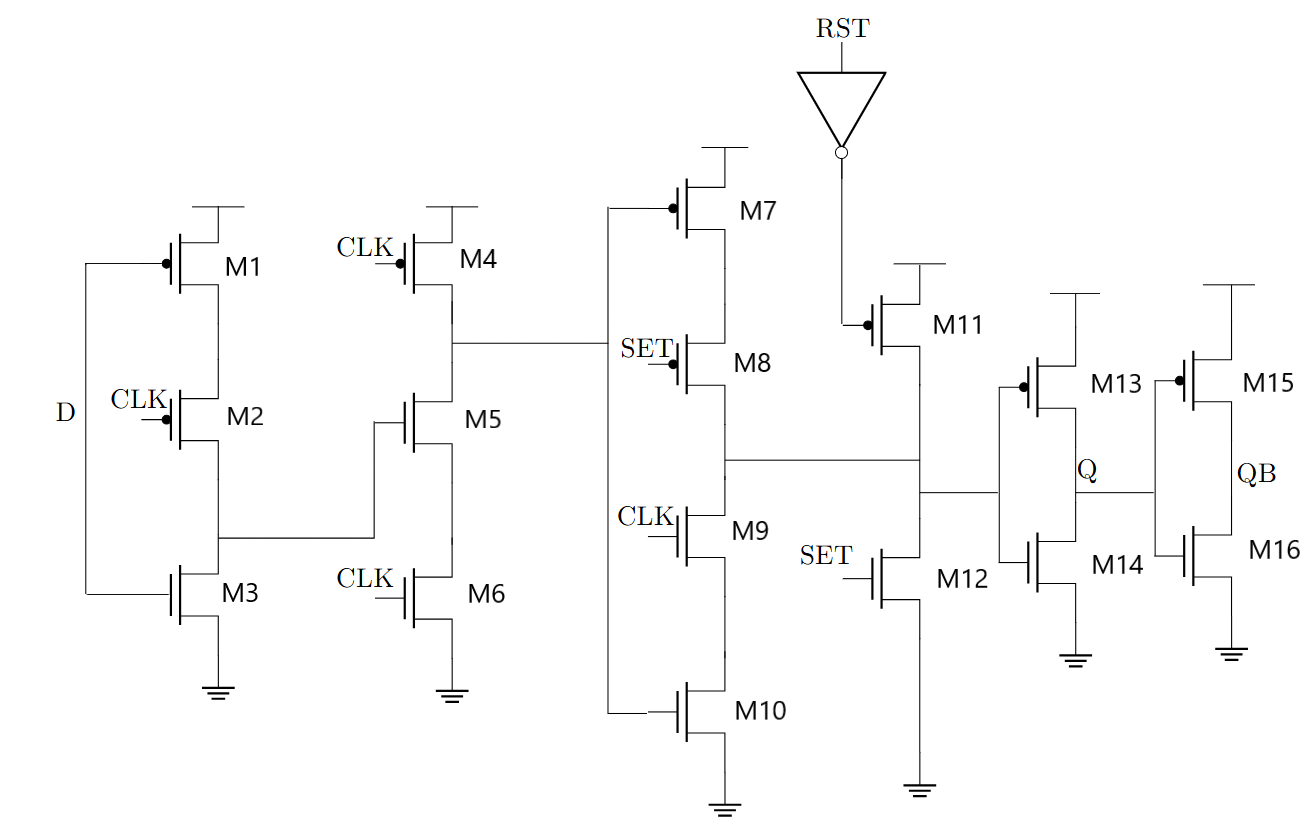
\includegraphics[width=0.8\textwidth]{chapter5/images/9.png}
	\caption{Schematic of the TSPC cell}
	\label{fig:tspc_schematic}
\end{figure}

\subsubsection{Set Operation}

When \textit{Set} is high, M12 pulls the node connected to its drain to ground, so the output
$Q$ is simply an inverter which converts 0 to $V_{DD}$.

\subsubsection{Reset Operation}

When \textit{Reset} is high, M11 turns on and pulls the node connected to its drain to
$V_{DD}$; the output is then the complement, which is 0. The inverter between the RST signal
and the gate of M11 makes the operation active-high.

\subsubsection{Buffer Operation}

When both \textit{Set} and \textit{Reset} are low and the clock is high, the output follows
the input.

\textbf{Case 1 --- Input high:} M3 turns on and pulls the node connected to its drain to
ground. The drain of M5 remains high, since M4 is off but that node was pre-charged to
$V_{DD}$ and retains its charge. Consequently, the drain of M4 is high, turning M9 and M10
on. The node connected to the drain of M9 is then pulled to ground, and $Q$---being the
inversion of that node---goes high, consistent with the high input $D$.

\textbf{Case 2 --- Input low:} The node connected to the drain of M3 is high, having been
charged to $V_{DD}$ during the low clock phase by M1 and M2. M5 and M6 then turn on and pull
the drain of M5 to ground. M7 and M8 pull the drain of M8 to $V_{DD}$, and $Q$---the
inversion of that node---goes low, consistent with the low input $D$.

\subsection{SAR Logic}
% ══════════════════════════════════════════════════════════════════════════════

The Successive Approximation Register (SAR) digital control logic is architecturally organized
into two primary functional blocks: an upper row of DFFs configured as a ring counter (or
sequencer), and a lower row acting as the data register. The operational cycle is divided into
a sampling phase and a conversion (holding) phase, sequentially executing the binary search
algorithm.

The initialization phase is governed by the global sampling signal
($\mathrm{CLK}_{\mathrm{sample}}$). During this phase, the entire register array is reset to a
known baseline state. The active-high asynchronous reset ($\mathrm{RST}$) inputs of all
subsequent flip-flops in the ring counter and data register are tied to the sampling signal,
while the asynchronous set ($\mathrm{SET}$) input of only the first DFF in the ring counter is
driven by this signal. Consequently, at the conclusion of the sampling phase, a ``one-hot''
token (a logic high) is loaded exclusively into the first stage of the ring counter, while all
remaining nodes are cleared to zero.

As the circuit transitions into the holding and conversion phase, the sampling signal goes low,
enabling the high-frequency SAR clock ($\mathrm{CLK}_{\mathrm{SAR}}$). On the first rising
edge of $\mathrm{CLK}_{\mathrm{SAR}}$, the one-hot token shifts, forcing the Most Significant
Bit ($\mathrm{B}_9$ in a 10-bit architecture) to a logic high while all lower-order bits
($\mathrm{B}_8$ through $\mathrm{B}_0$) remain low. This establishes the initial mid-scale DAC
trial code ($1000000000_2$), allowing the differential comparator to evaluate the input sample
against the DAC voltage.

Subsequent clock edges propagate the tracking token down the ring counter. The shifting token
serves as the localized clock or enable signal for the corresponding data register cells. On
the next cycle, the token activates the second MSB ($\mathrm{B}_8$). Concurrently, the digital
output of the comparator---routed globally to the data inputs ($D$) of all cells in the data
register---is clocked into the $\mathrm{B}_9$ register, permanently latching the MSB decision
as either a logic high or low based on the comparator's evaluation of the previous trial.

This iterative cycle of asserting the current trial bit and latching the previous bit decision
continues sequentially down to the Least Significant Bit ($\mathrm{B}_0$). Upon completion of
the final bit evaluation, the control logic asserts an End of Conversion ($\mathrm{EOC}$)
signal, indicating that the digital approximation of the analog input is complete and the valid
10-bit code is ready for parallel readout.

\subsubsection{SAR Logic State Table}

Table~\ref{tab:sar_state} summarizes the state of the ring counter token and the data register
bits across all 10 clock cycles of a single conversion for a 10-bit SAR ADC. The comparator
output $C$ represents the bit decision latched at each step.

\begin{table}[h!]
	\centering
	\caption{10-bit SAR logic state table (one conversion cycle)}
	\label{tab:sar_state}
	\renewcommand{\arraystretch}{1.3}
	
	\begin{tabular}{ccccccccccccc}
		\toprule
		\textbf{Cycle} &
		\textbf{Token} &
		\textbf{B\textsubscript{9}} &
		\textbf{B\textsubscript{8}} &
		\textbf{B\textsubscript{7}} &
		\textbf{B\textsubscript{6}} &
		\textbf{B\textsubscript{5}} &
		\textbf{B\textsubscript{4}} &
		\textbf{B\textsubscript{3}} &
		\textbf{B\textsubscript{2}} &
		\textbf{B\textsubscript{1}} &
		\textbf{B\textsubscript{0}} &
		\textbf{Action} \\
		\midrule
		Init & S\textsubscript{0} & 0 & 0 & 0 & 0 & 0 & 0 & 0 & 0 & 0 & 0 & Reset all; set token \\
		1    & S\textsubscript{1} & 1 & 0 & 0 & 0 & 0 & 0 & 0 & 0 & 0 & 0 & Trial B\textsubscript{9} \\
		2    & S\textsubscript{2} & C & 1 & 0 & 0 & 0 & 0 & 0 & 0 & 0 & 0 & Latch B\textsubscript{9}; trial B\textsubscript{8} \\
		3    & S\textsubscript{3} & C & C & 1 & 0 & 0 & 0 & 0 & 0 & 0 & 0 & Latch B\textsubscript{8}; trial B\textsubscript{7} \\
		4    & S\textsubscript{4} & C & C & C & 1 & 0 & 0 & 0 & 0 & 0 & 0 & Latch B\textsubscript{7}; trial B\textsubscript{6} \\
		5    & S\textsubscript{5} & C & C & C & C & 1 & 0 & 0 & 0 & 0 & 0 & Latch B\textsubscript{6}; trial B\textsubscript{5} \\
		6    & S\textsubscript{6} & C & C & C & C & C & 1 & 0 & 0 & 0 & 0 & Latch B\textsubscript{5}; trial B\textsubscript{4} \\
		7    & S\textsubscript{7} & C & C & C & C & C & C & 1 & 0 & 0 & 0 & Latch B\textsubscript{4}; trial B\textsubscript{3} \\
		8    & S\textsubscript{8} & C & C & C & C & C & C & C & 1 & 0 & 0 & Latch B\textsubscript{3}; trial B\textsubscript{2} \\
		9    & S\textsubscript{9} & C & C & C & C & C & C & C & C & 1 & 0 & Latch B\textsubscript{2}; trial B\textsubscript{1} \\
		10   & S\textsubscript{10}& C & C & C & C & C & C & C & C & C & 1 & Latch B\textsubscript{1}; trial B\textsubscript{0} \\
		EOC  & ---               & C & C & C & C & C & C & C & C & C & C & Latch B\textsubscript{0}; assert EOC \\
		\bottomrule
	\end{tabular}
\end{table}

\noindent\small$C$ = comparator decision latched from the previous trial (0 or 1);
$S_i$ = ring counter token position; EOC = End of Conversion.
\newpage
\section{Asynchronous Internal Clock Generator}

\label{sec:async_clk_gen}

To avoid relying on a fixed-frequency external clock to time the
comparator's decision and the SAR logic update, an asynchronous,
self-timed clock generator is used to produce an internal clock, $CLKC$,
directly from the external sampling clock, $CLKS$, and the comparator's
$Ready$ signal. This handshake-based approach allows the duration of each
bit-decision cycle to track the comparator's actual settling time rather
than a conservative worst-case clock period, improving conversion speed.
The circuit is shown in Fig.~\ref{fig:async_clk_gen}.

\begin{figure}[h]
	\centering
		\resizebox{\textwidth}{!}{%
	\begin{tikzpicture}[transform shape]
		% Paths, nodes and wires:
		\draw (4.375, 6.25) -| (4.375, 3.25);
		\draw (4.375, 2.75) to[short] (6.875, 4);
		\draw (6.875, 5) to[short] (4.375, 6.25);
		\draw (4.375, 3.25) to[short] (4.375, 2.75);
		\draw (6.875, 5) to[short] (6.875, 4);
		\node[shape=rectangle, minimum width=1.465cm, minimum height=0.965cm] at (5.625, 4.5){} node[anchor=north west, align=left, text width=1.077cm, inner sep=6pt] at (4.875, 5){2 to 1 MUX};
		\draw (8.875, 6.25) -| (8.875, 3.25);
		\draw (8.875, 2.75) to[short] (11.375, 4);
		\draw (11.375, 5) to[short] (8.875, 6.25);
		\draw (8.875, 3.25) to[short] (8.875, 2.75);
		\draw (11.375, 5) to[short] (11.375, 4);
		\node[shape=rectangle, minimum width=1.465cm, minimum height=0.965cm] at (10.125, 4.5){} node[anchor=north west, align=left, text width=1.077cm, inner sep=6pt] at (9.375, 5){2 to 1 MUX};
		\draw (8.875, 5) to[short] (8.125, 5);
		\draw (8.125, 5) to[short] (8.125, 4.5);
		\draw (6.875, 4.5) to[short] (8.125, 4.5);
		\draw (8.875, 4) -- (7.875, 4);
		\draw (4.375, 4) -- (3.375, 4);
		\node[ground] at (3.375, 4){};
		\node[ground] at (7.875, 4){};
		\draw (11.375, 4.5) -- (13.375, 4.5);
		\draw (5.375, 3.25) -- (5.375, 2.25);
		\draw (10.375, 3.5) -| (10.375, 2.5);
		\node[shape=rectangle, minimum width=1.965cm, minimum height=0.715cm] at (12.875, 4.875){} node[anchor=north west, align=left, text width=1.577cm, inner sep=6pt] at (11.875, 5.25){CLKC};
		\node[shape=rectangle, rotate=90, minimum width=1.965cm, minimum height=0.715cm] at (10.125, 2.5){} node[anchor=north west, align=left, text width=1.577cm, inner sep=6pt, rotate=90] at (9.75, 1.5){EOC};
		\node[shape=rectangle, rotate=90, minimum width=1.965cm, minimum height=0.715cm] at (5, 2.25){} node[anchor=north west, align=left, text width=1.577cm, inner sep=6pt, rotate=90] at (4.625, 1.25){CLKS};
		\node[latch, add async SR] at (1.13, 4.59){};
		\draw (0.01, 5.43) -| (-1, 5.5);
		\node[ieeestd not port] at (-2.907, 3.75){};
		\draw (-2.031, 3.75) -- (0.01, 3.75);
		\draw (-3.784, 3.75) -- (-4.5, 3.75);
		\node[shape=rectangle, minimum width=0.93cm, minimum height=0.465cm] at (-4.267, 4){} node[anchor=north west, align=left, text width=0.542cm, inner sep=6pt] at (-4.75, 4.25){CLKS};
		\node[shape=rectangle, minimum width=1.225cm, minimum height=0.535cm] at (-0.62, 5.715){} node[anchor=north west, align=left, text width=0.837cm, inner sep=6pt] at (-1.25, 6){VDD};
		\draw (1.13, 3.05) |- (-7, 2) -| (-7, 5) -- (-8.75, 5);
		\node[shape=rectangle, minimum width=0.93cm, minimum height=0.465cm] at (-8.5, 5.5){} node[anchor=north west, align=left, text width=0.542cm, inner sep=6pt] at (-8.983, 5.75){Ready};
		\node[ieeestd and port] at (-0.061, 9.28){};
		\node[ieeestd not port] at (-4.123, 7.5){};
		\draw (-8, 5) -| (-7, 7.5) -- (-6, 7.5);
		\draw (-3.25, 7.5) -| (-1.142, 9);
		\draw (-6, 7.5) -- (-5, 7.5);
		\draw (-6, 10.5) to[short] (-4, 10.5);
		\draw (-4, 9.5) to[short] (-4, 10.5);
		\draw (-4, 9.5) to[short] (-6, 9.5);
		\draw (-6, 9.5) to[short] (-6, 10.5);
		\node[shape=rectangle, minimum width=0.965cm, minimum height=0.465cm] at (-5.25, 10){} node[anchor=north west, align=left, text width=0.577cm, inner sep=6pt] at (-5.75, 10.25){Delay};
		\draw (-7, 7.5) |- (-6, 10);
		\draw (-4, 10) -| (-1.142, 9.56);
		\draw (1.02, 9.28) |- (1.13, 6.13);
		\draw (2.25, 5.43) -| (3.5, 5) -| (4.387, 4.749);
	\end{tikzpicture}
	
}
	\caption{Asynchronous internal clock generator block.}
	 \textbf{Note:
		the $SET$ and $RST$ inputs of the flip-flop are active-high in this
		design; the overbar (active-low) markings shown on the flip-flop
		symbol in the schematic are a drafting error and do not reflect the
		actual device behavior.}
	\label{fig:async_clk_gen}
\end{figure}

The block consists of a delay element, a two-input AND gate, an inverter,
a set/reset D flip-flop (DFF), and two cascaded 2-to-1 multiplexers. Table
\ref{tab:async_clk_signals} summarizes the function of each signal in the
circuit.

\begin{table}[h]
	\centering
	\caption{Signal description for the asynchronous clock generator.}
	\label{tab:async_clk_signals}
	\begin{tabular}{@{}p{2.2cm}p{10.5cm}@{}}
		\toprule
		Signal & Description \\
		\midrule
		$CLKS$ & External sampling clock; high during the sampling phase. \\
		$Ready$ & Asserted by the comparator once it has produced a valid
		decision, signaling that the current bit cycle is complete. \\
		$CLKC$ & Generated internal clock that times the comparator
		comparison phase and the SAR logic update. \\
		$EOC$ & End-of-conversion signal; asserted once all bits of the
		SAR cycle have been resolved. \\
		\bottomrule
	\end{tabular}
\end{table}

\paragraph{Set/reset flip-flop.}
The DFF's data input is tied to $V_{DD}$, so any active edge at its clock
input forces $Q$ high. The clock input is driven by $\overline{CLKS}$, so
$Q$ is set to $1$ when $CLKS$ falls (i.e., at the start of the conversion
phase, once sampling ends). The flip-flop's active-high reset input is
driven directly by $Ready$: once the comparator asserts $Ready$, $Q$ is
forced back to $0$, ending the high period of the internal clock.

\paragraph{Set pulse generator.}
The $Ready$ signal is also passed through a delay element and, in
parallel, through an inverter. The outputs of these two paths are combined
by an AND gate, which drives the active-high set input of the DFF. This
generates a narrow pulse that goes high only after $Ready$ has fallen
\emph{and} the delayed version of $Ready$ is still high, i.e., a short
pulse generated on the falling edge of $Ready$, delayed by the propagation
delay of the delay element. This pulse re-arms the flip-flop ($Q \to 1$)
once $Ready$ has been de-asserted, beginning the next bit cycle.

\paragraph{Multiplexing logic.}
The first multiplexer selects between $Q$ and ground based on $CLKS$: when
$CLKS$ is high (sampling phase), the multiplexer output is forced to $0$,
\emph{gating off} the internal clock; when $CLKS$ is low (conversion
phase), the multiplexer passes $Q$ through. The second multiplexer
similarly selects between the first multiplexer's output and ground based
on $EOC$: once $EOC$ is asserted at the end of the conversion, $CLKC$ is
forced low, halting the internal clock regardless of the state of $Q$.

\paragraph{Overall timing.}
The resulting behavior can be summarized as follows:

\begin{enumerate}
	\item During the sampling phase ($CLKS = 1$), $CLKC$ is held low by
	the first multiplexer, regardless of the flip-flop state.
	\item When $CLKS$ falls, marking the start of the conversion phase,
	the flip-flop is clocked and $Q$ is set high, so $CLKC$ rises,
	enabling the comparator's comparison phase and the SAR logic.
	\item Once the comparator resolves the bit and asserts $Ready$, the
	flip-flop is reset, $Q$ falls, and $CLKC$ returns low, ending the
	current bit-decision cycle.
	\item The delay-and-AND network detects the falling edge of $Ready$
	and generates a short set pulse, which re-asserts $Q$ (and therefore
	$CLKC$) to begin the next bit cycle automatically, without requiring a
	new external clock edge.
	\item This self-timed cycle repeats for each bit of the SAR
	conversion until $EOC$ is asserted, at which point the second
	multiplexer forces $CLKC$ low and the internal clock generation halts
	until the next sampling phase begins.
\end{enumerate}


\newpage

\section{Reference Voltage Bounce}
\label{sec:vref_bounce}

The voltage reference, $V_{ref}$, generated by the bandgap-driven buffer
is held on a finite decoupling capacitor, $C_{ref}$, as shown in
Fig.~\ref{fig:vref_bounce_model}. Each time the SAR logic switches a bit
of the capacitive DAC array, charge is injected onto (or removed from)
the $C_{ref}$ node through the top-plate coupling capacitance of the
switched DAC capacitor, modeled here as $\alpha C_{dac}$ and
$(1-\alpha) C_{dac}$. This charge injection causes a transient droop, or
\emph{bounce}, in $V_{ref}$, which must settle to within the converter's
resolution before the comparator's decision is latched, or the bounce
will directly corrupt the conversion result.

\begin{figure}[h]
	\centering
\resizebox{\textwidth}{!}{%
\begin{tikzpicture}[transform shape]
	% Paths, nodes and wires:
	\node[op amp] at (6.19, 3.47){};
	\draw (7.38, 3.47) -| (7.75, 5.25) |- (4.5, 5.25) -| (4.5, 4) -| (5, 3.96);
	\draw (8.75, 3.5) to[capacitor, l={$C_{ref}$}] (8.75, 1.75);
	\draw (10.25, 3.47) to[capacitor, l={$\alpha C_{DAC}$}] (12.25, 3.47);
	\draw (13.25, 3.5) to[capacitor, l={$(1-\alpha) C_{DAC}$}] (13.25, 1.75);
	\draw (5, 2.96) |- (4, 2.98);
	\draw (7.75, 3.47) -| (8.75, 3.5);
	\draw (13.25, 3.47) -- (12.25, 3.47);
	\draw (9.75, 3.5) |- (8.75, 3.47);
	\node[ground] at (13.25, 1.75){};
	\node[ground] at (8.75, 1.75){};
	\draw[dash pattern={on 1.6pt off 3.2pt}] (10.25, 5) -| (10.25, -0) -- (16.25, -0) -| (16, 5) -- (10.25, 5);
	\draw (9.75, 3.47) -- (10.25, 3.47);
	\node[shape=rectangle, minimum width=6.215cm, minimum height=0.965cm] at (14.25, 5.25){} node[anchor=north west, align=left, text width=5.827cm, inner sep=6pt] at (11.125, 5.75){Code dependent network};
	\node[shape=rectangle, minimum width=1.465cm, minimum height=0.505cm] at (4.25, 3.23){} node[anchor=north west, align=left, text width=1.077cm, inner sep=6pt] at (3.5, 3.5){VREF};
\end{tikzpicture}
		
	}
	\caption{Equivalent model of the reference buffer and the
		code-dependent DAC coupling network responsible for reference voltage
		bounce.}
	\label{fig:vref_bounce_model}
\end{figure}

\subsection{Bounce Model}

Following a switching event, $V_{ref}$ relaxes back to its nominal value
with an exponential transient set by the buffer's output resistance,
$R_{out}$, and the total capacitance at the node:

\begin{equation}
	V_{ref}(t) = V_{ref} - \Delta_i \, e^{-t/\tau},
	\label{eq:6_vref_bounce}
\end{equation}

\noindent where $\Delta_i$ is the initial voltage bounce caused by the
$i$-th switching event, and

\begin{equation}
	\tau = R_{out} \left( C_{dac} + C_{ref} \right).
	\label{eq:6_tau}
\end{equation}

The bounce magnitude is set by the charge, $Q_i$, injected onto $C_{ref}$
during switching:

\begin{equation}
	\Delta_i = \frac{Q_i}{C_{ref}}.
	\label{eq:6_delta_i}
\end{equation}

The worst-case charge injection occurs for the largest DAC capacitor
switching its full reference step under the most unfavorable coupling
ratio ($\alpha = 1/2$), giving

\begin{equation}
	Q_{i,max} = \frac{C_{dac}}{2} \cdot \frac{V_{ref}}{2},
	\label{eq:6_qimax}
\end{equation}

\noindent and therefore the worst-case bounce magnitude is

\begin{equation}
	\Delta_{i,max} = \frac{C_{dac}}{4 C_{ref}} \, V_{ref}.
	\label{eq:6_deltaimax}
\end{equation}

\subsection{Settling Requirement}

For a 10-bit converter, the reference bounce must settle to less than
half an LSB before the comparator's decision is valid, i.e.,

\begin{equation}
	\frac{C_{dac}}{4 C_{ref}} \, V_{ref} \, e^{-t/\tau} 
	\frac{1}{2} \cdot \frac{V_{ref}}{2^{10}}.
	\label{eq:6_settling_ineq}
\end{equation}

Solving \eqref{eq:6_settling_ineq} for $t$, the $V_{ref}$ and
$C_{dac}/(4C_{ref})$ terms can be rearranged to give the minimum settling
time required after each switching event:

\begin{equation}
	t > \tau \left[ 9\ln(2) - \ln\!\left(\frac{C_{ref}}{C_{dac}}\right)
	\right] = \tau \left[ 6.238 - \ln\!\left(\frac{C_{ref}}{C_{dac}}\right)
	\right],
	\label{eq:6_settling_time}
\end{equation}

\noindent where $\tau = R_{out}(C_{dac} + C_{ref})$ as defined in
\eqref{eq:6_tau}. Equation~\eqref{eq:6_settling_time} shows that the
required settling time grows logarithmically with the ratio
$C_{dac}/C_{ref}$: a larger DAC capacitance relative to the reference
decoupling capacitance increases both the worst-case bounce magnitude and
the time constant $\tau$, directly increasing the time the reference
buffer must be given to recover before the next comparator decision. This
sets a lower bound on $C_{ref}$ (or, equivalently, an upper bound on the
reference buffer's output resistance $R_{out}$) for a given target
conversion speed.
\subsection{A Practical Sizing Rule}

Equation~\eqref{eq:6_deltaimax} provides a direct and useful sizing
criterion for $C_{ref}$. Setting

\begin{equation}
	C_{ref} = 2^9 \, C_{dac},
	\label{eq:6_cref_rule}
\end{equation}

\noindent and substituting into \eqref{eq:6_deltaimax} gives

\begin{equation}
	\Delta_{i,max} = \frac{C_{dac}}{4 \left(2^9 C_{dac}\right)} V_{ref}
	= \frac{V_{ref}}{2^{11}} = \frac{1}{2}\cdot\frac{V_{ref}}{2^{10}}
	= \frac{V_{LSB}}{2}.
	\label{eq:6_cref_rule_result}
\end{equation}

That is, sizing $C_{ref}$ to be at least $2^9$ times larger than $C_{dac}$
guarantees that the \emph{initial}, worst-case bounce, $\Delta_{i,max}$,
is exactly equal to half an LSB \emph{before any settling has even
	occurred} ($t = 0$). Since the bounce decays exponentially according to
\eqref{eq:6_vref_bounce}, any non-zero settling time thereafter drives
the bounce strictly below $V_{LSB}/2$:

\begin{equation}
	\Delta_{i,max}\, e^{-t/\tau} < \frac{V_{LSB}}{2}
	\quad \text{for all } t > 0,
	\label{eq:6_cref_rule_margin}
\end{equation}

\noindent so this sizing choice provides a built-in settling margin: the
reference bounce is guaranteed to be below the resolution limit at the
moment of switching, and continues to improve throughout the remainder of
the bit-decision period, rather than only meeting the half-LSB
requirement at the end of a calculated minimum settling time as in
\eqref{eq:6_settling_time}.
\section{Voltage Reference Buffer}
\label{sec:vref_buffer}

To supply the low-impedance, well-regulated $V_{ref}$ node assumed in the
bounce analysis of Section~\ref{sec:vref_bounce}, a dedicated reference
buffer is used to drive $C_{ref}$. The buffer is implemented as a
single-stage linear regulator: an error amplifier compares the bandgap
reference voltage against the buffered output and drives an PMOS pass
transistor in a negative-feedback loop, as shown in
Fig.~\ref{fig:vref_buffer_schematic}.

\begin{figure}[h]
	\centering
\begin{tikzpicture}[transform shape]
	% Paths, nodes and wires:
	\node[op amp](N1) at (5.19, 3.51){} node[anchor=center] at (N1.text){$Error Amp$};
	\node[pmos](N2) at (8.5, 3.52){} node[anchor=west] at (N2.text){$Pass \ transistor$};
	\draw (6.38, 3.52) -| (7.52, 3.53);
	\draw (4, 4.01) -- (2.75, 4.01);
	\draw (8.5, 4.29) -- (8.5, 5.25);
	\draw (8.5, 0.875) to[dcisource, l_={$I_{bias}$}] (8.5, -0.375);
	\node[vcc] at (8.5, 5.25){};
	\draw (8.5, 0.875) -| (8.5, 1.625);
	\draw (8.5, -0.375) -| (8.5, -1.125);
	\node[ground] at (8.5, -1.125){};
	\draw (10, 1.625) to[capacitor, l={$C_{ref}$}] (10, -0.875);
	\node[ground] at (10, -0.875){};
	\draw (10, 1.625) |- (8.5, 1.625);
	\node[shape=rectangle, minimum width=1.215cm, minimum height=0.715cm] at (3.375, 4.385){} node[anchor=north west, align=left, text width=0.827cm, inner sep=6pt] at (2.75, 4.76){VREF};
	\node[shape=rectangle, minimum width=1.465cm, minimum height=0.715cm] at (9.25, 2.125){} node[anchor=north west, align=left, text width=1.077cm, inner sep=6pt] at (8.5, 2.5){Vout};
	\draw (8.5, 2.75) -| (8.5, 1.625);
	\draw (4, 2.655) |- (3, 2.625) -- (3, 1.625) -- (8.5, 1.625);
	\draw (4, 2.655) |- (4, 3.03);
\end{tikzpicture}
	\caption{Voltage reference buffer, consisting of an error amplifier
		driving an PMOS pass transistor, loaded by a bias current source and
		the reference decoupling capacitor $C_{ref}$.}
	\label{fig:vref_buffer_schematic}
\end{figure}

\subsection{Operation}

The error amplifier compares $V_{REF}$, applied at its inverting input,
against the buffer's own output, $V_{out}$, fed back to its
non-inverting input. The amplifier drives the gate of the PMOS pass
transistor, whose drain is tied to the supply and whose source delivers
$V_{out}$. This forms a negative-feedback loop that forces $V_{out}$ to
track $V_{REF}$: any deviation between $V_{out}$ and $V_{REF}$ is
amplified and corrected through the pass transistor, which adjusts its
conduction to restore $V_{out} \approx V_{REF}$ at steady state.

The output node is loaded by a fixed bias current source, $I_{bias}$,
which sets the quiescent operating current of the pass transistor, and by
the reference decoupling capacitor, $C_{ref}$, which was sized in
Section~\ref{sec:vref_bounce} to limit the transient bounce caused by
DAC switching events. The low output impedance of this regulated buffer,
$R_{out}$, together with $C_{ref}$, directly sets the bounce recovery
time constant, $\tau = R_{out}(C_{dac} + C_{ref})$, used in the bounce
analysis of \eqref{eq:6_tau}.


\section{StrongArm Comparator: Design and Simulation}


This section presents the transistor-level design of the StrongArm
comparator used in this work As discussed in Section~\ref{sec:strongarm}.  The complete
schematic, including device sizing, is shown in
Fig.~\ref{fig:strongarm_schematic}.

\begin{figure}[h]
	\centering
	
\includegraphics[width=1\textwidth]{chapter5/images/comp/sch.png}
	\caption{Transistor-level schematic of the implemented StrongArm
		comparator, with device sizing annotated.}
	\label{fig:strongarm_schematic}
\end{figure}

Table~\ref{tab:strongarm_sizing} lists the width ($W$), length ($L$), and multiplier ($m$) of every transistor
in the design, as configured in the schematic.

\begin{table}[h]
	\centering
	\caption{Transistor sizing for the StrongArm comparator.}
	\label{tab:strongarm_sizing}
	\begin{tabular}{@{}lllrrr@{}}
		\toprule
		Device & Type & Role & $W$ & $L$ & $m$ \\
		\midrule
		$M_{N1}$  & NMOS (slvtn) & Input pair (INP)                & $10.24\,\mu\text{m}$ & $20\,\text{nm}$ & 1 \\
		$M_{N2}$  & NMOS (slvtn) & Input pair (INN)                & $10.24\,\mu\text{m}$ & $20\,\text{nm}$ & 1 \\
		$M_{N5}$  & NMOS (slvtn) & Tail current / clocked switch   & $16.00\,\mu\text{m}$ & $20\,\text{nm}$ & 1 \\
		$M_{N3}$  & NMOS (slvtn) & Intermediate switch (OUTP side) & $5.12\,\mu\text{m}$  & $20\,\text{nm}$ & 1 \\
		$M_{N0}$  & NMOS (slvtn) & Intermediate switch (OUTN side) & $5.12\,\mu\text{m}$  & $20\,\text{nm}$ & 1 \\
		$M_{P9}$  & PMOS (slvtp) & Cross-coupled latch (OUTP side) & $7.68\,\mu\text{m}$  & $20\,\text{nm}$ & 1 \\
		$M_{P8}$  & PMOS (slvtp) & Cross-coupled latch (OUTN side) & $7.68\,\mu\text{m}$  & $20\,\text{nm}$ & 1 \\
		$M_{P6}$  & PMOS (slvtp) & Precharge switch                & $2.56\,\mu\text{m}$  & $20\,\text{nm}$ & 1 \\
		$M_{P7}$  & PMOS (slvtp) & Precharge switch                & $2.56\,\mu\text{m}$  & $20\,\text{nm}$ & 1 \\
		$M_{P12}$ & PMOS (slvtp) & Precharge switch (OUTP)         & $2.56\,\mu\text{m}$  & $20\,\text{nm}$ & 1 \\
		$M_{P11}$ & PMOS (slvtp) & Precharge switch (OUTN)         & $2.56\,\mu\text{m}$  & $20\,\text{nm}$ & 1 \\
		\bottomrule
	\end{tabular}
\end{table}

\noindent The input pair and tail
device are sized significantly wider than the latch and precharge devices
to maximize the input transconductance $g_m$ and bias current, which
directly set the initial voltage gain of the comparator, as derived in
\eqref{eq:5_38} and \eqref{eq:5_39}.

\subsection{Resolution and Hysteresis Verification}
To verify that the comparator resolves correctly across its entire input
range the
comparator was simulated under three differential input scenarios that
exercise the boundary conditions of correct operation: 
\begin{itemize}
	\item \textbf{Full-scale vs.\ $+1$~LSB} (Fig.~\ref{fig:res_vdd_lsb}):
	$V_{INDIFF}$ toggles between $800.0\,\text{mV}$ and $+1.6\,\text{mV}$.
	\item \textbf{Full-scale vs.\ $-1$~LSB} (Fig.~\ref{fig:res_vdd_nlsb}):
	$V_{INDIFF}$ toggles between $800.0\,\text{mV}$ and $-1.6\,\text{mV}$.
	\item \textbf{$+1$~LSB vs.\ $-1$~LSB} (Fig.~\ref{fig:res_lsb_nlsb}):
	$V_{INDIFF}$ toggles between $+1.6\,\text{mV}$ and $-1.6\,\text{mV}$.
\end{itemize}
\begin{figure}[h]
	\centering
	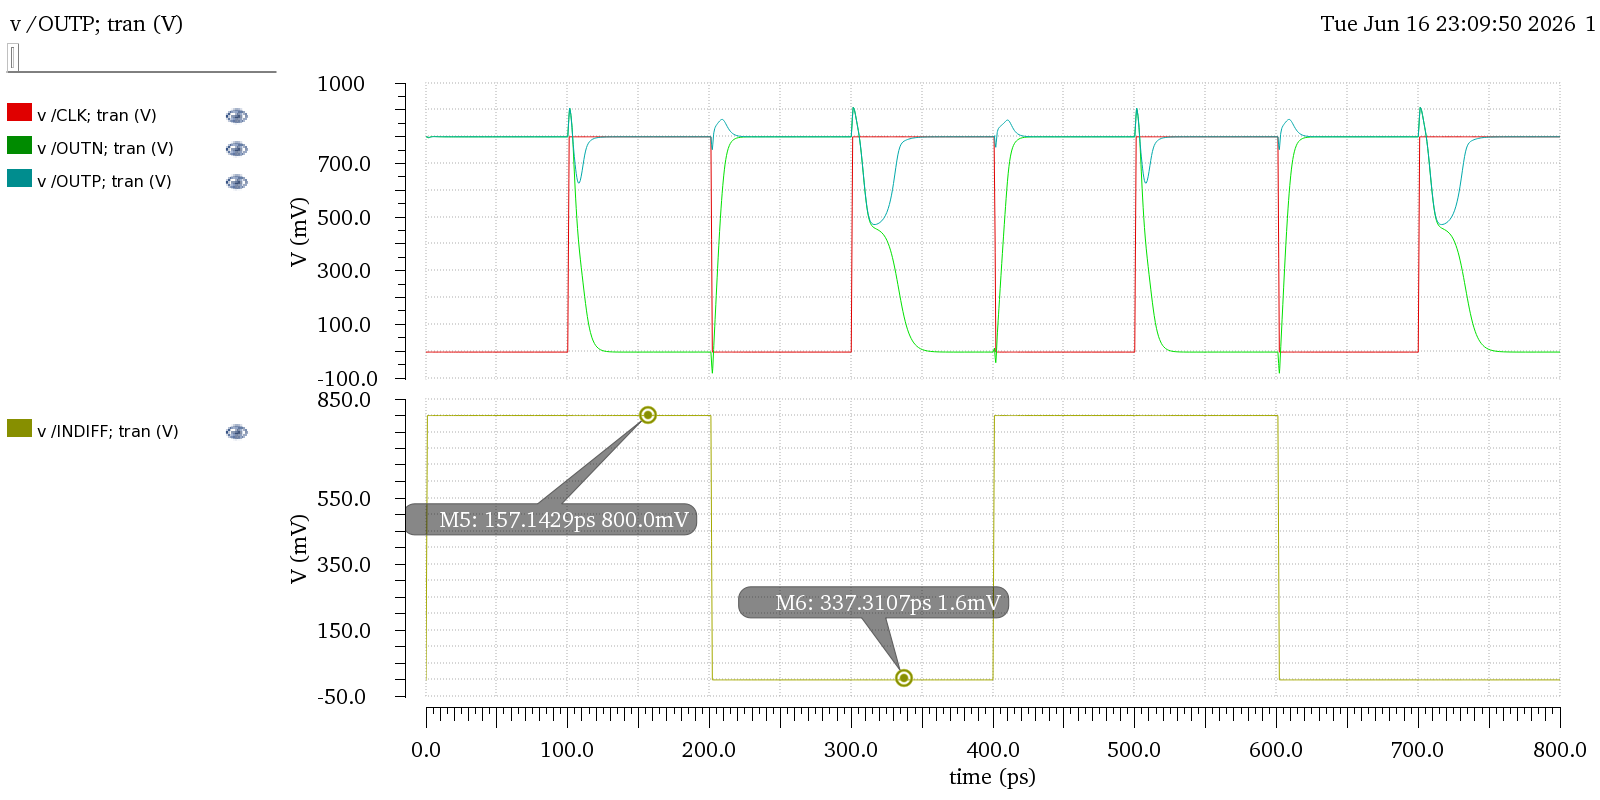
\includegraphics[width=0.95\textwidth]{chapter5/images/comp/VDD_LSB.png}
	\caption{Comparator response with $V_{INDIFF}$ toggling between
		full-scale ($800.0\,\text{mV}$) and $+1$~LSB ($1.6\,\text{mV}$).}
	\label{fig:res_vdd_lsb}
\end{figure}

\begin{figure}[h]
	\centering
	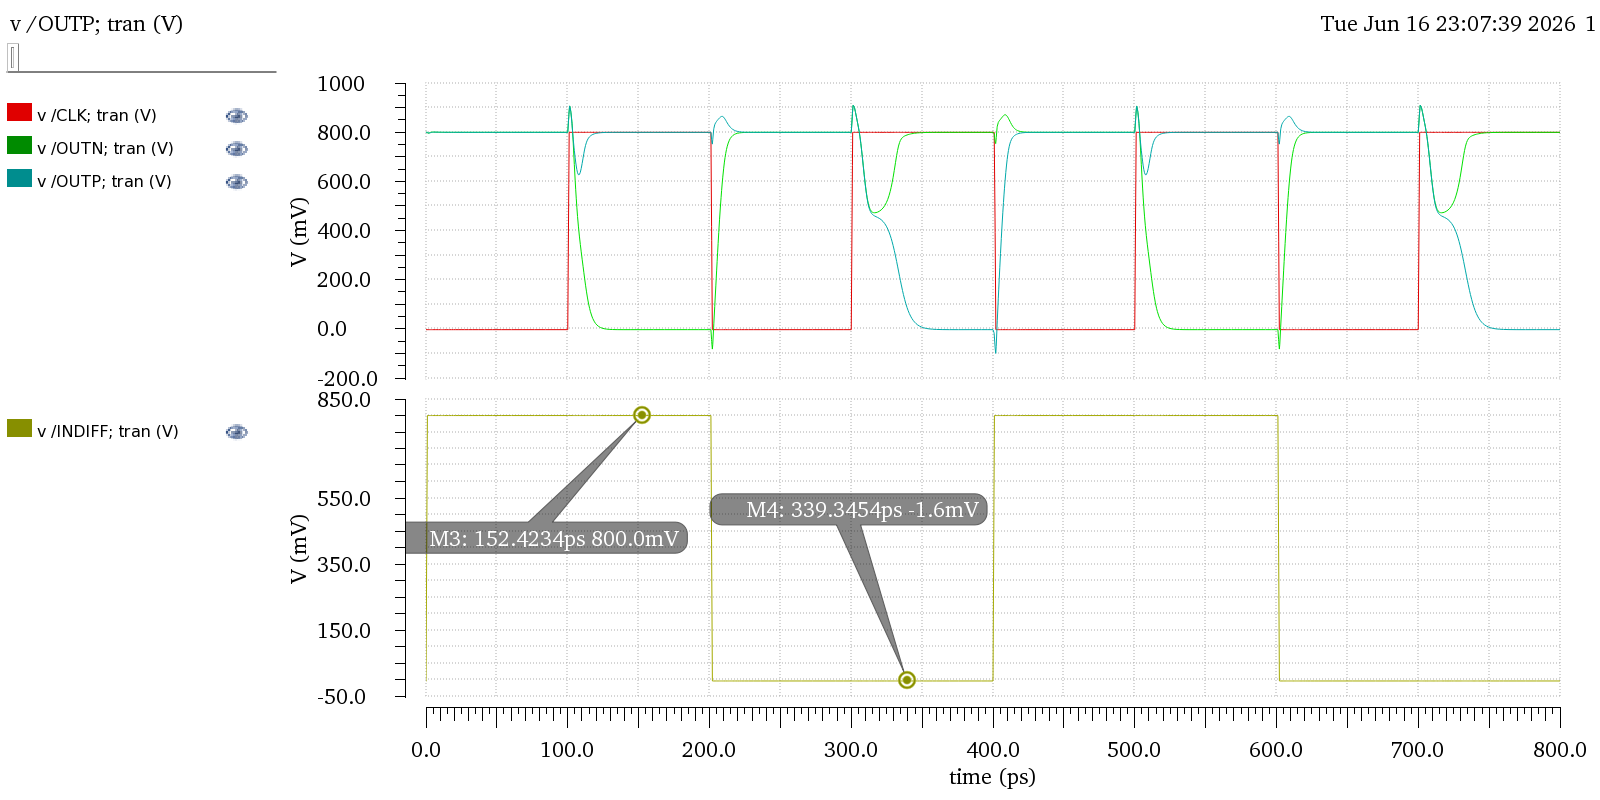
\includegraphics[width=0.95\textwidth]{chapter5/images/comp/VDD_NLSB.png}
	\caption{Comparator response with $V_{INDIFF}$ toggling between
		full-scale ($800.0\,\text{mV}$) and $-1$~LSB ($-1.6\,\text{mV}$).}
	\label{fig:res_vdd_nlsb}
\end{figure}
\newpage
\begin{figure}[h]
	\centering
	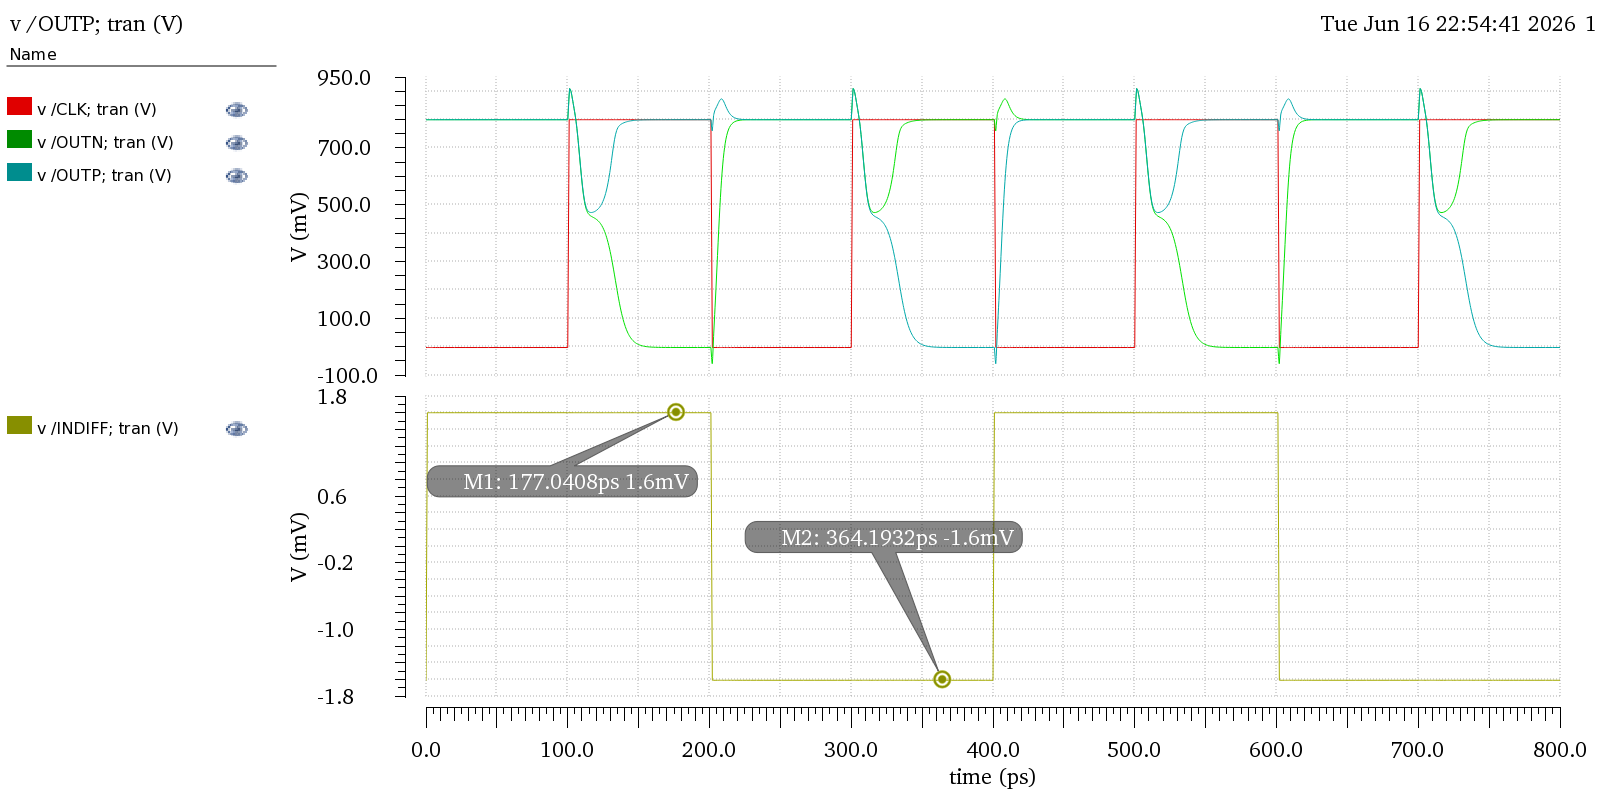
\includegraphics[width=0.95\textwidth]{chapter5/images/comp/LSB_NLSB.png}
	\caption{Comparator response with $V_{INDIFF}$ toggling between
		$+1$~LSB ($1.6\,\text{mV}$) and $-1$~LSB ($-1.6\,\text{mV}$), the
		minimum resolvable differential input.}
	\label{fig:res_lsb_nlsb}
\end{figure}
In all three cases, the comparator regenerates a full-swing, correctly
polarized output on every clock cycle: $OUTP$ and $OUTN$ resolve high and
low (or vice versa) consistently with the sign of $V_{INDIFF}$, with no
missed decisions, no metastable (partially-resolved) outputs, and no
dependence of a given decision on the outcome of the previous cycle.

\subsection{Decision Delay vs.\ Input Differential Voltage}

The comparator's regeneration delay, $t_d$, was characterized as a
function of the input differential voltage, $\Delta V_{in}$, by sweeping
$\Delta V_{in}$ logarithmically and measuring the time required for the
output to resolve.The delay is expected to scale as

\begin{equation}
	t_d = \tau \ln\!\left(\frac{V_{FS}}{\Delta V_{in}}\right)
	= \tau \ln(V_{FS}) - \tau \ln(\Delta V_{in}),
	\label{eq:5_42}
\end{equation}

\noindent where $V_{FS}$ is the full-scale input voltage and $\tau$ is the
regeneration time constant of the cross-coupled latch. which is confirmed by the simulated delay characteristic shown
in Fig.~\ref{fig:delay_vs_vin}, plotted on a logarithmic $\Delta V_{in}$
axis.

\begin{figure}[h]
	\centering
	\includegraphics[width=0.95\textwidth]{chapter5/images/comp/delay.png}
	\caption{Comparator decision delay, $t_d$, as a function of input
		differential voltage, $\Delta V_{in}$, on a logarithmic axis.}
	\label{fig:delay_vs_vin}
\end{figure}

The maximum decision delay, $t_{d,max} = 47.81\,\text{ps}$, occurs at the
smallest simulated input, $\Delta V_{in} = 1.6\,\text{mV}$ (the minimum
resolvable LSB-level input), while the minimum decision delay,
$t_{d,min} = 21.07\,\text{ps}$, occurs at the largest simulated input,
$\Delta V_{in} = 751.6\,\text{mV}$ (near full scale). Since the comparator
must resolve even its smallest specified input within one clock period,
$t_{d,max}$ sets the worst-case timing constraint and therefore limits the
maximum clock frequency at which the comparator can operate reliably to
approximately

\begin{equation}
	f_{clk,max} \approx \frac{1}{t_{d,max}} \approx 20.9\,\text{GHz}.
	\label{eq:5_43}
\end{equation}

\noindent This bound assumes the entire clock period is available for
regeneration; in a complete SAR ADC, additional margin must be reserved
for the sampling phase and SAR logic update, so the practically achievable
conversion rate will be correspondingly lower than this comparator-limited
bound.
\subsubsection{Decision Delay Across Process and Temperature Corners}
\label{sec:strongarm_delay_corners}

To verify that the comparator meets its timing requirements across the
full range of expected manufacturing and environmental variation, the
decision delay versus input differential voltage characteristic was re-simulated at the two
extreme process/voltage/temperature (PVT) corners: the slow-slow (SS)
corner at $125^\circ\text{C}$ and $-5\%$ $V_{DD}$, representing the
worst-case (slowest) operating condition, and the fast-fast (FF) corner
at $-40^\circ\text{C}$ and $+5\%$ $V_{DD}$, representing the best-case
(fastest) operating condition. The resulting delay characteristics are
shown in Fig.~\ref{fig:delay_vs_vin_corners}.

\begin{figure}[h]
	\centering
	
\includegraphics[width=0.85\textwidth]{chapter5/images/comp/co.png}
	\caption{Comparator decision delay, $t_d$, versus input differential
		voltage, $\Delta V_{in}$, at the SS ($125^\circ\text{C}$,
		$-5\%\,V_{DD}$) and FF ($-40^\circ\text{C}$, $+5\%\,V_{DD}$) process
		corners.}
	\label{fig:delay_vs_vin_corners}
\end{figure}



As expected, the SS corner exhibits the largest decision delay at every
value of $\Delta V_{in}$, since both the reduced supply voltage and
elevated temperature degrade the transistors' transconductance and
increase their threshold voltage, slowing the regenerative latch's
time constant, $\tau$, in \eqref{eq:5_42}. Conversely, the FF corner
exhibits the smallest decision delay, benefiting from both a higher
supply voltage and improved carrier mobility at low temperature.
\subsection{Power Consumption vs.\ Operating Frequency}


Since the StrongArm comparator has no static bias current and draws power
only during its clocked precharge and regeneration phases, its power
consumption is expected to scale approximately linearly with the clock
frequency, $f_{clk}$, dominated by the dynamic switching energy consumed
each cycle. To verify this, the comparator's average supply current was
simulated while sweeping $f_{clk}$ from $300\,\text{MHz}$ to $3.0\,\text{GHz}$,
with the resulting power consumption shown in
Fig.~\ref{fig:power_vs_freq}.
\begin{table}[h]
	\centering
	\caption{Comparator power consumption at minimum and maximum simulated
		clock frequency.}
	\label{tab:power_vs_freq}
	\begin{tabular}{@{}lcc@{}}
		\toprule
		& $f_{clk}$ & Power \\
		\midrule
		Minimum & $300\,\text{MHz}$ & $13.418\,\mu\text{W}$ \\
		Maximum & $3.0\,\text{GHz}$ & $122.077\,\mu\text{W}$ \\
		\bottomrule
	\end{tabular}
\end{table}

\begin{figure}[h]
	\centering
	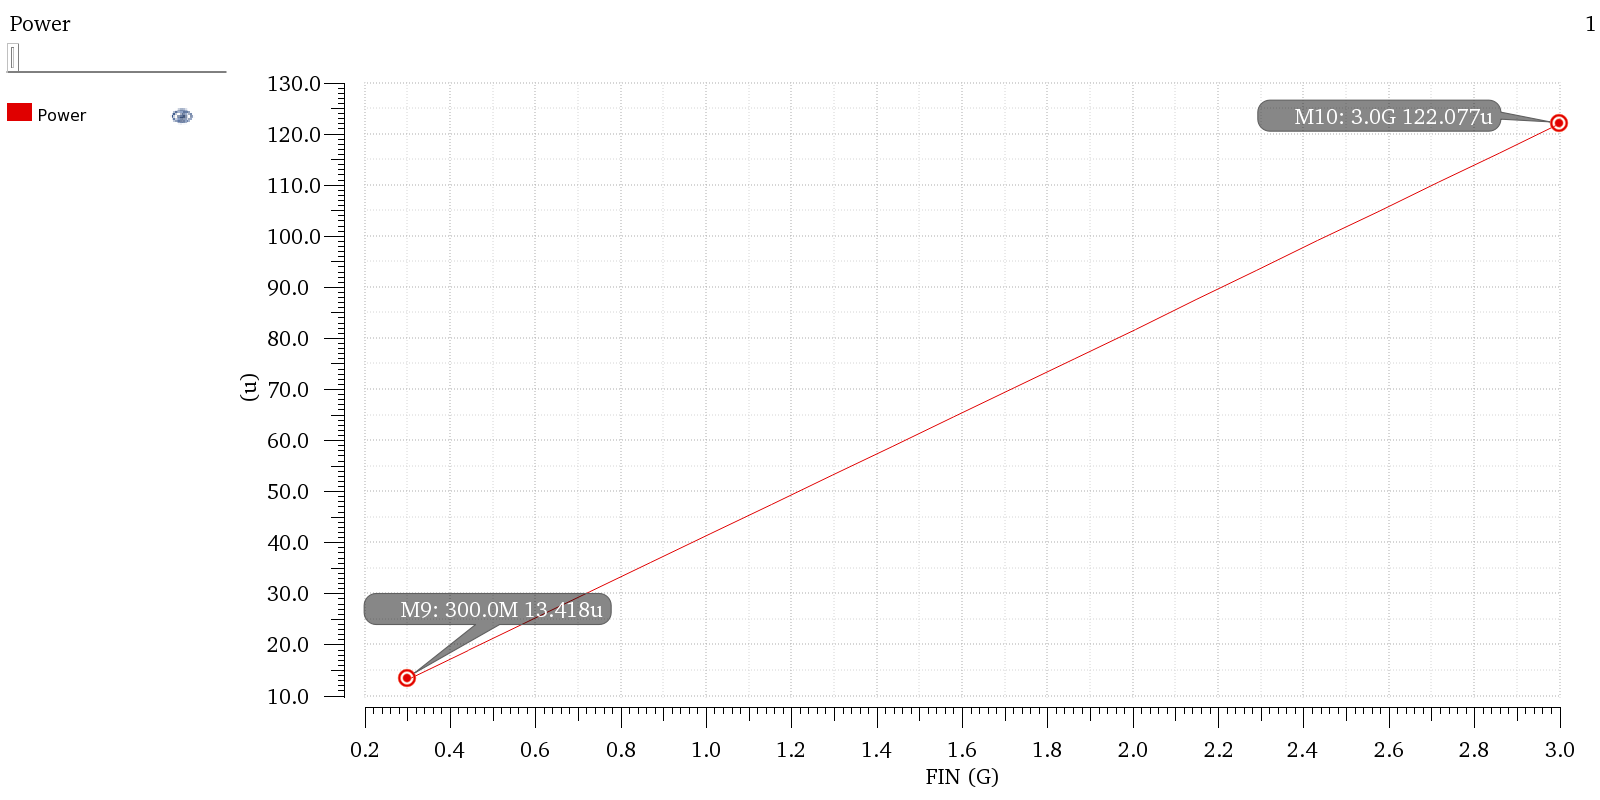
\includegraphics[width=0.95\textwidth]{chapter5/images/comp/Power.png}
	\caption{Comparator power consumption as a function of clock
		frequency, $f_{clk}$.}
	\label{fig:power_vs_freq}
\end{figure}
\subsection{Thermal Noise}
Using noise simulation procedure in Analysis and Design of Data Converters textbook the $V_{nrms}= 200 uV$ 
\subsection{Input-Referred Offset: Monte Carlo Mismatch Analysis}
\label{sec:strongarm_offset_mc}

As discussed in Section~\ref{sec:strongarm}, device mismatch among
the input pair and the cross-coupled latch transistors introduces a
random input-referred offset, $V_{OS}$, as expressed analytically in
\eqref{eq:5_39}. To statistically characterize this offset for the actual
fabricated device sizes, a Monte Carlo simulation with $N = 500$ runs was
performed, applying random process and mismatch variations to all
transistors in the comparator. The resulting offset distribution is shown
in Fig.~\ref{fig:offset_montecarlo}.

\begin{figure}[h]
	\centering
		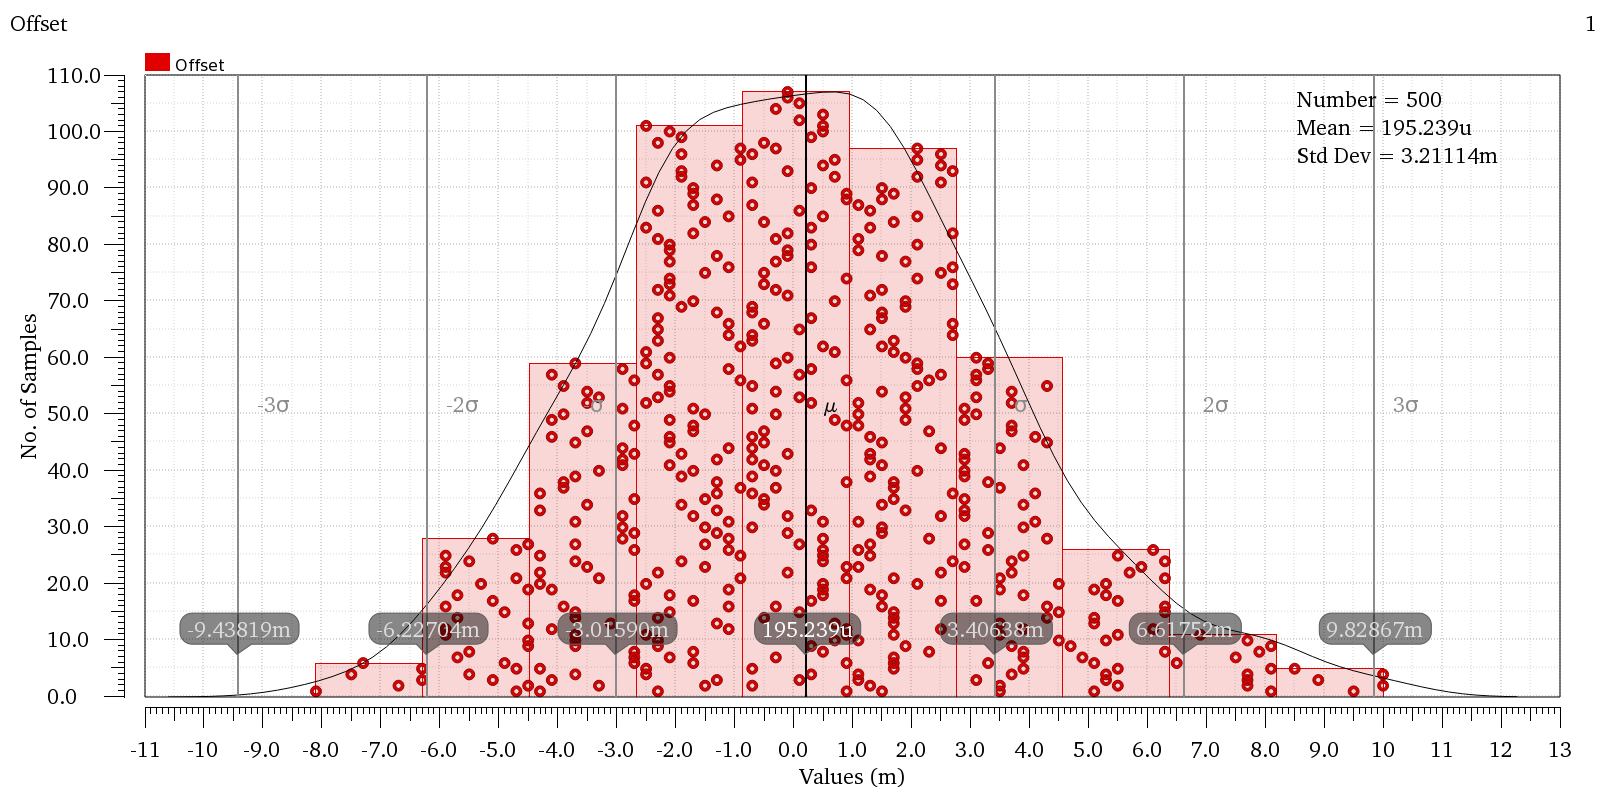
\includegraphics[width=0.95\textwidth]{chapter5/images/comp/Offset.png}
	\caption{Monte Carlo distribution of comparator input-referred offset
		due to device mismatch ($N = 500$ runs).}
	\label{fig:offset_montecarlo}
\end{figure}

The extracted distribution has a mean of $\mu = 195.24\,\mu\text{V}$ and a
standard deviation of $\sigma = 3.211\,\text{mV}$.Across the simulated population, the offset spans
approximately $\pm 3\sigma$, i.e.\ from $-9.44\,\text{mV}$ to
$+9.83\,\text{mV}$, which represents the expected worst-case offset range
for the vast majority ($99.7\,\%$) of fabricated devices.

\section{Capacitive DAC: Design and Simulation}
% ══════════════════════════════════════════════════════════════════════════════

As we explained in the literature section, the configuration of the capacitive DAC differs
according to the application, so our choice was to use a split DAC and inherit a sample-and-hold
circuit.

We need to characterize the mismatch between the caps from the PDK to estimate the DNL
produced by the cap DAC, where

\begin{equation}
	\sigma_{\mathrm{DNL_{Bridged}}} = 2^{M} \times 2^{K-1} \times \sigma_{C_u}
\end{equation}

So, we need to achieve a maximum DNL less than 0.5\,LSB, then

\begin{equation}
	3\sigma = 0.5\,\mathrm{LSB} \quad \Rightarrow \quad \text{Yield } 99.73\%
\end{equation}
\begin{equation}
	\sigma = 166\,\mathrm{mLSB}
\end{equation}

The choice of the unit cap was very important; its value, which corresponds to its area, plays a
main role in determining the DNL from the CAP DAC. We characterized the mismatch of the caps in
22\,nm technology using MOM10V caps, which can achieve lower values down to \SI{2}{fF} for
minimum area.

\begin{figure}[h!]
	\centering
	
\includegraphics[width=0.3\textwidth]{chapter5/images/1.png}
	\caption{Testbench for caps mismatch characterization}
	\label{fig:testbench}
\end{figure}

In Fig.~\ref{fig:testbench}, the testbench we used was an AC current source connected to two
parallel caps, identical in size and values. We then ran an AC analysis and obtained the values
of the two caps as follows:

\begin{equation}
	C = -\frac{1}{\operatorname{imag}(V_1) \cdot I_1 \cdot \omega}
\end{equation}

\begin{equation}
	\frac{\Delta C}{C} = \frac{C_1 - C_2}{\operatorname{avg}(C_1, C_2)}
\end{equation}

We computed the difference between the two capacitors divided by their nominal value. Using a
Monte Carlo simulation, we obtained the mismatch between them and determined the minimum cap
size needed to achieve the required DNL for the binary and bridged cap DAC.

So, the mismatch between two caps should satisfy

\begin{equation}
	\sigma_{C_{u,\min}} = \frac{166\,\mathrm{m}}{27.5} \approx 1\,\mathrm{mLSB} \quad
	\text{(bridged)}
\end{equation}

\begin{figure}[h!]
	\centering
	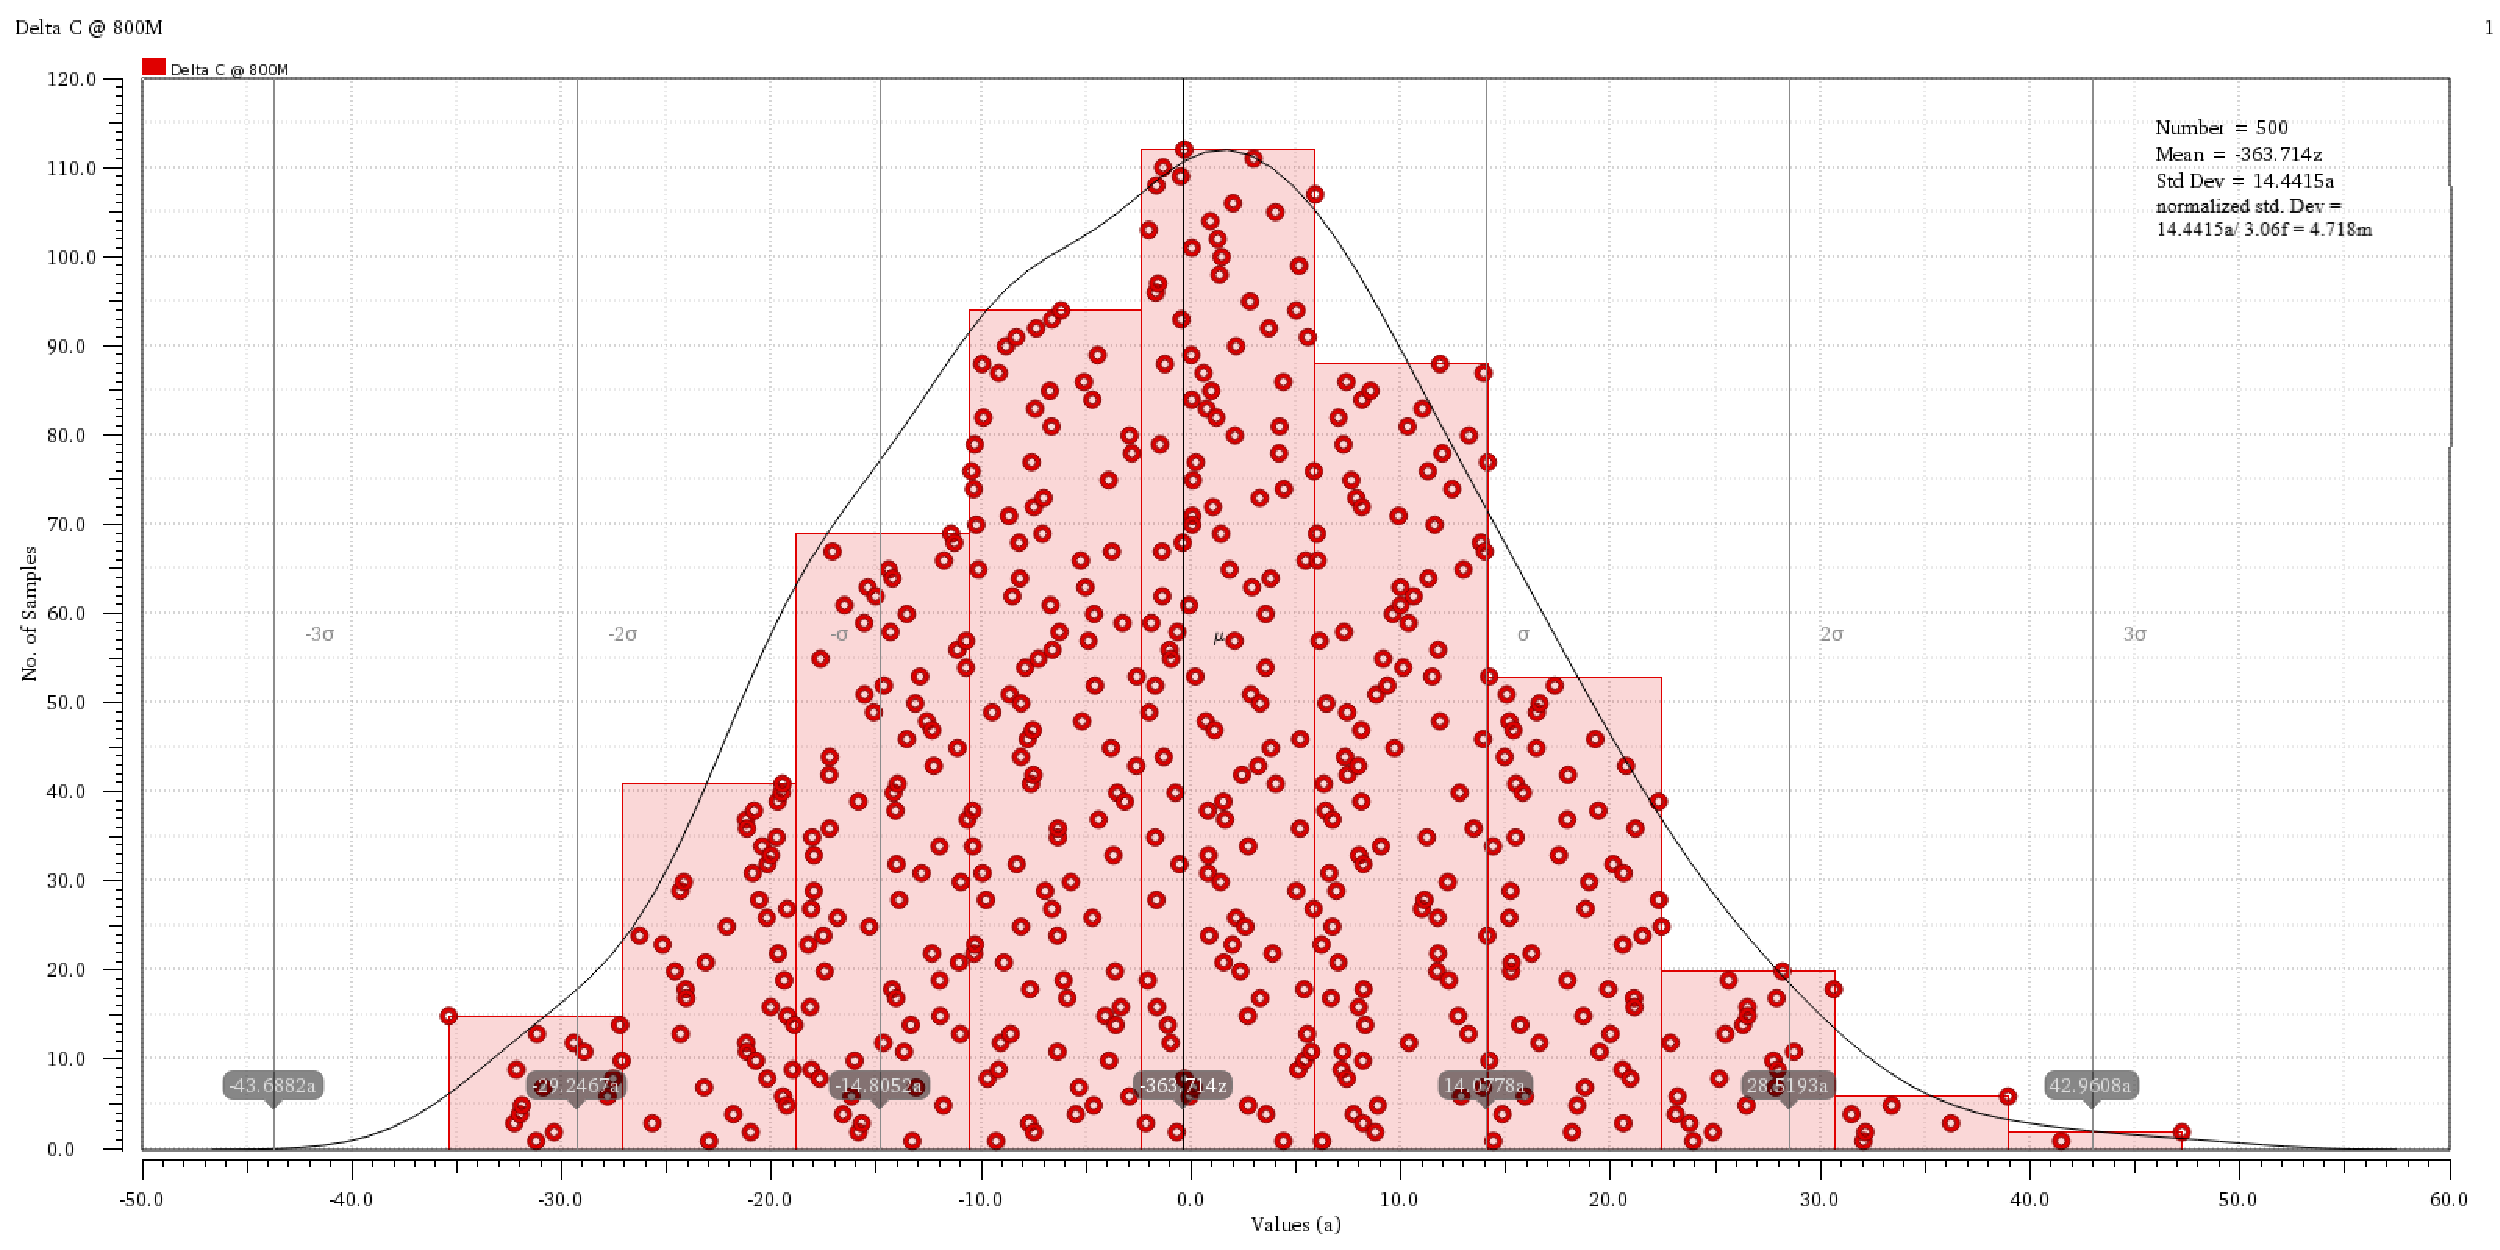
\includegraphics[width=0.8\textwidth]{chapter5/images/2.pdf}
	\caption{Caps mismatch for $3\,\mu\mathrm{m} \times 3\,\mu\mathrm{m}$ area}
	\label{fig:mismatch_3x3}
\end{figure}

\begin{figure}[h!]
	\centering
	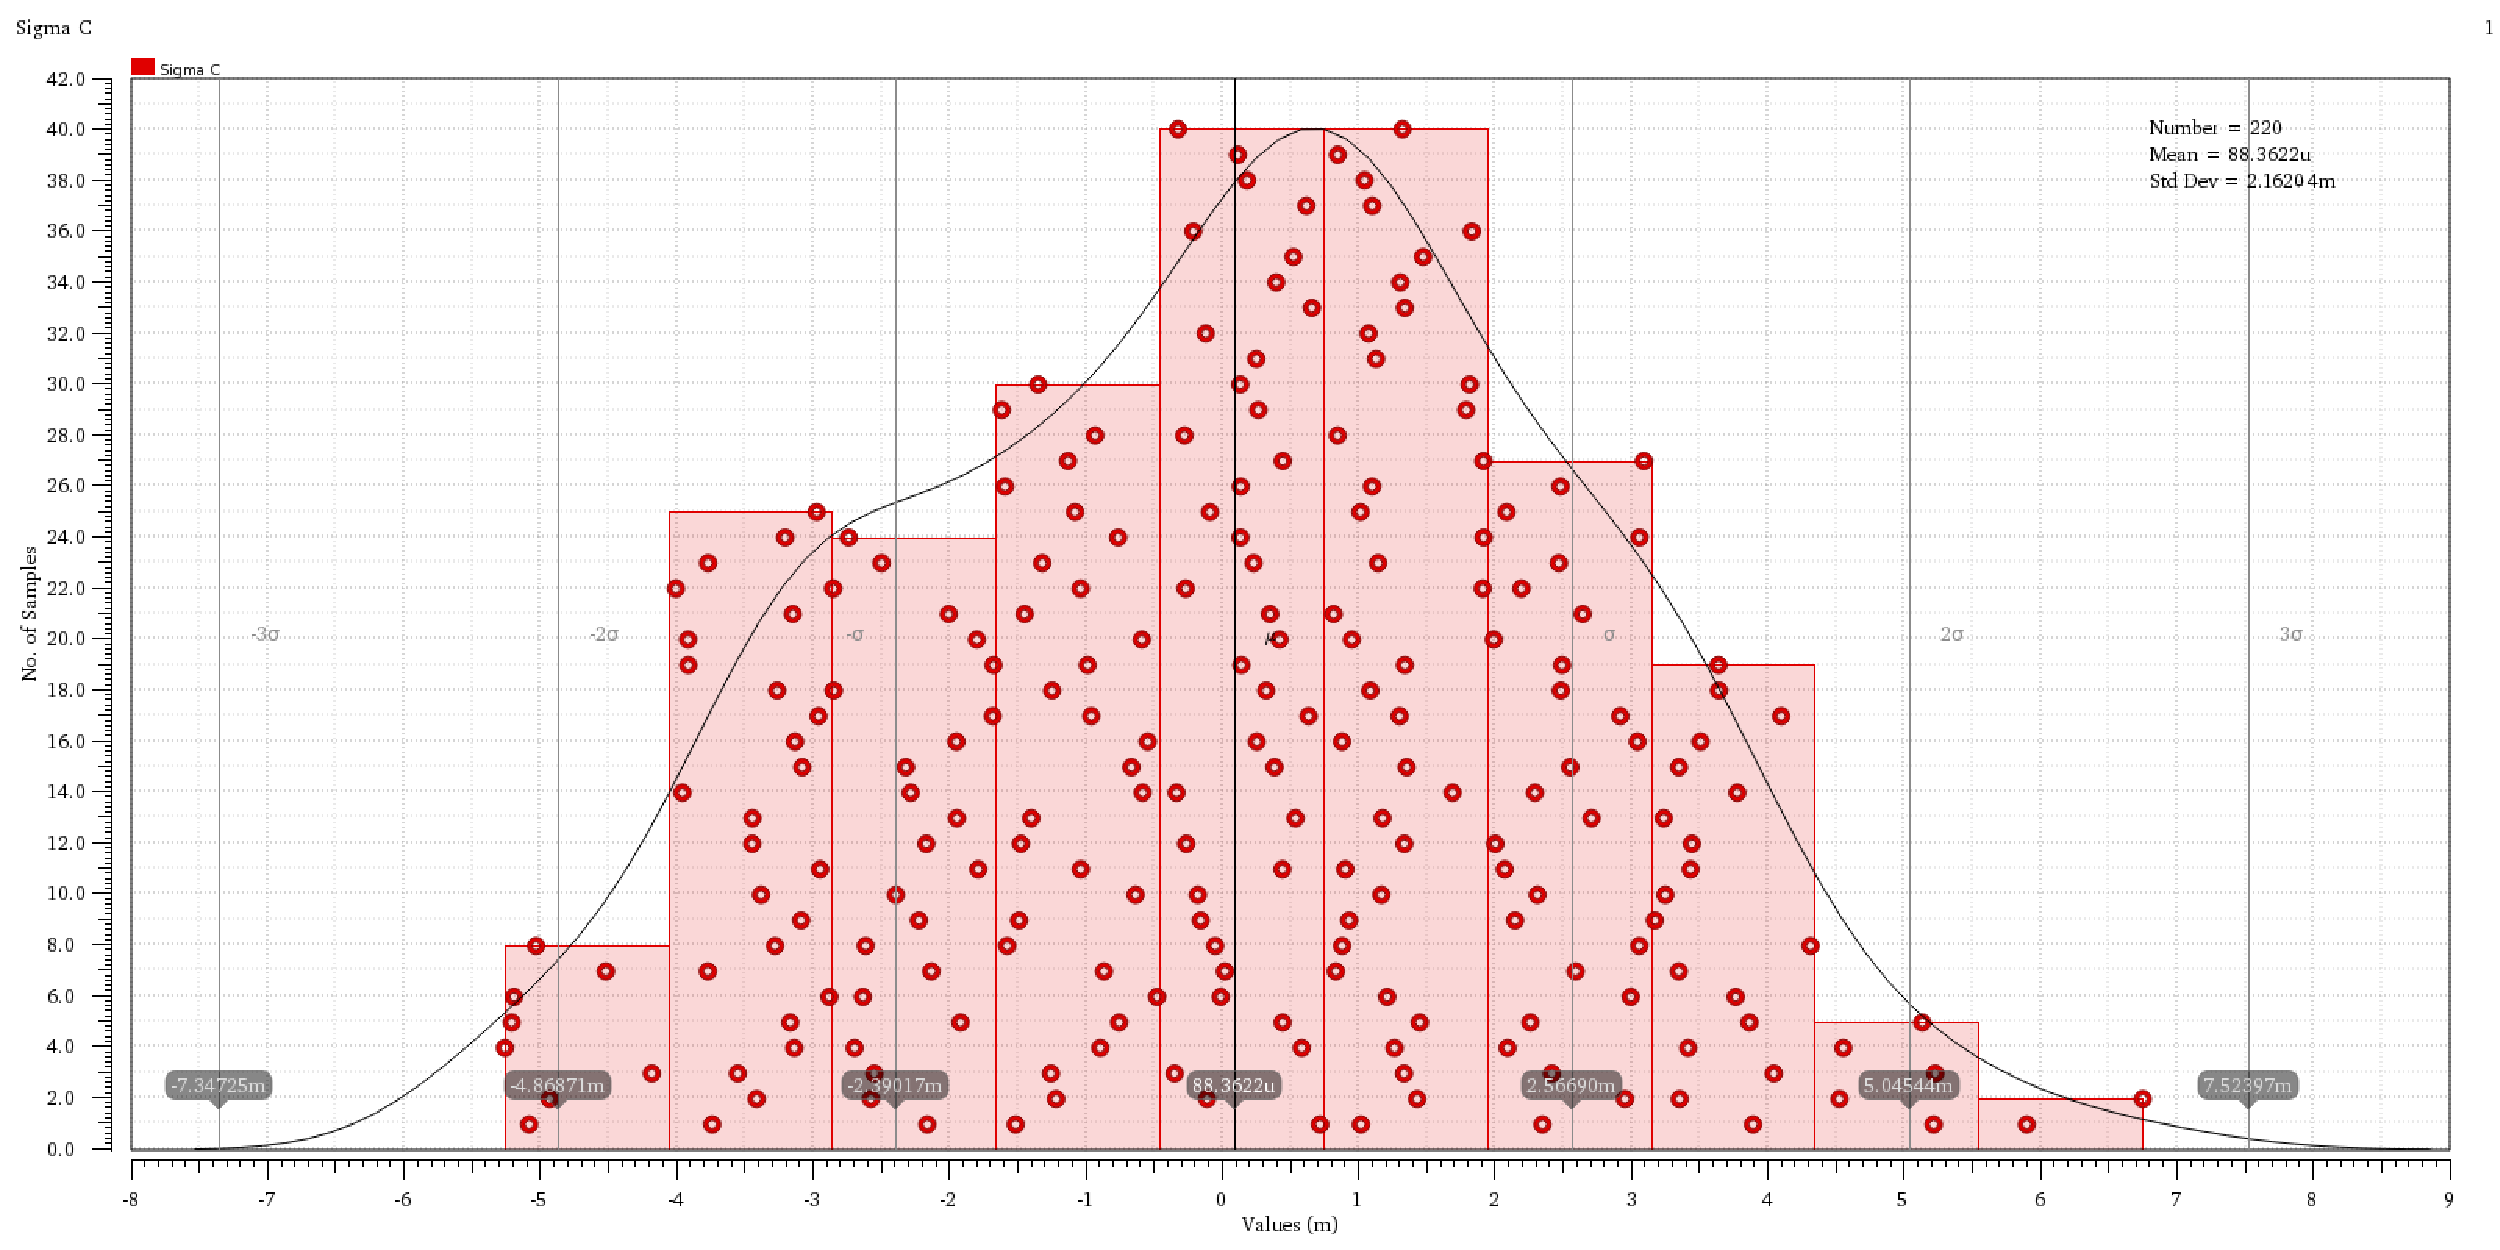
\includegraphics[width=0.8\textwidth]{chapter5/images/3.pdf}
	\caption{Caps mismatch for $15\,\mu\mathrm{m} \times 10\,\mu\mathrm{m}$ area}
	\label{fig:mismatch_15x10}
\end{figure}

From Fig.~\ref{fig:mismatch_15x10}, the value used for the unit capacitor is approximately
\SI{35}{fF}. This value achieves a standard deviation of \SI{2.1}{mLSB}. We then simulated
the DNL for the whole bridged capacitor, and that value achieved the required standard deviation
of the DNL as shown in Fig.~\ref{fig:dnl_stats}.

\begin{figure}[h!]
	\centering
	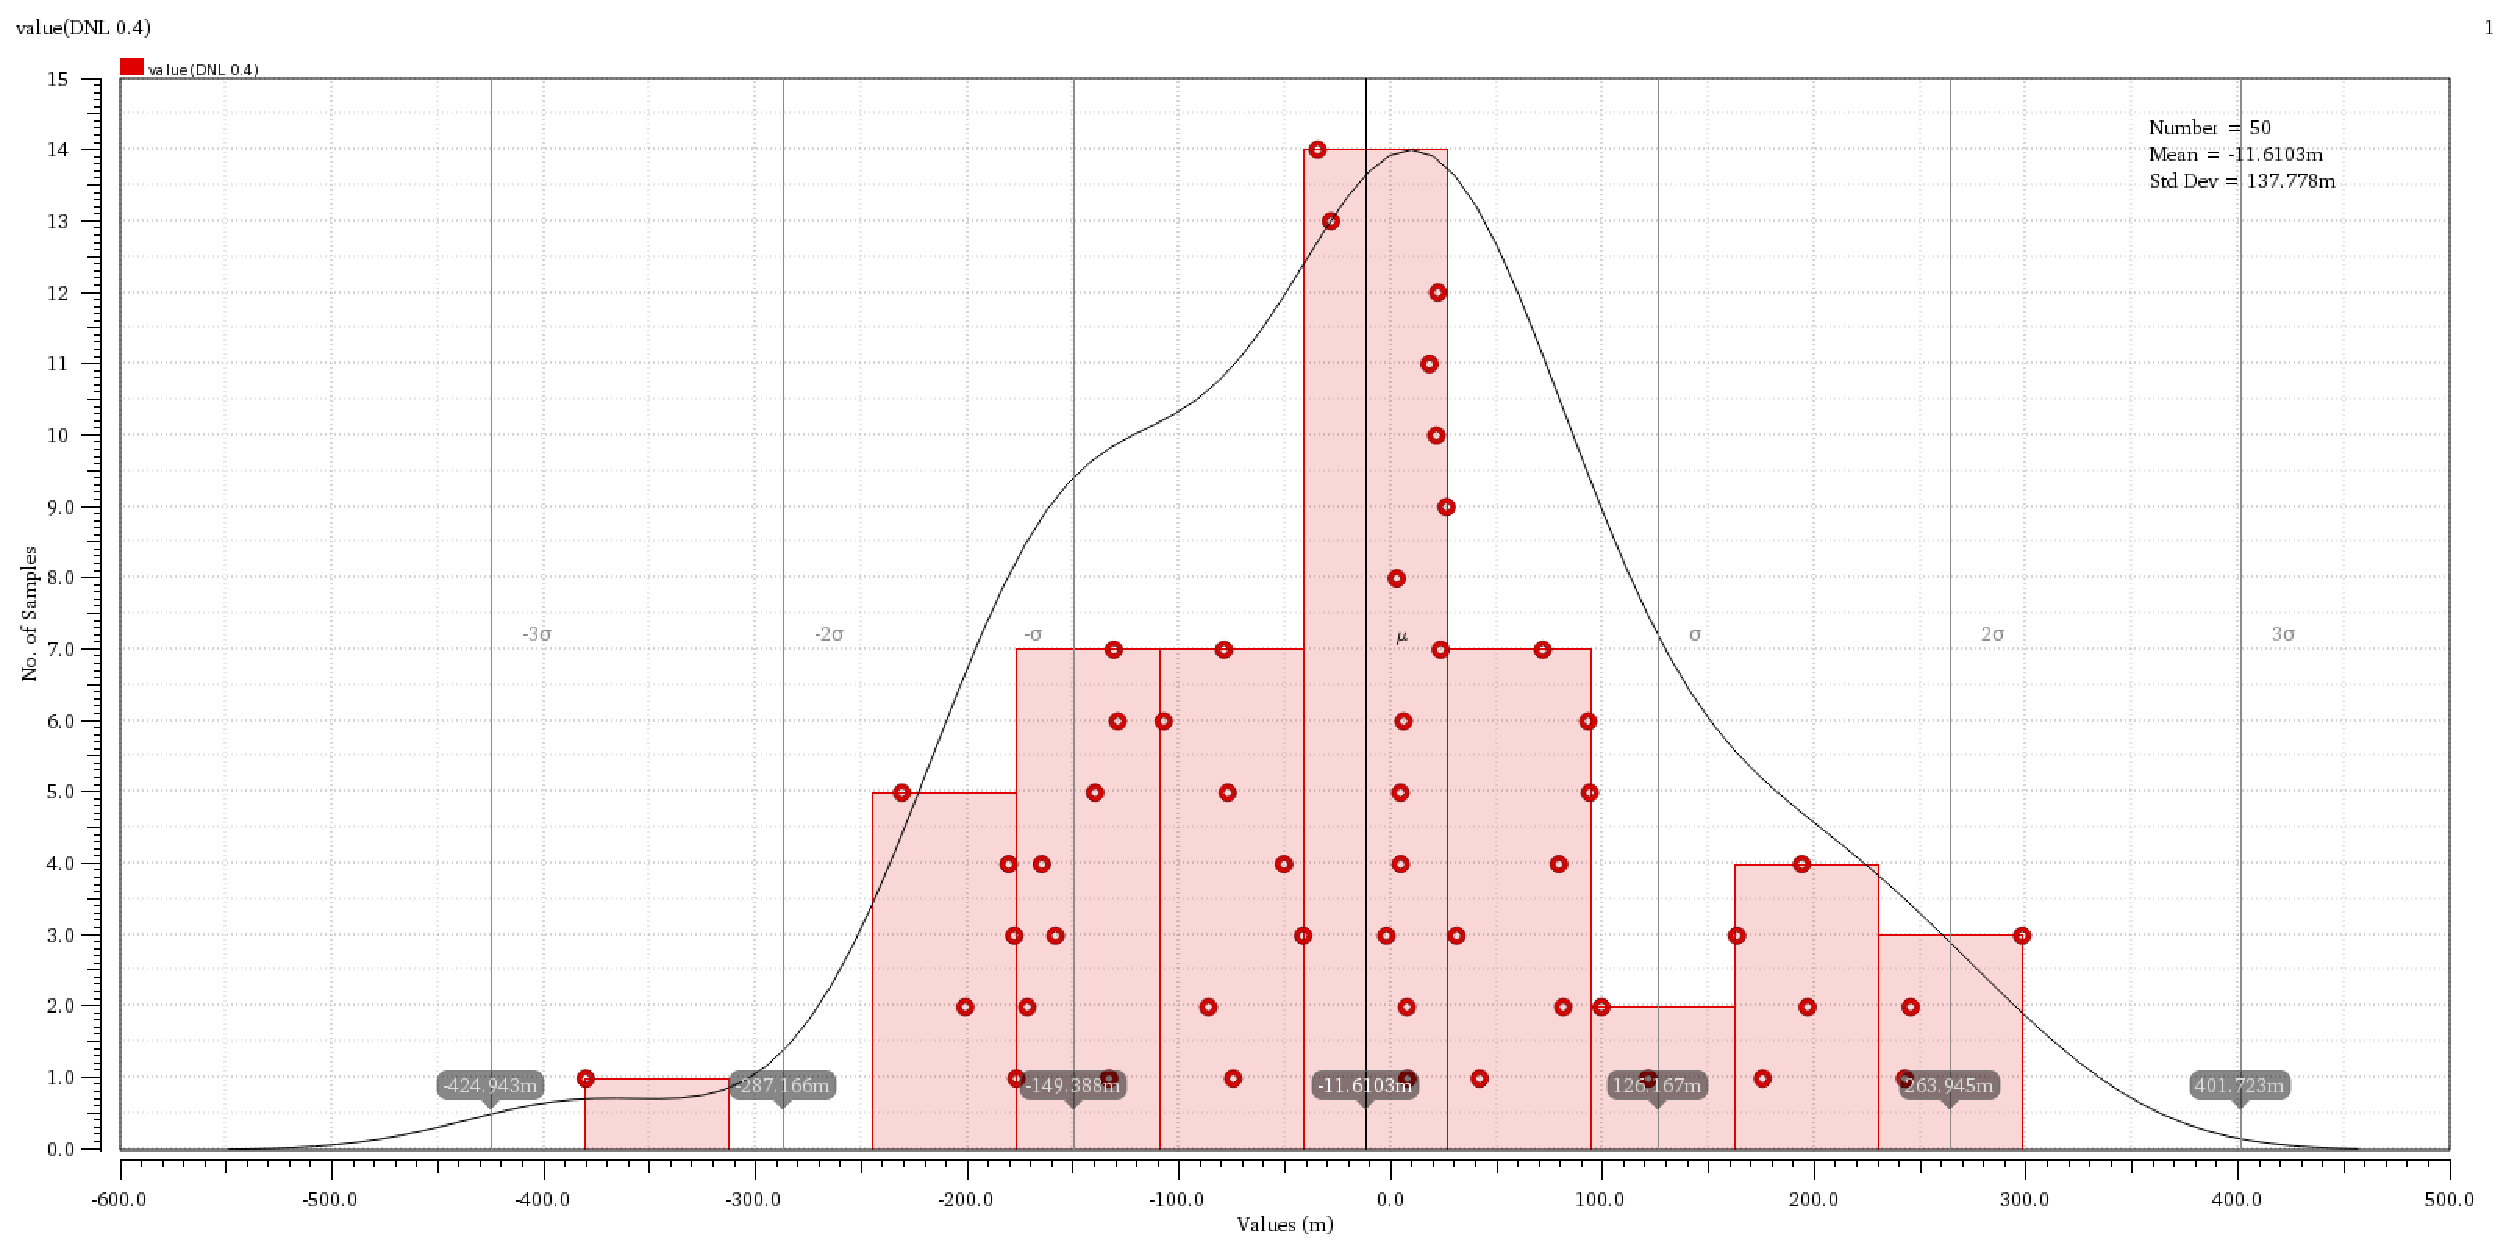
\includegraphics[width=0.8\textwidth]{chapter5/images/4.pdf}
	\caption{DNL statistics for bridged cap}
	\label{fig:dnl_stats}
\end{figure}

\begin{figure}[h!]
	\centering
	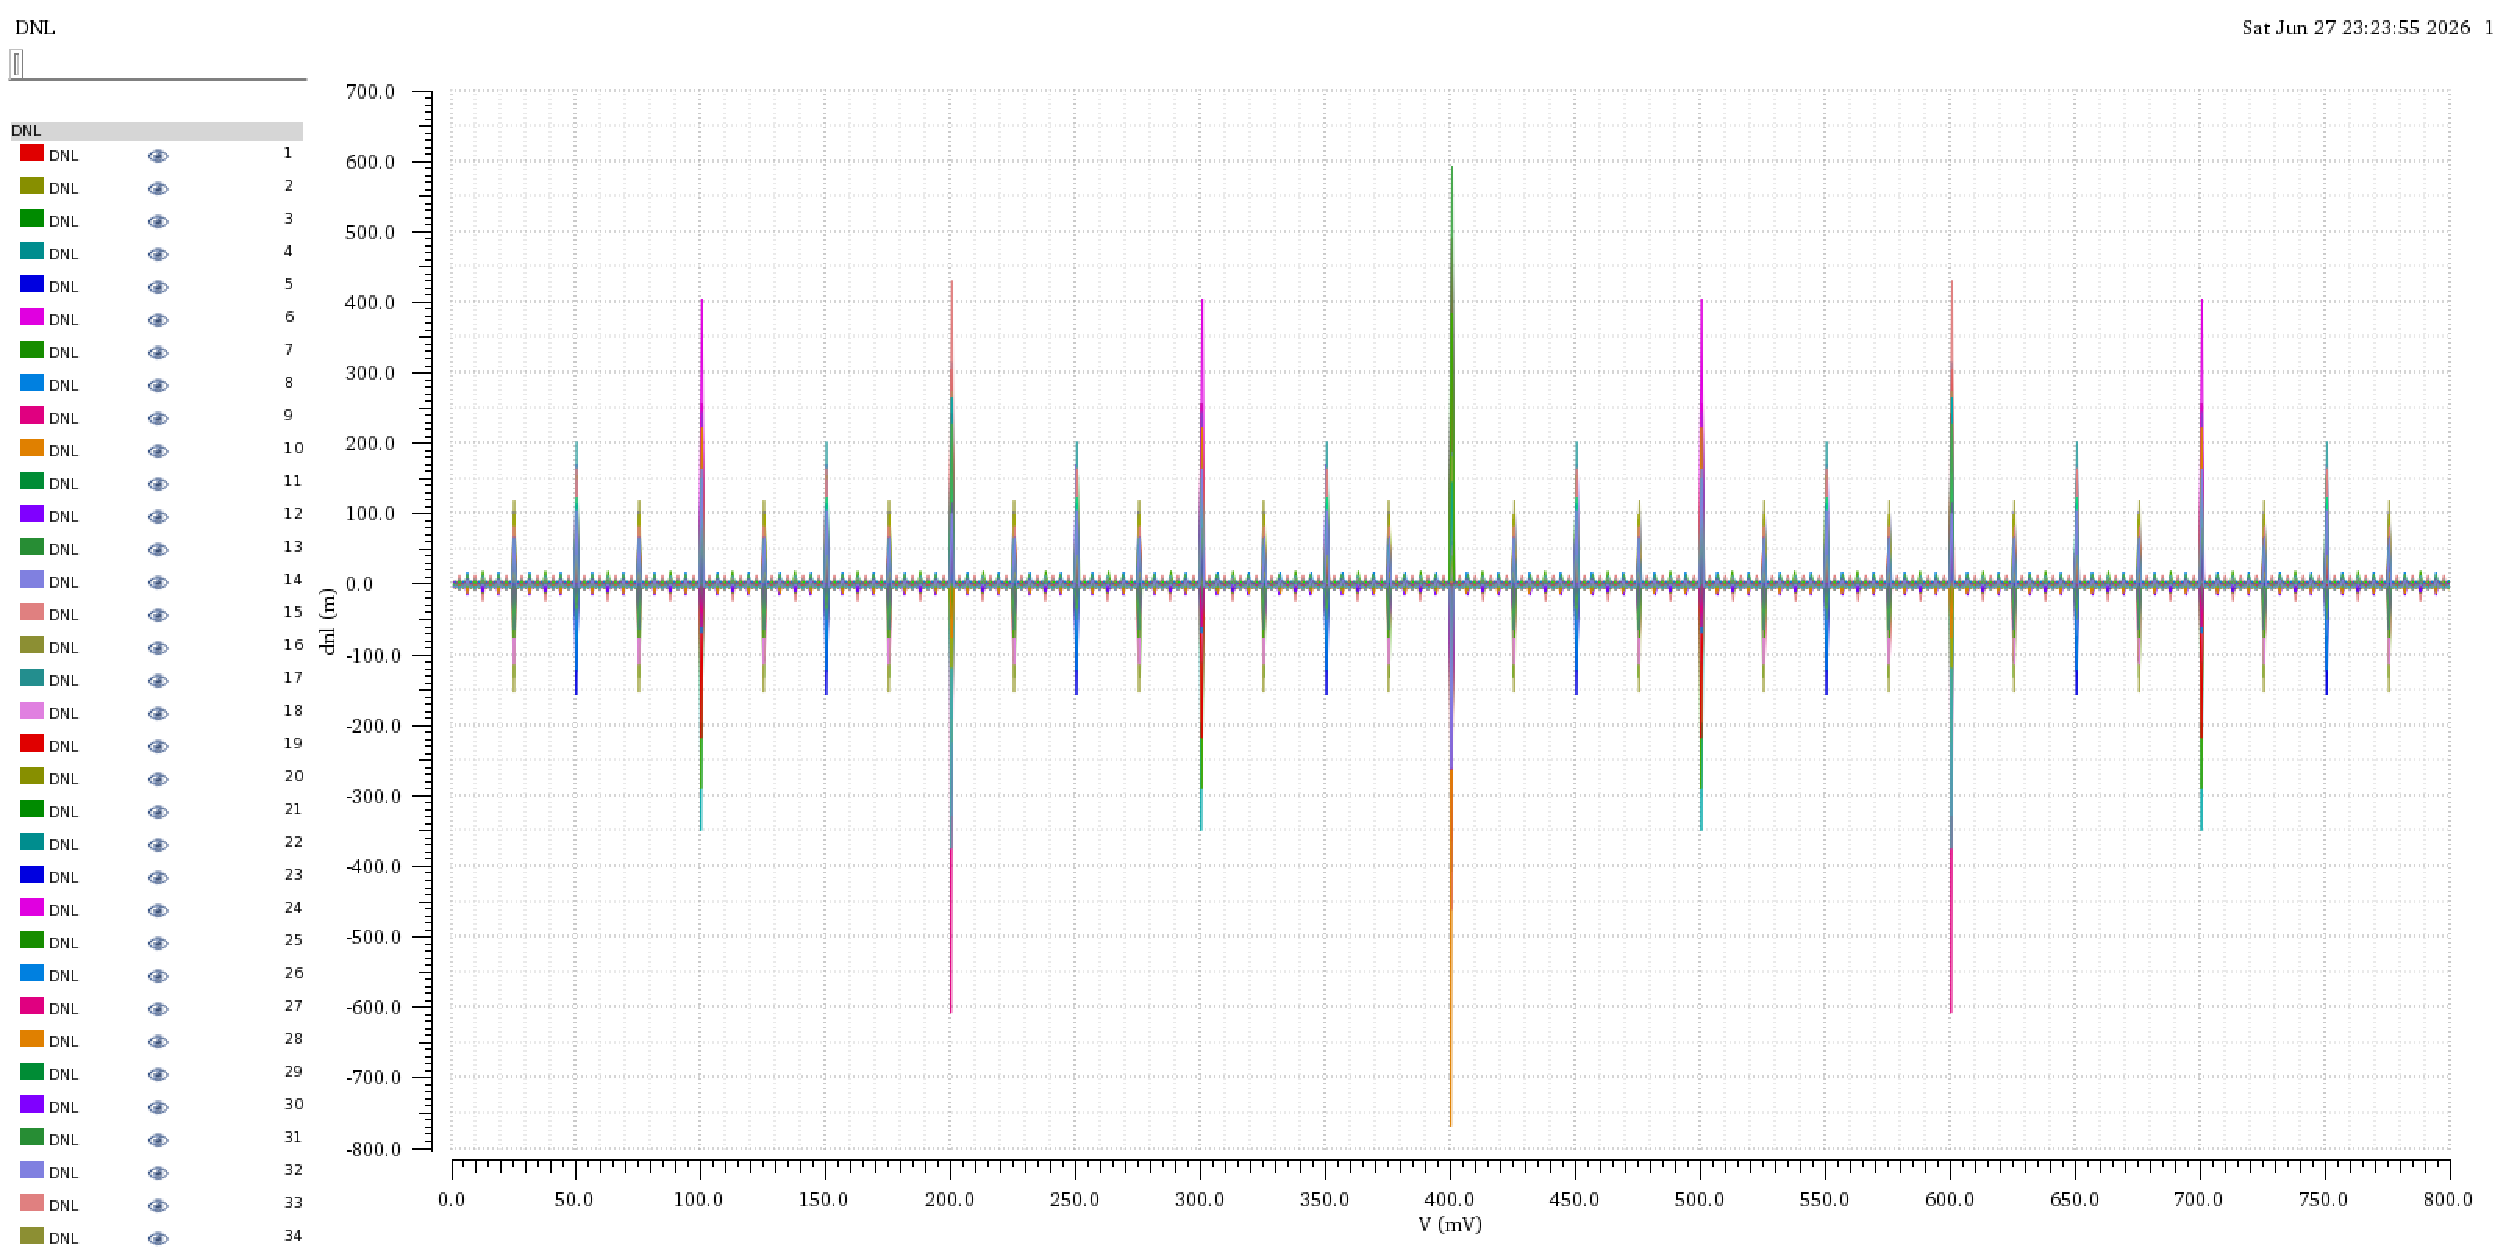
\includegraphics[width=0.8\textwidth]{chapter5/images/5.pdf}
	\caption{DNL for all samples of the bridged cap}
	\label{fig:dnl_samples}
\end{figure}

From Fig.~\ref{fig:dnl_stats}, the area $10\,\mu\mathrm{m} \times 15\,\mu\mathrm{m}$,
corresponding to a capacitance of \SI{35}{fF}, achieved the required standard deviation of the
DNL (137\,mLSB). Therefore, that value was used for the capacitor array.

\subsection*{Bottom Plate Switch Design and Simulation}

The bottom plate switch design should be carefully chosen. The devices used in the switch were
super low-$V_T$ devices, which provide high-speed switching due to their lower on-resistance.
The only issue with those devices is their high leakage current when off, which may affect
operation during the hold phase. Therefore, the size must be chosen carefully to achieve low
on-resistance and a relatively high off-resistance.

\begin{table}[h!]
	\centering
	\caption{Bottom plate switch device parameters}
	\label{tab:devices}
	\begin{tabular}{llllll}
		\toprule
		\textbf{Device} & \textbf{Type} & \textbf{Role} & \textbf{W} & \textbf{L} &
		\textbf{Mul} \\
		\midrule
		Mn0 & SLVTNFET & Input switch       & \SI{7}{\micro m}    & 20\,nm & 4 \\
		Mp0 & SLVTPFET & Input switch       & \SI{7}{\micro m}    & 20\,nm & 4 \\
		Mn1 & SLVTNFET & Digital bit switch & \SI{5.12}{\micro m} & 20\,nm & 2 \\
		Mp1 & SLVTPFET & Digital bit switch & \SI{5.12}{\micro m} & 20\,nm & 2 \\
		\bottomrule
	\end{tabular}
\end{table}

\begin{figure}[h!]
	\centering
	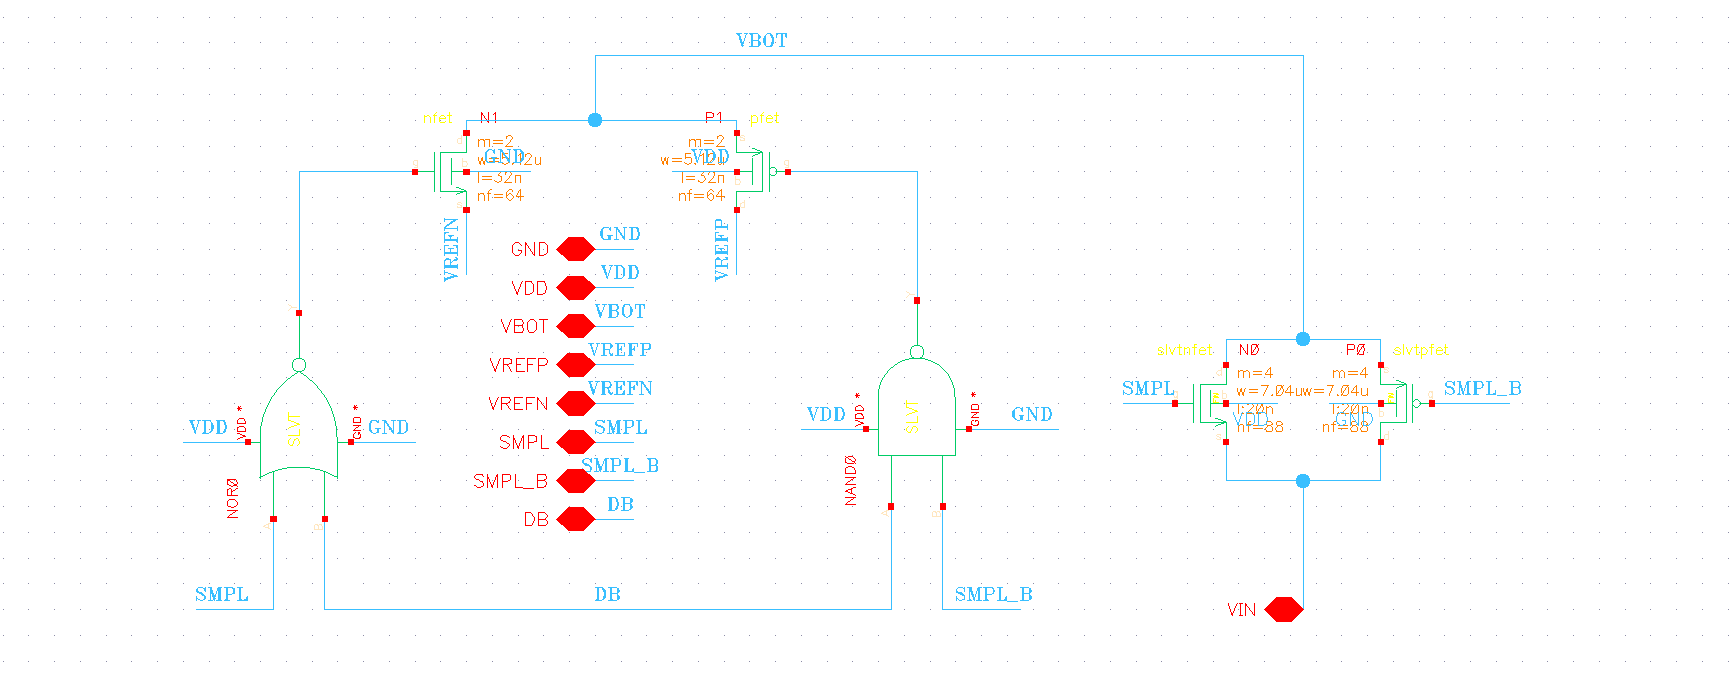
\includegraphics[width=0.8\textwidth]{chapter5/images/6.png}
	\caption{Schematic of the bottom plate switch}
	\label{fig:switch_schematic}
\end{figure}

\subsection*{Testing and Simulation}

\begin{figure}[h!]
	\centering
	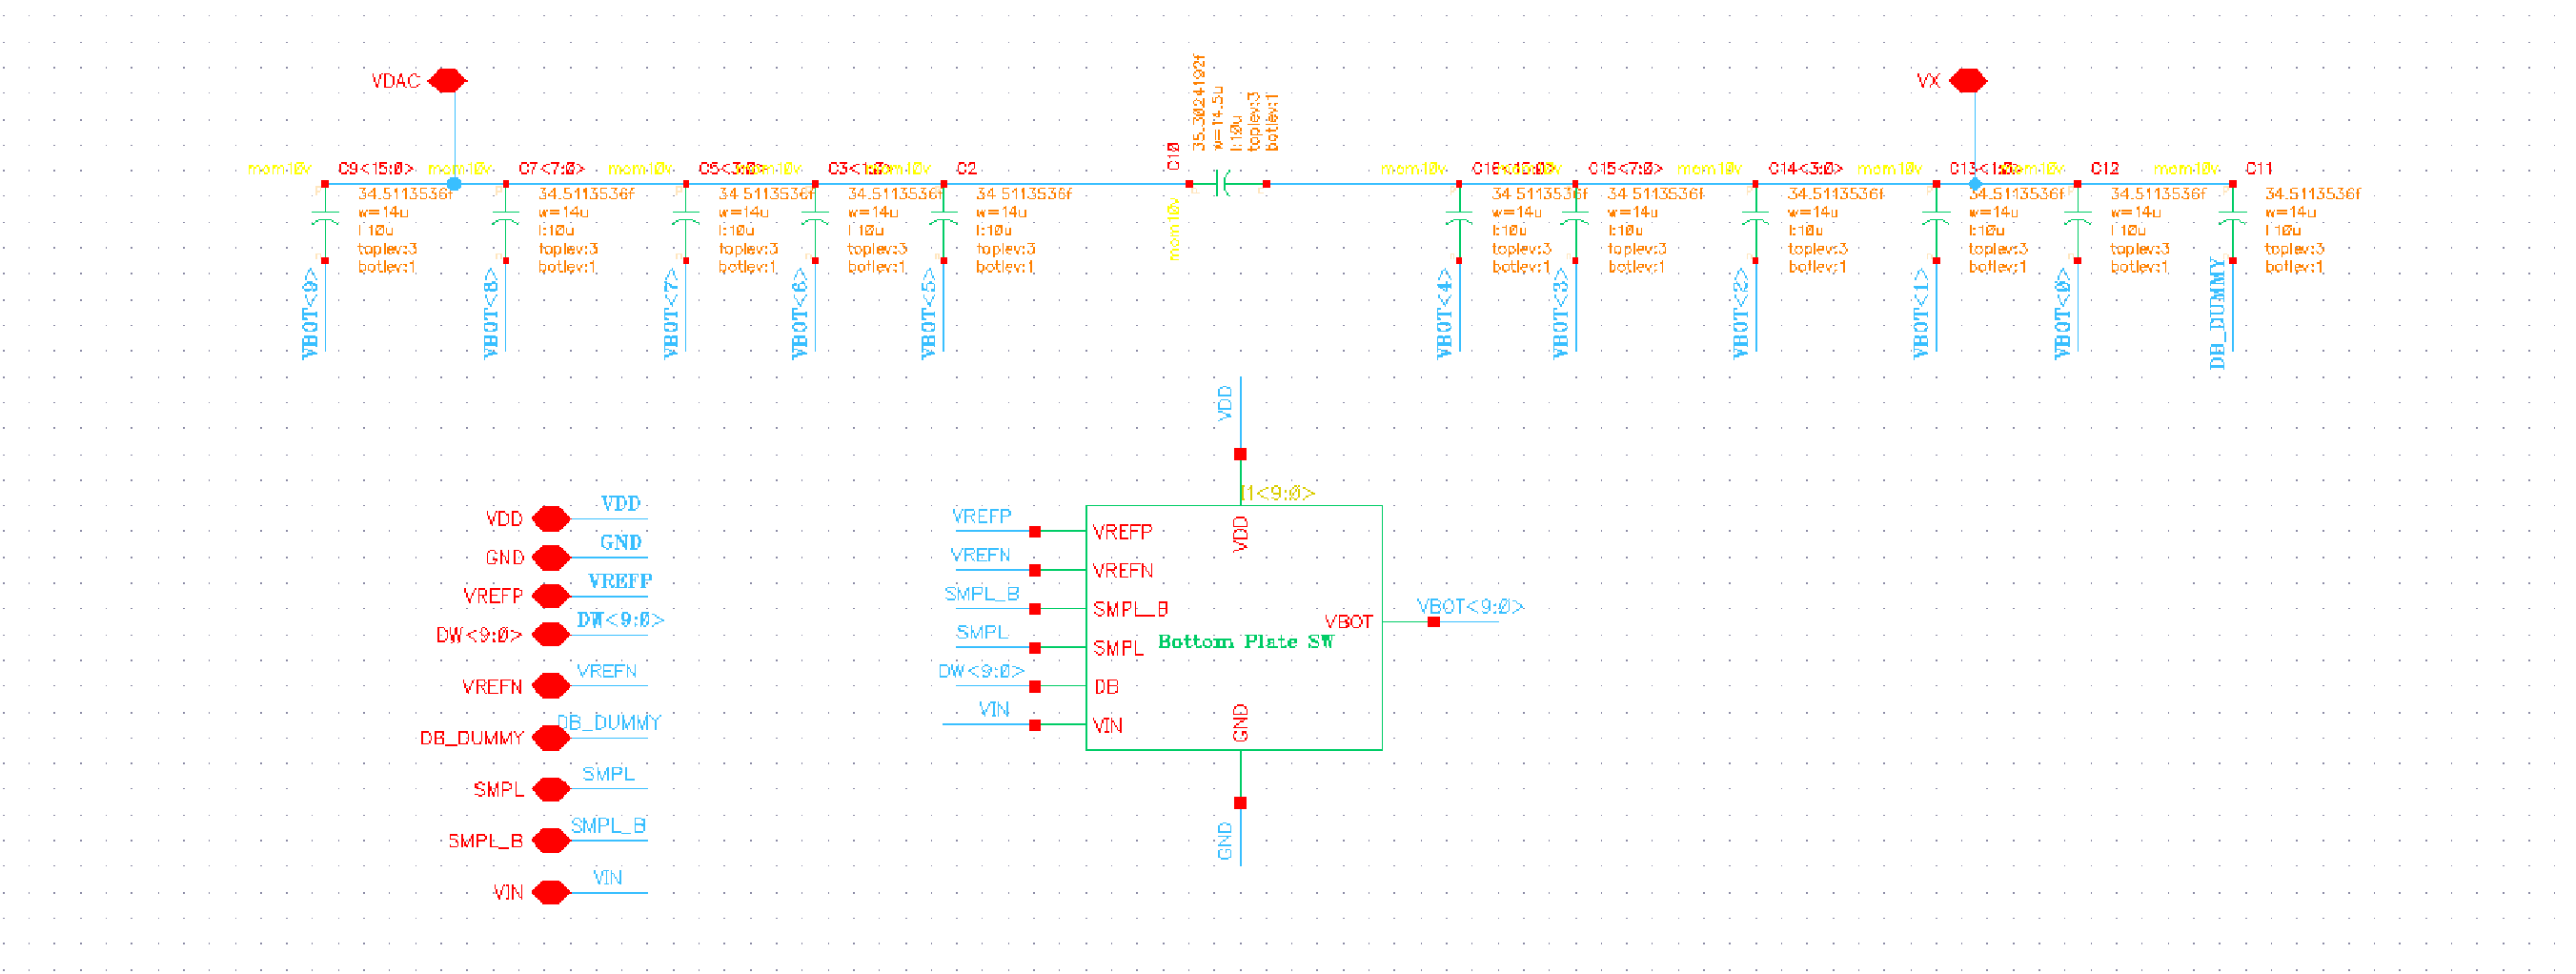
\includegraphics[width=0.8\textwidth]{chapter5/images/7.pdf}
	\caption{Schematic of the bottom plate switch}
	\label{fig:switch_schematic2}
\end{figure}

\begin{figure}[h!]
	\centering
	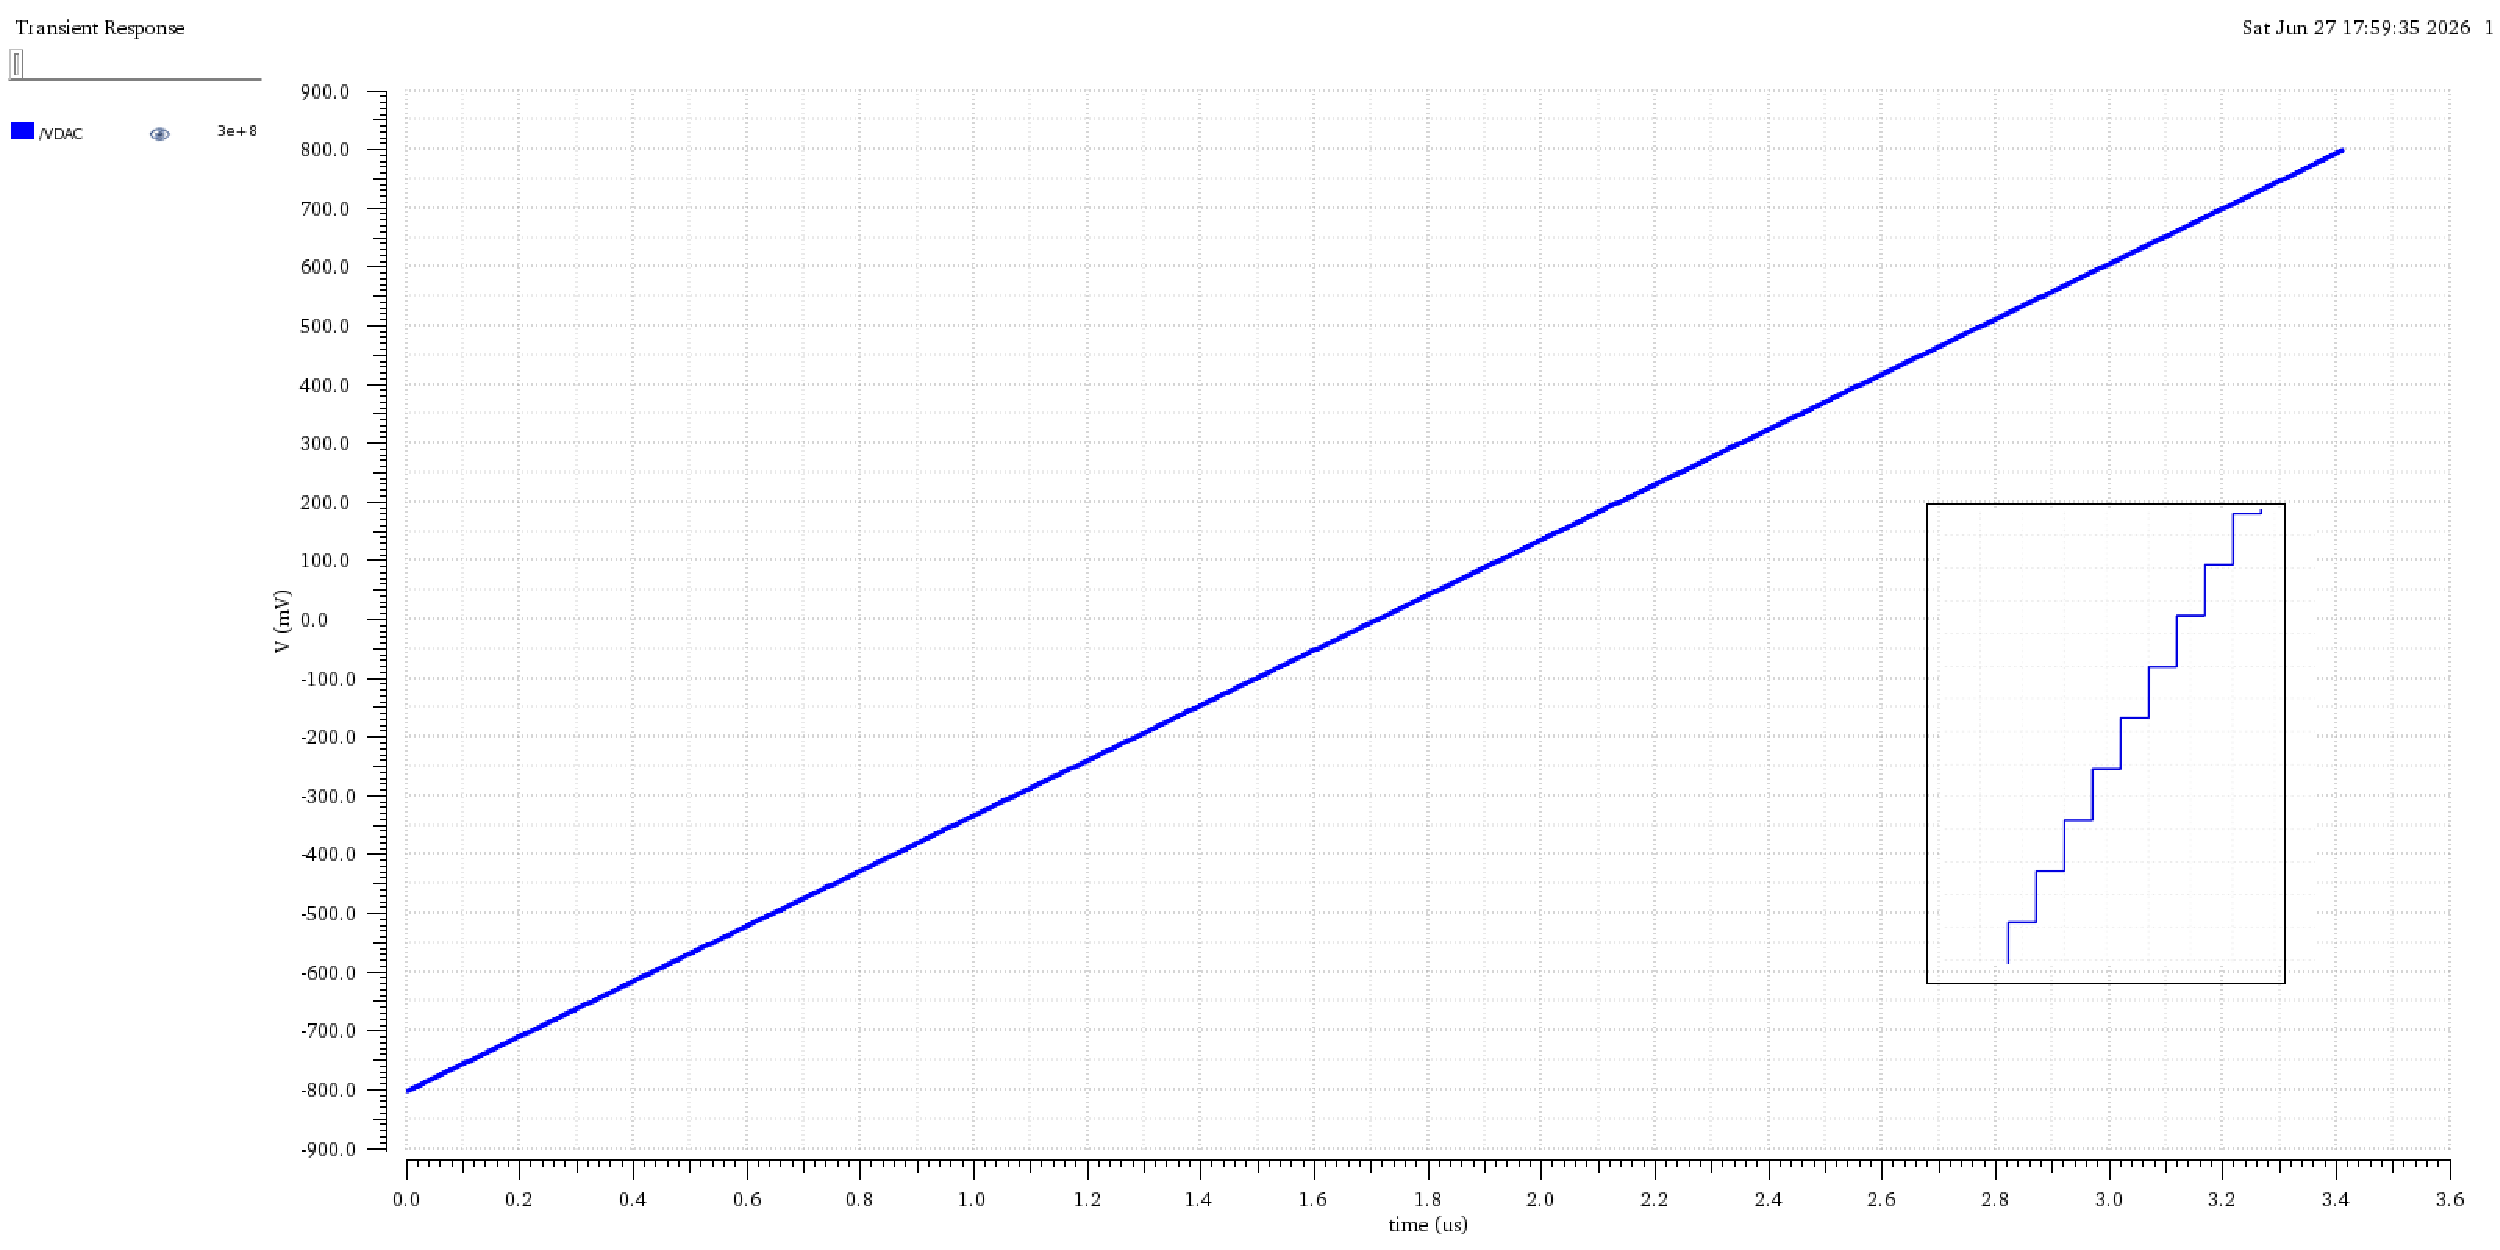
\includegraphics[width=0.8\textwidth]{chapter5/images/8.pdf}
	\caption{Input ramp test for the CDAC}
	\label{fig:ramp_test}
\end{figure}

From Fig.~\ref{fig:ramp_test}, the operation of the CDAC is correct. It captures the full range
from $-800\,\mathrm{mV}$ to $+800\,\mathrm{mV}$, which is the peak-to-peak signal that will be
entered into the ADC.
\newpage
\section{Asynchronous Clock Generator: Design and Simulation}
\label{sec:async_clk_gen_design}

This section presents the transistor-level implementation of the
asynchronous internal clock generator introduced in
Section~\ref{sec:async_clk_gen}, including the set/reset D flip-flop and
the 2-to-1 multiplexer cells used to construct it, along with the device
sizing for each building block.

\subsection{Top-Level Schematic}

The complete gate-level implementation of the clock generator is shown in
Fig.~\ref{fig:clkgen_schematic}, matching the architecture described in
Section~\ref{sec:async_clk_gen}.

\begin{figure}[h]
	\centering
	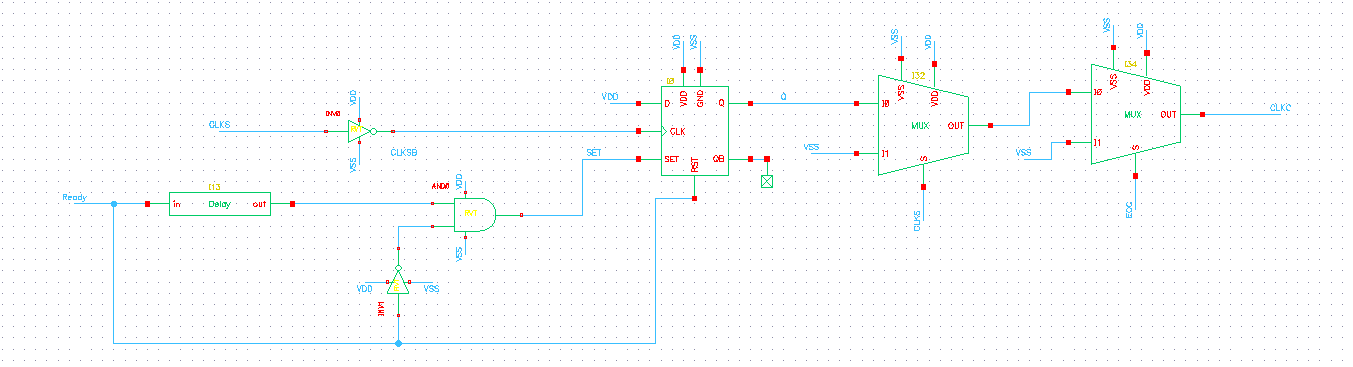
\includegraphics[width=0.95\textwidth]{chapter5/images/CLK/sch.png}
	\caption{Transistor/gate-level schematic of the asynchronous internal
		clock generator.}
	\label{fig:clkgen_schematic}
\end{figure}

\subsection{2-to-1 Multiplexer}

Each multiplexer is implemented using two CMOS transmission gates and a
single inverter, as shown in Fig.~\ref{fig:mux_schematic}. The inverter
generates the complementary select signal so that exactly one
transmission gate is enabled at a time: when $S = 0$, \texttt{XGATE0}
passes $I0$ to the output; when $S = 1$, \texttt{XGATE1} passes $I1$ to
the output.

\begin{figure}[h]
	\centering
	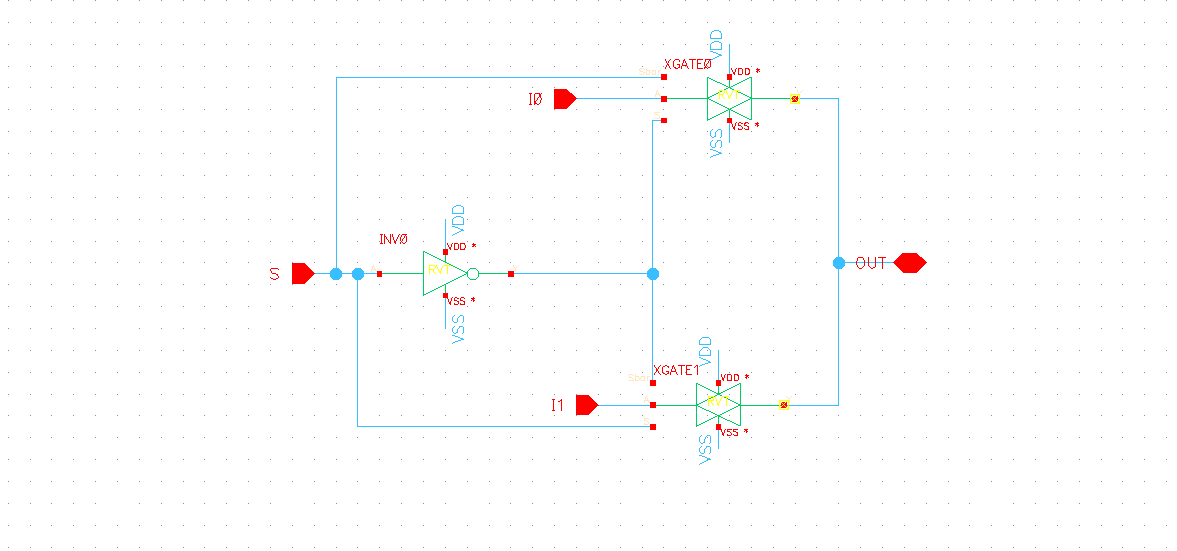
\includegraphics[width=0.75\textwidth]{chapter5/images/CLK/mux.png}
	\caption{2-to-1 multiplexer schematic, implemented with two
		transmission gates and an inverter.}
	\label{fig:mux_schematic}
\end{figure}

\subsection{Set/Reset D Flip-Flop}

The set/reset DFF used in the clock generator is implemented as a static
CMOS master-slave latch with dedicated active-high set and reset pull-up
and pull-down devices, as shown in Fig.~\ref{fig:dff_schematic}. As noted
in Section~\ref{sec:async_clk_gen}, both $SET$ and $RST$ are active-high
in this design.

\begin{figure}[h]
	\centering
	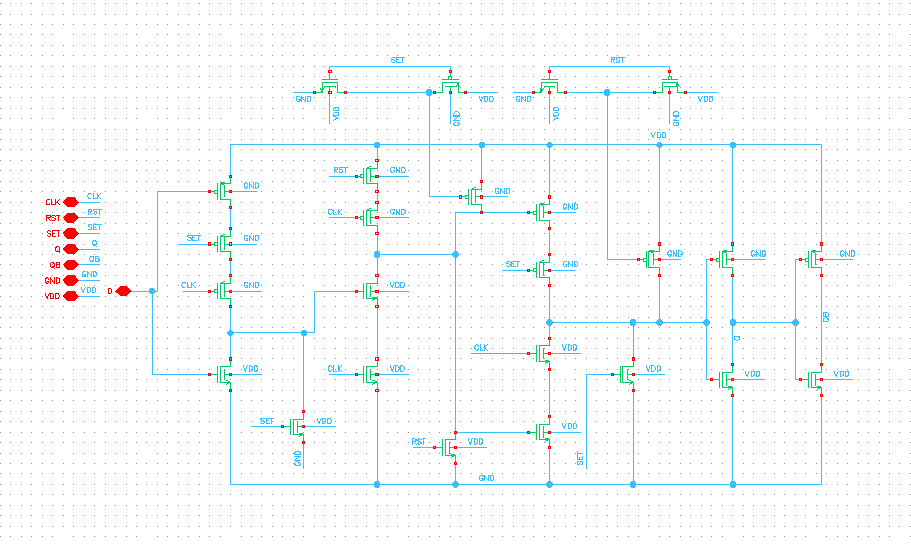
\includegraphics[width=0.85\textwidth]{chapter5/images/CLK/DFF.png}
	\caption{Transistor-level schematic of the set/reset D flip-flop.}
	\label{fig:dff_schematic}
\end{figure}
\newpage
\subsection{Device Sizing}
Table~\ref{tab:clkgen_sizing} summarizes the transistor sizing used for
the transmission gates in the multiplexer and for all transistors in the
flip-flop.The transmission gates are sized significantly wider than the
flip-flop's internal devices to minimize the on-resistance of the
multiplexer's signal path, since the multiplexer output, $CLKC$, must
drive the comparator's clock input with minimal added delay.

\begin{table}[h]
	\centering
	\caption{Transistors Sizing of Asynchronous Clock Generator.}
	\label{tab:clkgen_sizing}
	\begin{tabular}{@{}llcc@{}}
		\toprule
		Block & Device Type & $W$ & $L$ \\
		\midrule
		Mux transmission gate (\texttt{XGATE0}, \texttt{XGATE1}) & NMOS (slvt) & $24\,\mu\text{m}$ & $20\,\text{nm}$ \\
		Mux transmission gate (\texttt{XGATE0}, \texttt{XGATE1}) & PMOS (slvt) & $24\,\mu\text{m}$ & $20\,\text{nm}$ \\
		\midrule
		D flip-flop & NMOS (rlvt) & $8\,\mu\text{m}$   & $20\,\text{nm}$ \\
		D flip-flop & PMOS (rlvt) & $6.4\,\mu\text{m}$ & $20\,\text{nm}$ \\
		\midrule
		Inverters - AND gate & NMOS (slvt) & $24\,\mu\text{m}$   & $20\,\text{nm}$ \\
		Inverters - AND gate & PMOS (slvt) & $24\,\mu\text{m}$   & $20\,\text{nm}$ \\
		\bottomrule
	\end{tabular}
\end{table}
\subsection{Functional Verification}
\label{sec:clkgen_functional_verification}

To verify the complete self-timed handshake behavior of the asynchronous
clock generator, a transient simulation was performed with the full
signal chain: the external sampling clock ($CLKS$), the generated
internal clock ($CLKC$), the comparator's $Ready$ signal, the flip-flop's
internal set pulse ($SET$), and the end-of-conversion signal ($EOC$). The
resulting waveforms, spanning two complete sample-and-convert cycles, are
shown in Fig.~\ref{fig:clkgen_transient}.

\begin{figure}[h]
	\centering
	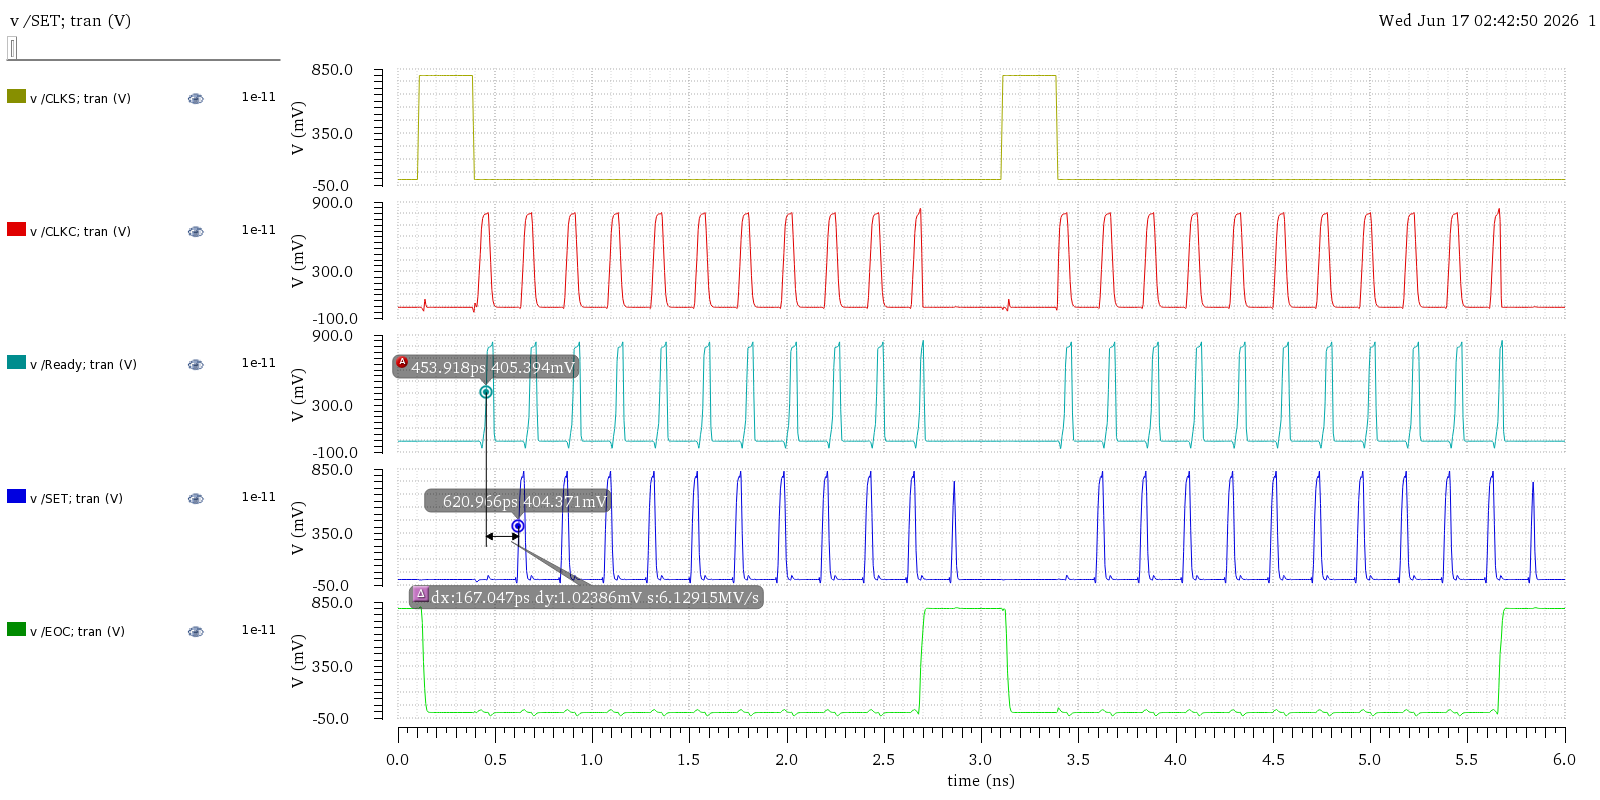
\includegraphics[width=0.95\textwidth]{chapter5/images/CLK/Signals.png}
	\caption{Transient simulation of the asynchronous clock generator,
		showing $CLKS$, $CLKC$, $Ready$, $SET$, and $EOC$.}
	\label{fig:clkgen_transient}
\end{figure}

The waveforms confirm the expected self-timed operation described in
Section~\ref{sec:async_clk_gen}.as marked by the cursors in
Fig.~\ref{fig:clkgen_transient}: the $Ready$ pulse occurs at
$453.92\,\text{ps}$ and the resulting $SET$ pulse occurs at
$620.96\,\text{ps}$, giving a measured delay of
$167.05\,\text{ps}$. This delay from delay cell = $150 ,\ psec$ and propagation delay of circuits this directly sets the low period of CLKC clock.

\section{DAC Reference Buffer: Design and Simulation}
\label{sec:vref_buffer_design}

This section presents the transistor-level implementation of the
reference buffer introduced in Section~\ref{sec:vref_buffer}. The
complete schematic, including device sizing for the error amplifier, bias
mirror, and PMOS pass transistor, is shown in
Fig.~\ref{fig:vref_buffer_full_schematic}.

\begin{figure}[h]
	\centering
	
\includegraphics[width=0.85\textwidth]{chapter5/images/LDO/sch.png}
	\caption{Transistor-level schematic of the DAC reference buffer.}
	\label{fig:vref_buffer_full_schematic}
\end{figure}

The circuit consists of a NMOS-input differential pair (\texttt{NO},
\texttt{N1}) loaded by an NMOS current mirror (\texttt{P0}, \texttt{P1}),
biased by a tail current source (\texttt{N4}) and a bias-mirror reference
branch (\texttt{N6}, biased by the ideal current source \texttt{I41}).
The amplifier's output, $V_M$, drives the gate of the PMOS pass
transistor \texttt{P8}, which delivers the regulated output current to
the $Output$ node. An additional NMOS device, \texttt{N5}, biased from
the same bias-mirror network, provides the output-stage biasing/loading
required to set the buffer's quiescent operating point. The output node
is loaded by the reference decoupling capacitor, $C1 = 2 \, nF $ (corresponding to
$C_{ref}$ in Section~\ref{sec:vref_bounce}).

Table~\ref{tab:vref_buffer_sizing} lists the width ($W$), length ($L$),
and multiplier ($m$) of every transistor in the design, as configured in
the schematic.

\begin{table}[h]
	\centering
	\caption{Transistor sizing for the DAC reference buffer.}
	\label{tab:vref_buffer_sizing}
	\begin{tabular}{@{}llrrr@{}}
		\toprule
		Device & Type & $W$ & $L$ & $m$ \\
		\midrule
		$P1$ & PMOS & $2.88\,\mu\text{m}$  & $80\,\text{nm}$  & 3   \\
		$P0$ & PMOS & $2.88\,\mu\text{m}$  & $80\,\text{nm}$  & 3   \\
		$N0$ & NMOS & $2\,\mu\text{m}$     & $80\,\text{nm}$  & 3   \\
		$N1$ & NMOS & $2\,\mu\text{m}$     & $80\,\text{nm}$  & 3   \\
		$N4$ & NMOS & $1.68\,\mu\text{m}$  & $80\,\text{nm}$  & 3   \\
		$N6$ & NMOS & $1.68\,\mu\text{m}$  & $80\,\text{nm}$  & 3   \\
		$N5$ & NMOS & $59.84\,\mu\text{m}$ & $120\,\text{nm}$ & 120 \\
		$P8$ & PMOS (pass transistor) & $68\,\mu\text{m}$ & $80\,\text{nm}$ & 210 \\
		\bottomrule
	\end{tabular}
\end{table}

\noindent The bias current source \texttt{I41} sets a reference current
of $44\,\mu\text{A}$, which is mirrored through \texttt{N6} and
\texttt{N4} to bias the amplifier's tail and output stage. The pass
transistor \texttt{P8} is sized substantially larger than the amplifier
devices, both to supply the output current required by the load and to
minimize the buffer's output impedance, $R_{out}$, which, together with
$C_{ref}$, sets the bounce recovery time constant derived in
Section~\ref{sec:vref_bounce}.

\subsection{DC Operating Point}
\label{sec:vref_buffer_dcop}

To verify that every transistor in the reference buffer is biased
correctly at its intended operating point, a DC operating-point
simulation was performed. The annotated schematic, showing the drain
current, threshold voltage, terminal voltages, and small-signal
parameters for each device, is shown in
Fig.~\ref{fig:vref_buffer_dcop_schematic}.

\begin{figure}[h]
	\centering
	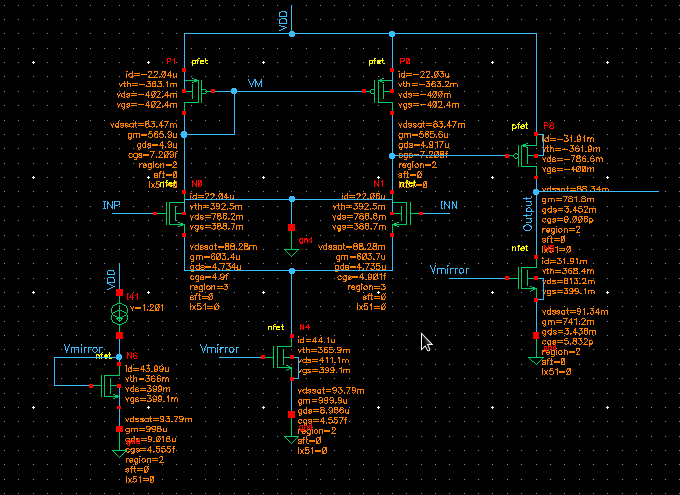
\includegraphics[width=0.95\textwidth]{chapter5/images/LDO/DCop.png}
	\caption{DC operating-point annotation for the DAC reference buffer.}
	\label{fig:vref_buffer_dcop_schematic}
\end{figure}

Table~\ref{tab:vref_buffer_dcop} summarizes the key DC operating-point
parameters extracted for each transistor: drain current ($I_D$),
threshold voltage ($V_{th}$), drain-source voltage ($V_{ds}$),
gate-source voltage ($V_{gs}$), overdrive/saturation voltage
($V_{dsat}$), and small-signal transconductance and output conductance
($g_m$, $g_{ds}$).

\begin{table}[h]
	\centering
	\caption{DC operating-point summary for the DAC reference buffer.}
	\label{tab:vref_buffer_dcop}
	\resizebox{\textwidth}{!}{%
		\begin{tabular}{@{}lrrrrrrr@{}}
			\toprule
			Device & $I_D$ & $V_{th}$ & $V_{ds}$ & $V_{gs}$ & $V_{dsat}$ & $g_m$ & $g_{ds}$ \\
			\midrule
			$P1$ & $-22.04\,\mu\text{A}$ & $-383.1\,\text{mV}$ & $-402.4\,\text{mV}$ & $-402.4\,\text{mV}$ & $83.47\,\text{mV}$ & $565.9\,\mu\text{A/V}$ & $4.9\,\mu\text{A/V}$ \\
			$P0$ & $-22.03\,\mu\text{A}$ & $-363.2\,\text{mV}$ & $-400.0\,\text{mV}$ & $-402.4\,\text{mV}$ & $83.47\,\text{mV}$ & $565.6\,\mu\text{A/V}$ & $4.917\,\mu\text{A/V}$ \\
			$N0$ & $22.04\,\mu\text{A}$  & $392.5\,\text{mV}$  & $786.2\,\text{mV}$  & $388.7\,\text{mV}$  & $88.28\,\text{mV}$ & $803.4\,\mu\text{A/V}$ & $4.734\,\mu\text{A/V}$ \\
			$N1$ & $22.06\,\mu\text{A}$  & $392.5\,\text{mV}$  & $788.8\,\text{mV}$  & $388.7\,\text{mV}$  & $88.29\,\text{mV}$ & $803.7\,\mu\text{A/V}$ & $4.735\,\mu\text{A/V}$ \\
			$N6$ & $43.89\,\mu\text{A}$  & $366.0\,\text{mV}$  & $399.0\,\text{mV}$  & $399.1\,\text{mV}$  & $93.79\,\text{mV}$ & $998\,\mu\text{A/V}$ & $9.018\,\mu\text{A/V}$ \\
			$N4$ & $44.1\,\mu\text{A}$   & $365.9\,\text{mV}$  & $411.1\,\text{mV}$  & $399.1\,\text{mV}$  & $93.79\,\text{mV}$ & $999.9\,\mu\text{A/V}$ & $8.986\,\mu\text{A/V}$ \\
			$P8$ (pass) & $-31.91\,\text{mA}$ & $-361.0\,\text{mV}$ & $-786.6\,\text{mV}$ & $-400\,\text{mV}$ & $88.34\,\text{mV}$ & $781.8\,\text{mA/V}$ & $3.452\,\text{mA/V}$ \\
			$N5$ & $31.91\,\text{mA}$ & $368.4\,\text{mV}$ & $813.2\,\text{mV}$ & $399.1\,\text{mV}$ & $91.34\,\text{mV}$ & $741.2\,\text{mA/V}$ & $3.438\,\text{mA/V}$ \\
			\bottomrule
	\end{tabular}}
\end{table}

\subsection{Open-Loop Gain and Stability}
\label{sec:vref_buffer_loop_gain}
To verify the stability of the negative-feedback regulation loop, the
open-loop (loop) gain of the reference buffer was simulated across
frequency. The resulting Bode plot is shown in
Fig.~\ref{fig:vref_buffer_loop_gain}.


\begin{figure}[h]
	\centering
	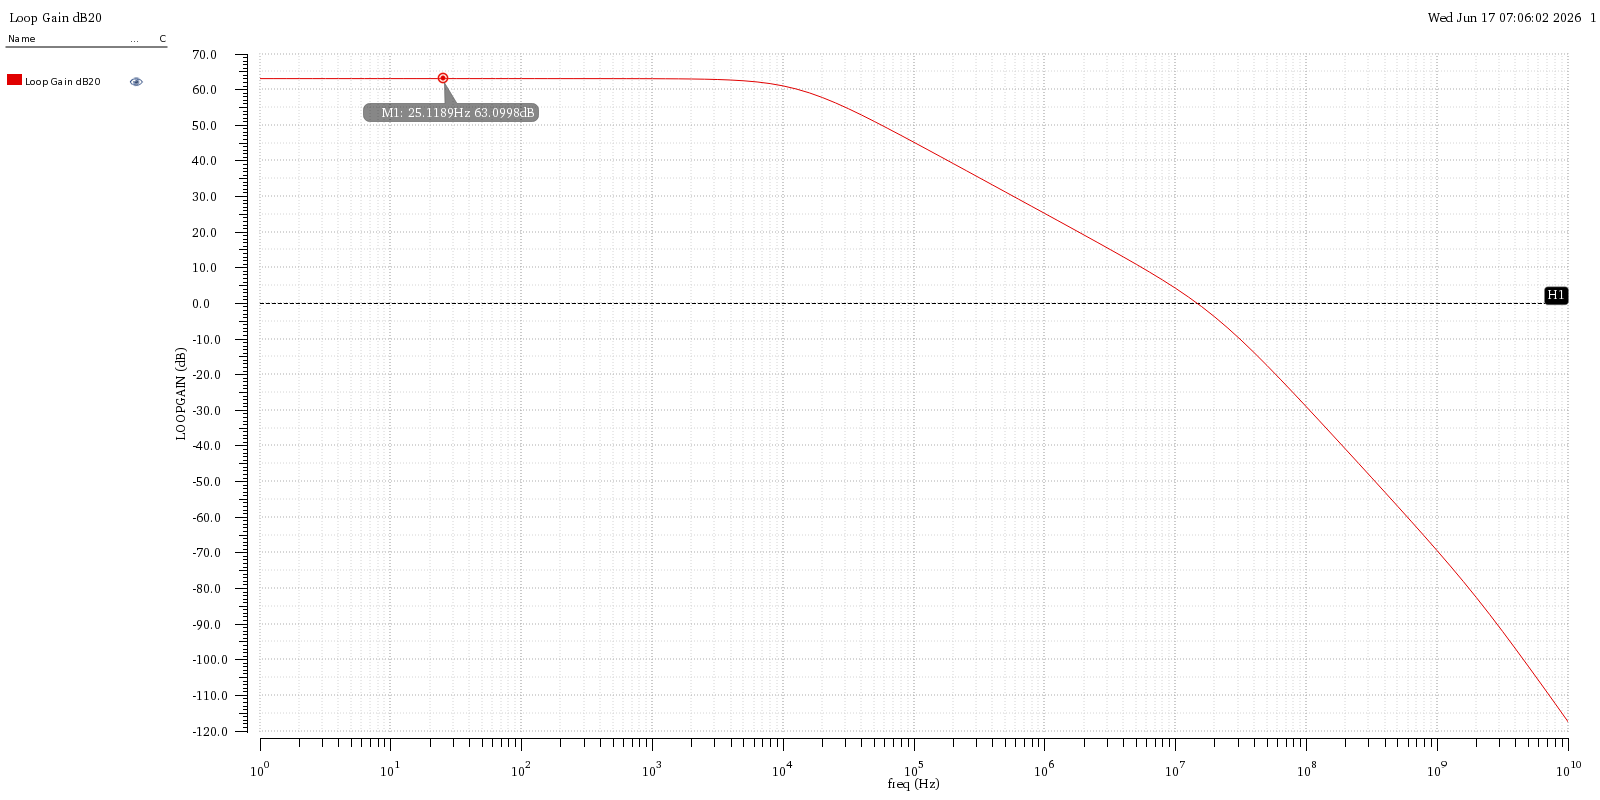
\includegraphics[width=0.85\textwidth]{chapter5/images/LDO/OL.png}
	\caption{Simulated open-loop gain of the DAC reference buffer.}
	\label{fig:vref_buffer_loop_gain}
\end{figure}
The simulated DC loop gain is $63.10\,\text{dB}$, providing approximately
$1430\times$ of low-frequency loop gain to suppress the steady-state
error between $V_{out}$ and $V_{REF}$. The loop gain rolls off at
$-20\,\text{dB/decade}$ from the dominant pole and crosses unity gain
(\text{0\,dB}) at a unity-gain frequency (UGF) of approximately
$15\,\text{MHz}$. This UGF sets the bandwidth over which the buffer can
actively correct the reference voltage bounce caused by DAC switching
events (Section~\ref{sec:vref_bounce}), and is therefore directly tied to
the buffer's ability to recover from a switching transient within the
required settling time.
\newpage
\subsection{Phase Margin vs.\ Load Current}
\label{sec:vref_buffer_pm_vs_iload}

Since the reference buffer must remain stable across its full range of
output loading, from no load up to the maximum current the DAC array can
draw during a switching event, the loop's phase margin was simulated
while sweeping the output load current, $I_{load}$, from $0$ to
$30\,\text{mA}$, matching the worst-case current delivered by the pass
transistor identified in the DC operating-point analysis of
Section~\ref{sec:vref_buffer_dcop}. The resulting phase margin
characteristic is shown in Fig.~\ref{fig:vref_buffer_pm_vs_iload}.

\begin{figure}[h]
	\centering
	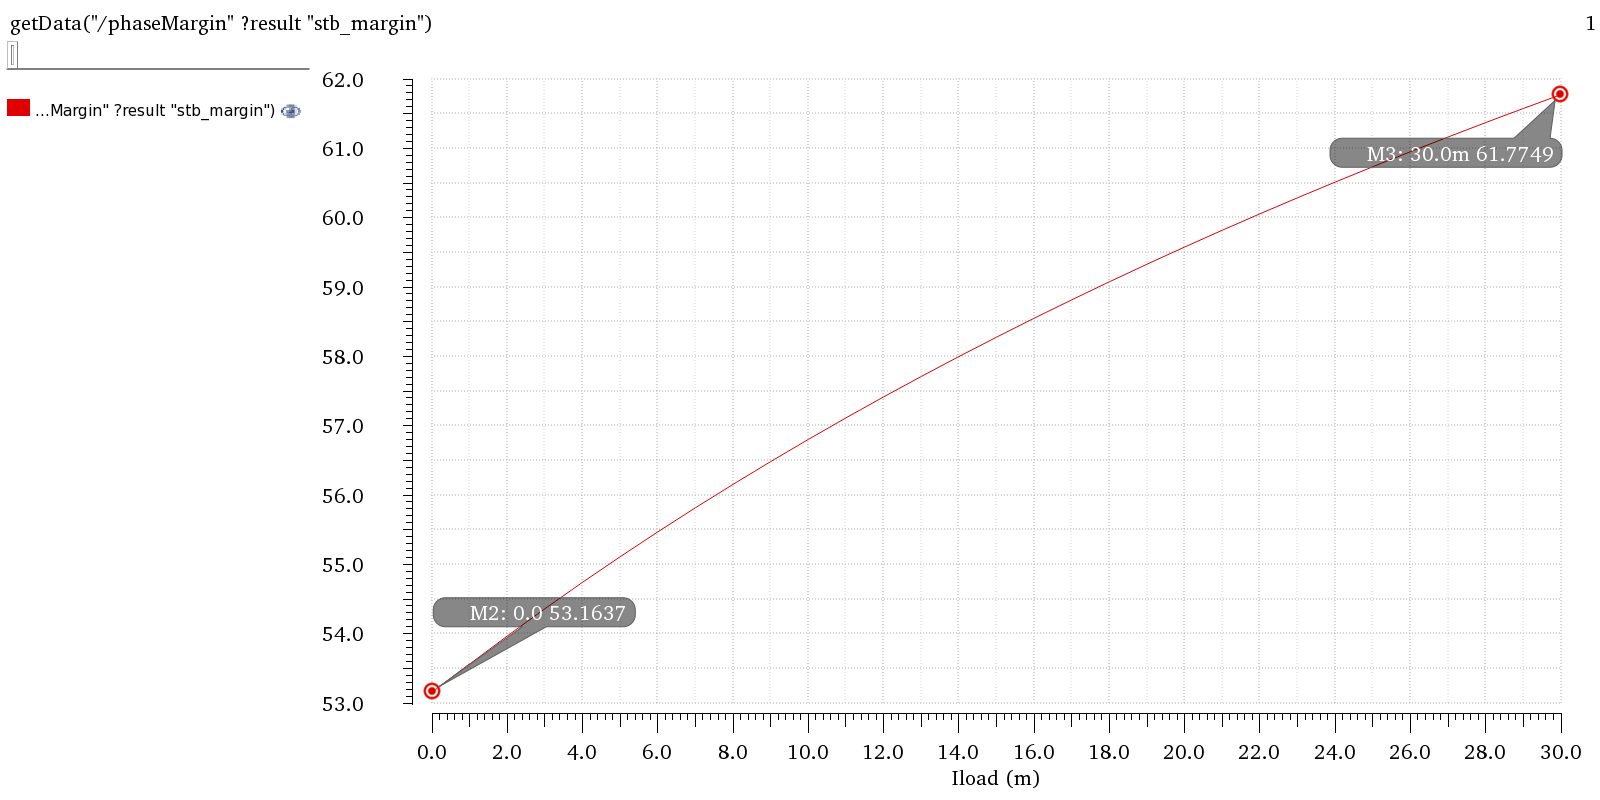
\includegraphics[width=0.85\textwidth]{chapter5/images/LDO/PM.png}
	\caption{Simulated phase margin of the DAC reference buffer as a
		function of output load current.}
	\label{fig:vref_buffer_pm_vs_iload}
\end{figure}

The phase margin increases monotonically with load current, from
$53.16^\circ$ at no load ($I_{load} = 0\,\text{mA}$) to $61.77^\circ$ at
the maximum simulated load ($I_{load} = 30\,\text{mA}$). Across the
entire swept range, the phase margin remains comfortably above the
standard $45^\circ$ stability criterion, confirming that the reference
buffer remains stable under all loading conditions expected during
normal operation of the DAC, including the worst-case transient current
demanded immediately after a switching event.

\subsection{Transient Load-Step Response}
\label{sec:vref_buffer_load_transient}

To verify the reference buffer's dynamic response under the same
worst-case loading condition used in the stability analysis of
Section~\ref{sec:vref_buffer_pm_vs_iload}, a transient simulation was
performed in which a $30\,\text{mA}$ output current pulse, with a
$30\,\text{ps}$ edge rate, is applied to the buffer's output node. The
resulting settling behavior of $V_{out}$ is shown in
Fig.~\ref{fig:vref_buffer_load_transient}.

\begin{figure}[h]
	\centering
	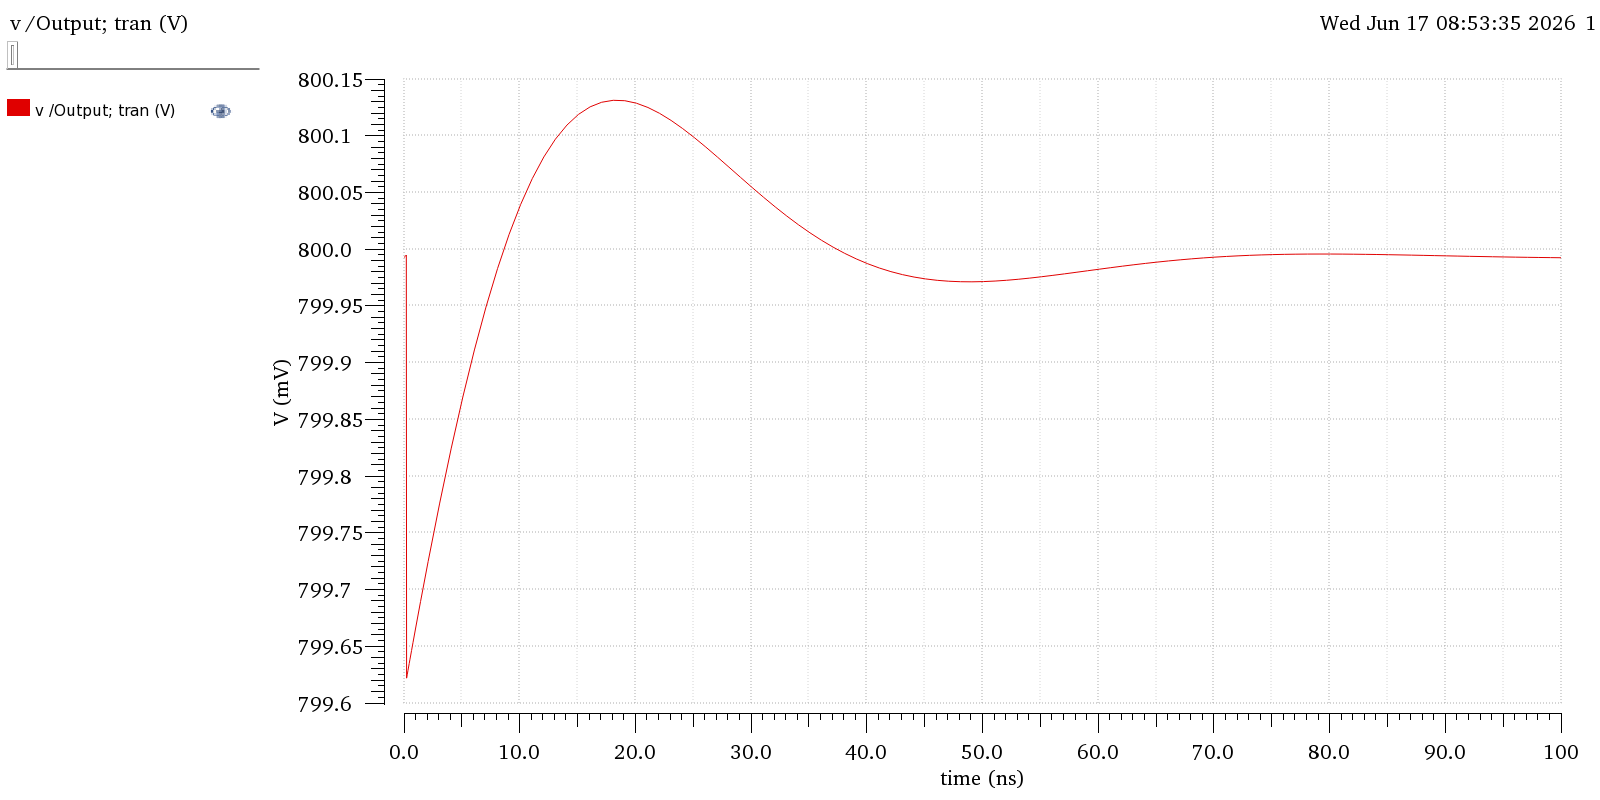
\includegraphics[width=0.85\textwidth]{chapter5/images/LDO/TS2.png}
	\caption{Transient response of the reference buffer output to a
		$30\,\text{mA}$ load current pulse with a $30\,\text{ps}$ width.}
	\label{fig:vref_buffer_load_transient}
\end{figure}

In response to the abrupt load step, $V_{out}$ initially droops by
approximately $0.38\,\text{mV}$ before the feedback loop reacts and
drives the output back toward its nominal value. Consistent with the
moderate ($53^\circ$ to $62^\circ$) phase margin measured in
Section~\ref{sec:vref_buffer_pm_vs_iload}, the response is underdamped:
$V_{out}$ overshoots the final value by approximately $0.13\,\text{mV}$
before settling into a lightly damped oscillation that decays within
approximately $70 \,\text{ns}$.
\subsubsection{Transient Settling Across Process and Temperature Corners}
\label{sec:vref_buffer_settling_corners}

To verify that the reference buffer recovers from a load-step transient
within the required system settling budget across the
full range of manufacturing and environmental variation, the load-step
settling test from Section~\ref{sec:vref_buffer_load_transient} was
re-simulated at the SS corner ($125^\circ\text{C}$, $-5\%\,V_{DD}$) and
the FF corner ($-40^\circ\text{C}$, $+5\%\,V_{DD}$), in addition to the
nominal (typical) corner. The same $30\,\text{mA}$ load current pulse
used in the nominal-corner simulation was applied at each corner. The
resulting settling waveforms are shown in
Fig.~\ref{fig:vref_buffer_settling_corners}.

\begin{figure}[h]
	\centering
	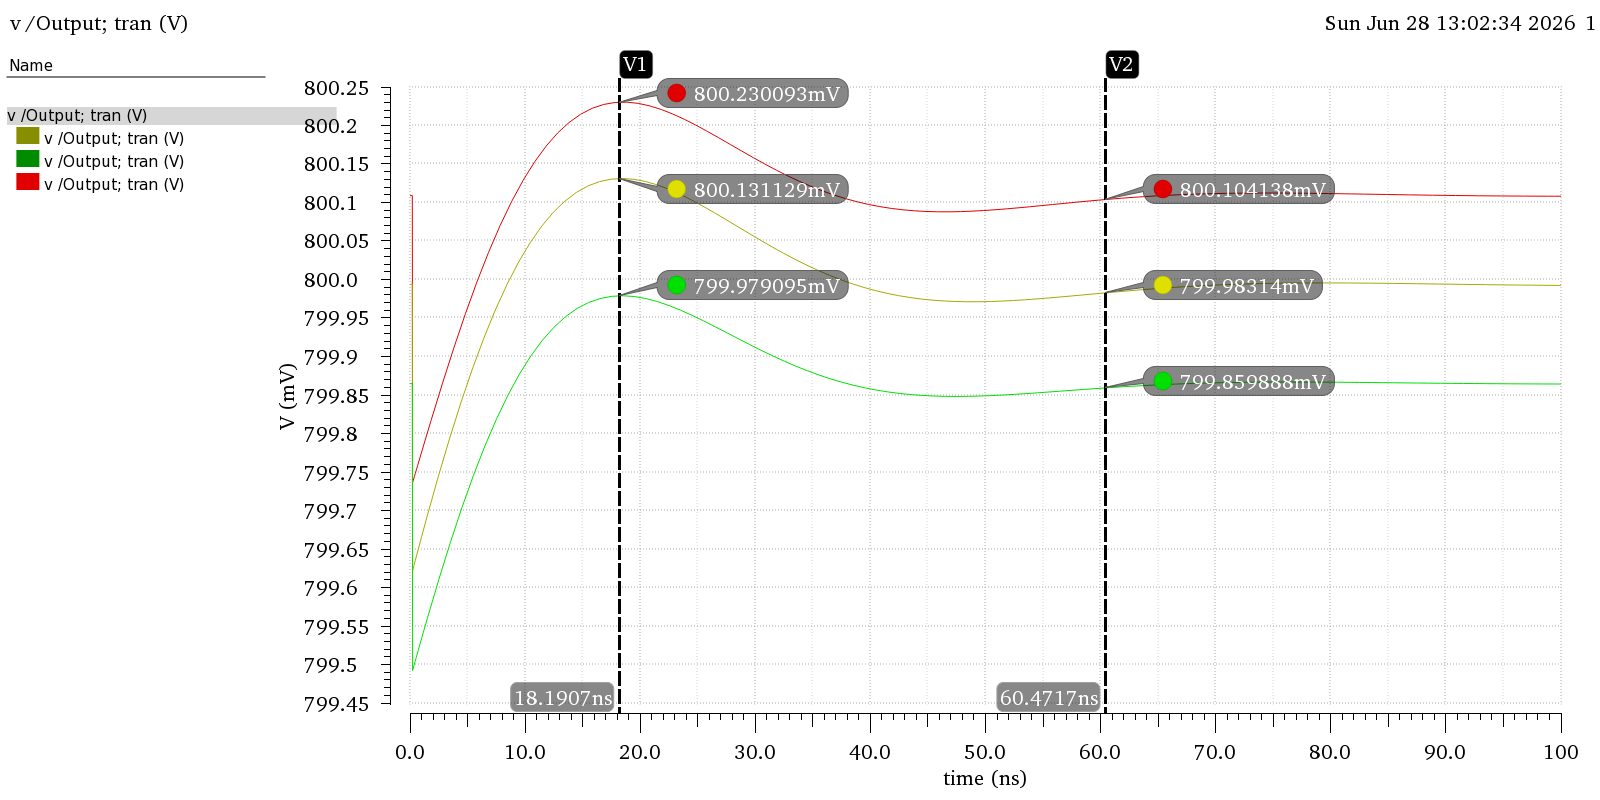
\includegraphics[width=0.95\textwidth]{chapter5/images/LDO/co.png}
	\caption{Transient load-step settling response of the reference
		buffer at the SS ($125^\circ\text{C}$, $-5\%\,V_{DD}$), nominal, and
		FF ($-40^\circ\text{C}$, $+5\%\,V_{DD}$) process corners.}
	\label{fig:vref_buffer_settling_corners}
\end{figure}



\newpage
\subsection{Effect of $C_{ref}$ on the Load-Step Response}
\label{sec:vref_buffer_no_cref}

To stress-test the reference buffer under the most demanding condition,
the same $30\,\text{mA}$ load-current pulse used in
Section~\ref{sec:vref_buffer_load_transient} was reapplied with
$C_{ref} = 0$, removing the local charge reservoir that would otherwise
absorb the abrupt load transient. The resulting output transient is
shown in Fig.~\ref{fig:vref_buffer_no_cref}.

\begin{figure}[h]
	\centering
	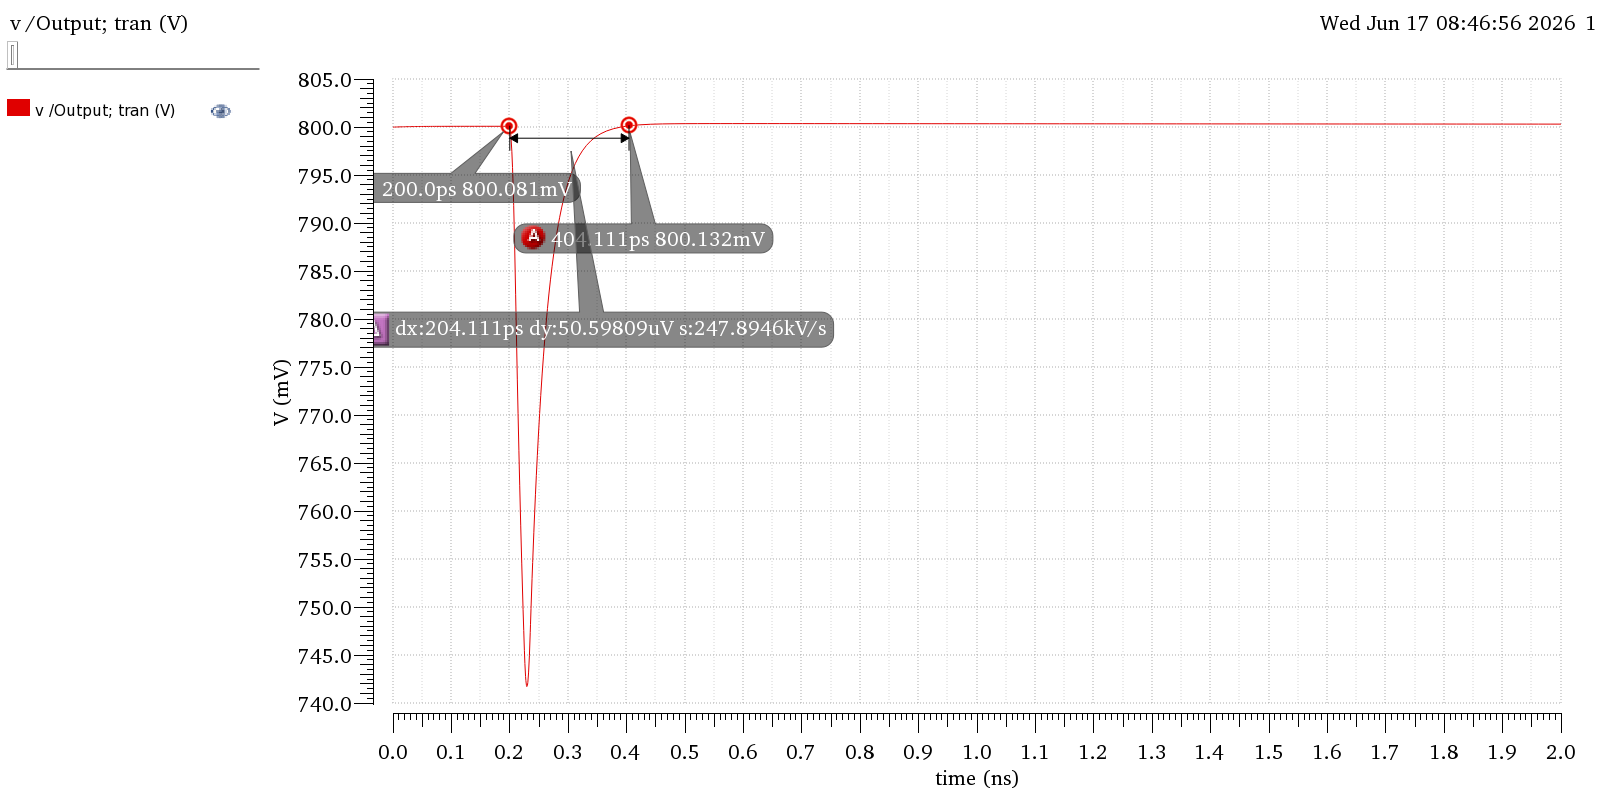
\includegraphics[width=0.85\textwidth]{chapter5/images/LDO/TS.png}
	\caption{Transient response of the reference buffer output to the
		same $30\,\text{mA}$ load step, with $C_{ref} = 0$.}
	\label{fig:vref_buffer_no_cref}
\end{figure}

With no decoupling capacitance at the output, $V_{out}$ momentarily
collapses by approximately $58\,\text{mV}$ immediately following the
load step, since the regulator loop alone must supply the entire
transient current demand. However, the feedback loop reacts quickly: the
two cursor measurements in Fig.~\ref{fig:vref_buffer_no_cref} show that
$V_{out}$ returns to within microvolts of $V_{ref}$ by
$t = 204.111\,\text{ps}$ after the disturbance begins. This recovery
time is well within the $277\,\text{ps}$ maximum settling time budget
allowed by the DAC's system-level timing requirement, leaving a margin of
approximately $73\,\text{ps}$ ($\approx 26\,\%$ of the allotted budget).

This result demonstrates that, even in the worst case of
$C_{ref} = 0$, the reference buffer's loop bandwidth
(Section~\ref{sec:vref_buffer_loop_gain}) is high enough to recover from
a full-scale load transient within the system's required settling
window. In practice, $C_{ref}$ is still included to further suppress the
\emph{magnitude} of the bounce itself, as derived analytically in
Section~\ref{sec:vref_bounce}, but this result confirms that the
buffer's closed-loop speed alone provides sufficient timing margin even
under the most pessimistic loading condition.

\subsection{TSPC Cell: Design and Simulation}

After the explanation of the TSPC cell in Section~\ref{sar}, the cell was designed to
achieve minimum propagation delay while producing a clean output free of glitches and
well-bounded between ground and $V_{DD}$.

\begin{figure}[h!]
	\centering
	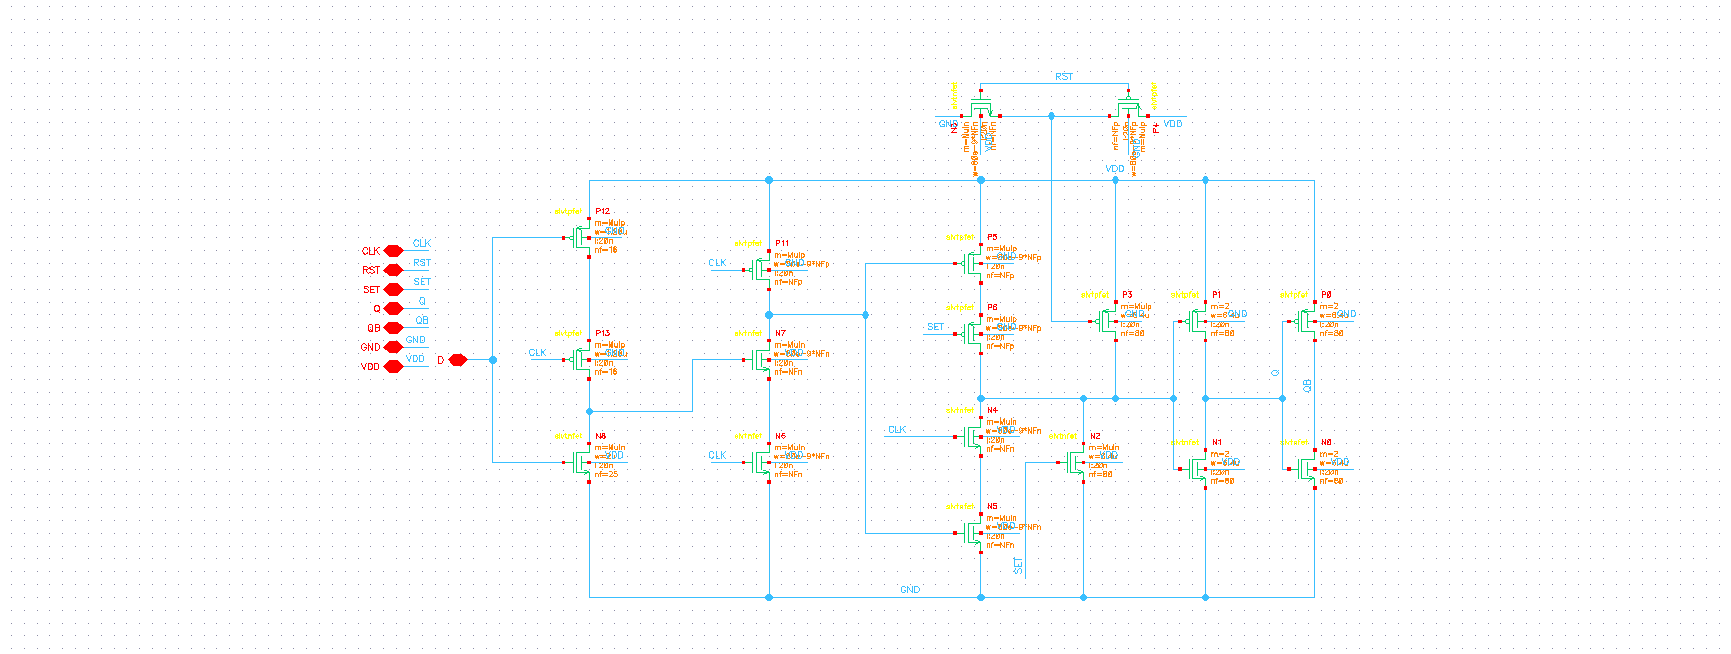
\includegraphics[width=1\textwidth]{chapter5/images/10.png}
	\caption{Schematic of the implemented TSPC cell}
	\label{fig:tspc_schematic_impl}
\end{figure}

Table~\ref{tab:tspc_devices} lists the transistor sizing used in the TSPC cell. All devices
are super low-$V_T$ (SLVT) to maximise switching speed at the target supply voltage.

\begin{table}[h!]
	\centering
	\caption{TSPC cell device parameters}
	\label{tab:tspc_devices}
	\renewcommand{\arraystretch}{1.3}
	\begin{tabular}{llllc}
		\toprule
		\textbf{Device} & \textbf{Type}   & \textbf{W}                  & \textbf{L} & \textbf{Mul} \\
		\midrule
		Mp12 & SLVTPFET & \SI{5}{\micro m}   & 20\,nm & 1 \\
		Mp13 & SLVTPFET & \SI{5}{\micro m}   & 20\,nm & 1 \\
		Mn8  & SLVTNFET & \SI{3.2}{\micro m} & 20\,nm & 1 \\
		Mn6  & SLVTNFET & \SI{6.4}{\micro m} & 20\,nm & 1 \\
		Mn7  & SLVTNFET & \SI{6.4}{\micro m} & 20\,nm & 1 \\
		Mp11 & SLVTPFET & \SI{10}{\micro m}  & 20\,nm & 1 \\
		Mp5  & SLVTPFET & \SI{8}{\micro m}   & 20\,nm & 1 \\
		Mp6  & SLVTPFET & \SI{8}{\micro m}   & 20\,nm & 1 \\
		Mn4  & SLVTNFET & \SI{6.4}{\micro m} & 20\,nm & 1 \\
		Mn5  & SLVTNFET & \SI{6.4}{\micro m} & 20\,nm & 1 \\
		Mp4  & SLVTNFET & \SI{8}{\micro m}   & 20\,nm & 1 \\
		Mp3  & SLVTPFET & \SI{6.4}{\micro m} & 20\,nm & 1 \\
		Mn2  & SLVTNFET & \SI{6.4}{\micro m} & 20\,nm & 1 \\
		Mp12 & SLVTNFET & \SI{6.4}{\micro m} & 20\,nm & 1 \\
		Mn1  & SLVTNFET & \SI{6.4}{\micro m} & 20\,nm & 2 \\
		Mn0  & SLVTNFET & \SI{6.4}{\micro m} & 20\,nm & 2 \\
		Mp1  & SLVTPFET & \SI{6.4}{\micro m} & 20\,nm & 2 \\
		Mp0  & SLVTPFET & \SI{6.4}{\micro m} & 20\,nm & 2 \\
		\bottomrule
	\end{tabular}
\end{table}

The primary metrics used to evaluate the TSPC cell are propagation delay and correct
functional operation of the Set, Reset, and data-capture (buffer) modes.

\begin{figure}[h!]
	\centering
	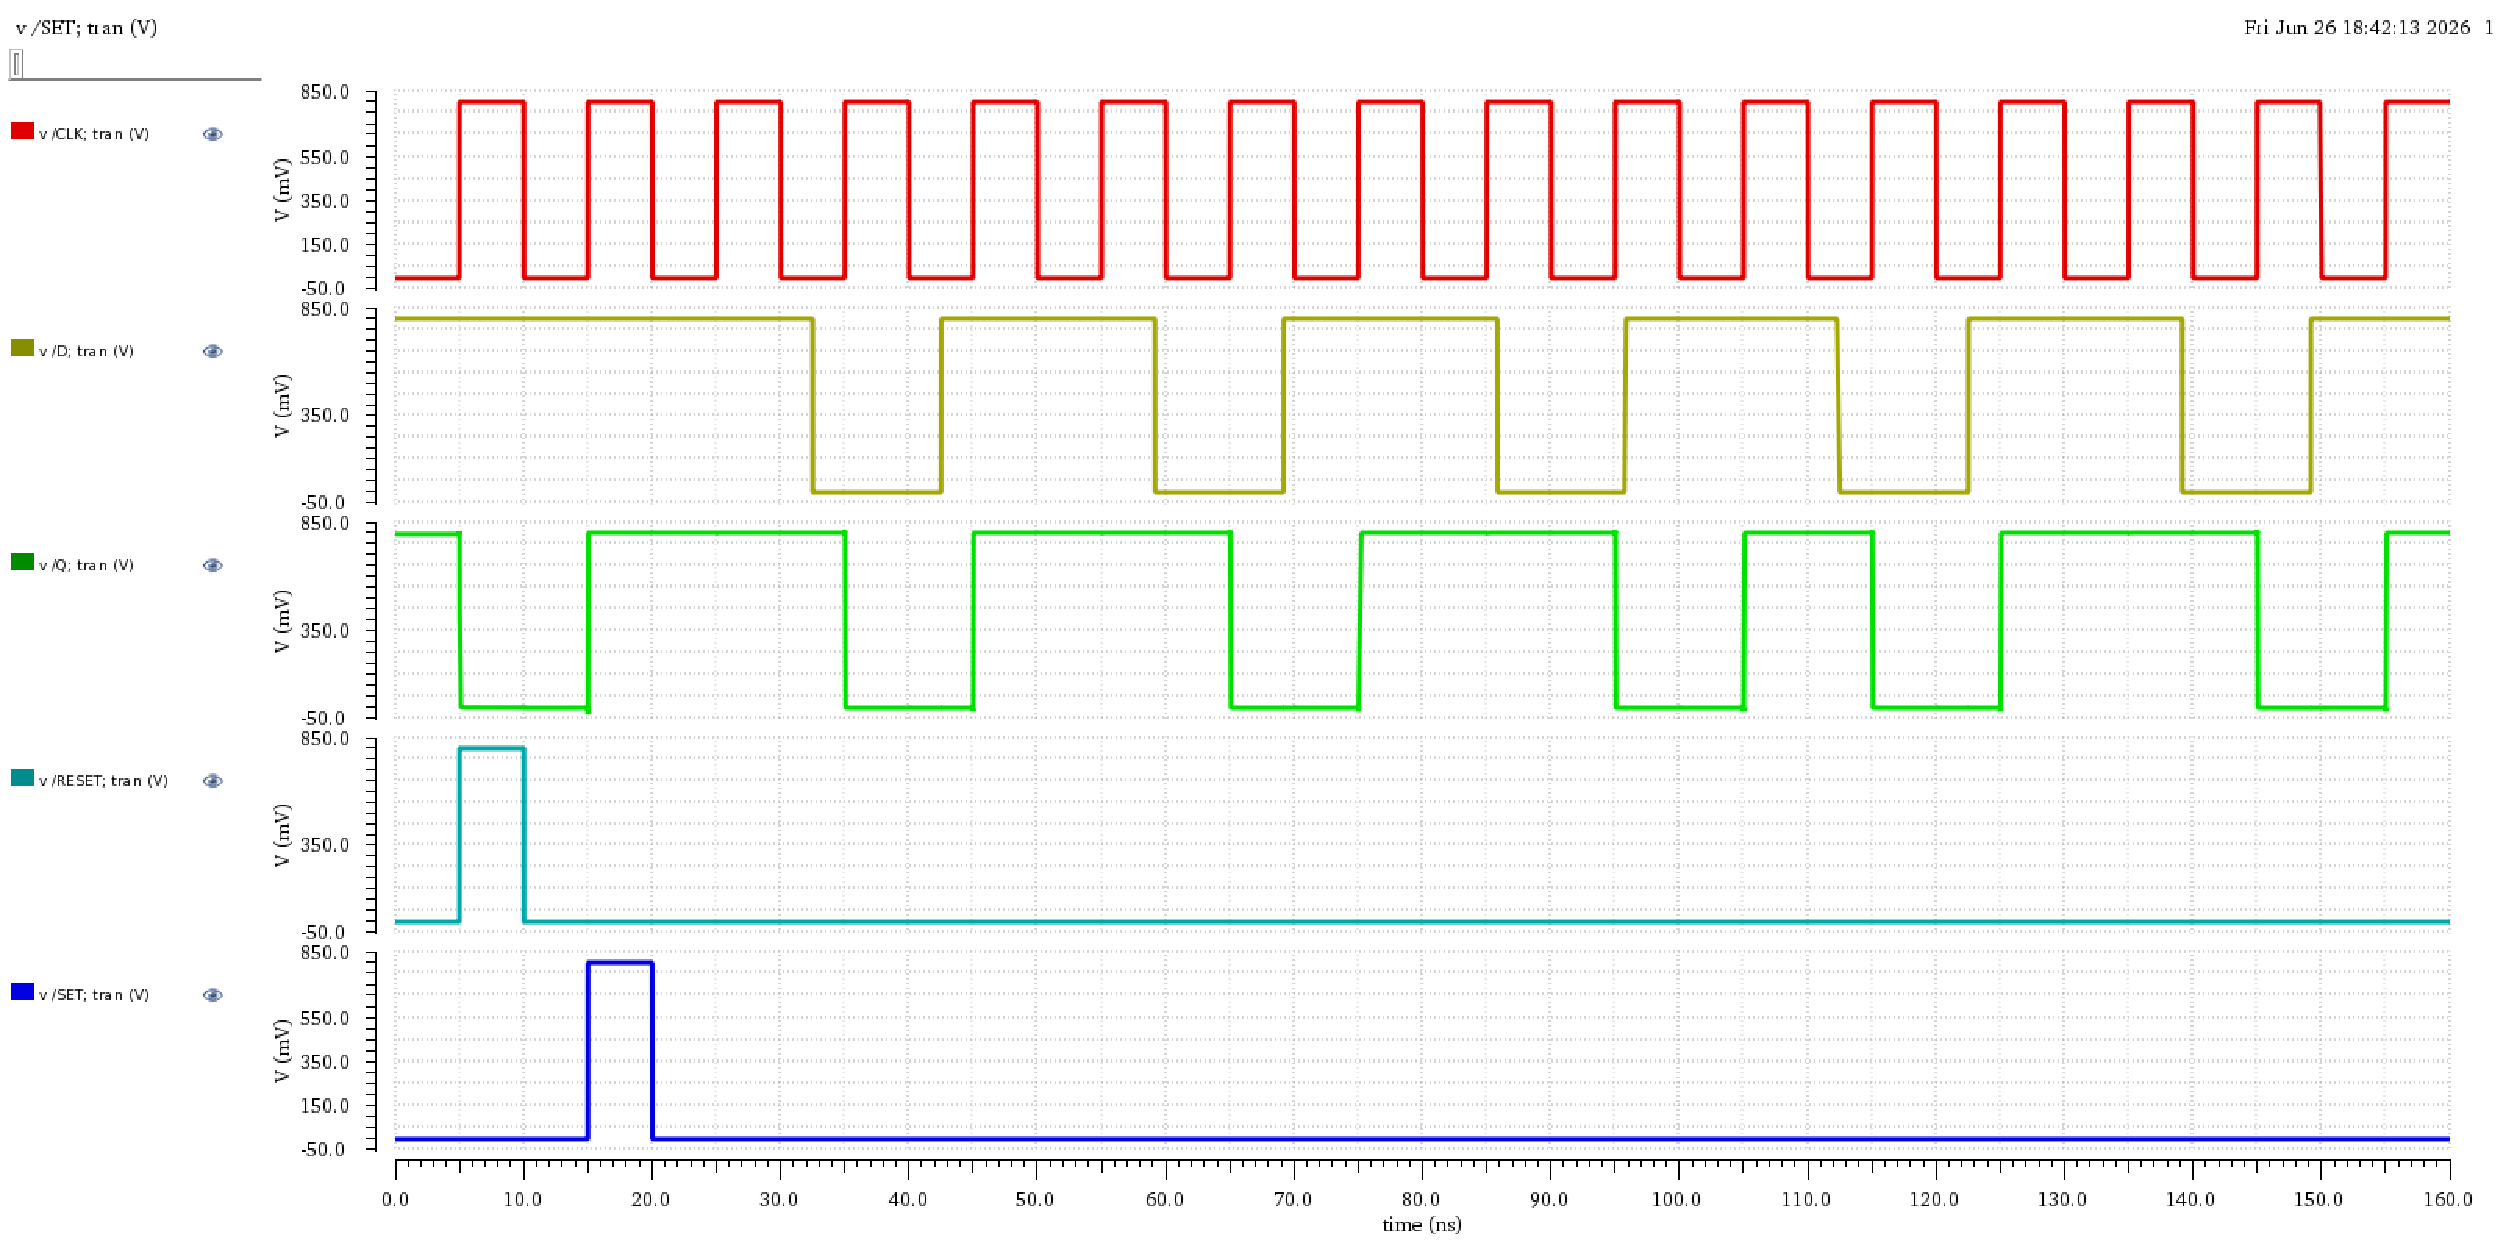
\includegraphics[width=0.8\textwidth]{chapter5/images/11.pdf}
	\caption{TSPC cell input, output, and control signals}
	\label{fig:tspc_waveforms}
\end{figure}

As shown in Fig.~\ref{fig:tspc_waveforms}, when Reset is asserted, the output $Q$ is pulled
to ground. Once Set is subsequently asserted, $Q$ returns to $V_{DD}$. With both asynchronous
overrides deasserted and the clock high, $Q$ correctly tracks the input $D$ for both
low-to-high and high-to-low transitions, confirming correct functional operation.

\begin{figure}[h!]
	\centering
	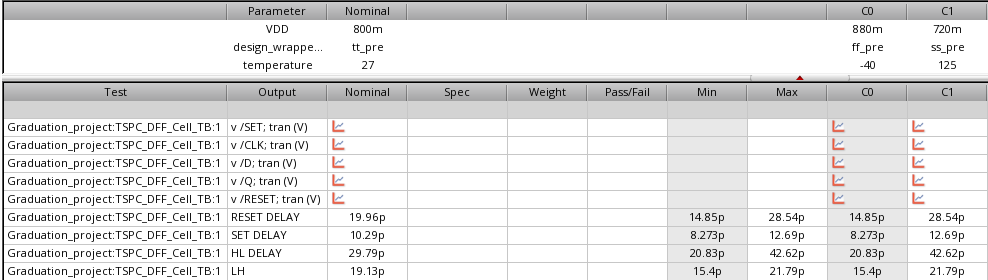
\includegraphics[width=0.8\textwidth]{chapter5/images/12.png}
	\caption{TSPC cell propagation delay across process corners}
	\label{fig:tspc_corners}
\end{figure}

Table~\ref{tab:tspc_delay} summarises the measured propagation delay for each operation mode
across the Typical (TT), Fast--Fast (FF), and Slow--Slow (SS) process corners.

\begin{table}[h!]
	\centering
	\caption{TSPC cell propagation delay across process corners}
	\label{tab:tspc_delay}
	\renewcommand{\arraystretch}{1.3}
	\begin{tabular}{lccc}
		\toprule
		\textbf{Operation} &
		\textbf{TT, \SI{27}{\celsius}} &
		\textbf{FF, \SI{125}{\celsius}, $-10\%\,V_{DD}$} &
		\textbf{SS, \SI{-40}{\celsius}, $+10\%\,V_{DD}$} \\
		\midrule
		Set          & \SI{10.3}{ps} & \SI{12.7}{ps} & \SI{8.27}{ps} \\
		Reset        & \SI{20.0}{ps} & \SI{28.5}{ps} & \SI{14.85}{ps} \\
		High-to-low  & \SI{29.8}{ps} & \SI{42.6}{ps} & \SI{20.8}{ps} \\
		Low-to-high  & \SI{19.0}{ps} & \SI{21.8}{ps} & \SI{15.4}{ps} \\
		\bottomrule
	\end{tabular}
\end{table}

The worst-case delay occurs in the high-to-low transition, as this path traverses a greater
number of internal nodes compared to the low-to-high path. The Set and Reset operations
exhibit lower delays because their control signals are connected directly to the stage
preceding the output inverter, bypassing the longer internal data path.

\subsection{Ring Counter and Data Register Simulation}

Following the verification of the individual TSPC cell, 12 DFFs were connected to construct
the ring counter and 11 DFFs to construct the data register, forming the complete SAR logic
block.

\begin{figure}[h!]
	\centering
	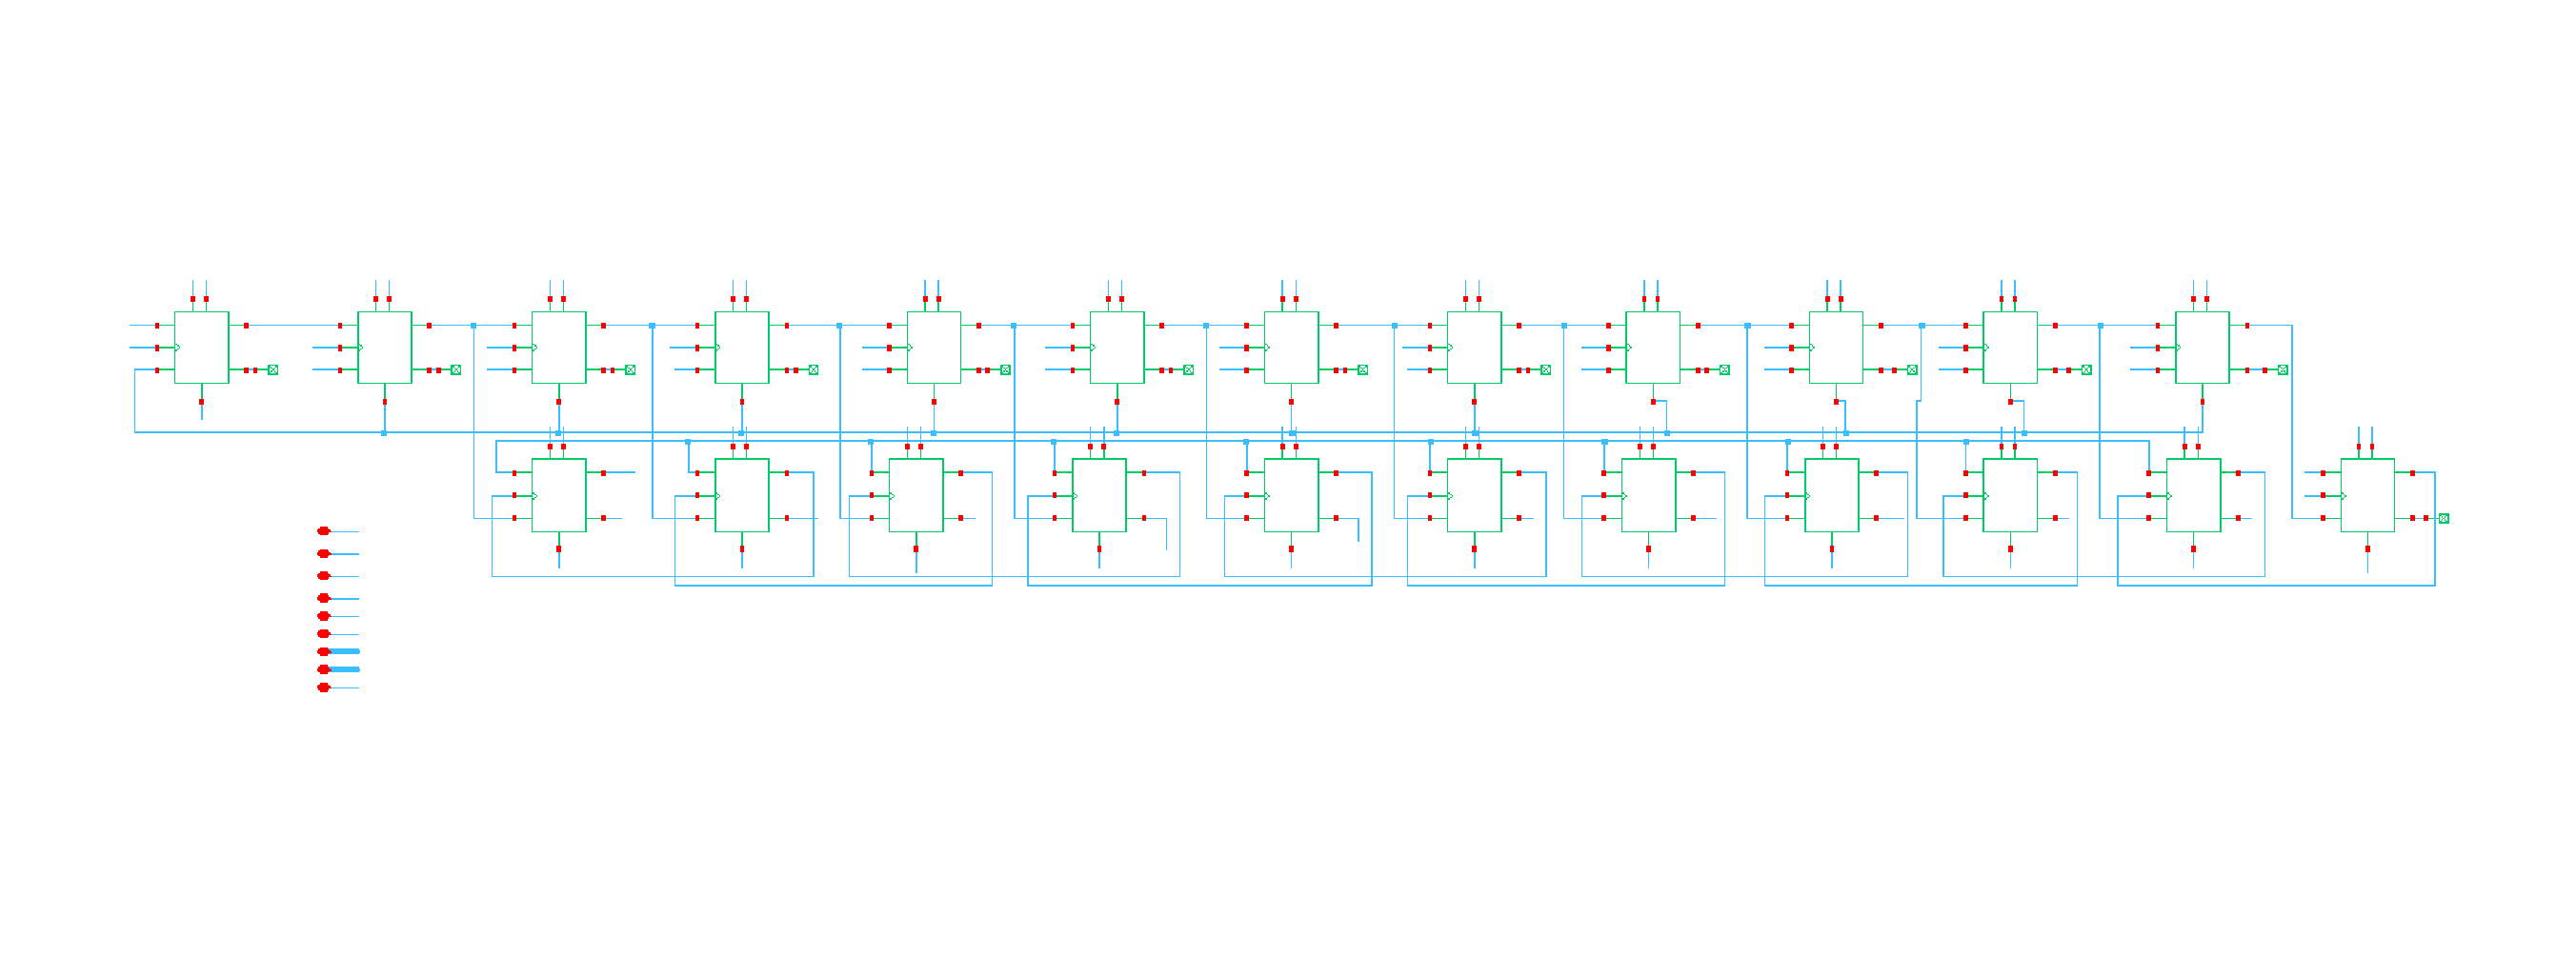
\includegraphics[width=0.9\textwidth]{chapter5/images/13.pdf}
	\caption{Schematic of the SAR logic block}
	\label{fig:sar_logic_schematic}
\end{figure}

To verify the correct operation of the SAR logic within the ADC environment, three
representative test cases were simulated, corresponding to a comparator output that is
permanently low, permanently high, and alternating between both states.

\begin{figure}[h!]
	\centering
	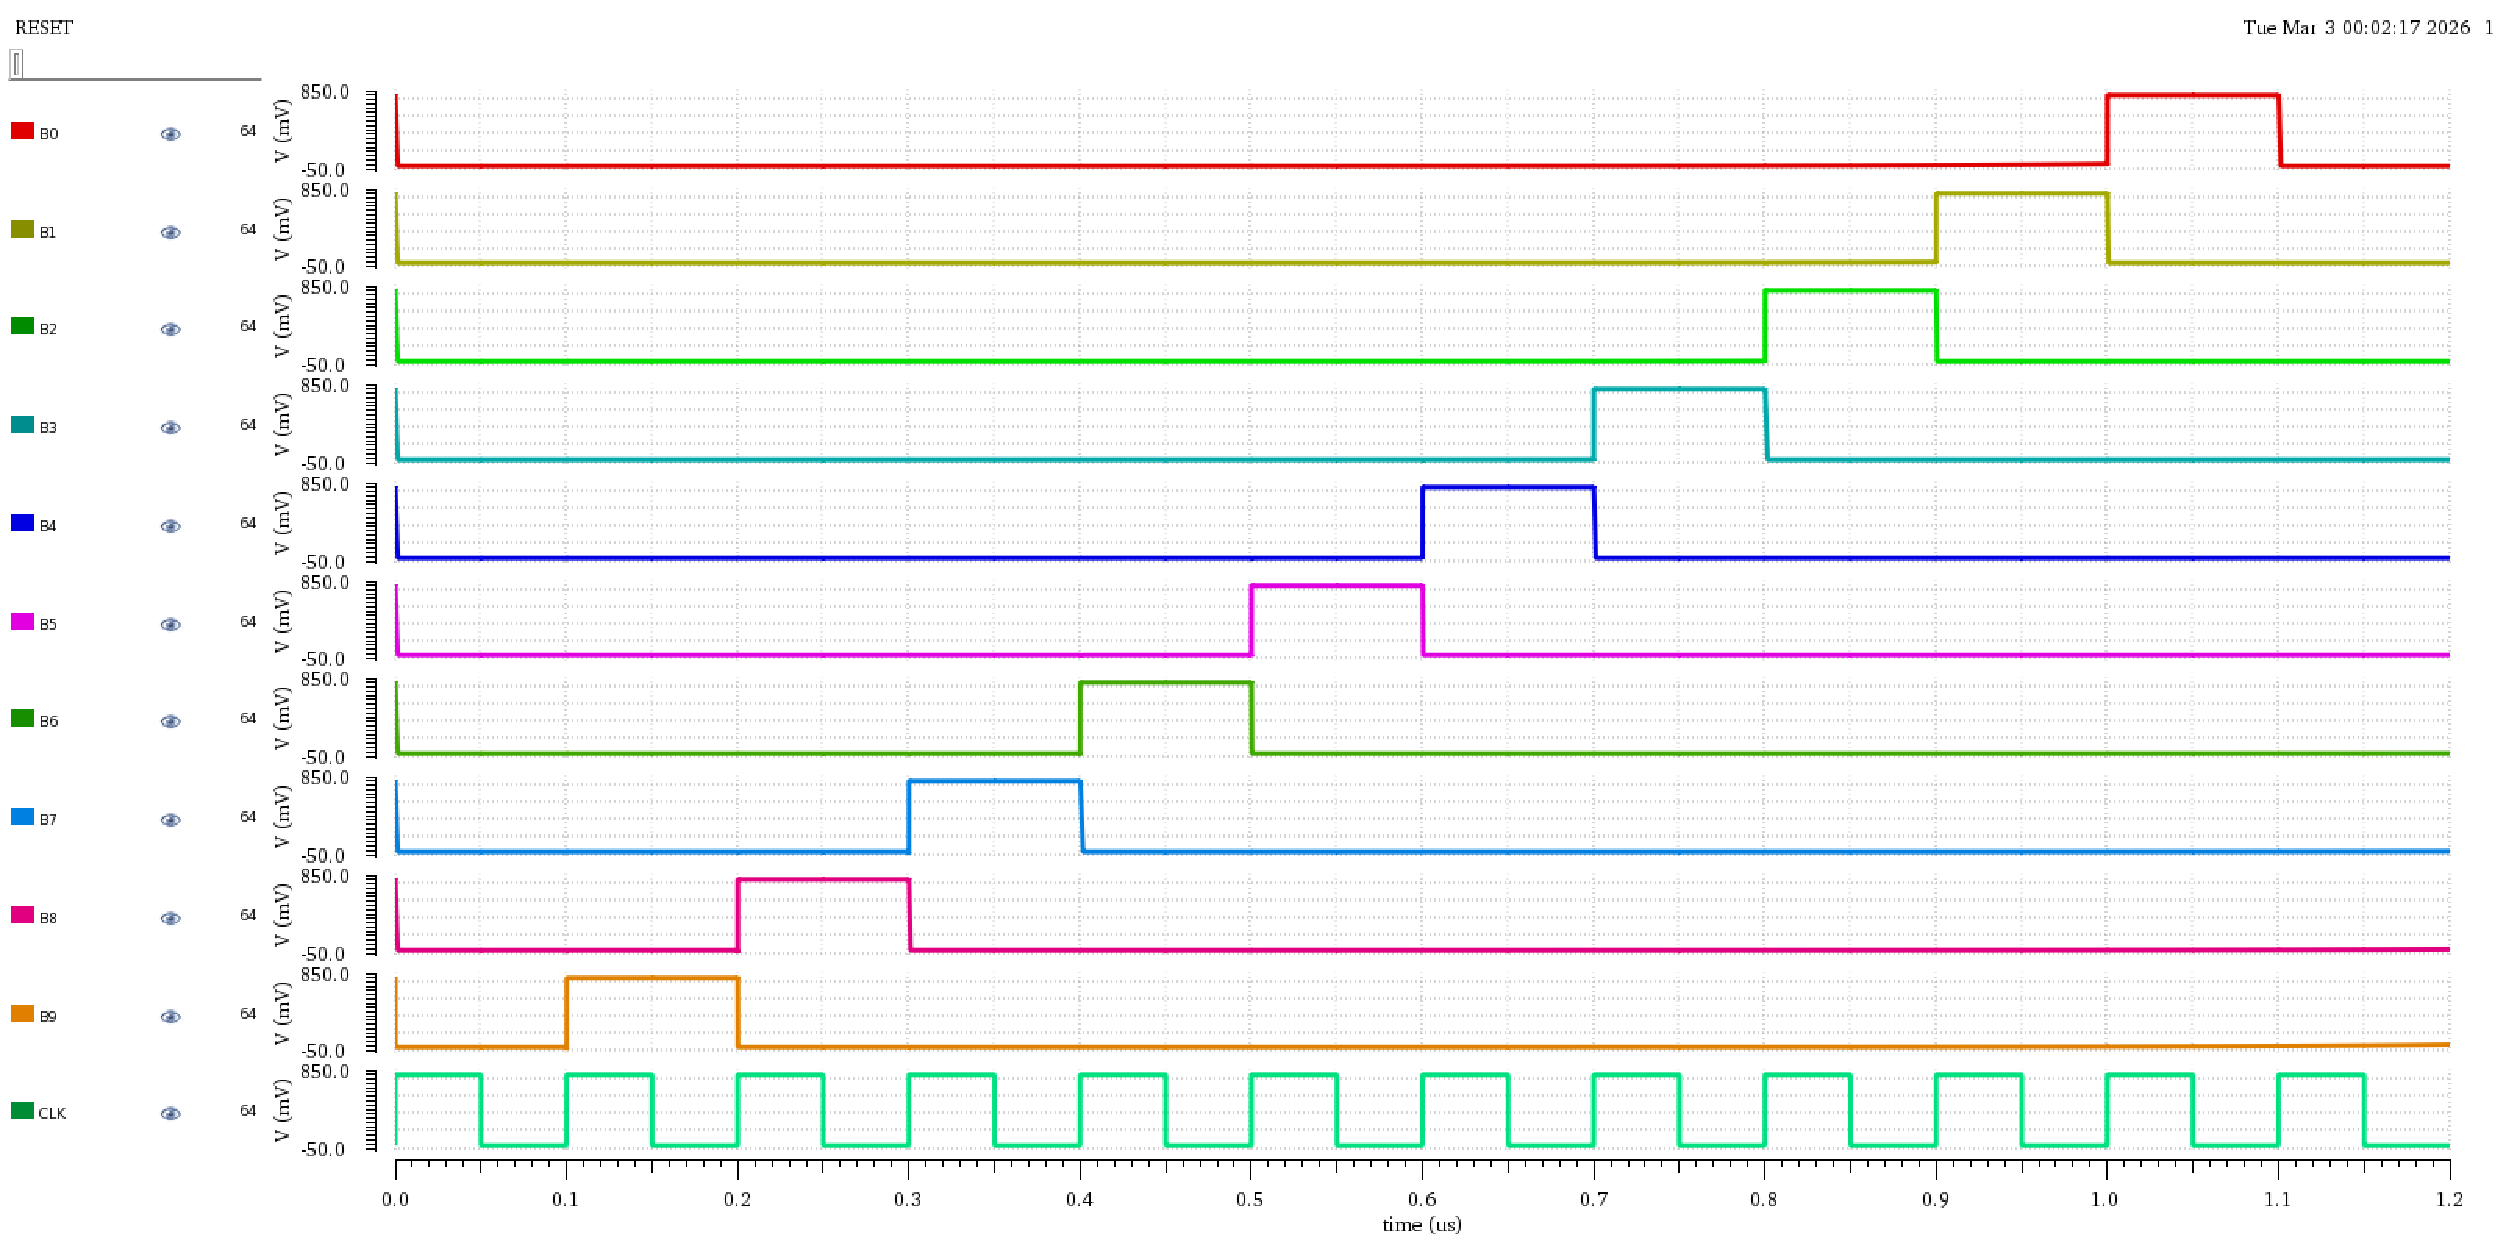
\includegraphics[width=0.8\textwidth]{chapter5/images/14.pdf}
	\caption{SAR logic output waveforms with comparator output held low}
	\label{fig:sar_out_low}
\end{figure}

\begin{figure}[h!]
	\centering
	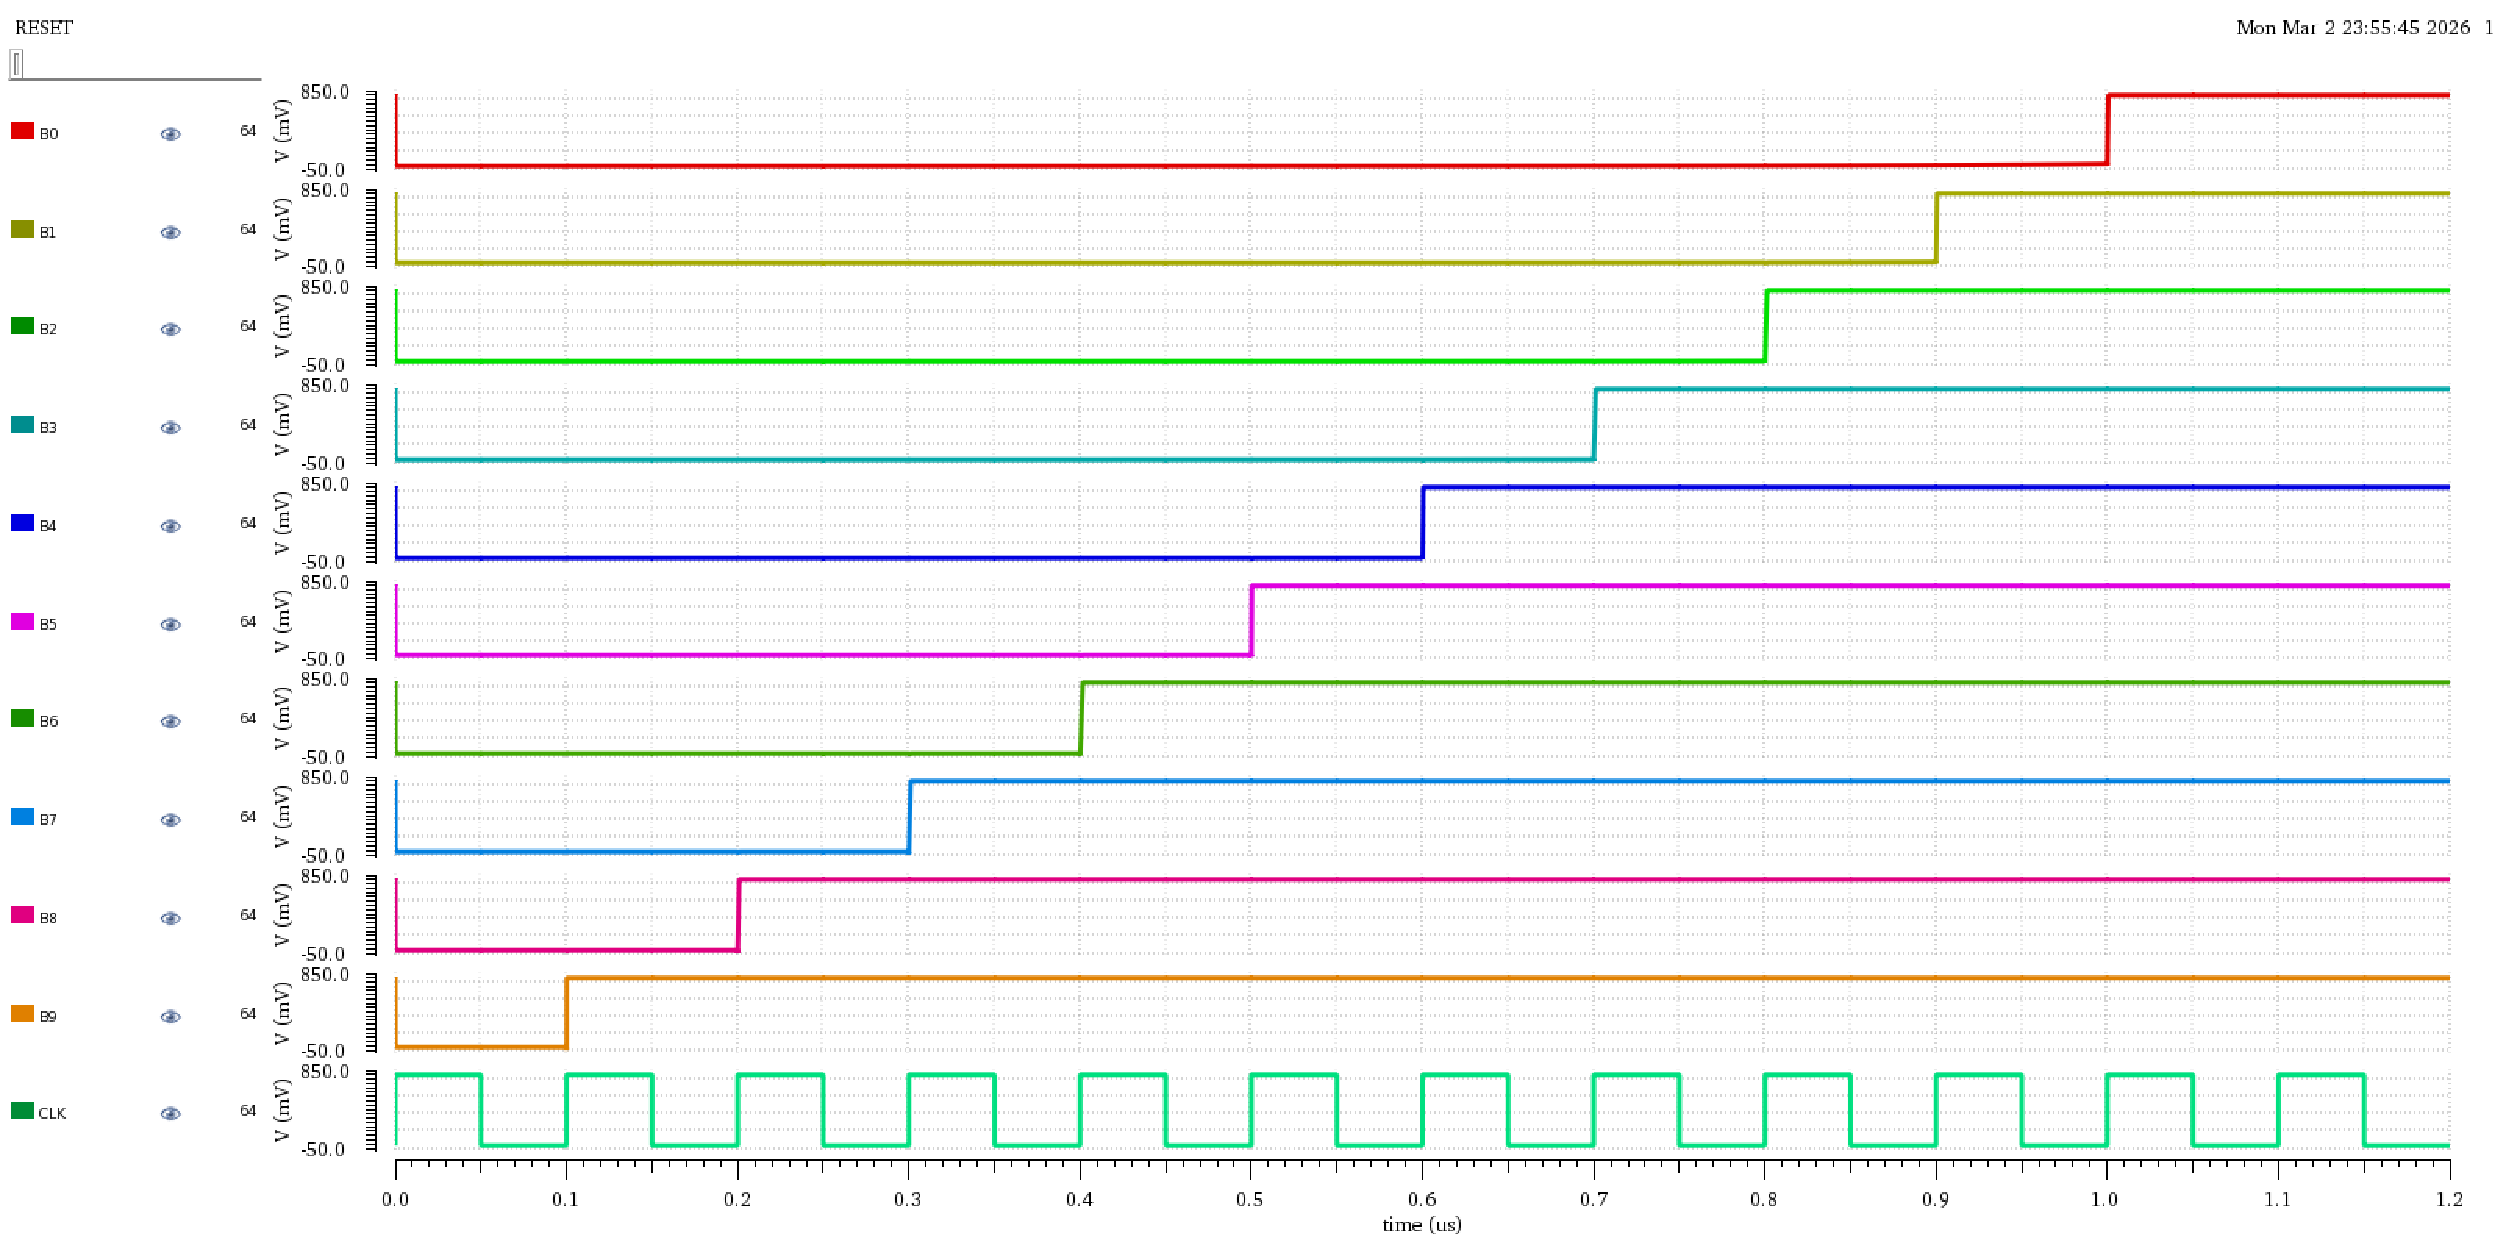
\includegraphics[width=0.8\textwidth]{chapter5/images/15.pdf}
	\caption{SAR logic output waveforms with comparator output held high}
	\label{fig:sar_out_high}
\end{figure}

\begin{figure}[h!]
	\centering
	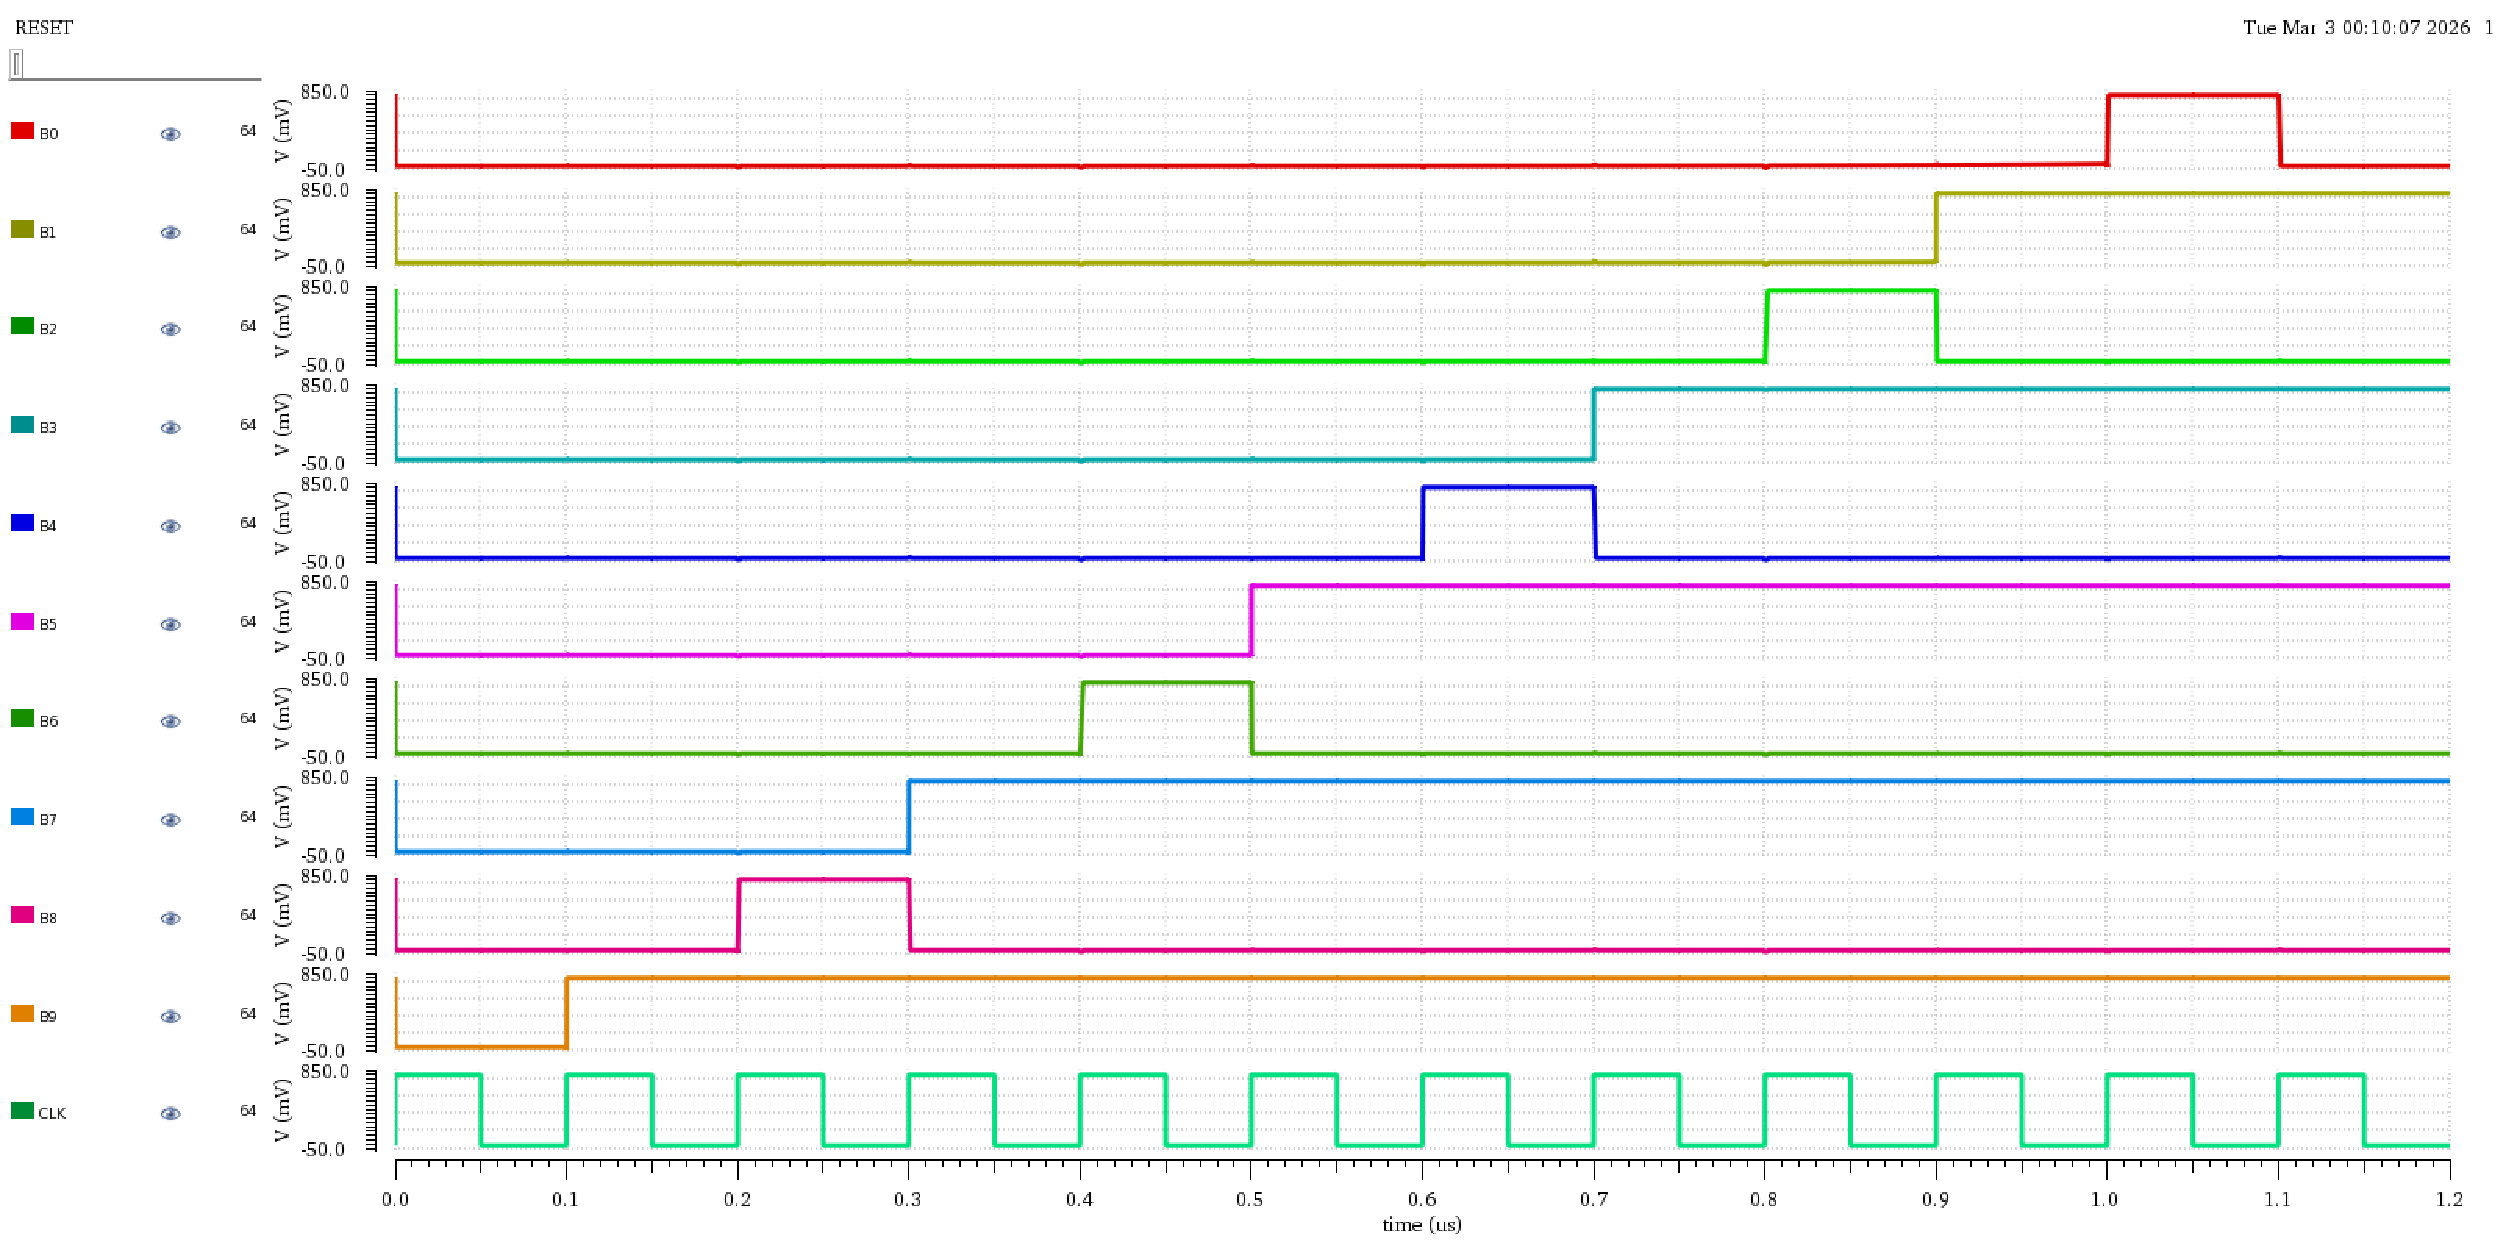
\includegraphics[width=0.8\textwidth]{chapter5/images/16.pdf}
	\caption{SAR logic output waveforms with alternating comparator output}
	\label{fig:sar_out_alternating}
\end{figure}

The simulation results across all three cases confirm correct and reliable operation of the
SAR logic. The ring counter token propagates sequentially through all stages, and the data
register accurately latches the comparator decision at each conversion step. The block is
therefore ready for integration into the complete SAR ADC slice.

\section{SAR ADC Slice Integration}
% ══════════════════════════════════════════════════════════════════════════════

Following the individual design and verification of each sub-block, all components were
integrated to form the complete SAR ADC slice. The integration was initially performed using
ideal component models to validate the system-level operation, after which each ideal element
was progressively replaced with its actual circuit implementation.

\begin{figure}[h!]
	\centering
	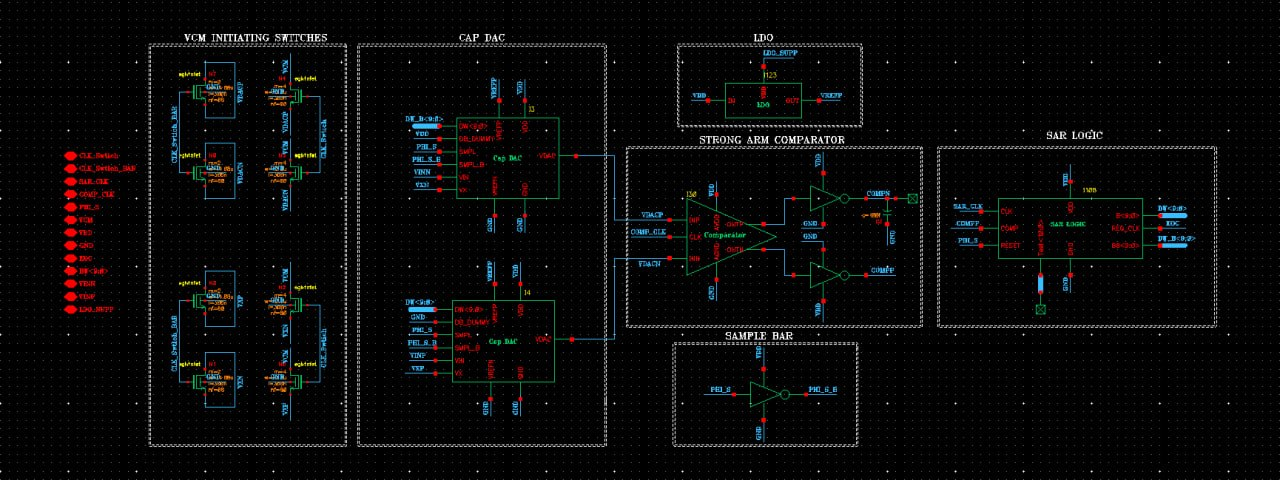
\includegraphics[width=0.95\textwidth]{chapter5/images/17j.jpg}
	\caption{Top-level schematic of the SAR ADC slice}
	\label{fig:sar_slice}
\end{figure}

As illustrated in Fig.~\ref{fig:sar_slice}, several additional components are present beyond
the core blocks: output inverters after the comparator, $V_{CM}$-initiating switches, and a
load capacitor at the comparator output.

\paragraph{Comparator output inverters.}
These inverters serve two purposes. First, they buffer and clean the comparator output,
suppressing glitches before the signal reaches the SAR logic. Second, during the comparator
reset phase the output must be driven low, since the SAR logic clock is high at that time;
presenting a high level to the data register inputs would corrupt the ongoing conversion.
The inverter chain ensures the output defaults to a logic low during reset.

\paragraph{Load capacitor.}
The data register consists of 11 DFFs, and each DFF's data input ($D$) is connected to two
transistors whose combined parasitic capacitance is approximately \SI{8}{fF} per cell,
yielding a total load of roughly \SI{88}{fF} on the comparator output node. A matching load
capacitor is placed on the complementary output node to balance both sides of the differential
pair, preventing a node-race condition that could corrupt the bit decision.

\paragraph{$V_{CM}$-initiating switches.}
These switches pre-charge the CDAC output nodes to $V_{DD}/2$ prior to each conversion cycle,
establishing a common-mode voltage of $V_{DD}/2$ at the comparator inputs. This is critical
for two reasons: it ensures the comparator input devices are biased in their active region at
the start of conversion, and it guarantees that the CDAC output remains bounded between
\SI{0}{V} and $V_{DD}$ throughout the binary search. The CDAC output voltage is given by

\begin{equation}
	V_{\mathrm{DAC}} = V_{CM} + V_{DD} \cdot \frac{C_{\mathrm{on}}}{C_{\mathrm{off}}} - V_{\mathrm{in}}
\end{equation}

For the first conversion cycle this reduces to

\begin{equation}
	V_{\mathrm{DAC}} = V_{CM} + \frac{V_{DD}}{2} - V_{\mathrm{in}}
\end{equation}

If $V_{\mathrm{in}} = 0$ and $V_{CM} > V_{DD}/2$, then $V_{\mathrm{DAC}} > V_{DD}$, which
would exceed the voltage rating of the comparator input devices. Pre-charging to exactly
$V_{DD}/2$ prevents this condition.

The switch transistors use extended gate low-$V_T$ NFET (eglvtnfet) devices with a nominal
gate voltage of \SI{1.8}{V}, chosen for their well-characterised operating regime. Their sizes
are carefully selected to minimise leakage in the off state while maintaining a sufficiently
low on-resistance to settle within the sampling clock period. Two diode-connected devices
(drain tied to source) are placed in parallel with each switch to compensate the clock
feedthrough charge injected through the gate--drain parasitic capacitance of the sampling
switch when the clock falls; their gates are driven by the inverted sampling clock.

\begin{figure}[h!]
	\centering
	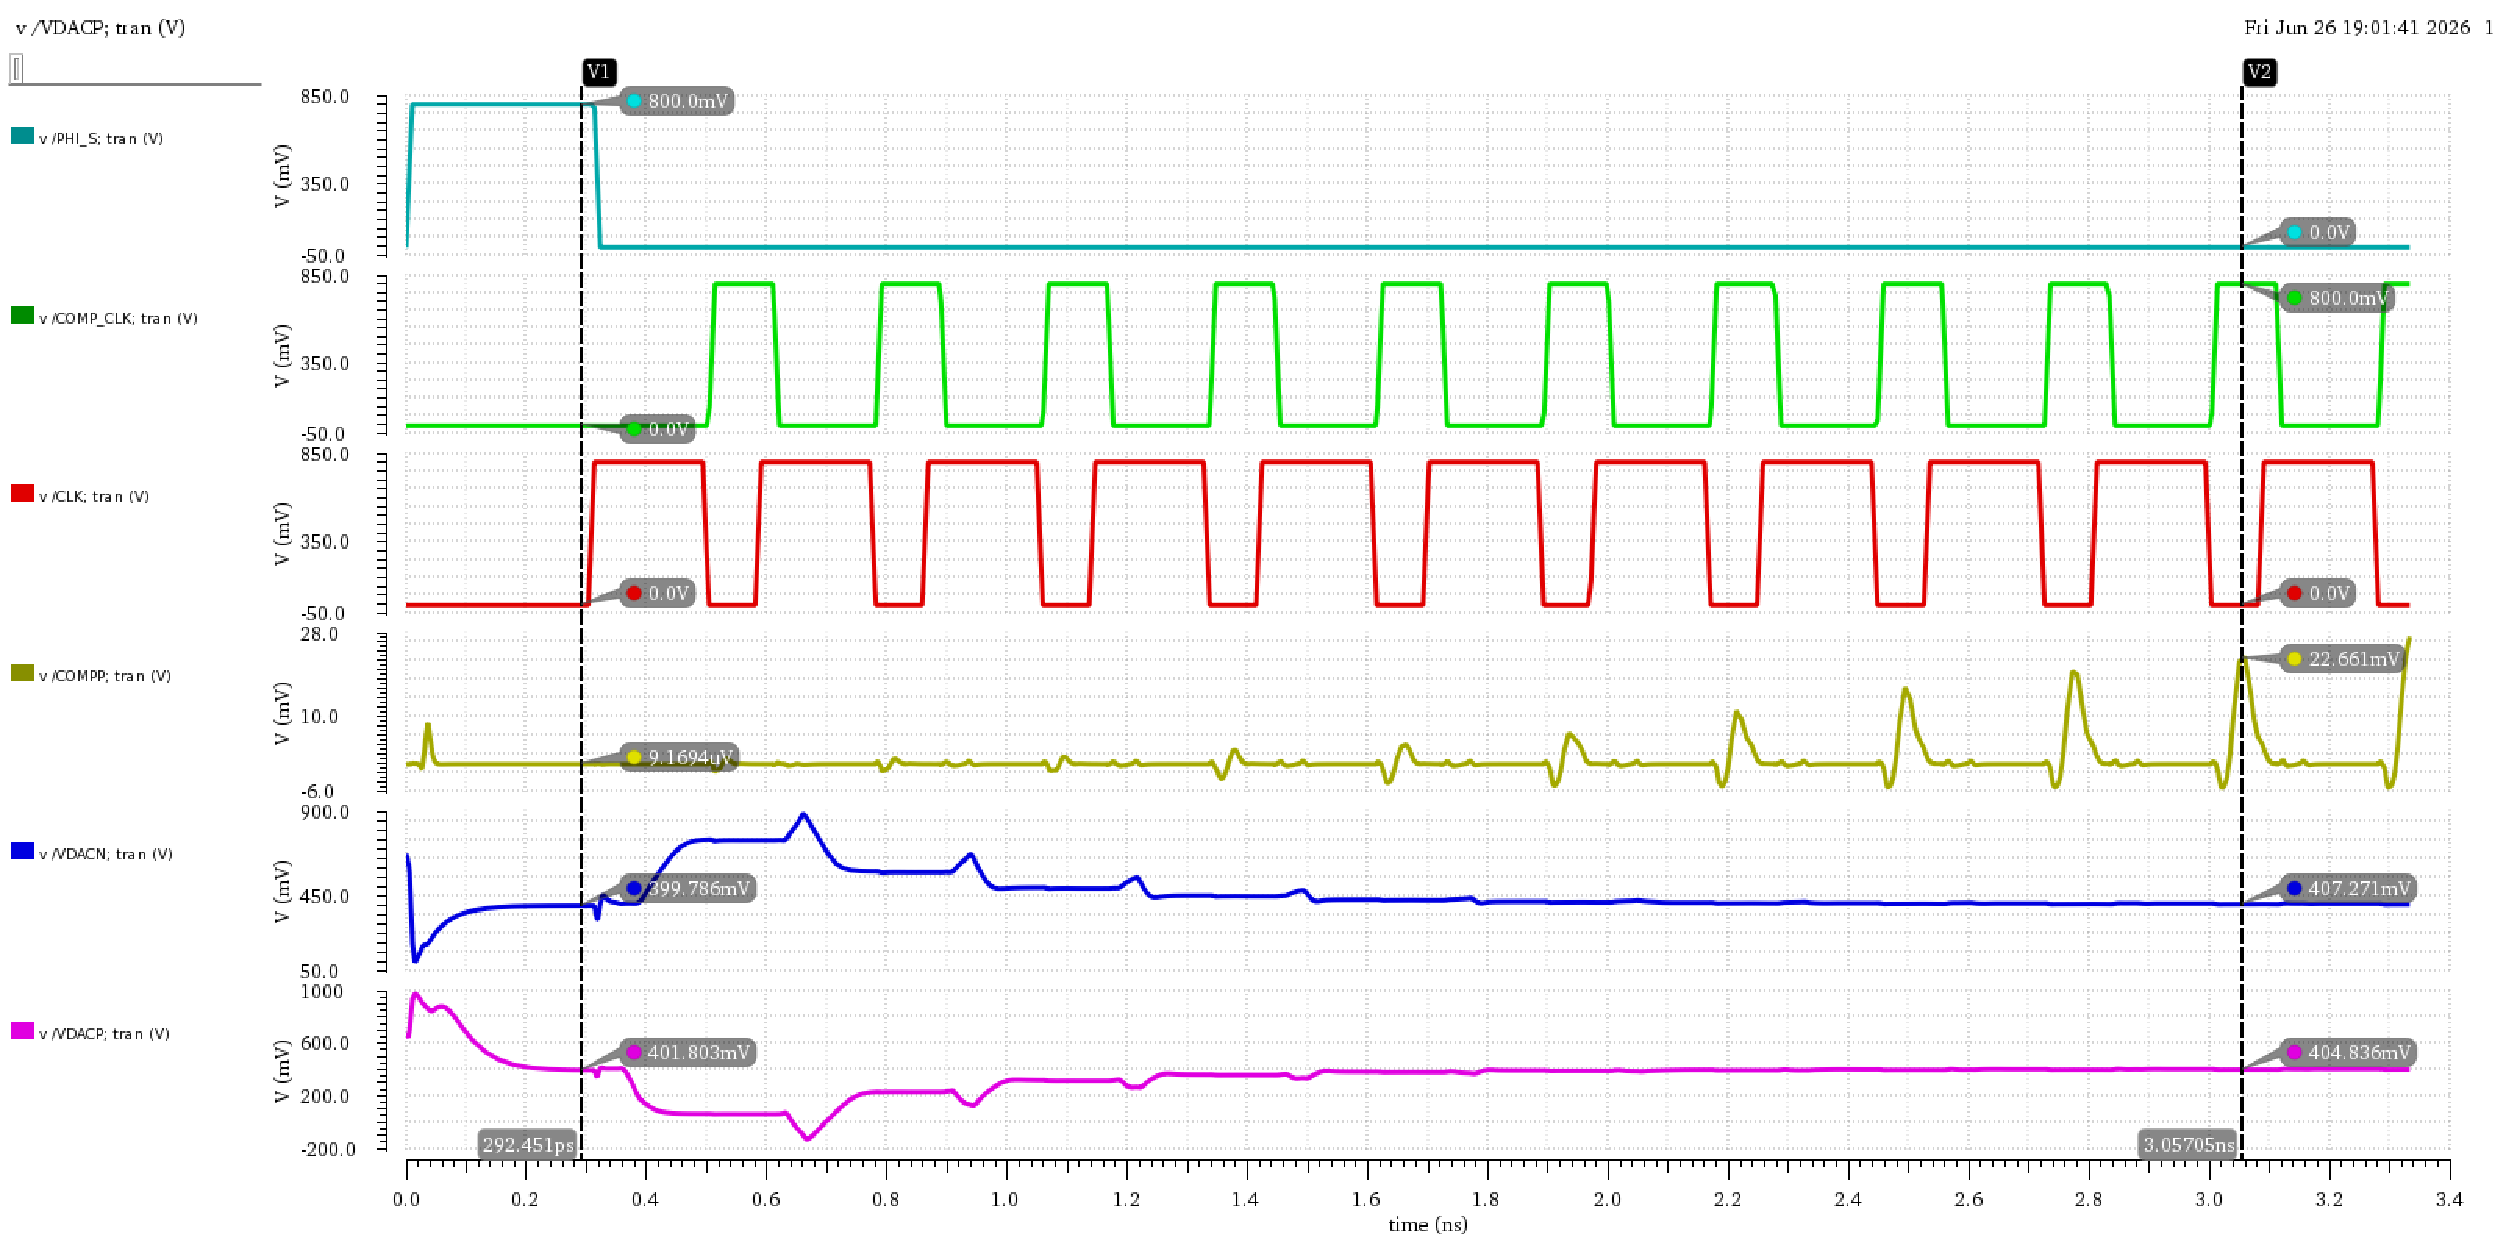
\includegraphics[width=0.8\textwidth]{chapter5/images/18.pdf}
	\caption{Control signal timing diagram for the SAR ADC slice}
	\label{fig:control_signals}
\end{figure}

Fig.~\ref{fig:control_signals} illustrates the timing relationship between the control
signals. The SAR logic clock activates as the sampling phase ends. After the MSB trial code
is applied to the bottom-plate switches and the CDAC output has settled, the comparator clock
rises to initiate the first comparison. A deliberate overlap between the comparator clock and
the SAR logic clock ensures that the data register DFFs capture the comparator decision before
the comparator resets and its output returns high.

% ══════════════════════════════════════════════════════════════════════════════
\subsection{DC Testing}
% ══════════════════════════════════════════════════════════════════════════════

Before dynamic tests, DC sweeps were performed to verify the static operation of the slice at
three representative input levels.

\begin{figure}[h!]
	\centering
	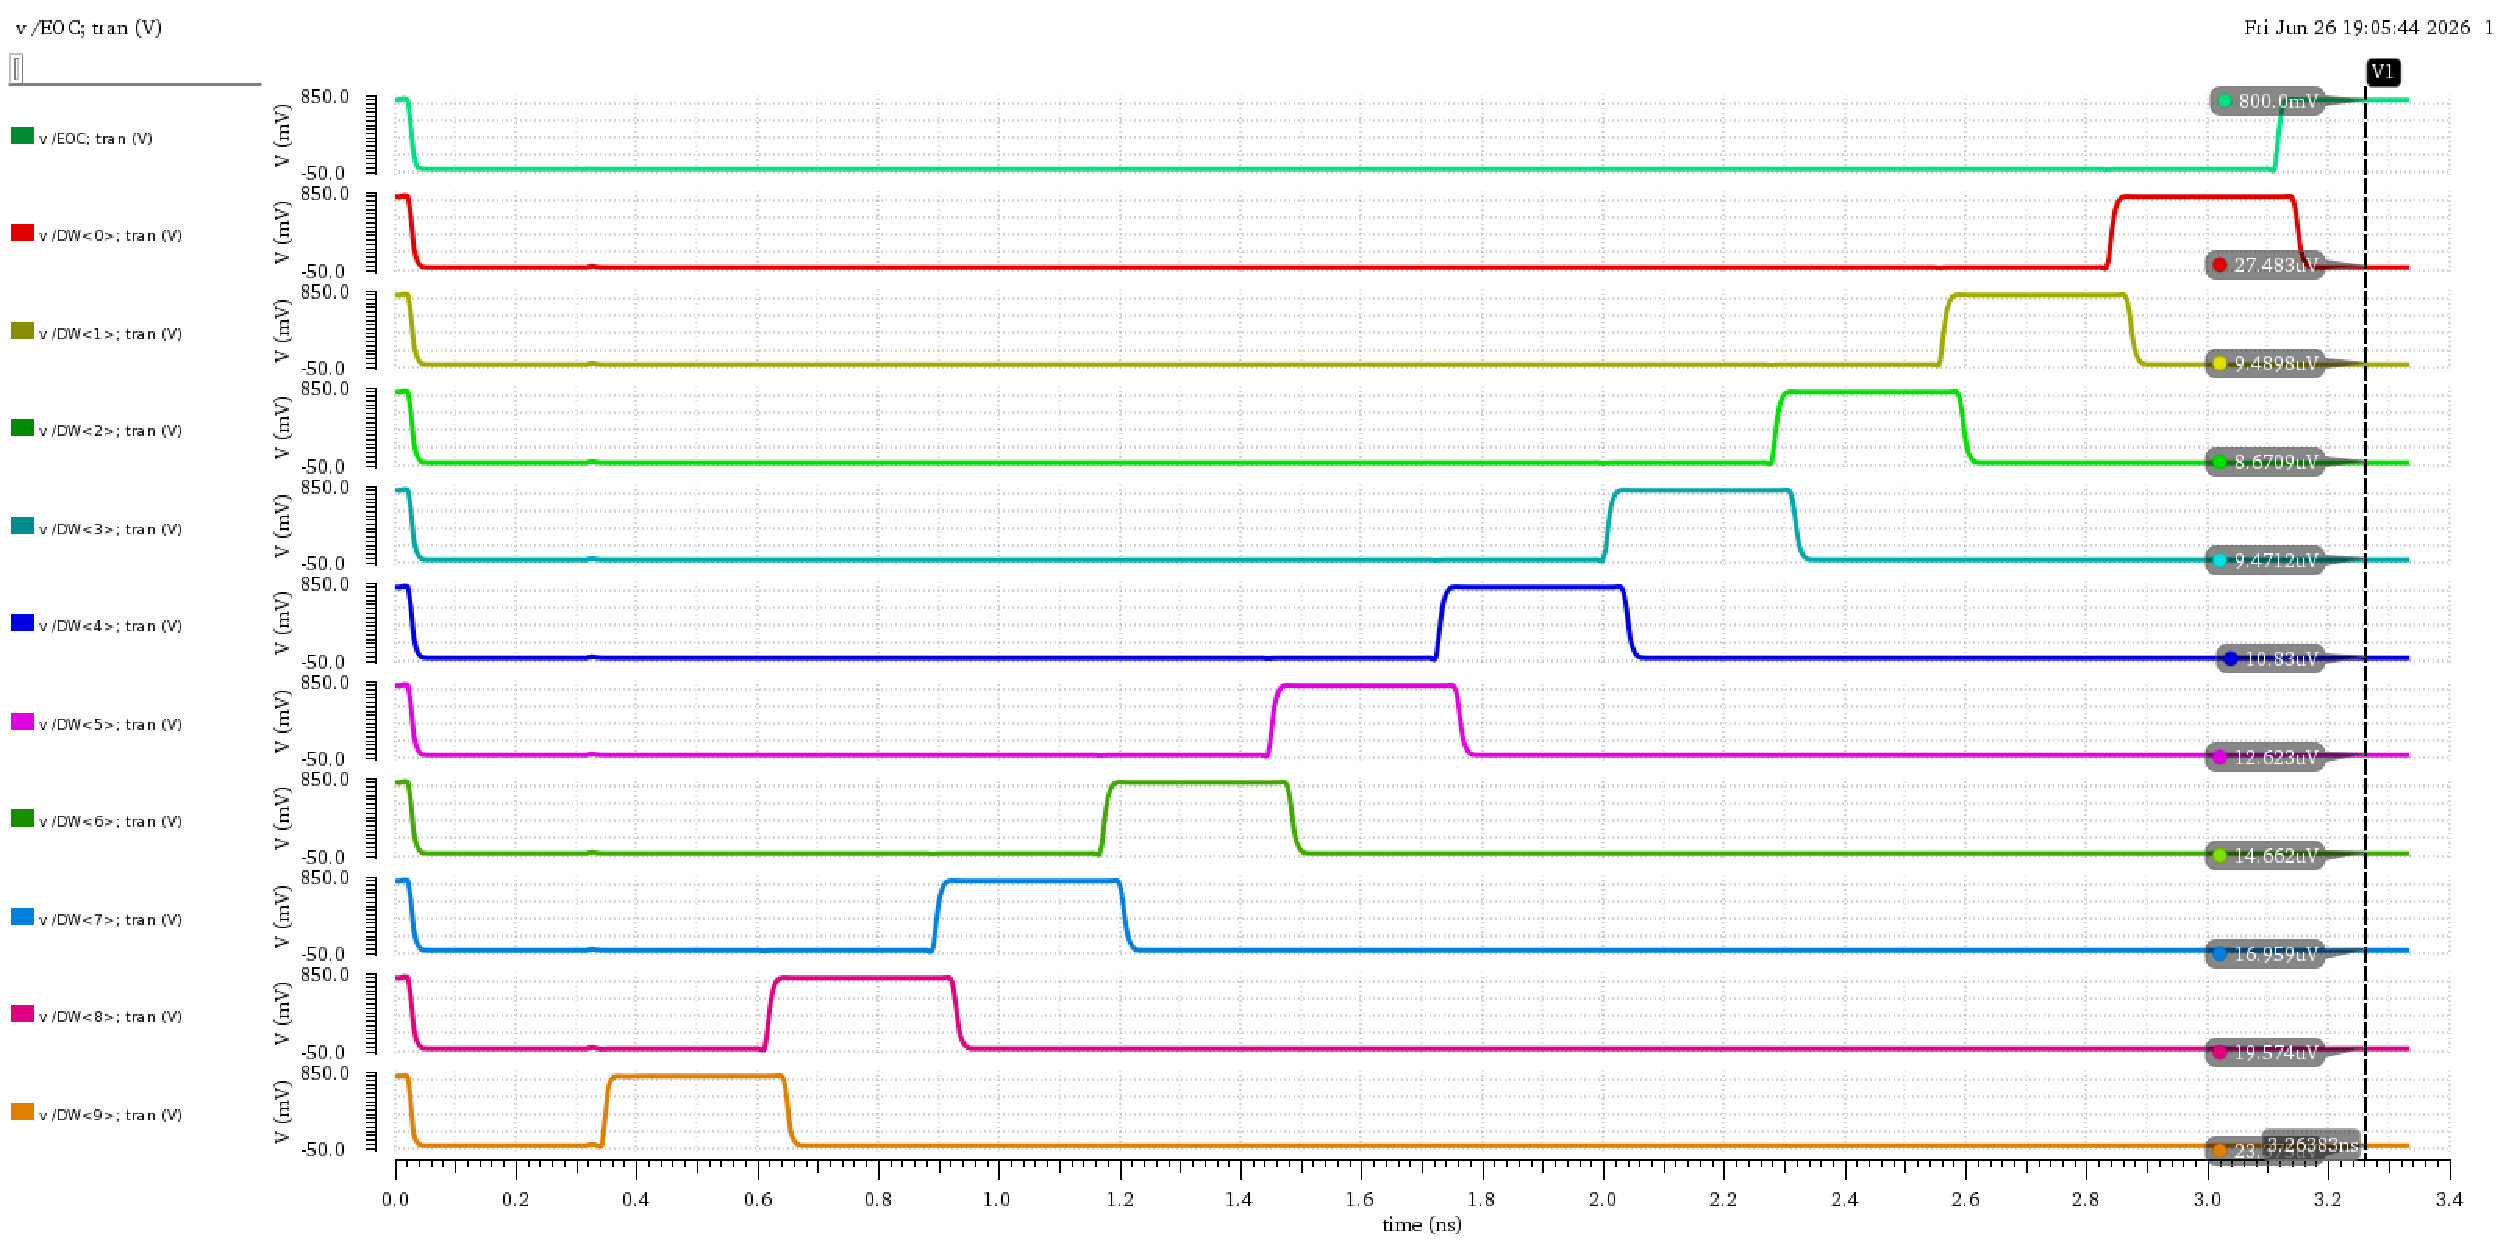
\includegraphics[width=0.75\textwidth]{chapter5/images/19.pdf}
	\caption{Digital output for $V_{\mathrm{in}} = \SI{-800}{mV}$}
	\label{fig:dc_neg800}
\end{figure}

\begin{figure}[h!]
	\centering
	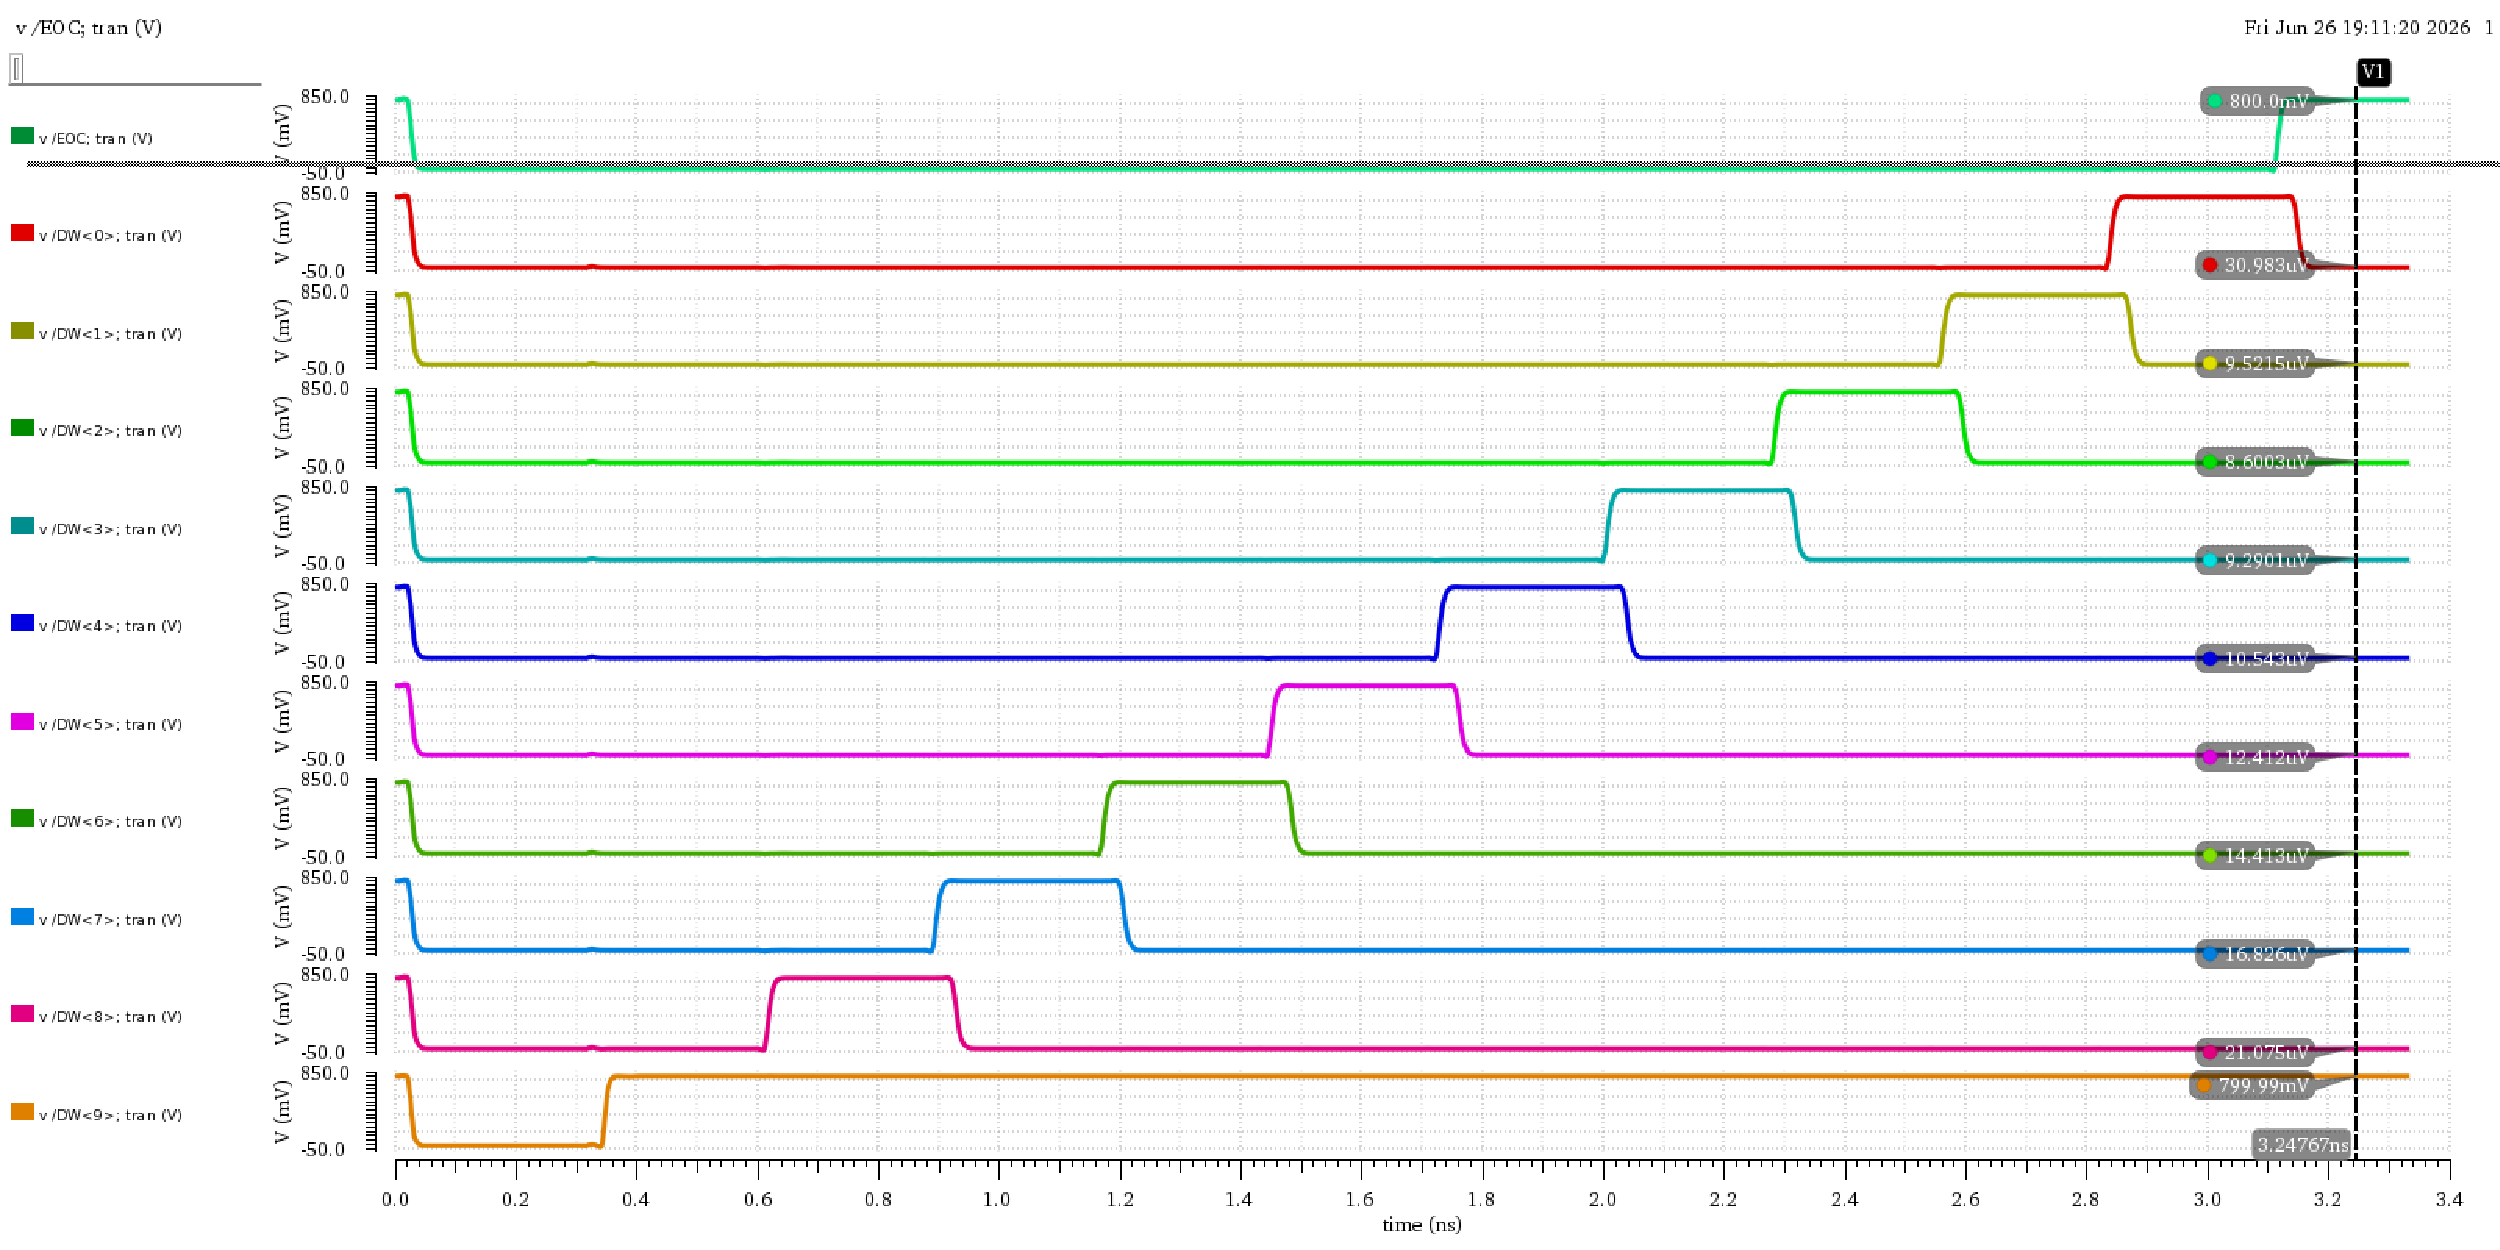
\includegraphics[width=0.75\textwidth]{chapter5/images/20.pdf}
	\caption{Digital output for $V_{\mathrm{in}} = \SI{0}{V}$}
	\label{fig:dc_zero}
\end{figure}

\begin{figure}[h!]
	\centering
	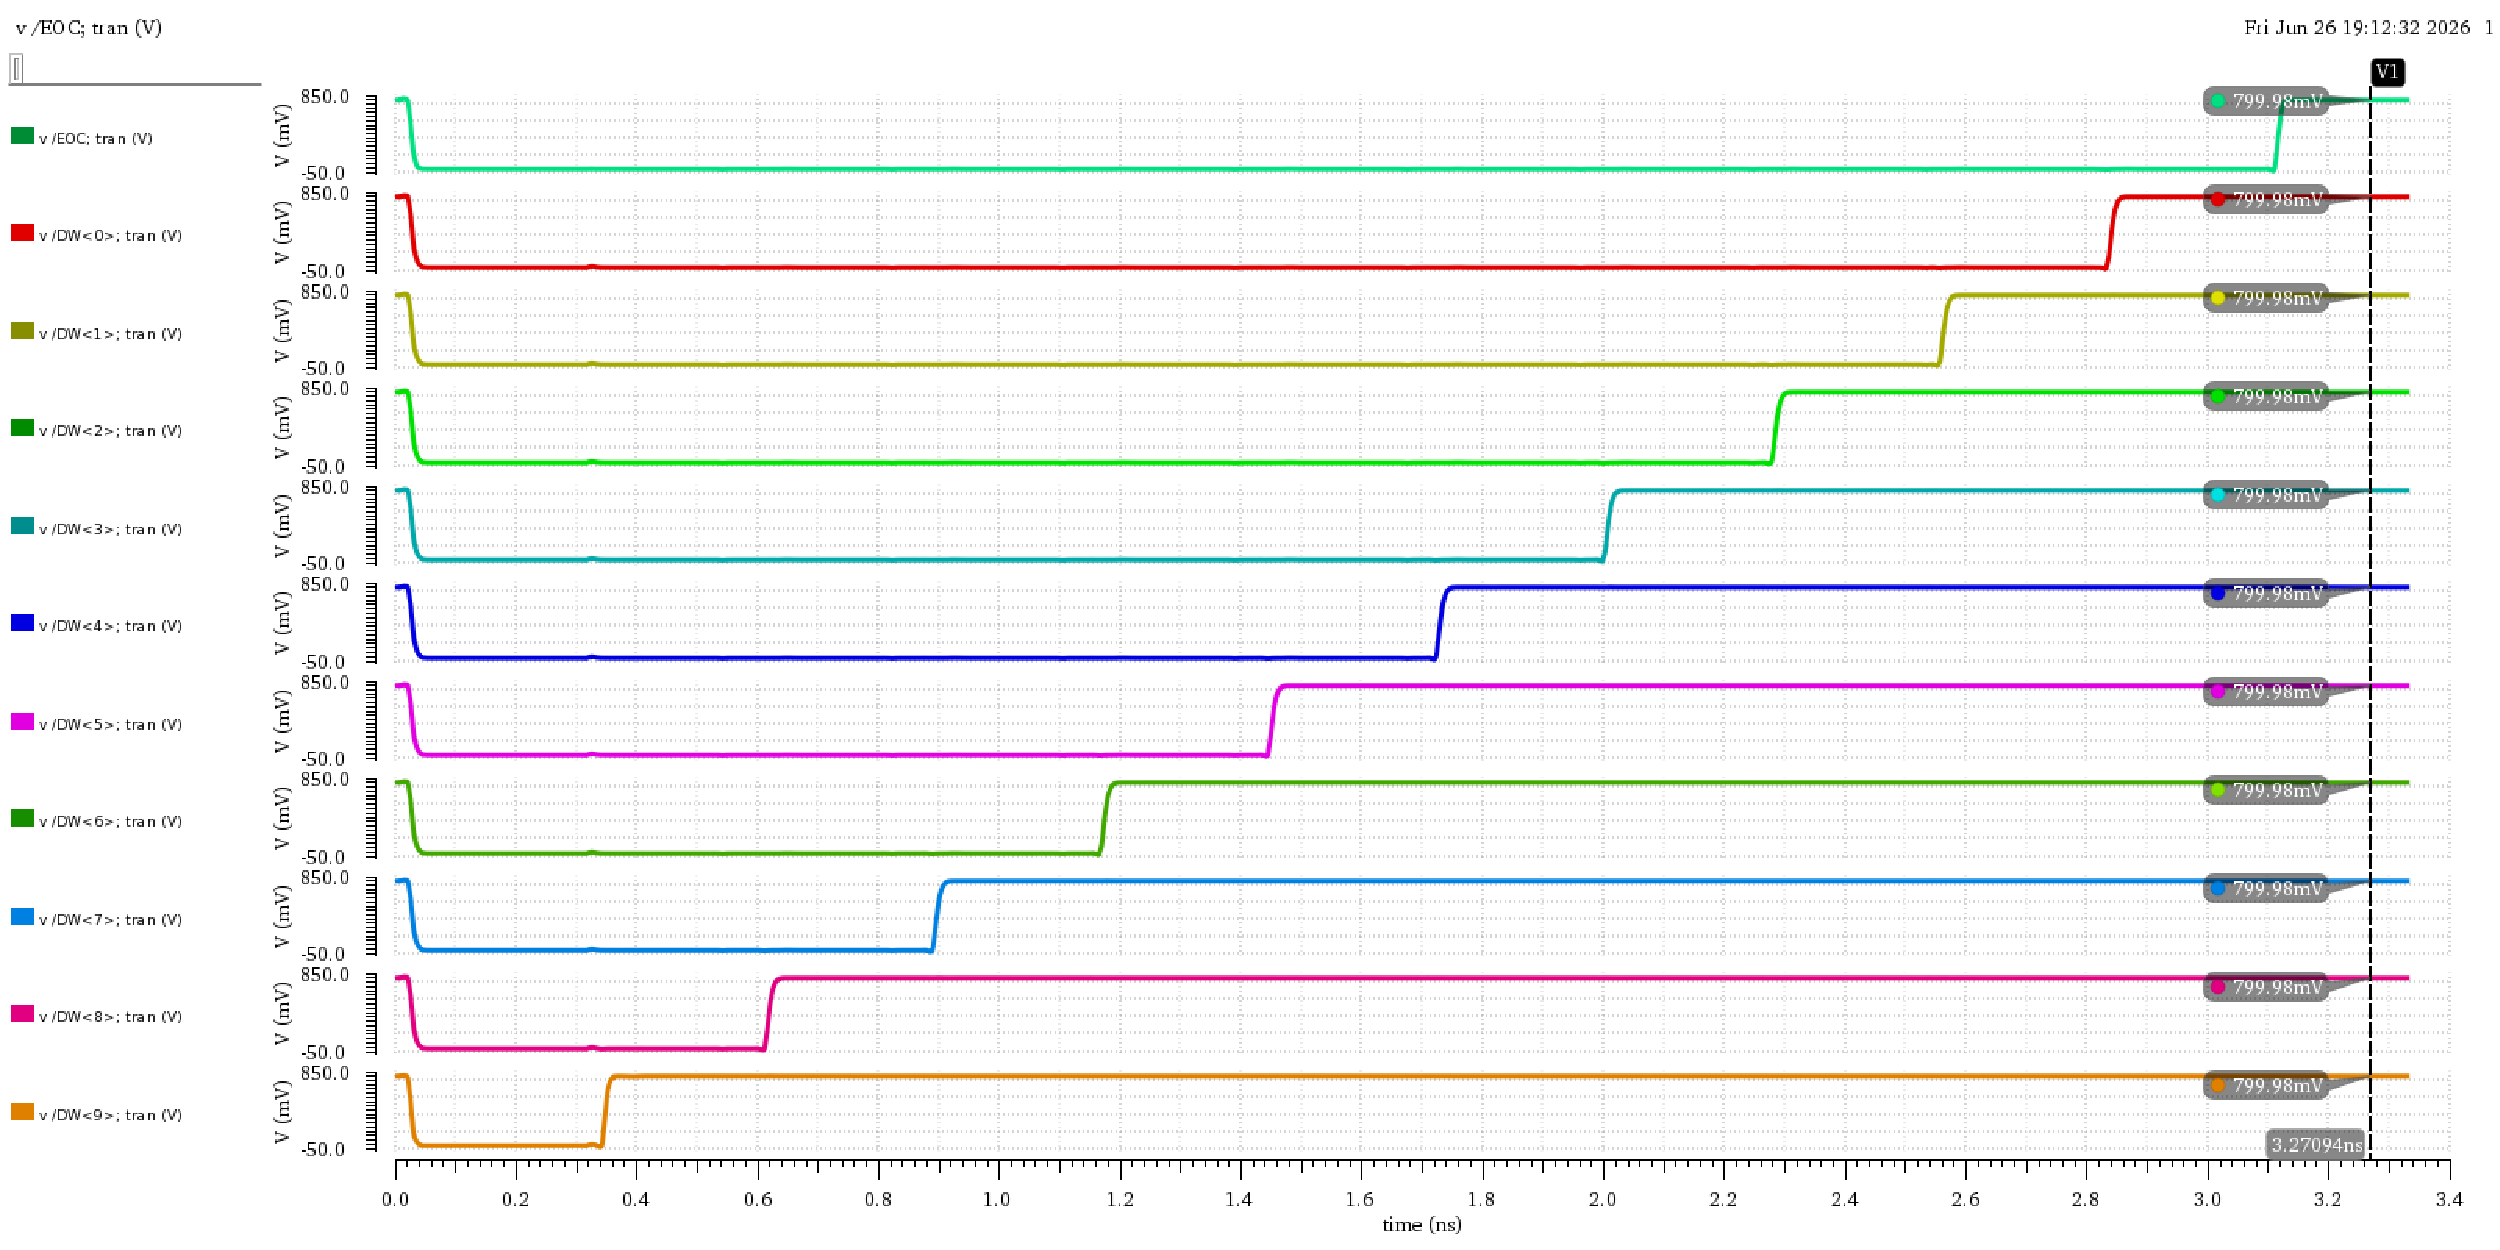
\includegraphics[width=0.75\textwidth]{chapter5/images/21.pdf}
	\caption{Digital output for $V_{\mathrm{in}} = \SI{+800}{mV}$}
	\label{fig:dc_pos800}
\end{figure}

The digital output codes at all three operating points are correct, confirming proper static
operation before proceeding to dynamic testing.

% ══════════════════════════════════════════════════════════════════════════════
\subsection{Ramp Test}


As shown in Fig.~\ref{fig:ramp_slice}, the reconstructed output closely follows the input ramp
with the correct slope across the full input range. The offset observed at the beginning of
the ramp is equal to the on-time of the sampling clock: during the tracking phase the input
continues to increase, so the held value is slightly larger than $\SI{-800}{mV}$ at the
moment the switch opens.

\begin{figure}[h]
	\centering
	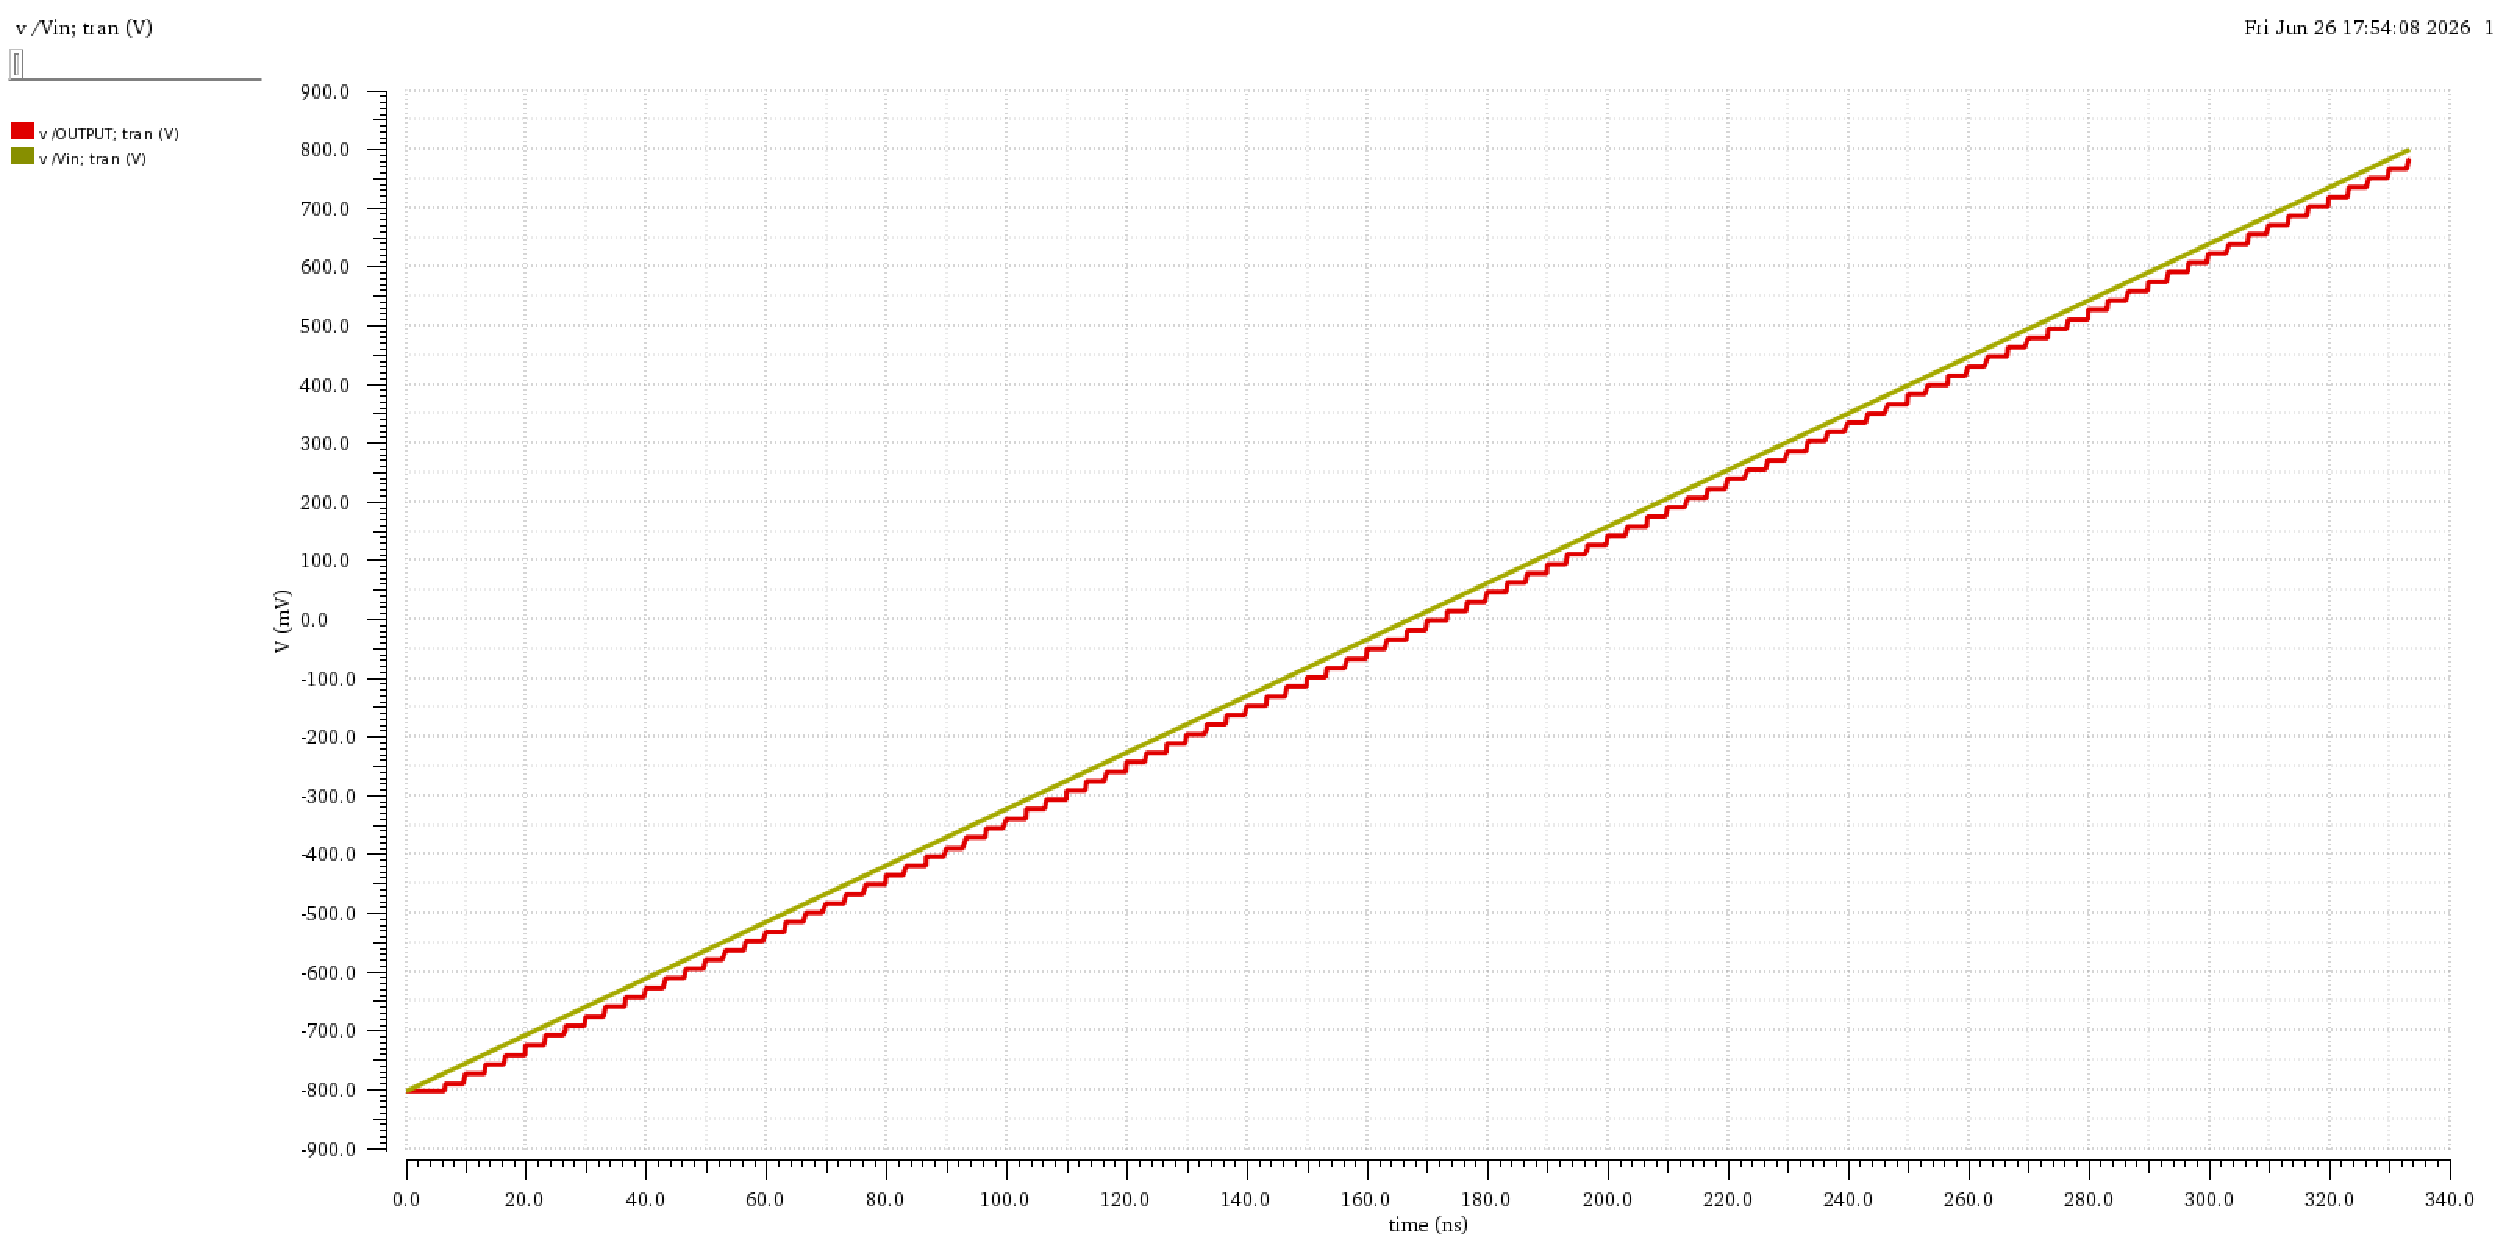
\includegraphics[width=0.8\textwidth]{chapter5/images/22.pdf}
	\caption{Ramp test result for the SAR ADC slice}
	\label{fig:ramp_slice}
\end{figure}


\subsection{Sine Wave Test}
% ══════════════════════════════════════════════════════════════════════════════

The sine wave test requires coherent sampling to be avoided, which is ensured by satisfying

\begin{equation}
	\frac{f_{\mathrm{in}}}{f_s} = \frac{N_{\mathrm{cyc}}}{N_{\mathrm{FFT}}}
\end{equation}

where $N_{\mathrm{cyc}}$ must be a prime number to guarantee that the input frequency is
incoherent with the sampling frequency. For a sampling frequency of \SI{300}{MHz}, $N_{\mathrm{cyc}} = 31$
was selected, yielding an input frequency of approximately \SI{36.3}{MHz}.

\begin{figure}[h!]
	\centering
	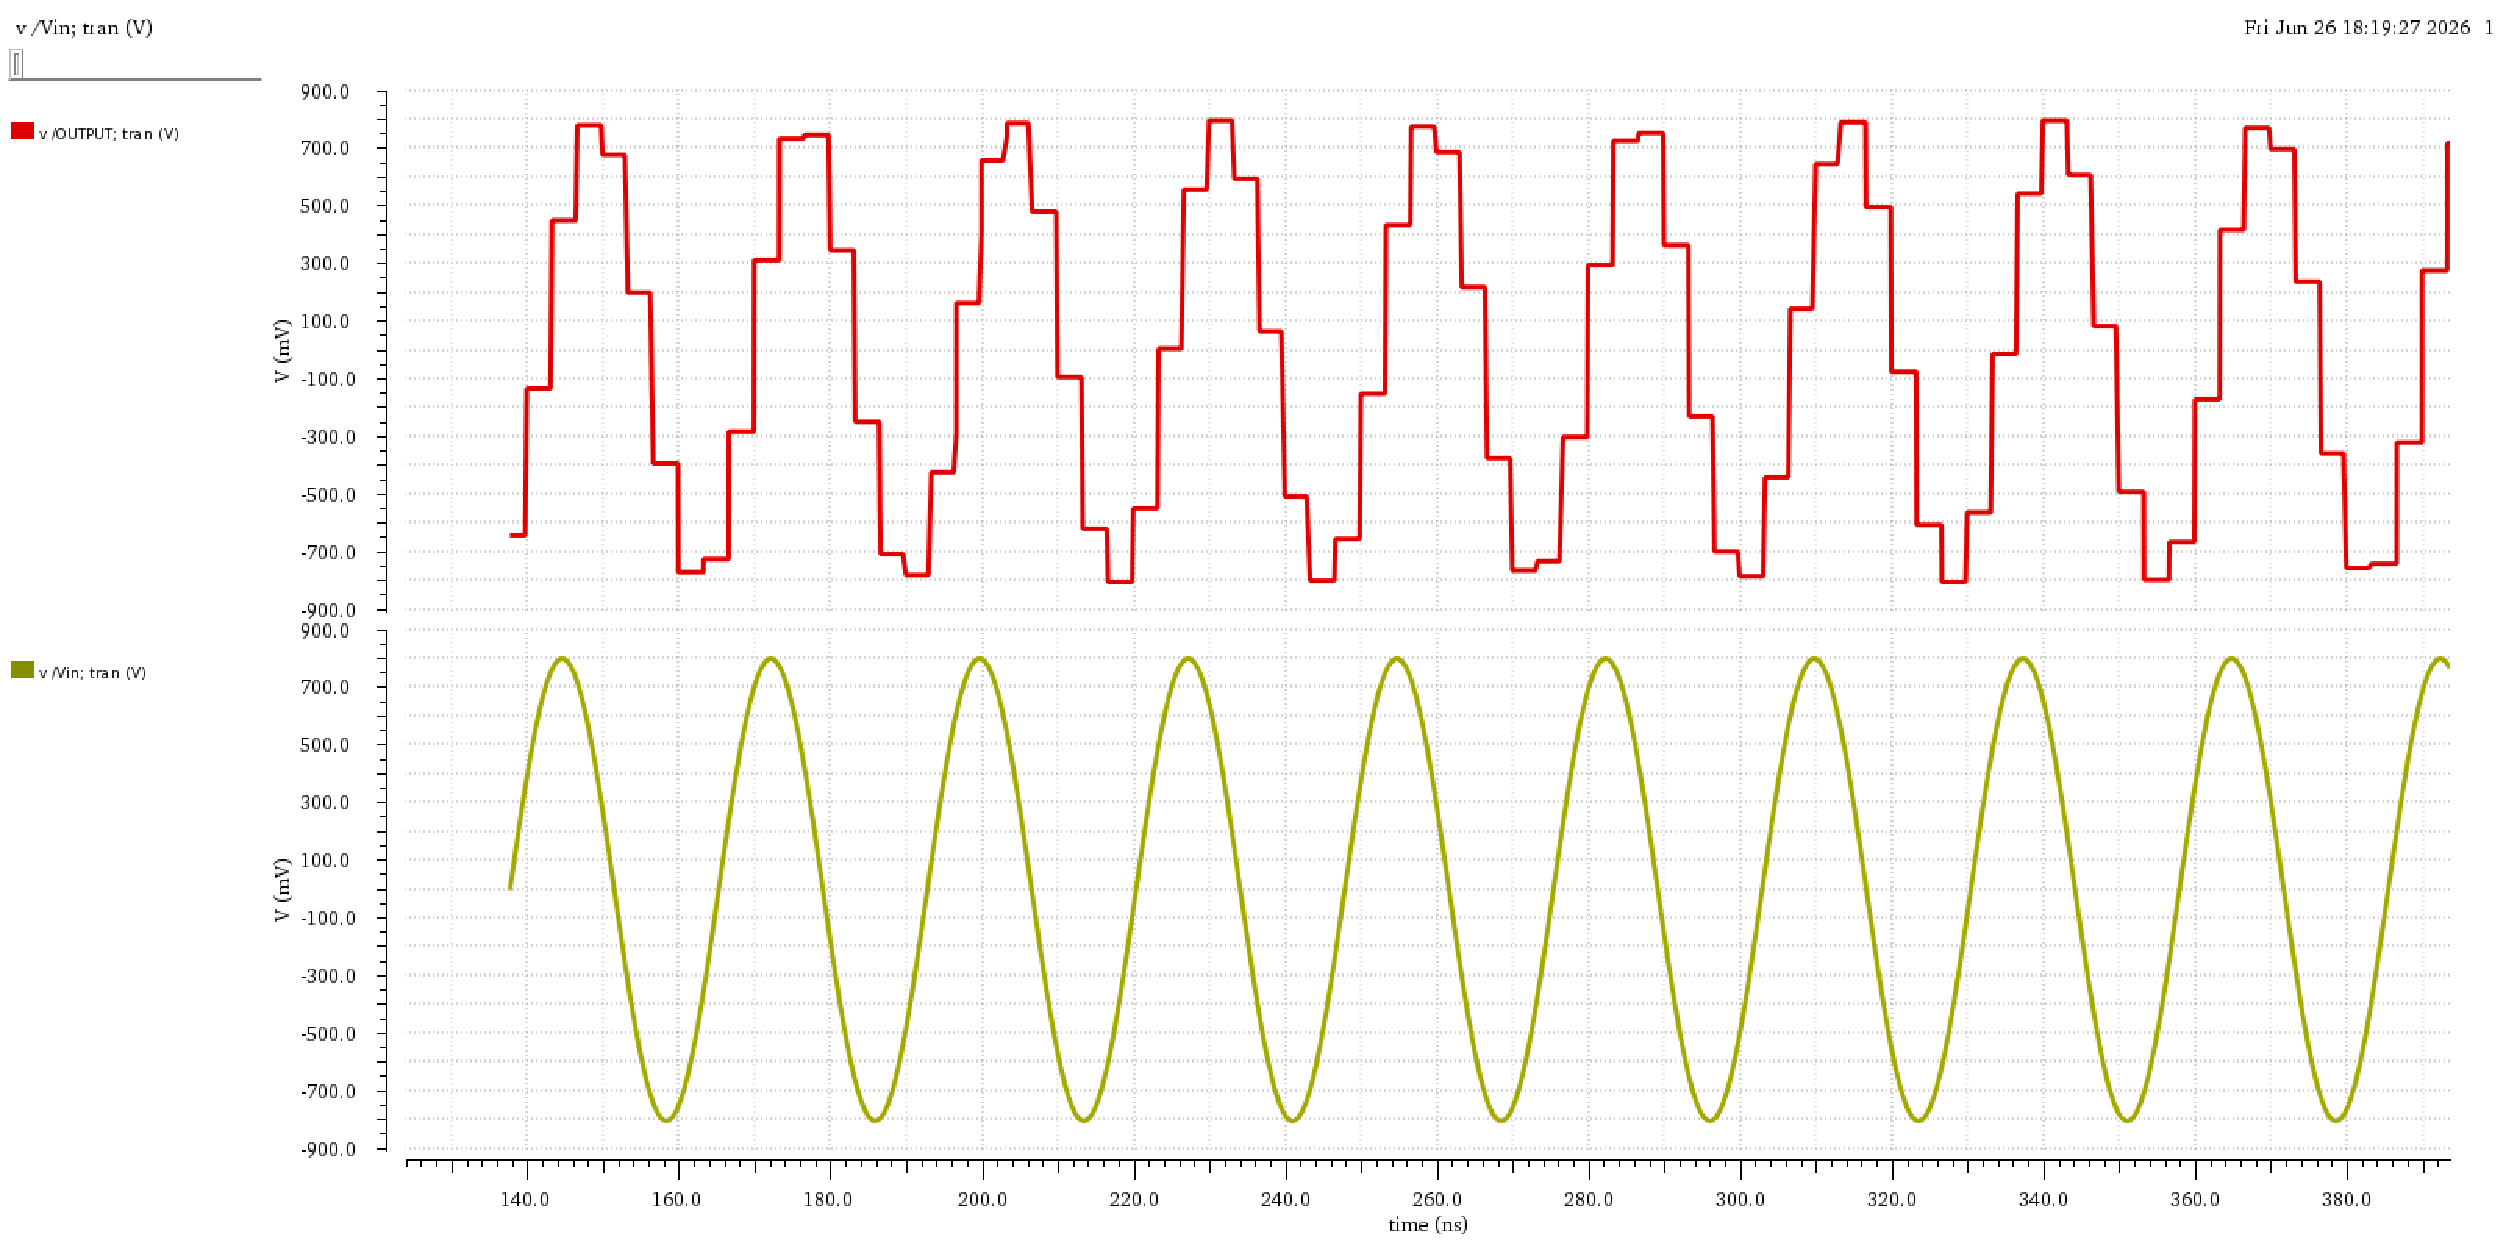
\includegraphics[width=0.8\textwidth]{chapter5/images/23.pdf}
	\caption{Reconstructed output from the ideal DAC}
	\label{fig:ideal_dac_out}
\end{figure}

\begin{figure}[h!]
	\centering
	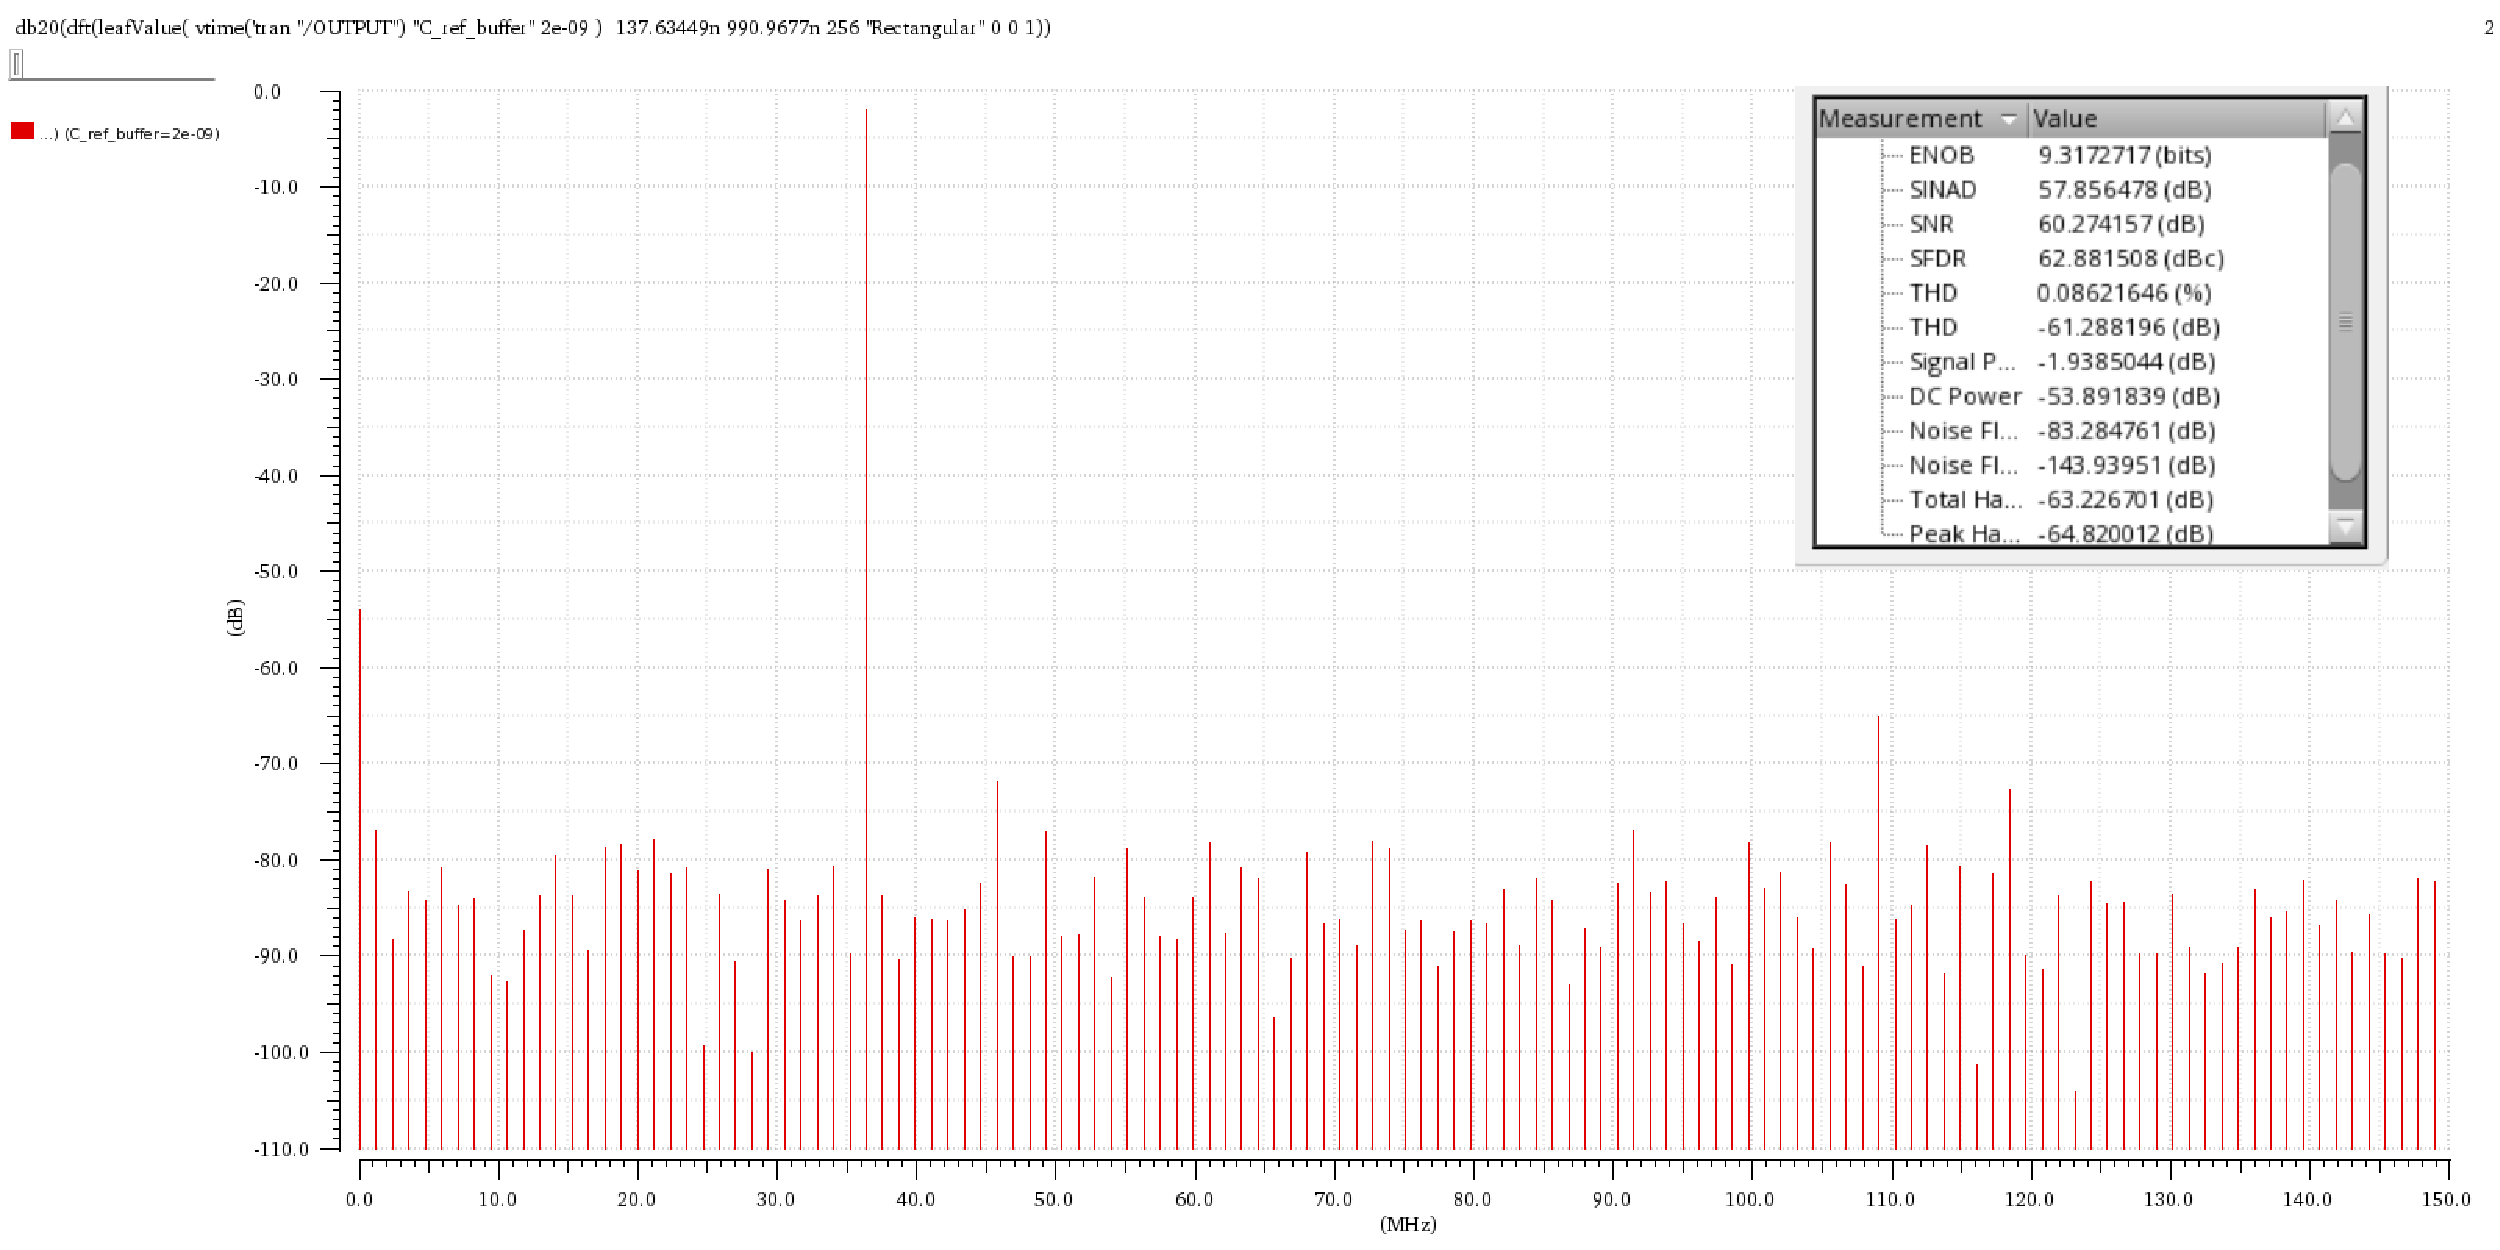
\includegraphics[width=0.8\textwidth]{chapter5/images/24.pdf}
	\caption{FFT of the ideal DAC output for the single-slice SAR ADC}
	\label{fig:fft_slice}
\end{figure}

As shown in Fig.~\ref{fig:ideal_dac_out}, the reconstructed output accurately tracks the
input and reaches both reference levels ($V_{\mathrm{REFP}}$ and $V_{\mathrm{REFN}}$). The
FFT in Fig.~\ref{fig:fft_slice} shows a noise floor of \SI{-83}{dB}. The third harmonic is
the dominant distortion component, limiting the SFDR to approximately \SI{63}{dB}. The
achieved ENOB is \textbf{9.3 bits}, which is a strong result for a 10-bit ADC operating at
this conversion rate.


\section{Time-Interleaved SAR ADC Integration}
% ══════════════════════════════════════════════════════════════════════════════

The time-interleaved (TI) ADC is constructed from 8 identical \SI{300}{MHz} SAR ADC slices,
yielding an aggregate sampling rate of \SI{2.4}{GHz}. The sampling instants must be uniformly
distributed in time; each successive slice is delayed by $1/(8 f_s) = \SI{416.7}{ps}$
relative to its predecessor. The sampling clock pulse width was set to $1/(11 f_s)$ to
provide adequate settling margin within each interleaving period.

\begin{figure}[h!]
	\centering
	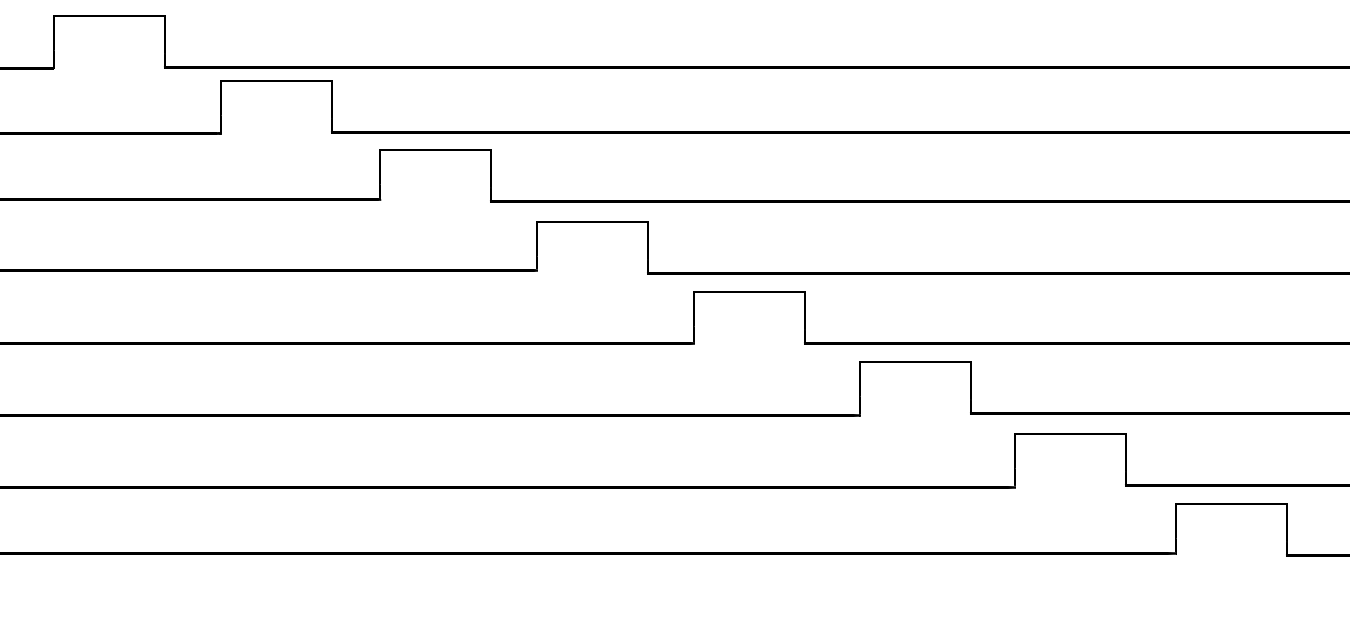
\includegraphics[width=0.7\textwidth]{chapter5/images/25.png}
	\caption{Sampling clock phases for the 8-channel TI SAR ADC}
	\label{fig:ti_clocks}
\end{figure}

The analog input is distributed to all eight slices through a dedicated input buffer per
channel. Due to time constraints, ideal buffer models were used in this work; the design of
physical input buffers is identified as future work.

\begin{figure}[h!]
	\centering
	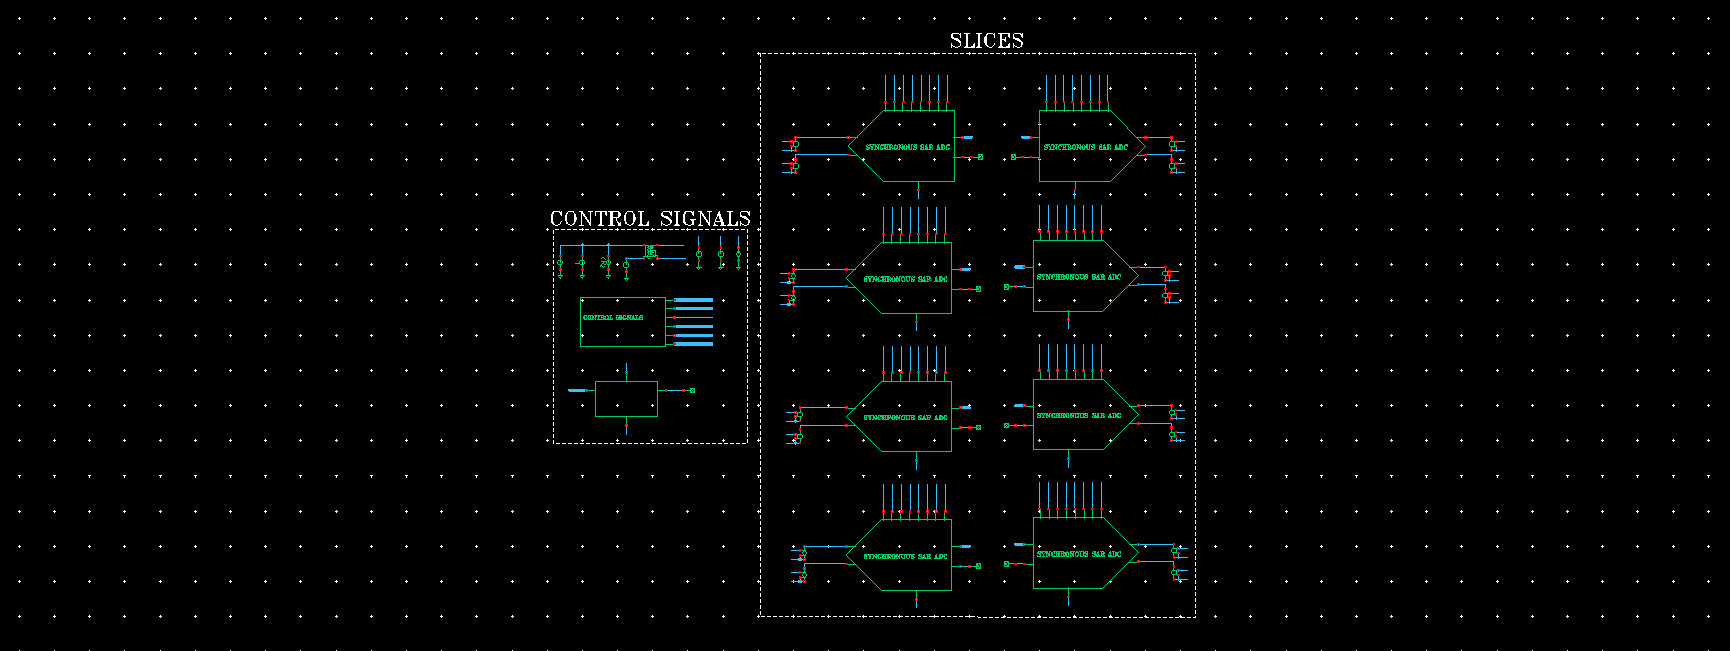
\includegraphics[width=0.9\textwidth]{chapter5/images/26.png}
	\caption{Top-level schematic of the TI SAR ADC}
	\label{fig:ti_schematic}
\end{figure}

\begin{figure}[h!]
	\centering
	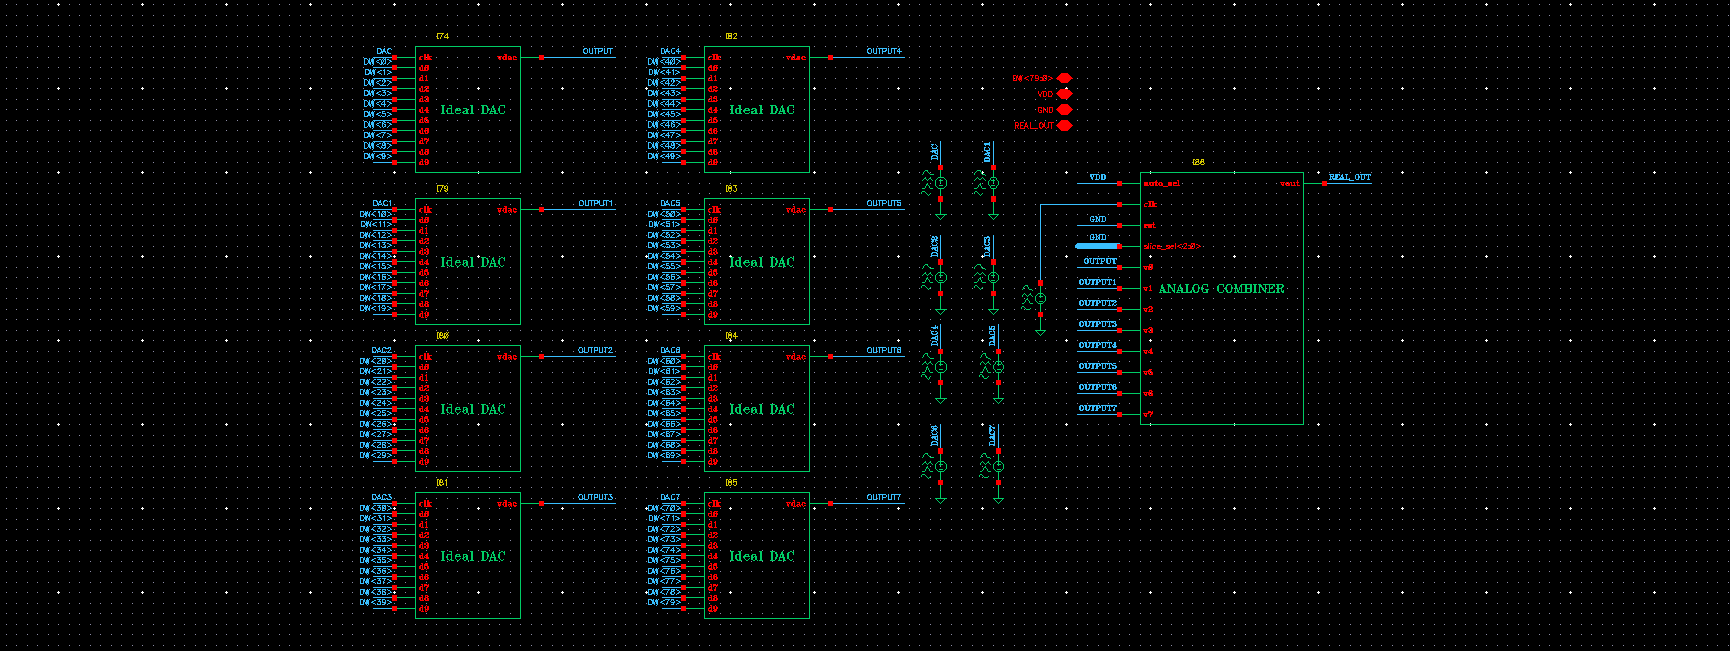
\includegraphics[width=0.9\textwidth]{chapter5/images/27.png}
	\caption{Ideal DAC model used for output reconstruction}
	\label{fig:ti_ideal_dac}
\end{figure}

\subsection{Ramp Test}
Compared to the single-slice ramp in Fig.~\ref{fig:ramp_slice}, the TI ramp in
Fig.~\ref{fig:ti_ramp} is noticeably smoother. The effective sampling interval is reduced from
\SI{3.3}{ns} to \SI{417}{ps}, producing a finer output staircase that closely approximates
the input ramp across the full range.
\newpage
\begin{figure}[h!]
	\centering
	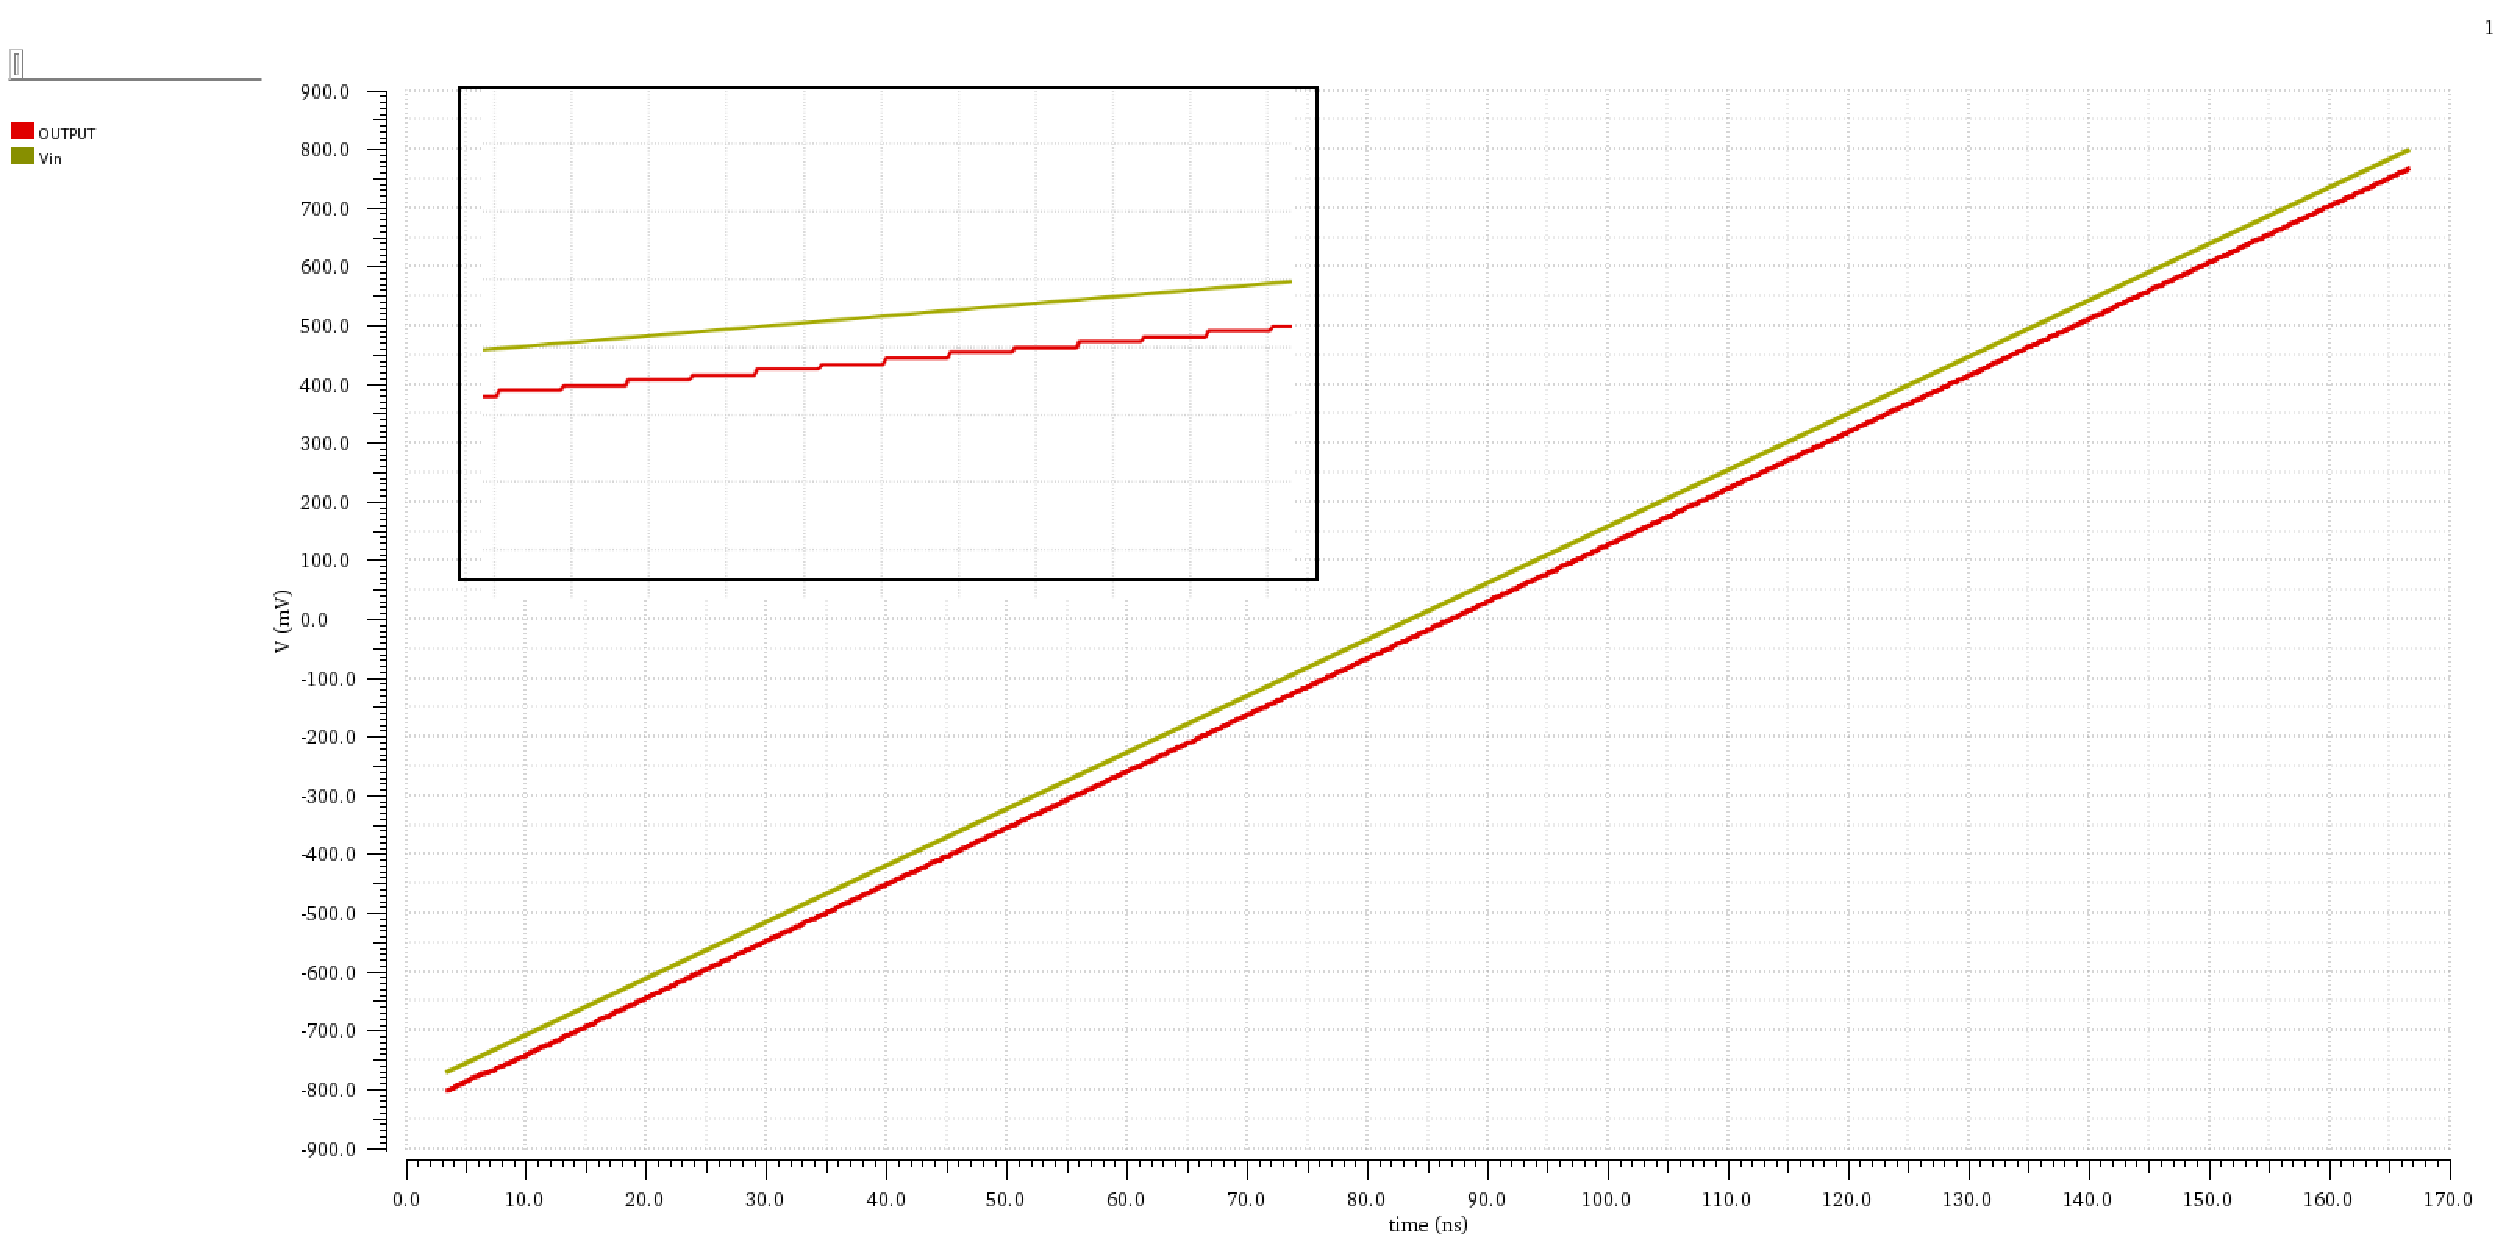
\includegraphics[width=0.8\textwidth]{chapter5/images/28.pdf}
	\caption{Ramp test result for the TI SAR ADC}
	\label{fig:ti_ramp}
\end{figure}



\subsection{Sine Wave Test}

The sine wave test was performed across multiple input frequencies to characterise the
frequency-dependent performance of the TI ADC.

\begin{figure}[h!]
	\centering
	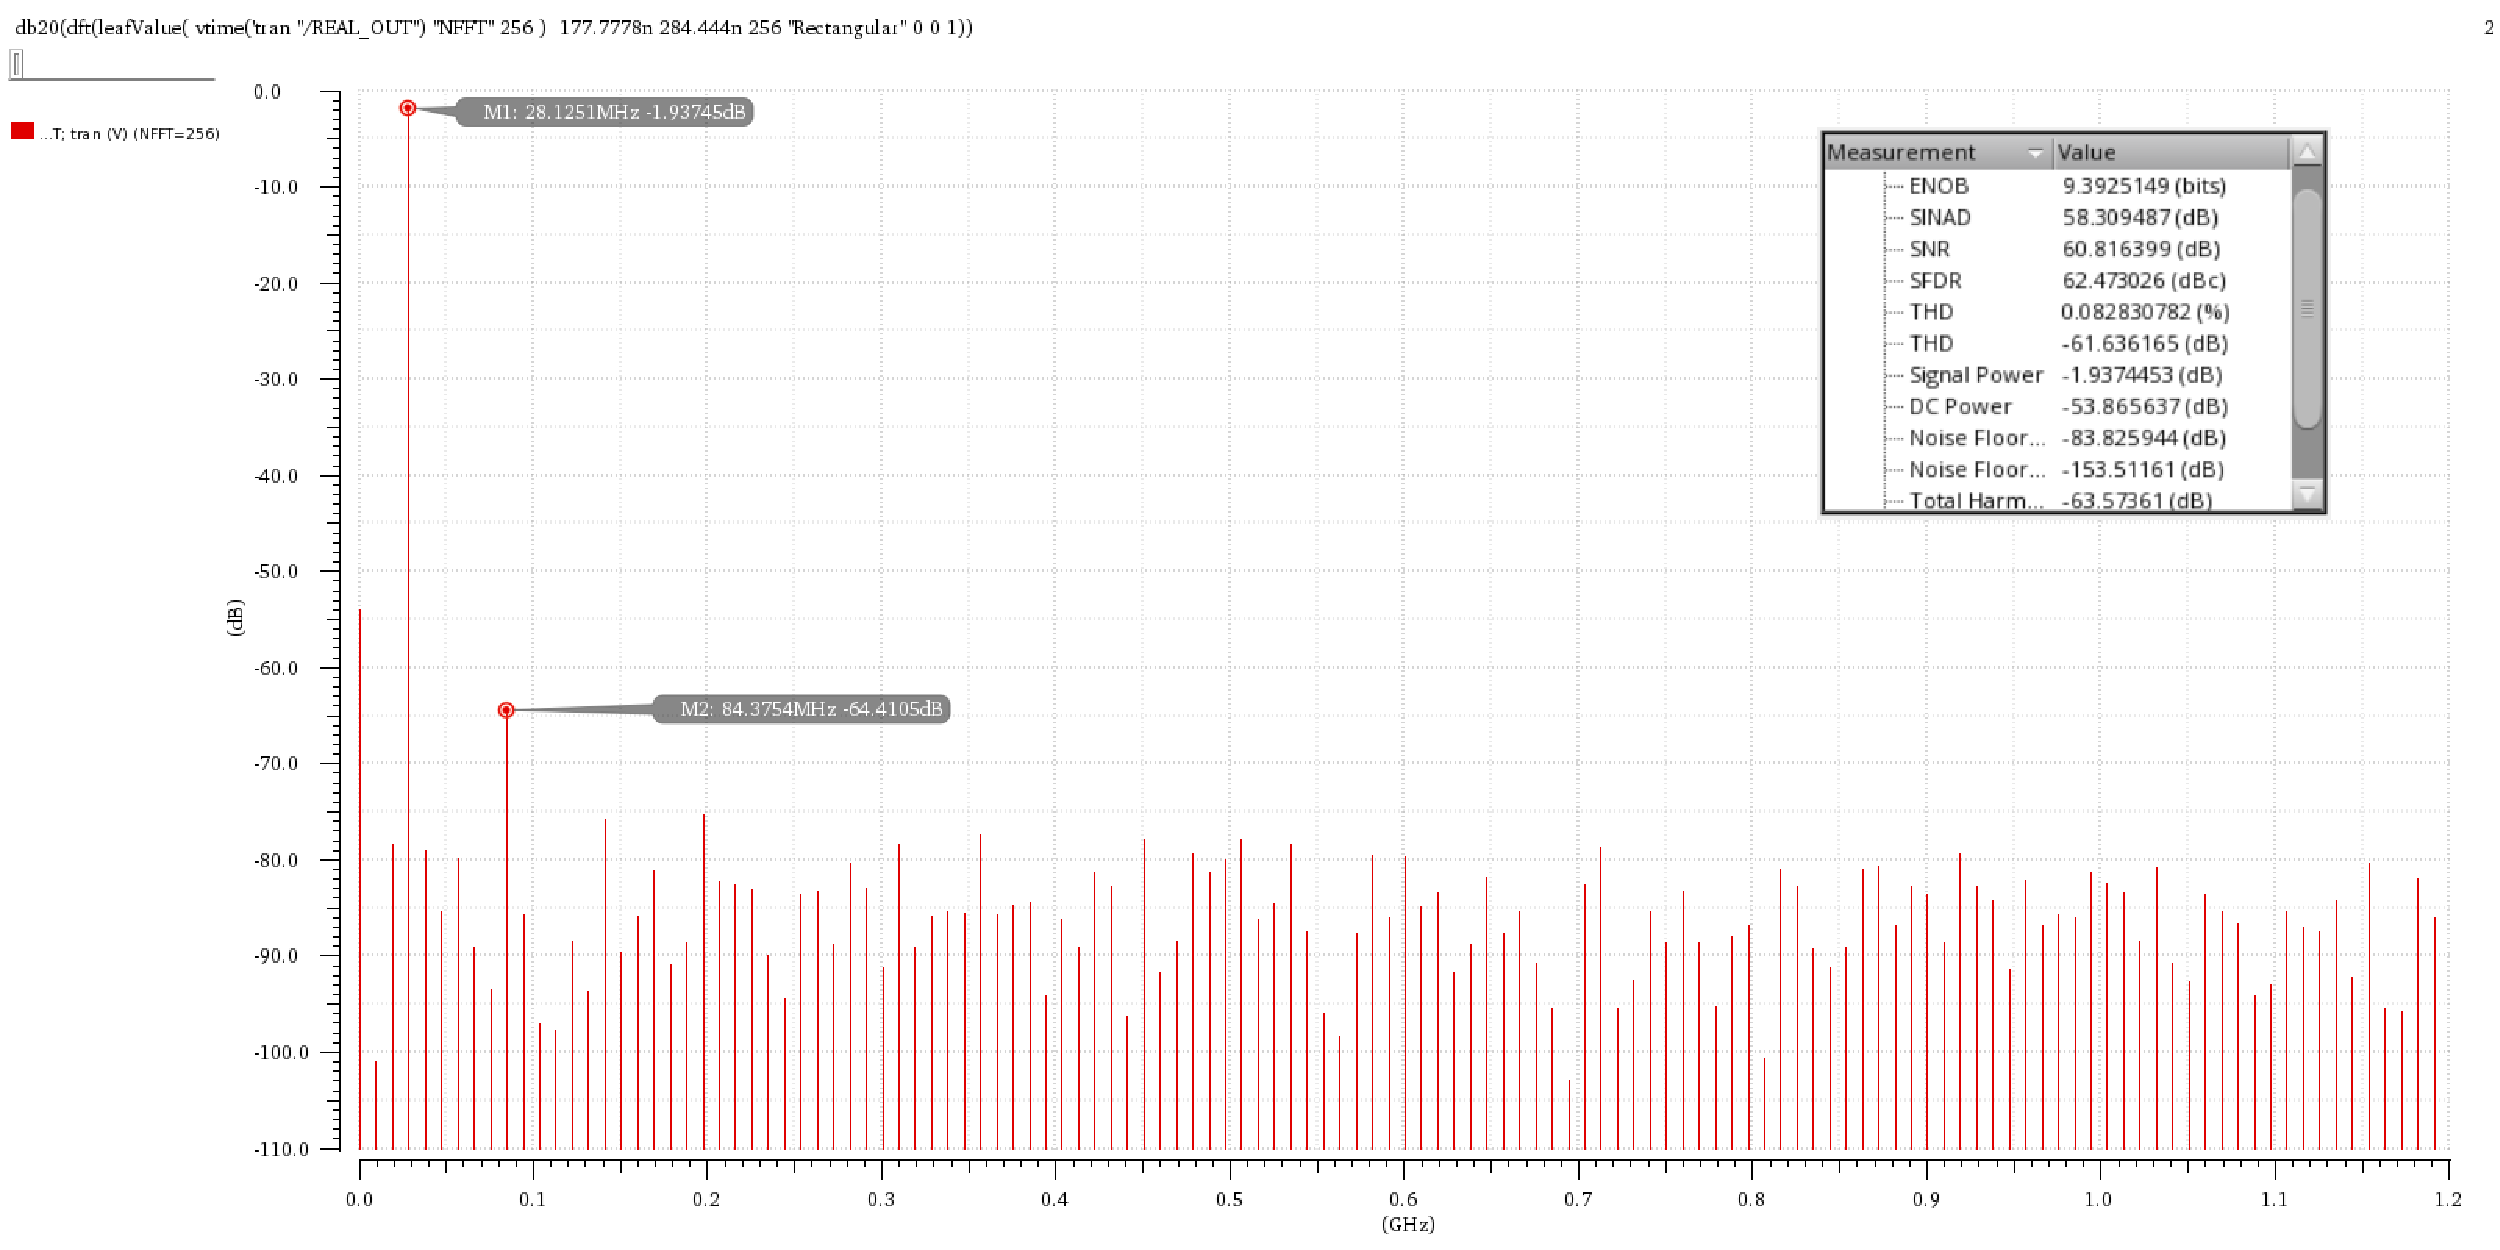
\includegraphics[width=0.75\textwidth]{chapter5/images/29.pdf}
	\caption{FFT of the ideal DAC output at $f_{\mathrm{in}} = \SI{28}{MHz}$ (typical corner)}
	\label{fig:ti_fft_28mhz}
\end{figure}

\begin{figure}[h!]
	\centering
	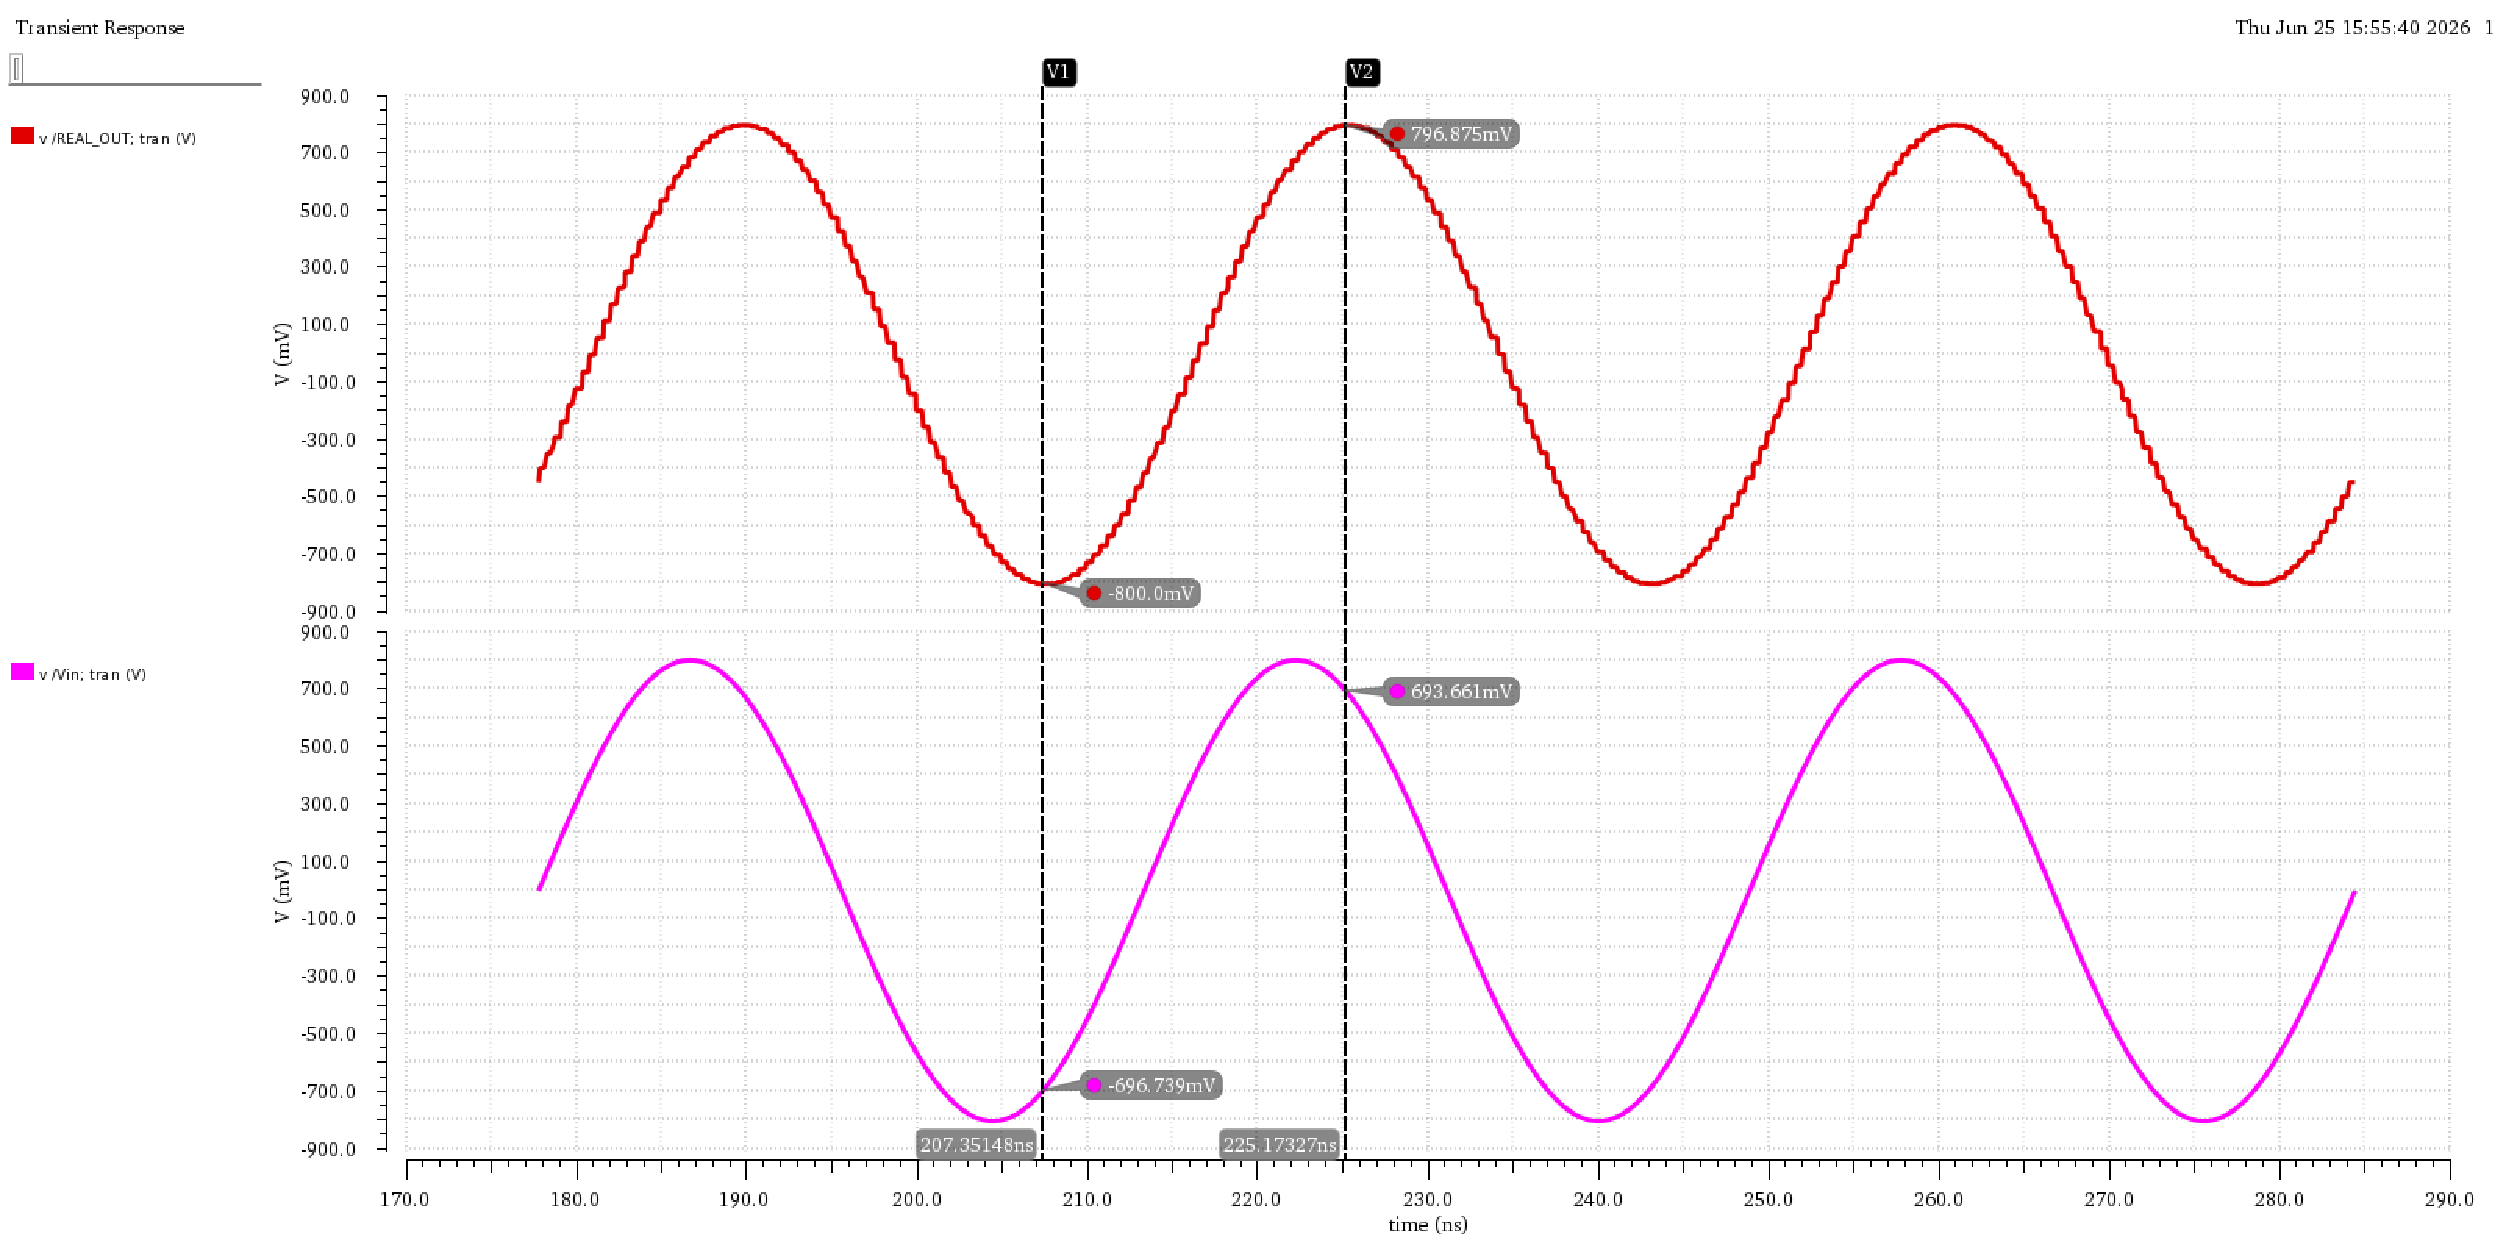
\includegraphics[width=0.7\textwidth]{chapter5/images/30.pdf}
	\caption{Reconstructed sine wave from the ideal DAC at low input frequency}
	\label{fig:ti_sine_out}
\end{figure}

The reconstructed waveform in Fig.~\ref{fig:ti_sine_out} is significantly smoother than the
single-slice result, reaching both $V_{\mathrm{REFP}}$ and $V_{\mathrm{REFN}}$ across the
full \SI{1.6}{V} differential range.

\begin{figure}[h!]
	\centering
	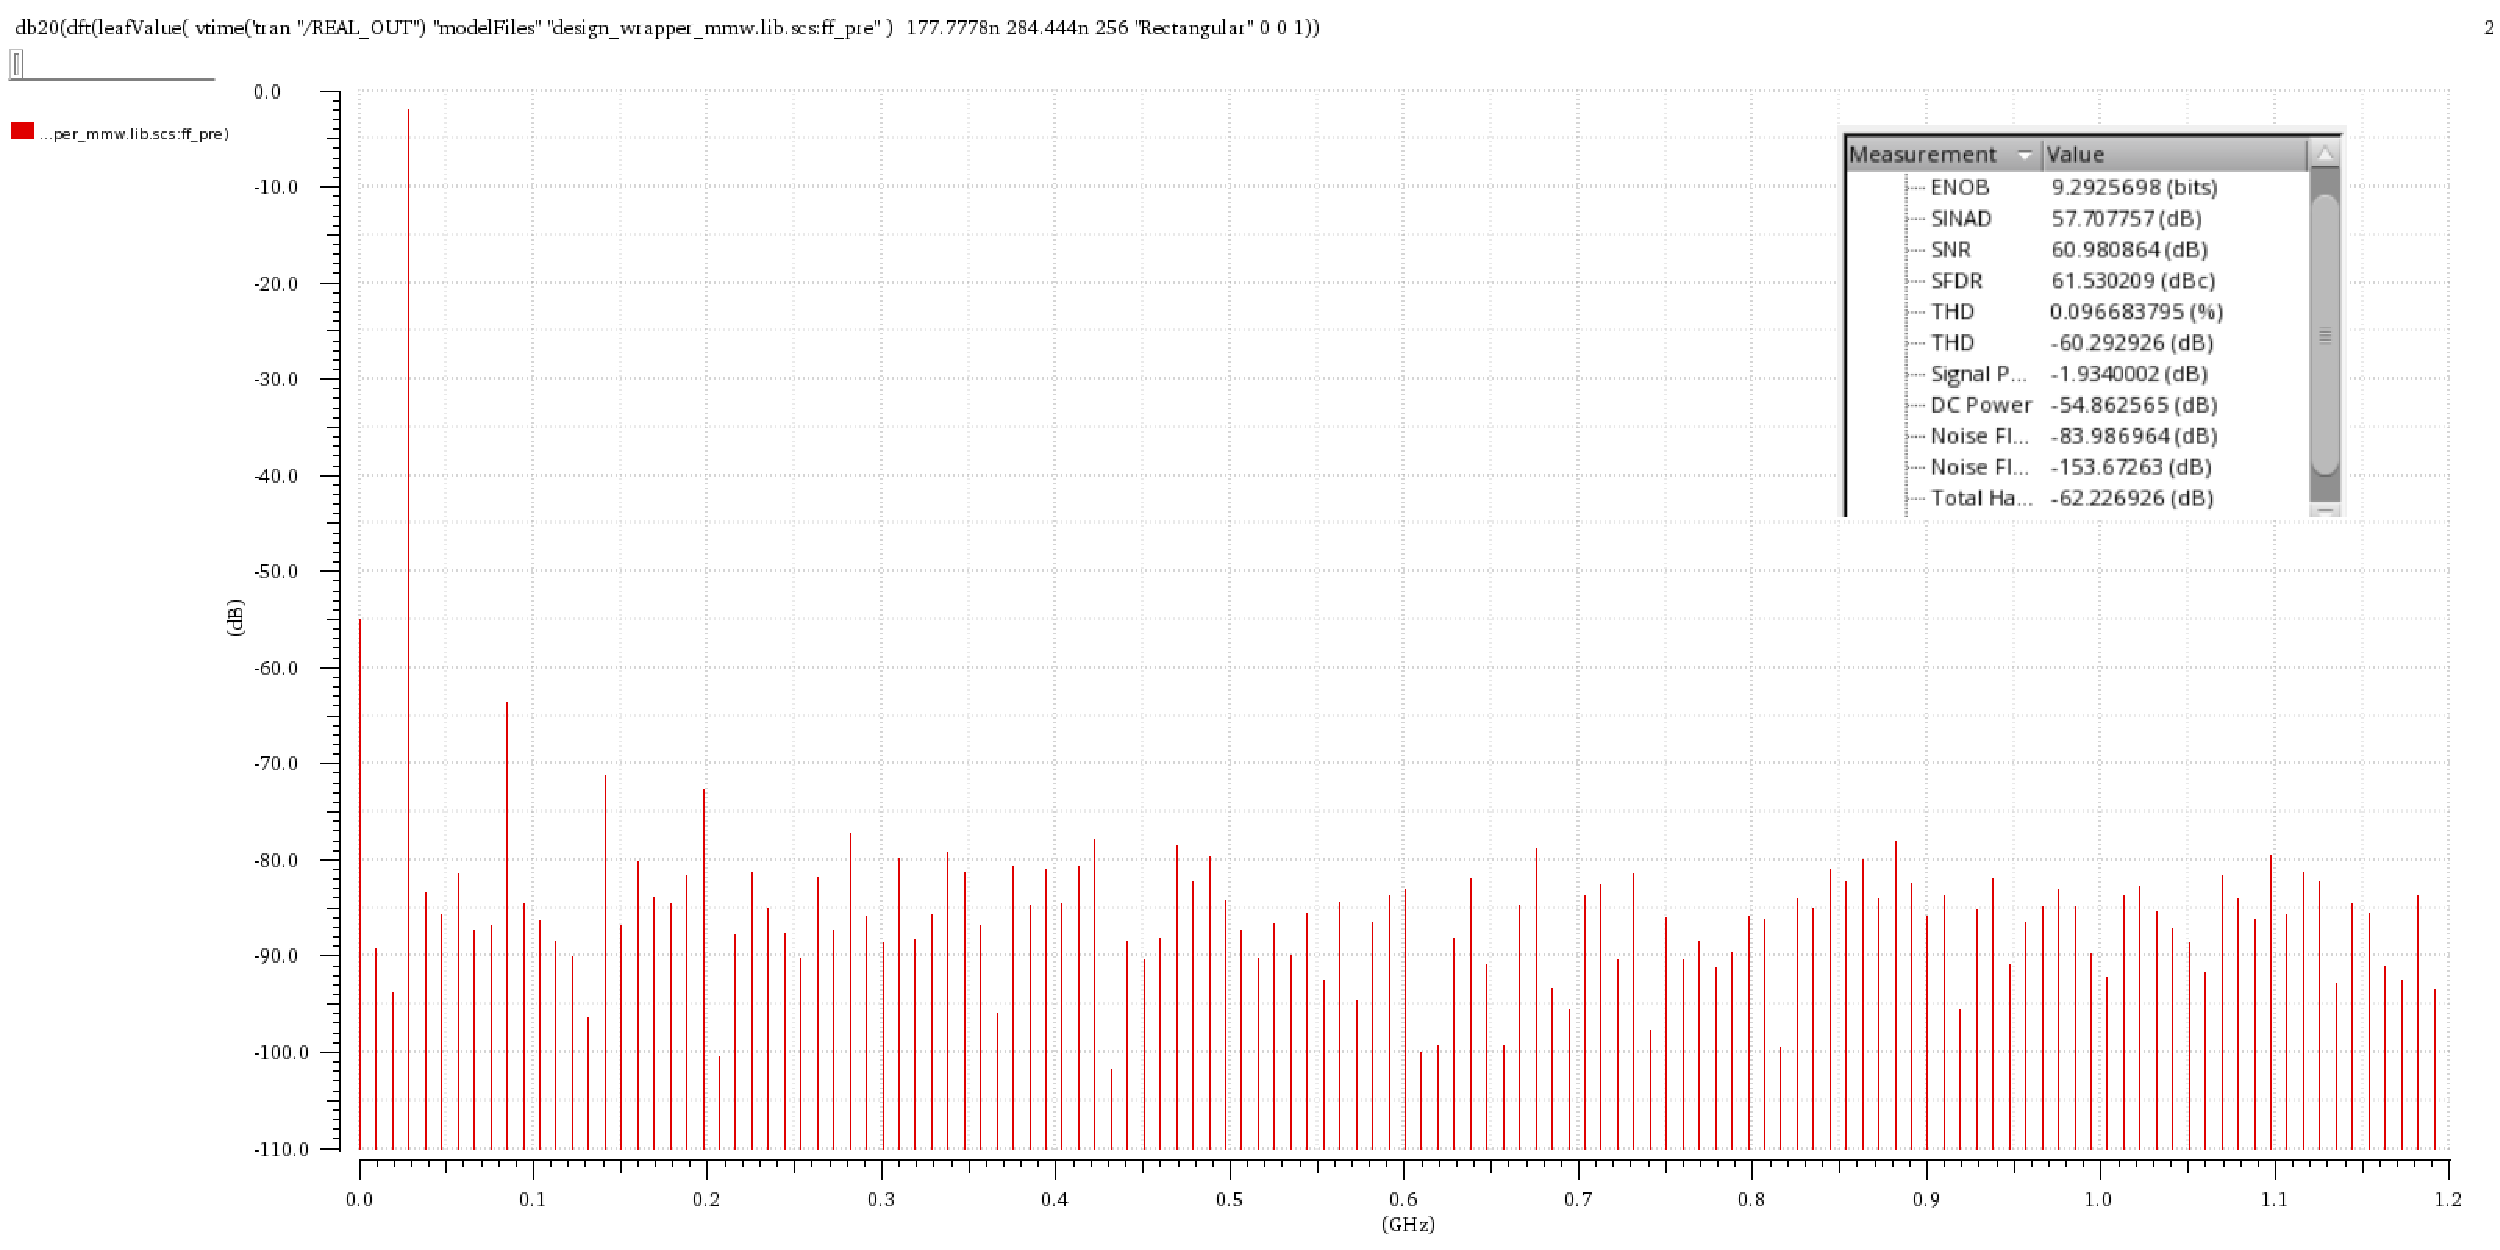
\includegraphics[width=0.8\textwidth]{chapter5/images/31.pdf}
	\caption{FFT output at FF corner (\SI{-40}{\celsius})}
	\label{fig:ti_fft_ff}
\end{figure}

\begin{figure}[h!]
	\centering
	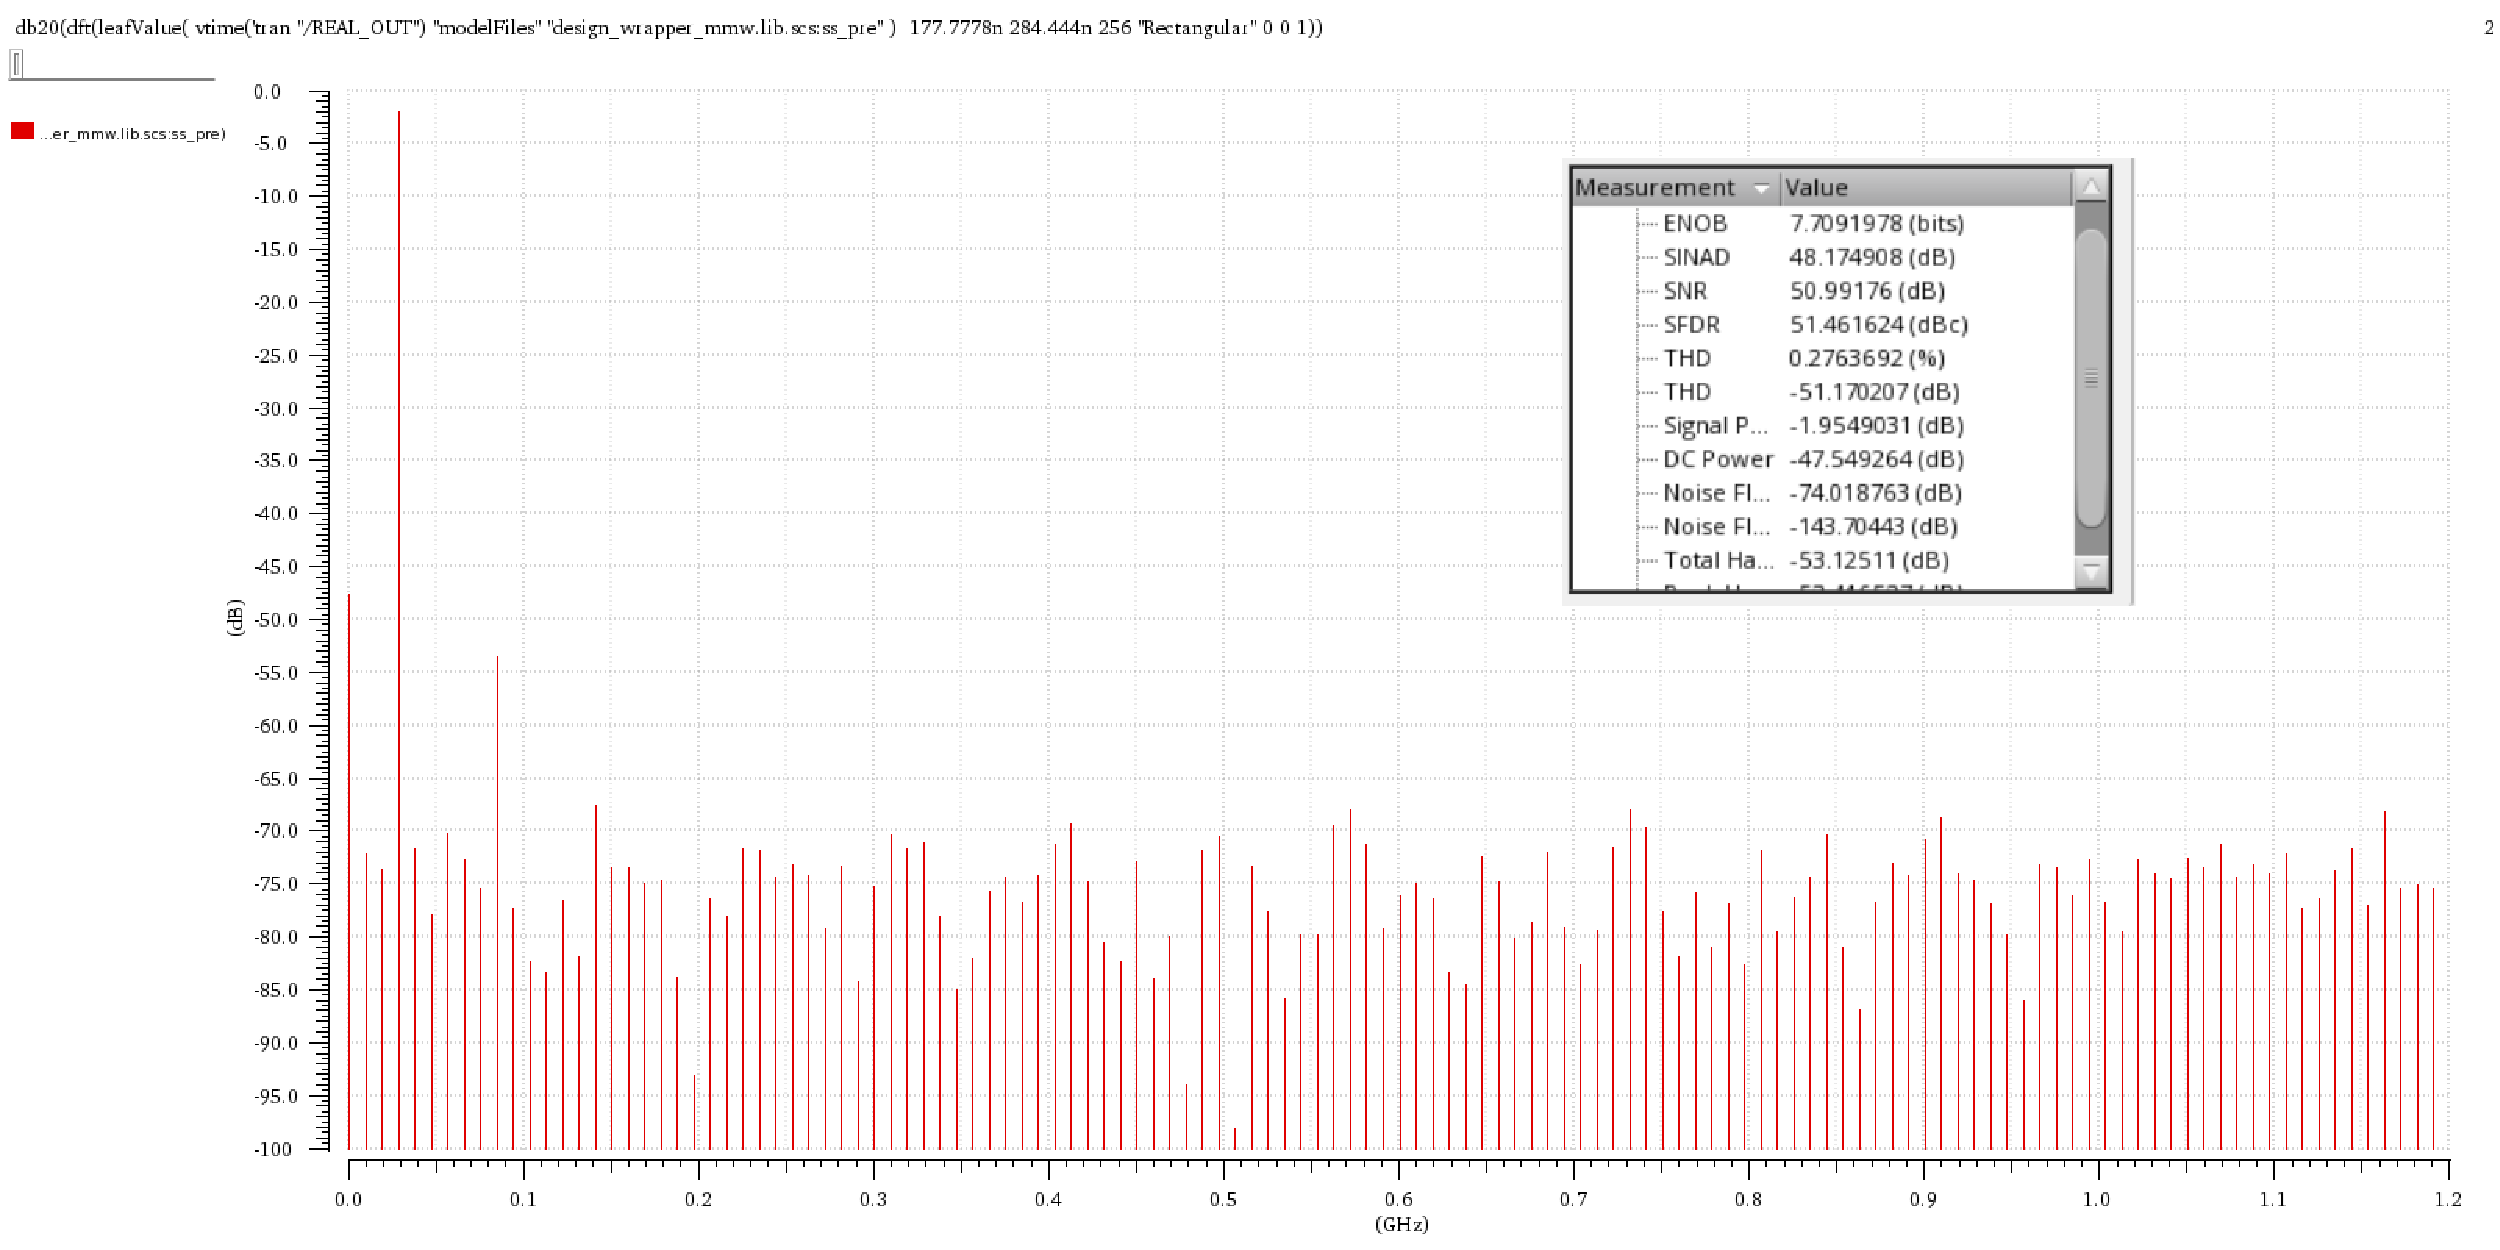
\includegraphics[width=0.8\textwidth]{chapter5/images/32.pdf}
	\caption{FFT output at SS corner (\SI{125}{\celsius})}
	\label{fig:ti_fft_ss}
\end{figure}

At the FF corner (Fig.~\ref{fig:ti_fft_ff}), the ENOB and other metrics remain close to the
typical values. At the SS corner (Fig.~\ref{fig:ti_fft_ss}), the ENOB degrades significantly
to \textbf{7.7 bits} from the typical value of \textbf{9.4 bits}. This degradation is
attributed to the slow switching speed of the input sampling switches in the SS corner.
Increasing the switch width beyond the chosen value was found to be counterproductive: the
resulting increase in off-state leakage caused the ENOB to drop further to approximately
5 bits. The selected sizing therefore represents the optimum trade-off between on-resistance
and leakage current in this process corner.

\begin{figure}[h!]
	\centering
	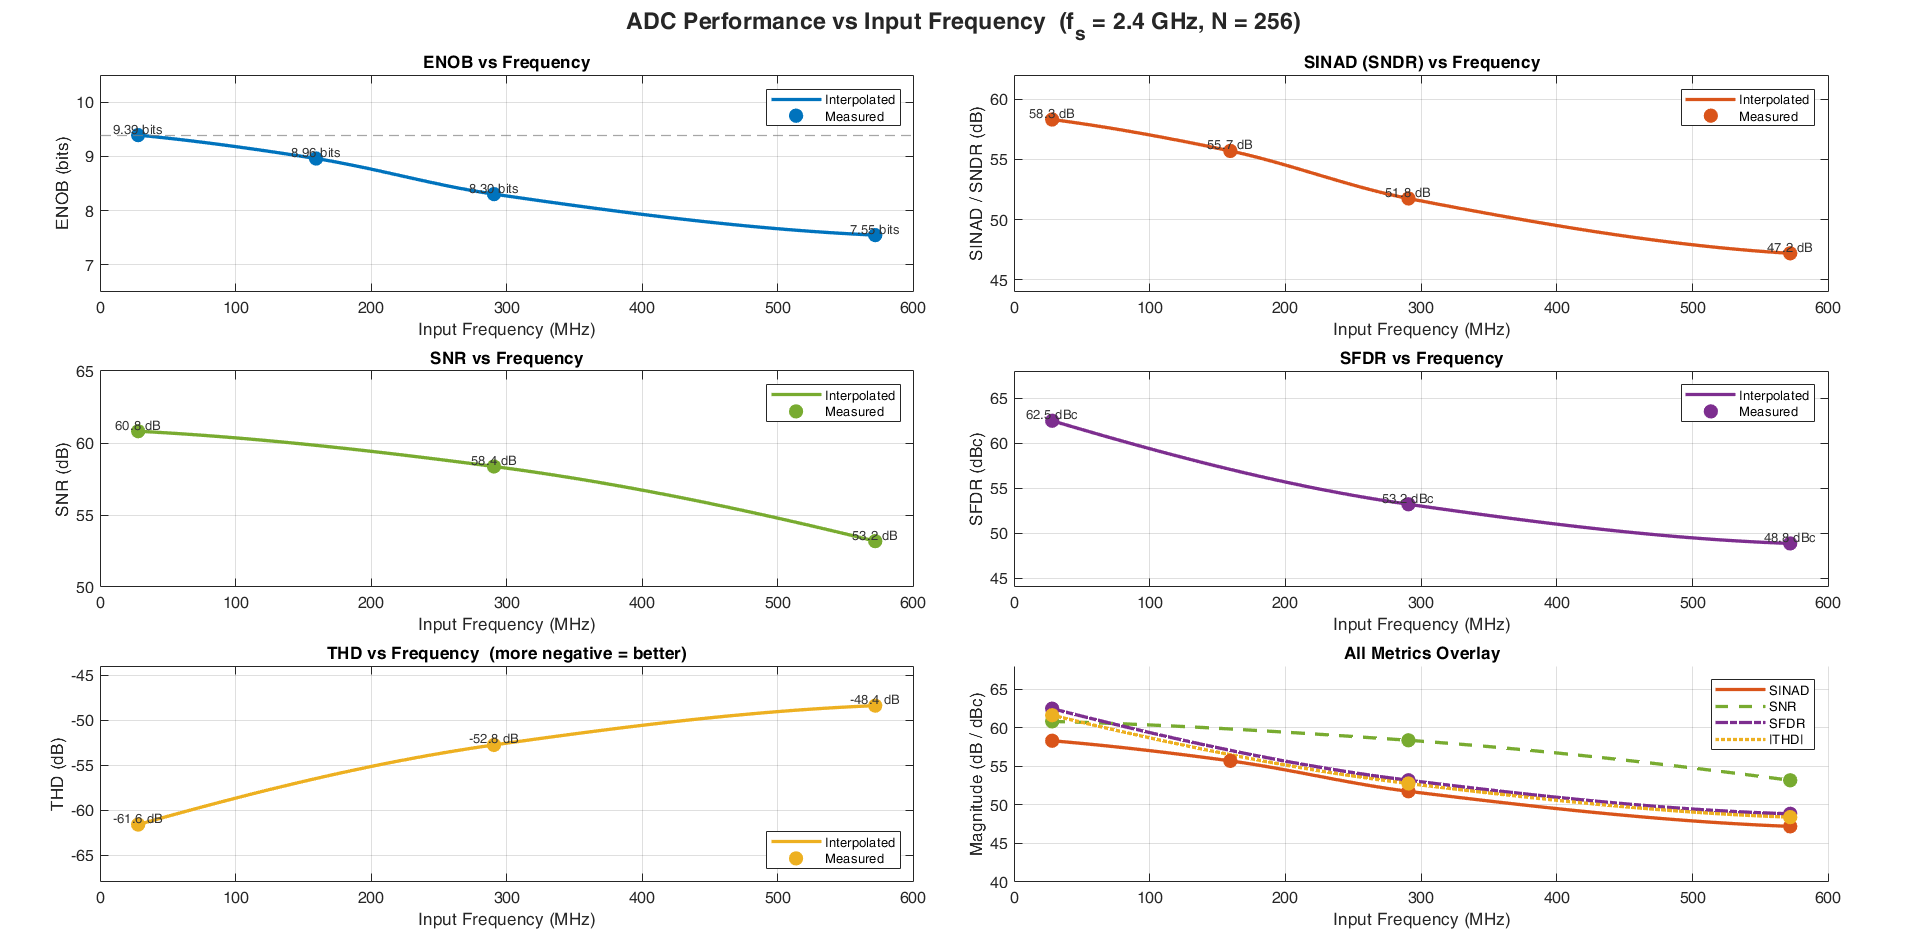
\includegraphics[width=0.95\textwidth]{chapter5/images/33.png}
	\caption{Key ADC metrics vs.\ input frequency --- typical corner}
	\label{fig:metrics_typ}
\end{figure}

\begin{figure}[h!]
	\centering
	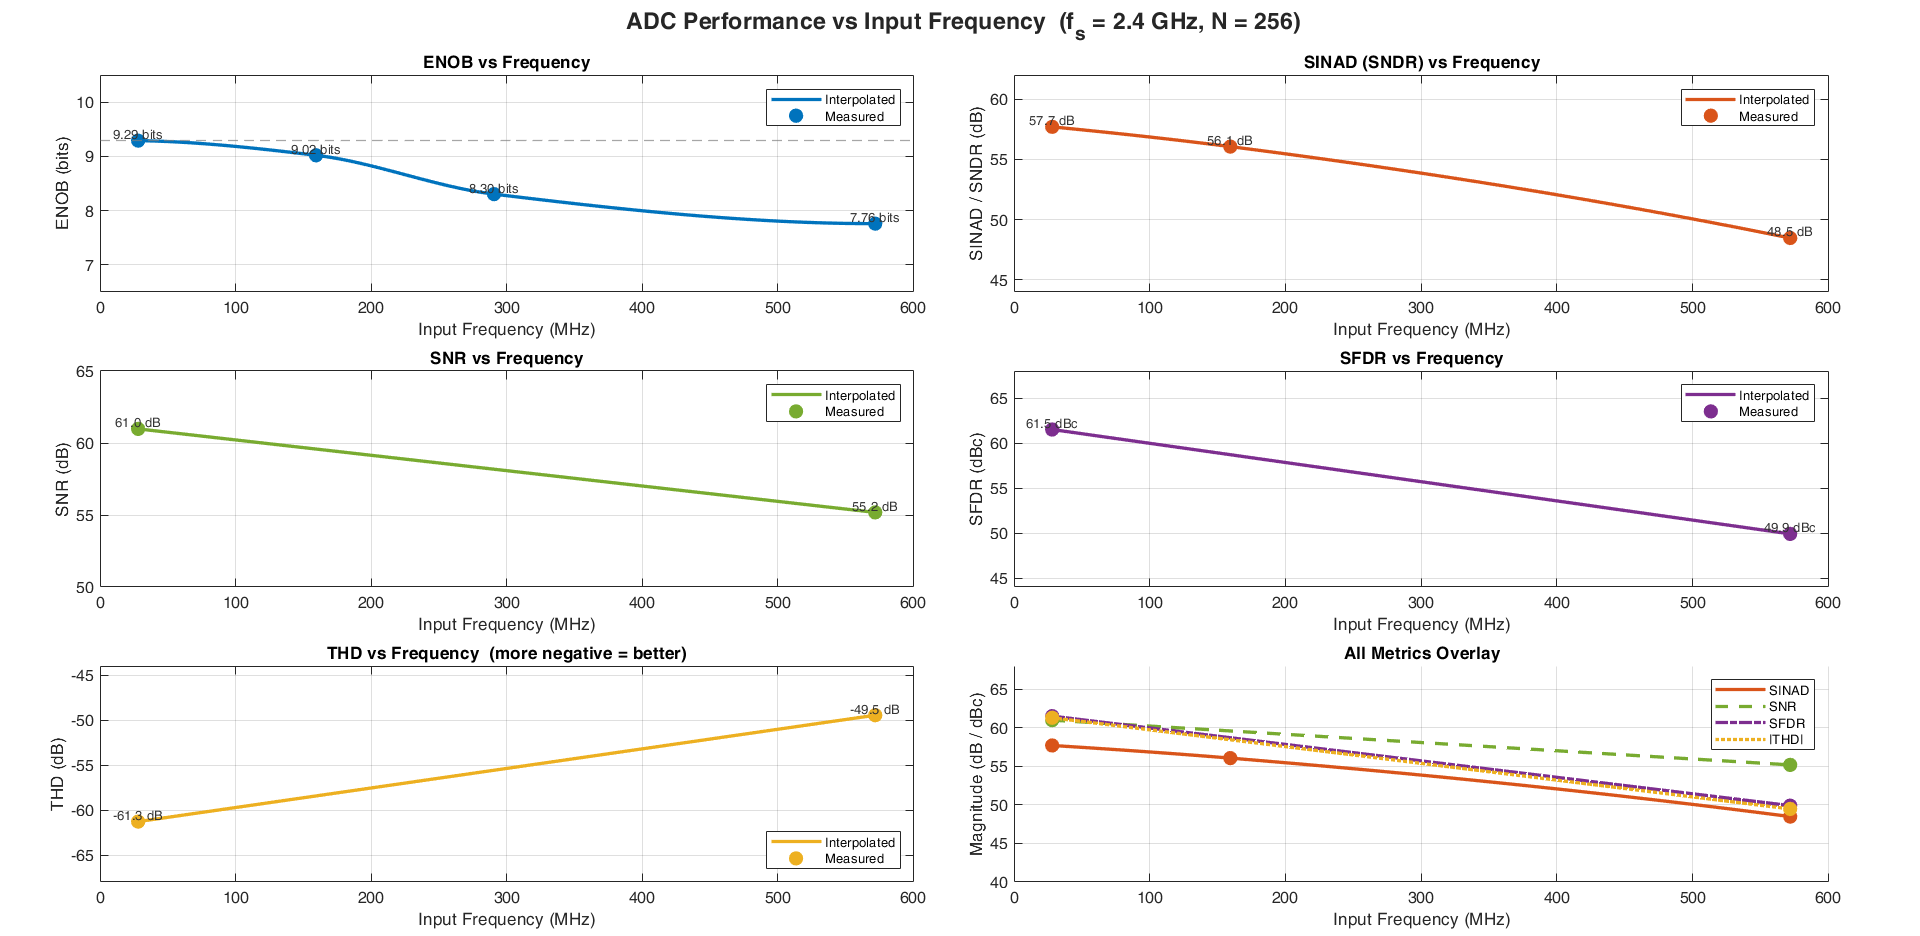
\includegraphics[width=0.8\textwidth]{chapter5/images/34.png}
	\caption{Key ADC metrics vs.\ input frequency --- FF corner}
	\label{fig:metrics_ff}
\end{figure}

\begin{figure}[h!]
	\centering
	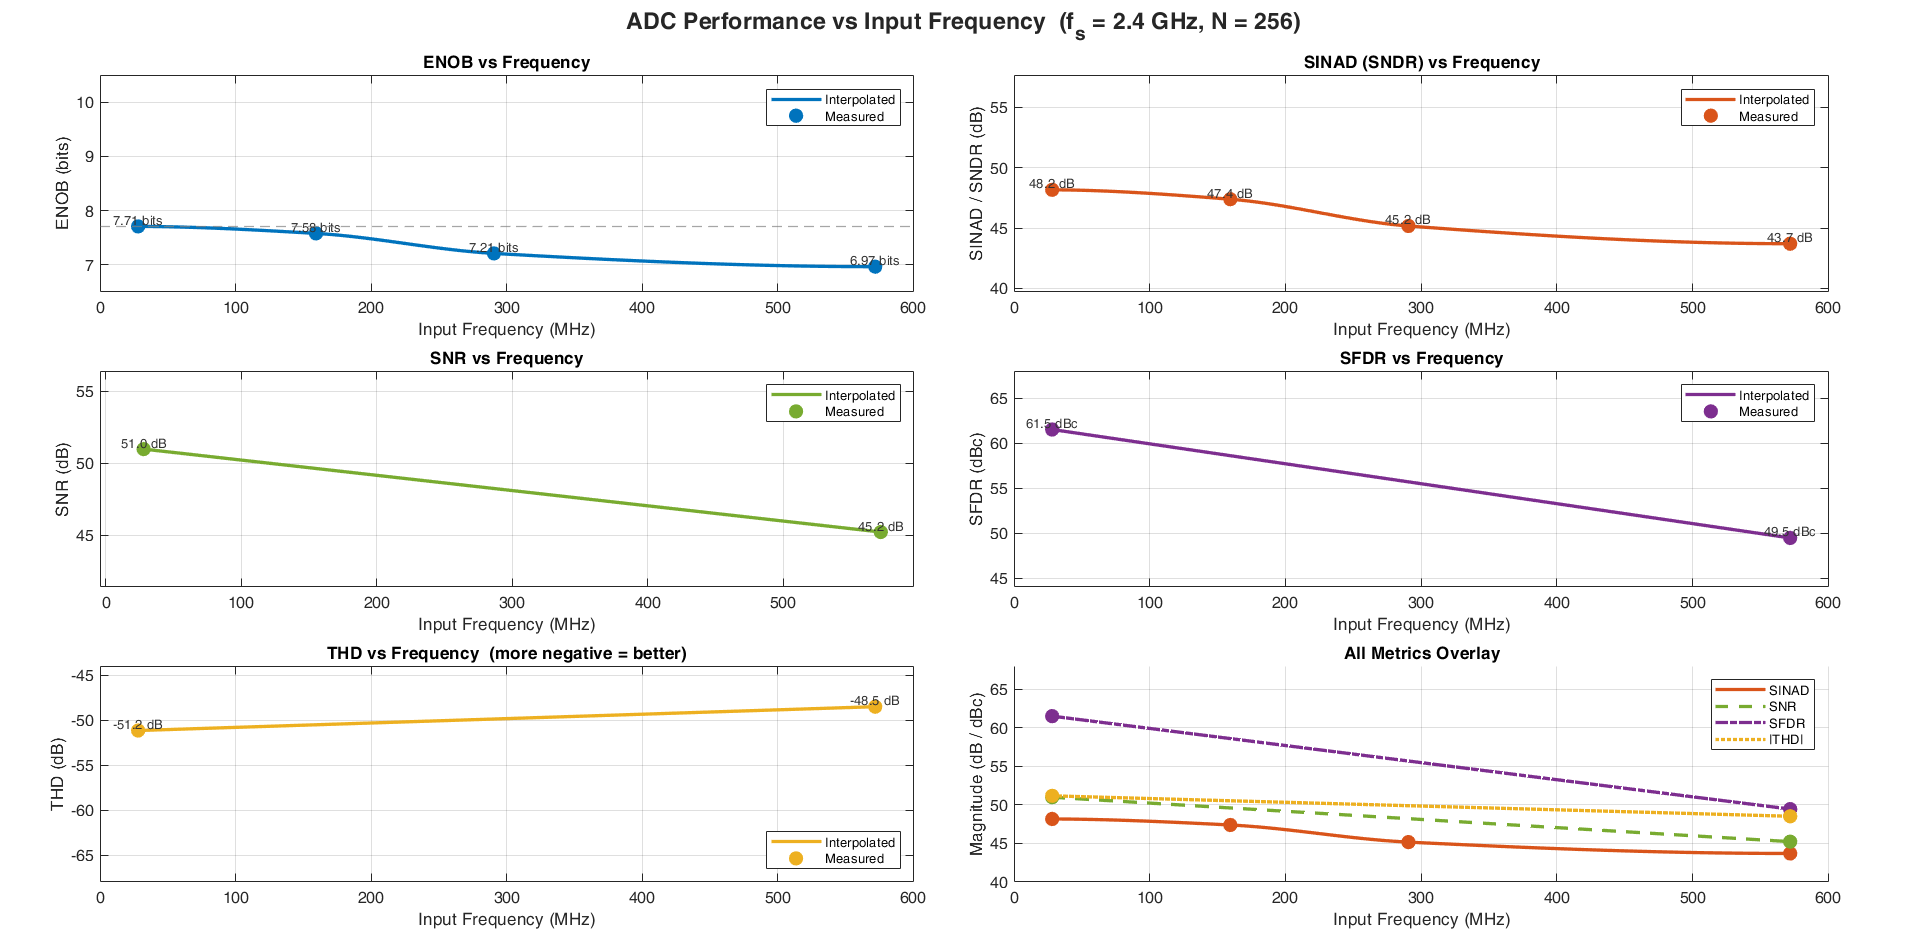
\includegraphics[width=0.8\textwidth]{chapter5/images/35.png}
	\caption{Key ADC metrics vs.\ input frequency --- SS corner}
	\label{fig:metrics_ss}
\end{figure}

Across all three corners, the metrics are favourable at low input frequencies but degrade at
higher frequencies. This is expected: the individual slice bandwidth is \SI{300}{MHz}, so
input signals approaching the \SI{600}{MHz} Nyquist limit of the TI system present a
challenging sampling scenario for the input switches. Because the aggregate sampling rate is
\SI{2.4}{GHz}, which is four times the maximum input frequency, a digital low-pass filter
applied in post-processing could suppress out-of-band noise and improve the effective SNR,
SNDR, and ENOB.



\subsection{Power Consumption}

The total power consumption of the TI ADC is estimated by computing the dynamic power of a
single slice and multiplying by 8. Dynamic power is dominated by the large-swing switching
activity within the CDAC and SAR logic, and scales linearly with frequency. The worst-case
input is $V_{\mathrm{in}} = \SI{-800}{mV}$, because the comparator output toggles from high
to low on every conversion cycle, maximising the switching energy. At this condition:

\begin{figure}[h!]
	\centering
	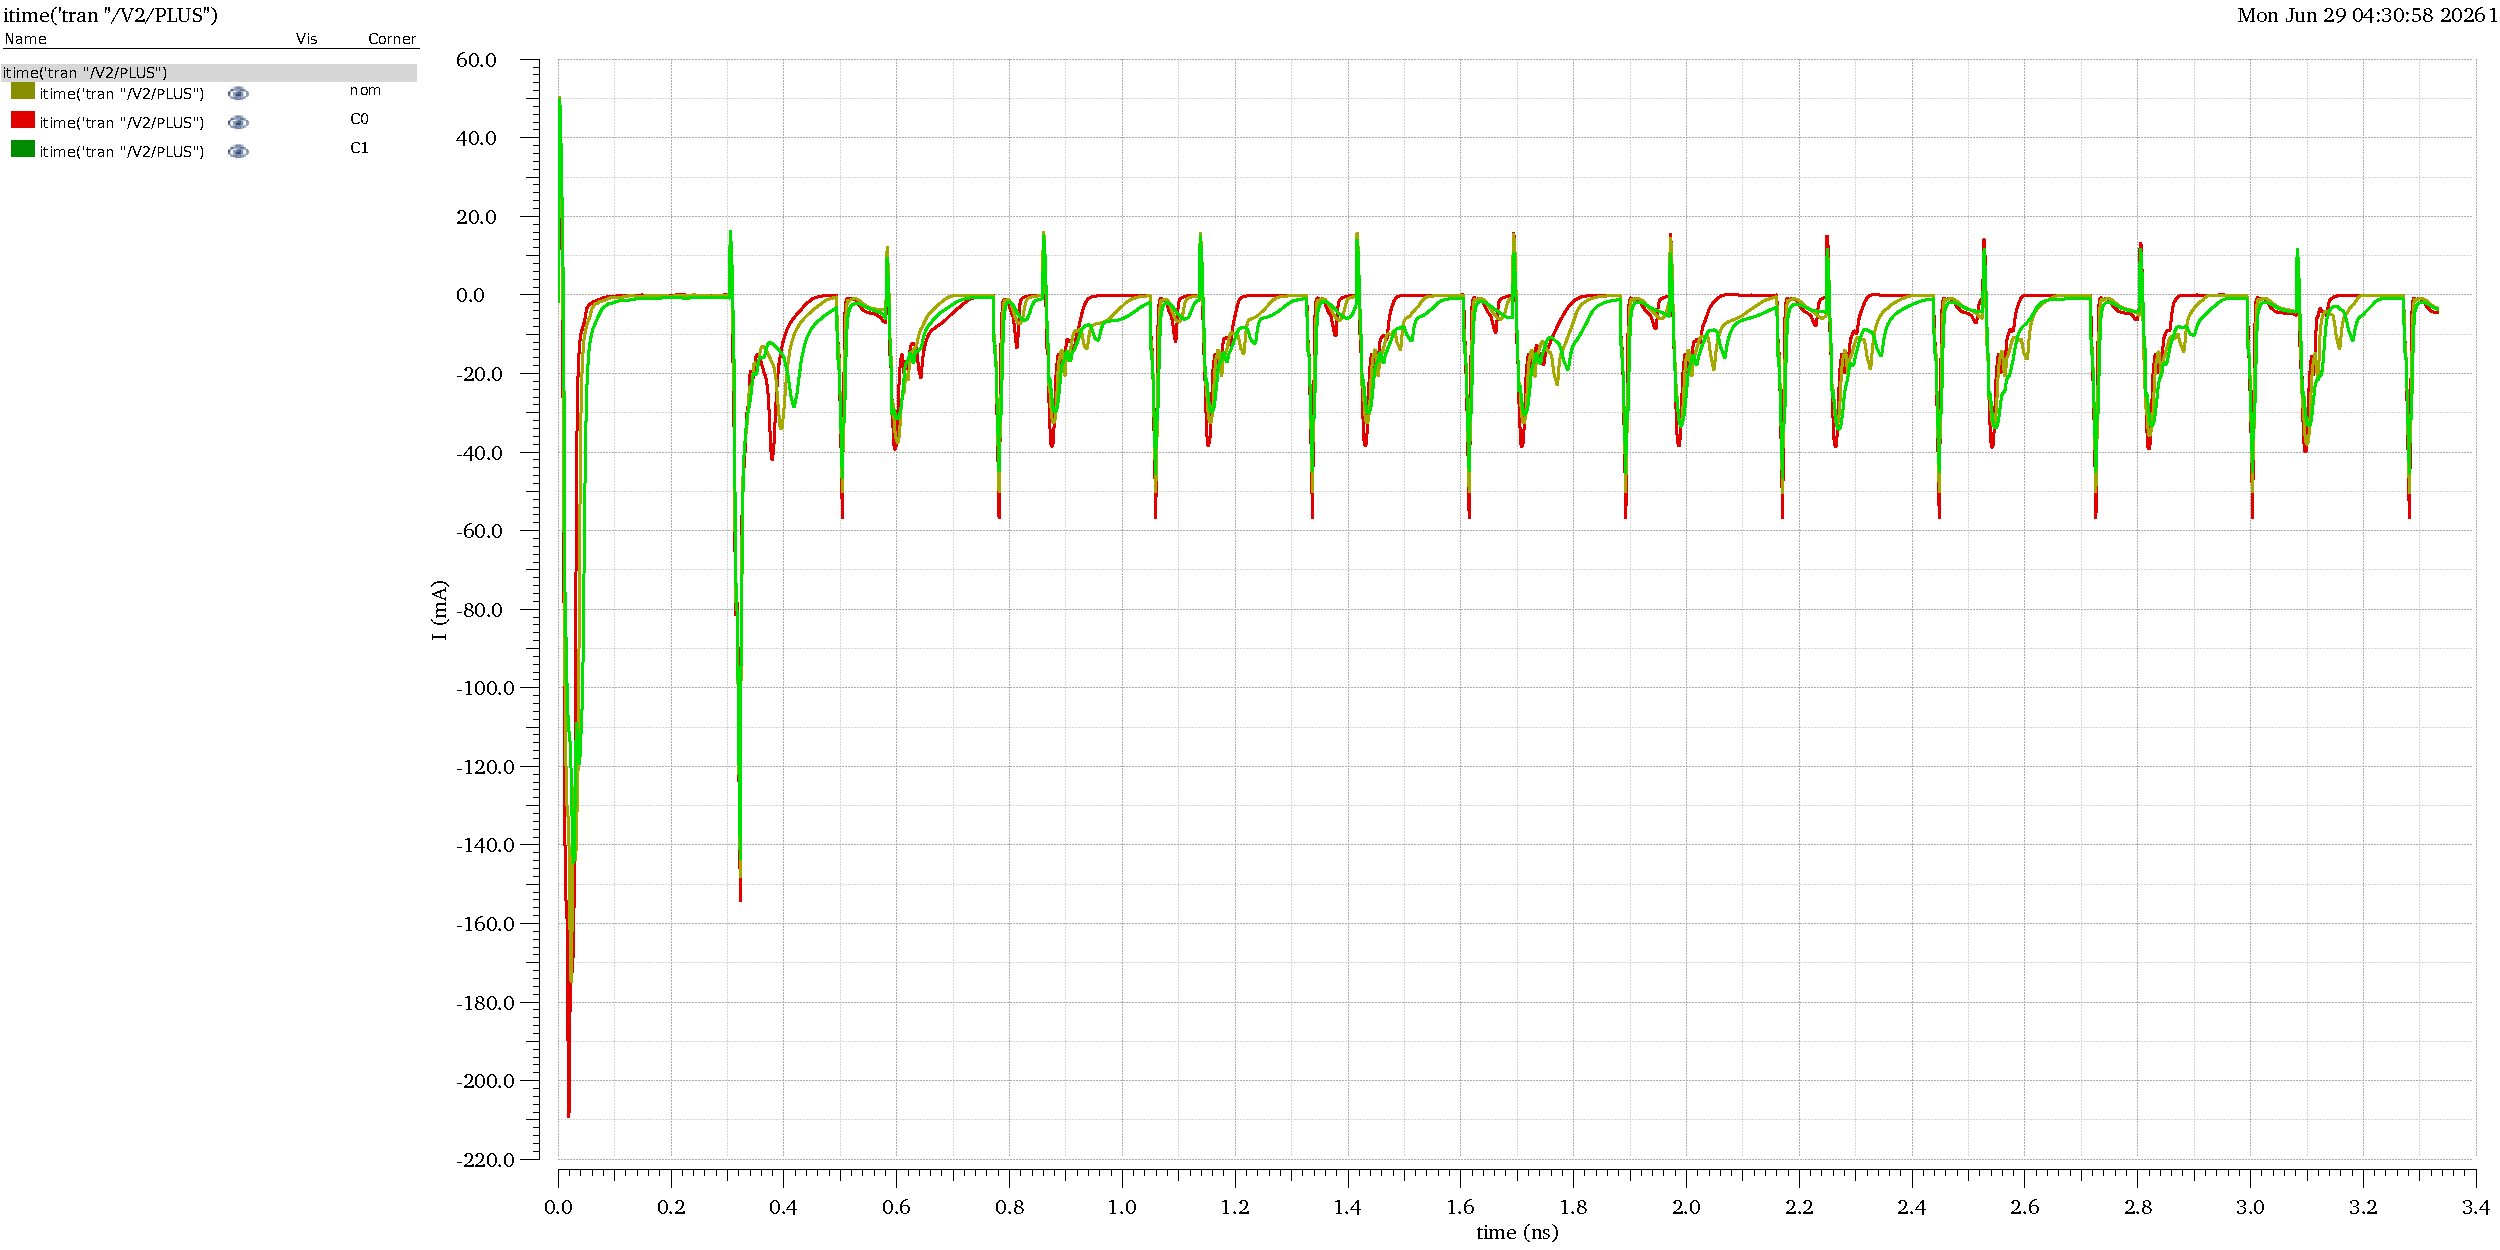
\includegraphics[width=0.75\textwidth]{chapter5/images/36.pdf}
	\caption{Dynamic supply current for one slice at $V_{\mathrm{in}} = \SI{-800}{mV}$}
	\label{fig:dynamic_current}
\end{figure}

\begin{align}
	P_{\mathrm{dyn,slice}} &= V_{DD} \times \bar{I} = V_{DD} \times \SI{9.11}{mA} = \SI{7.288}{mW} \\[4pt]
	P_{\mathrm{dyn,total}} &= 8 \times P_{\mathrm{dyn,slice}} = \SI{58.3}{mW}
\end{align}

The two standard figures of merit are then

\begin{align}
	\mathrm{FoM}_{\mathrm{Walden}}  &= \frac{P_{\mathrm{ADC}}}{2^{\mathrm{ENOB}} \times f_s}
	= \frac{\SI{58.3}{mW}}{2^{9.39} \times \SI{2.4}{GHz}}
	= \SI{36.2}{fJ/conversion\text{-}step} \\[6pt]
	\mathrm{FoM}_{\mathrm{Schreier}} &= \mathrm{SNR_{dB}} + 10\log\!\left(\frac{f_s/2}{P_{\mathrm{ADC}}}\right)
	= 60.8 + 10\log\!\left(\frac{\SI{1.2}{GHz}}{\SI{58.3}{mW}}\right)
	= \SI{163.9}{dB}
\end{align}

\begin{figure}[h!]
	\centering
	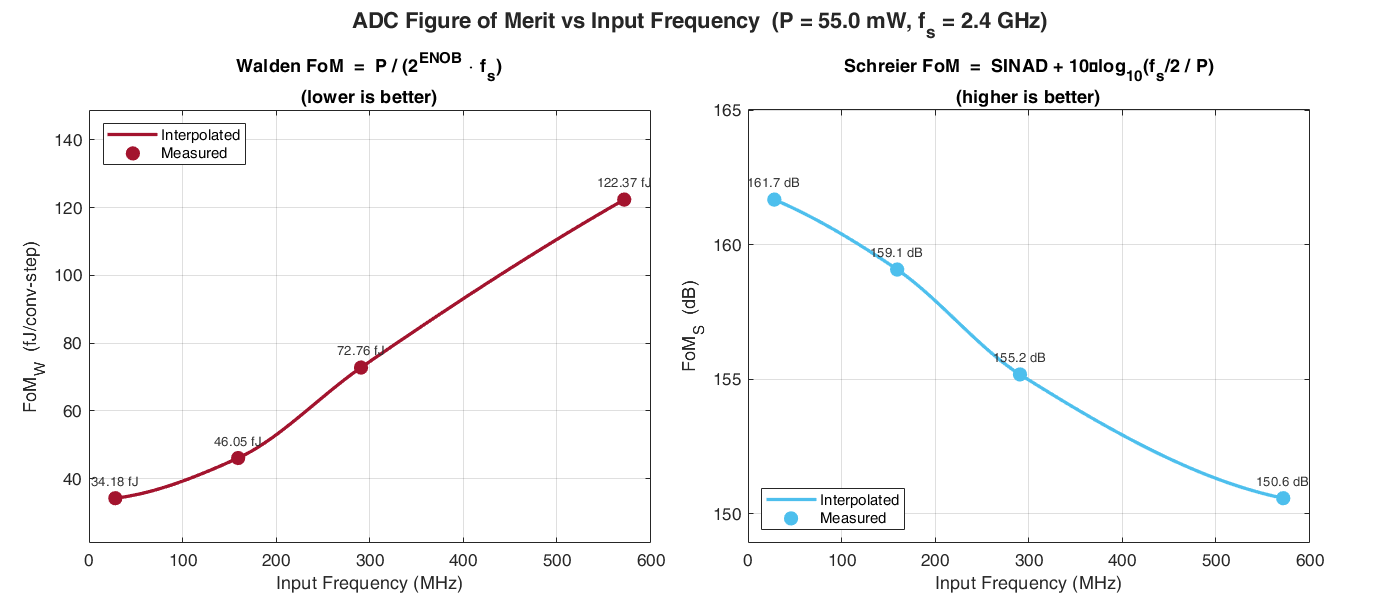
\includegraphics[width=0.8\textwidth]{chapter5/images/37.png}
	\caption{FoM vs.\ input frequency --- typical corner}
	\label{fig:fom_typ}
\end{figure}

\begin{figure}[h!]
	\centering
	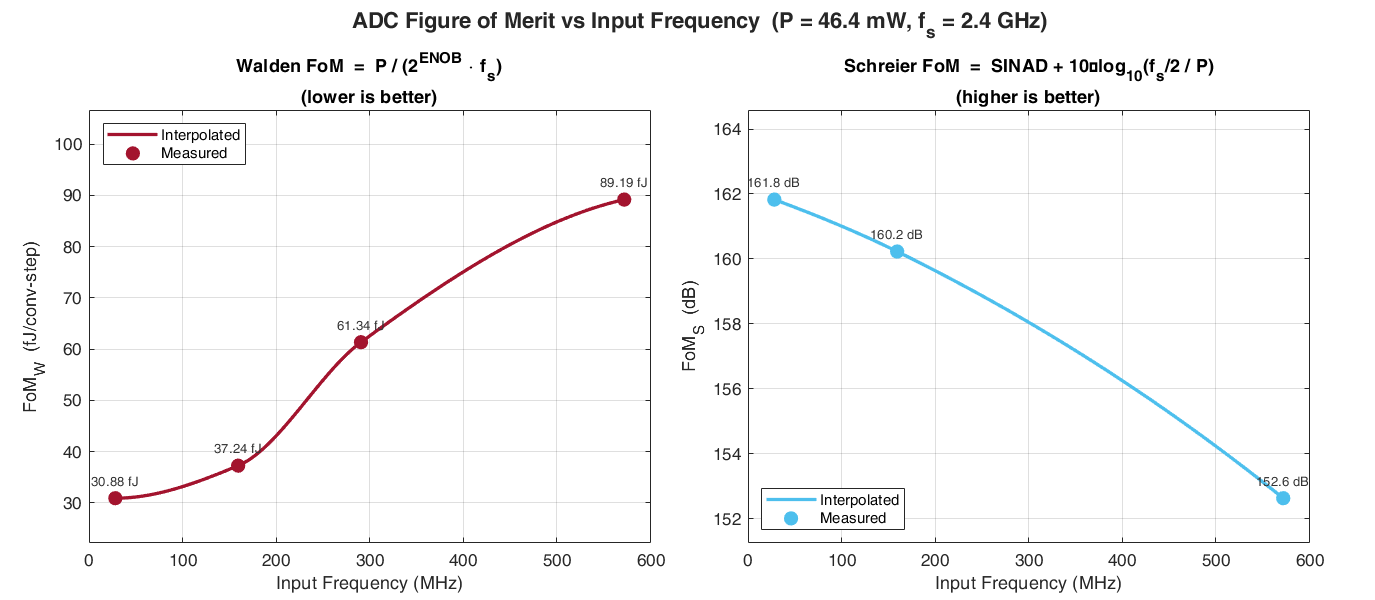
\includegraphics[width=0.8\textwidth]{chapter5/images/38.png}
	\caption{FoM vs.\ input frequency --- SS corner (\SI{125}{\celsius})}
	\label{fig:fom_ss}
\end{figure}

\begin{figure}[h!]
	\centering
	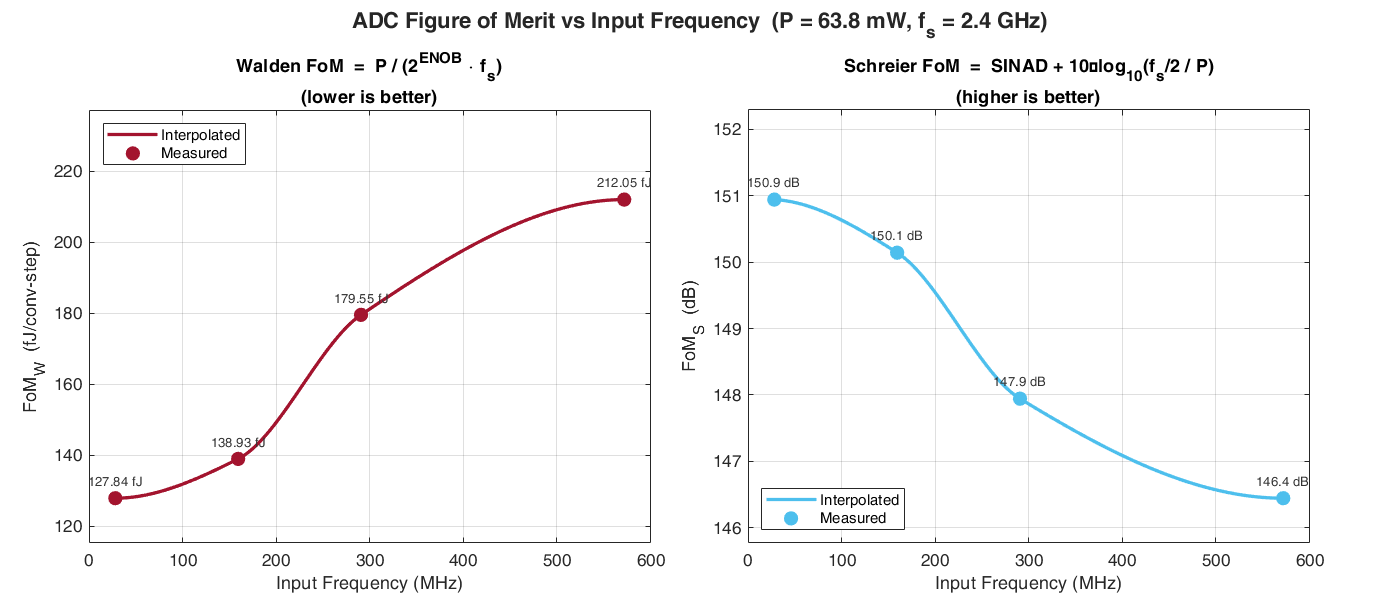
\includegraphics[width=0.8\textwidth]{chapter5/images/39.png}
	\caption{FoM vs.\ input frequency --- FF corner (\SI{-40}{\celsius})}
	\label{fig:fom_ff}
\end{figure}

\subsection{Noise Spectral Density}

As the sampling frequency increases, quantisation noise spreads over a wider bandwidth,
reducing its power spectral density. The noise spectral density (NSD) is related to the SNR by

\begin{equation}
	\mathrm{NSD} = -\mathrm{SNR_{dB}} + 10\log\!\left(\frac{f_s}{2}\right)
\end{equation}

For the best-case (typical) and worst-case (SS corner) conditions:

\begin{align}
	\mathrm{NSD_{best}} &= -60.8 + 10\log(\SI{1.2}{GHz}) = \SI{-151.6}{dBFS/Hz} \\[4pt]
	\mathrm{NSD_{worst}} &= -60.8 + 10\log(\SI{1.2}{GHz}) = \SI{-143.9}{dBFS/Hz}
\end{align}

\section{Conclusion}
% ══════════════════════════════════════════════════════════════════════════════

The SAR ADC is a highly efficient topology well suited to advanced CMOS nodes, offering an
attractive balance between speed and power consumption. A single-slice conversion rate of
\SI{300}{MHz} is a competitive result at 22\,nm, and time-interleaving scales this to an
aggregate rate of \SI{2.4}{GHz} while preserving the inherent energy efficiency of the SAR
architecture.

Table~\ref{tab:summary} summarises the achieved performance against the design targets.

\begin{table}[h!]
	\centering
	\caption{TI SAR ADC performance summary}
	\label{tab:summary}
	\renewcommand{\arraystretch}{1.3}
	\begin{tabular}{lcccc}
		\toprule
		\textbf{Parameter} & \textbf{Target} & \textbf{Best case} &
		\textbf{Worst case} ($f_{\mathrm{in}} = f_s/4$) & \textbf{Unit} \\
		\midrule
		Input full scale      & $-10$  & $-10$   & $-10$   & dBm \\
		Resolution            & 10     & 10      & 10      & bits \\
		Sampling rate         & $>2.4$ & 2.4     & 2.4     & GHz \\
		NSD                   & $-149$ & $-156.6$ & $-148.85$ & dBFS/Hz \\
		ENOB                  & ---    & 9.39    & 7.56    & bits \\
		$\mathrm{FoM_{Walden}}$  & ---  & 34.18    & 122.3   & fJ/conv-step \\
		$\mathrm{FoM_{Schreier}}$ & --- & 161.7  & 150.6   & dB \\
		Power consumption     & ---    & 46    & 56    & mW \\
		\bottomrule
	\end{tabular}
\end{table}

% ══════════════════════════════════════════════════════════════════════════════
\section{Future Work}
% ══════════════════════════════════════════════════════════════════════════════

The current implementation represents a functional proof-of-concept at the circuit-simulation
level. Several tasks remain before a tape-out-ready design can be completed:

\begin{itemize}
	\item Design and integration of a physical input buffer for each interleaved slice.
	\item Design of the multiphase clock distribution network for the sampling clocks.
	\item Full layout of the complete TI SAR ADC, including parasitics extraction.
	\item Post-layout simulations to verify performance under realistic interconnect conditions.
\end{itemize}

The results presented in this thesis provide a strong foundation and a reliable performance
estimate to guide the subsequent stages of the design.


\end{document}

